\chapter{Practical issues at the realisation of robot control}
When implementing a \ac{CT} controller, often a digital realisation of the controller is needed. For the design of a digital controller, the robot dynamics need to be discretised. This results in very complex dynamic equations for which the design of a controller is complicated. Also the discretisation of an existing controller cannot be applied to a \ac{CT} controller, as this type of controller is a nonlinear one. Therefore, the transformation is done by approximation. This means, the continuous control law of the \ac{CT} controller is used as its discrete equivalent. To show the influence of the used sampling time, some simulations are made. As controller, the \ac{CT} controller with the PD controller in the outer loop is used, as already shown in section \ref{sec:ch2_1}. The controller parameters are set to $k_{p,i} = 100$ and $k_{d,i} = 20$. For the simulations, only the sampling time of the controller is changed, so that the simulated robot still used variable step size. In this way, it can still be seen as an continuous system. If the controller would be implemented on a real robot, this system would also be a continuous one. Therefore, the results obtained in this way of simulation are more realistic.\\
For the implementation of the discrete \ac{CT} controller, different sampling times are used. The first simulation uses a sampling time of $T_s = 1\,\mathrm{ms}$, the second a sampling time of $T_s = 50\,\mathrm{ms}$ and the third uses $T_s = 100\,\mathrm{ms}$.\\
Figure \ref{fig:ch4_sim1} shows the results of the simulation with a settling time of $T_s = 1\,\mathrm{ms}$. With this sampling time, the results are very similar to the original result, with the continuous control law, as it can be seen in Figure \ref{fig:ch2_sim1}.
\begin{figure}[H]
	\centering
	% This file was created by matlab2tikz v0.4.3.
% Copyright (c) 2008--2013, Nico Schlömer <nico.schloemer@gmail.com>
% All rights reserved.
% 
% The latest updates can be retrieved from
%   http://www.mathworks.com/matlabcentral/fileexchange/22022-matlab2tikz
% where you can also make suggestions and rate matlab2tikz.
% 
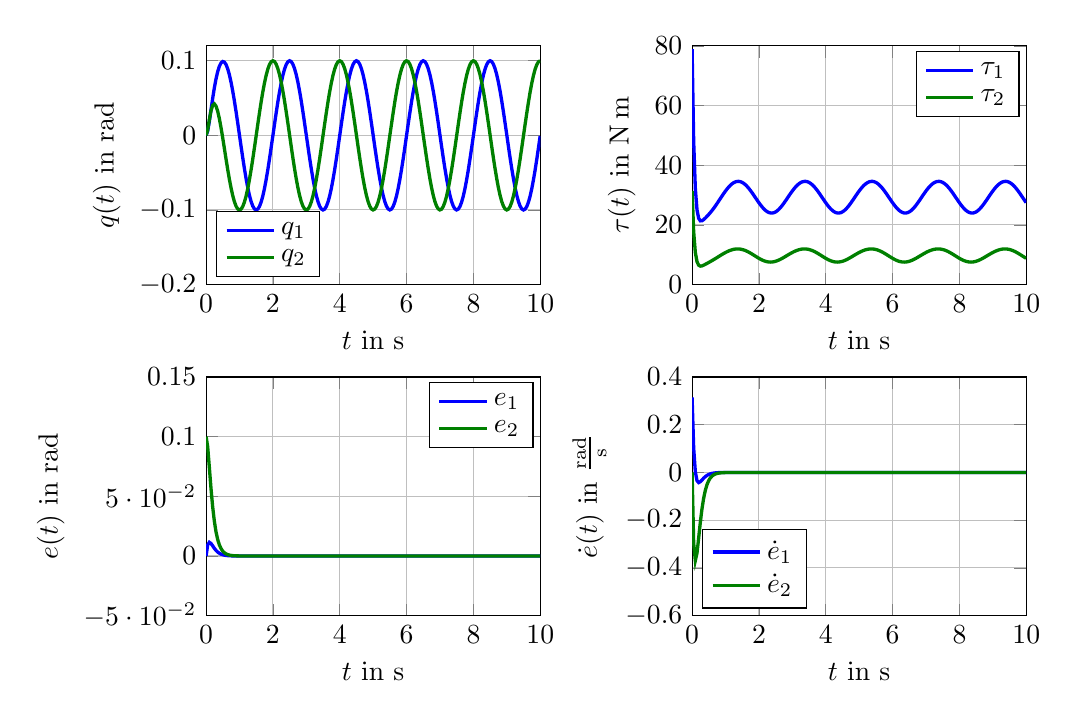
\begin{tikzpicture}

\begin{axis}[%
width=0.35\textwidth,
height=0.25\textwidth,
scale only axis,
xmin=0,
xmax=10,
xlabel={$t$ in $\mathrm{s}$},
xmajorgrids,
ymin=-0.2,
ymax=0.12,
ylabel={$q(t)$ in $\mathrm{rad}$},
ymajorgrids,
name=plot1,
legend style={at={(0.03,0.03)},anchor=south west,draw=black,fill=white,legend cell align=left}
]
\addplot [
color=blue,
solid,
line width=1.2pt
]
table[row sep=crcr]{
0 0\\
0.047 0.00551556594291563\\
0.097 0.0185311613117965\\
0.147 0.0340437241341994\\
0.197 0.0494907672076347\\
0.247 0.0635754868138459\\
0.297 0.0756389609341111\\
0.347 0.0853412589097447\\
0.397 0.0925055194801475\\
0.447 0.0970459967440627\\
0.497 0.0989378684813178\\
0.547 0.0982066365104553\\
0.597 0.09492573090746\\
0.647 0.0892166546490732\\
0.697 0.0812489969799424\\
0.747 0.0712391773632141\\
0.797 0.059447549073368\\
0.847 0.0461738632952497\\
0.897 0.0317512670401012\\
0.947 0.0165390829293212\\
0.997 0.000914647301158047\\
1.047 -0.0147355098130312\\
1.097 -0.0300248620007804\\
1.147 -0.0445761879139116\\
1.197 -0.0580307147122446\\
1.247 -0.0700568554310594\\
1.297 -0.0803583094752841\\
1.347 -0.088681316163788\\
1.397 -0.0948208755067011\\
1.447 -0.0986257781018044\\
1.497 -0.10000231688734\\
1.547 -0.0989165870077874\\
1.597 -0.0953953155957917\\
1.647 -0.0895252000775557\\
1.697 -0.0814507708082953\\
1.747 -0.0713708305274944\\
1.797 -0.0595335583771079\\
1.847 -0.0462303991775472\\
1.897 -0.0317888885102823\\
1.947 -0.0165645902137704\\
1.997 -0.000932344569772873\\
2.047 0.0147229577422568\\
2.097 0.0300158492863281\\
2.147 0.0445697744126209\\
2.197 0.0580263595913222\\
2.247 0.0700542376661312\\
2.297 0.080357208934547\\
2.347 0.0886815380357744\\
2.397 0.0948222066296641\\
2.447 0.0986279673042042\\
2.497 0.100005073476422\\
2.547 0.0989195925794429\\
2.597 0.0953982447920131\\
2.647 0.089527746111297\\
2.697 0.0814526717610876\\
2.747 0.0713718927773497\\
2.797 0.0595336741208476\\
2.847 0.0462295558719421\\
2.897 0.0317871690949177\\
2.947 0.0165621640739855\\
2.997 0.000929450218277787\\
3.047 -0.0147260364522077\\
3.097 -0.0300188110245551\\
3.147 -0.0445723296205671\\
3.197 -0.0580282583867531\\
3.247 -0.0700552938639655\\
3.297 -0.0803573180153623\\
3.347 -0.0886806874120365\\
3.397 -0.0948204771998271\\
3.447 -0.0986255260253792\\
3.497 -0.100002157497432\\
3.547 -0.0989164863054691\\
3.597 -0.0953952520185032\\
3.647 -0.0895251599650011\\
3.697 -0.0814507455150588\\
3.747 -0.0713708145869846\\
3.797 -0.0595335483355872\\
3.847 -0.0462303928545997\\
3.897 -0.0317888845302806\\
3.947 -0.0165645877093423\\
3.997 -0.000932342994300433\\
4.047 0.0147229587330948\\
4.097 0.0300158499093371\\
4.147 0.0445697748042665\\
4.197 0.0580263598374756\\
4.247 0.0700542378208119\\
4.297 0.0803572090317292\\
4.347 0.0886815380968211\\
4.397 0.094822206668005\\
4.447 0.0986279673282806\\
4.497 0.100005073491538\\
4.547 0.0989195925889324\\
4.597 0.0953982447979693\\
4.647 0.089527746115035\\
4.697 0.0814526717634332\\
4.747 0.0713718927788213\\
4.797 0.059533674121771\\
4.847 0.0462295558725211\\
4.897 0.0317871690952809\\
4.947 0.0165621640742134\\
4.997 0.000929450218420655\\
5.047 -0.014726036452118\\
5.097 -0.030018811024499\\
5.147 -0.0445723296205319\\
5.197 -0.058028258386731\\
5.247 -0.0700552938639517\\
5.297 -0.0803573180153536\\
5.347 -0.0886806874120312\\
5.397 -0.0948204771998238\\
5.447 -0.0986255260253771\\
5.497 -0.100002157497431\\
5.547 -0.0989164863054684\\
5.597 -0.0953952520185026\\
5.647 -0.0895251599650008\\
5.697 -0.0814507455150586\\
5.747 -0.0713708145869844\\
5.797 -0.0595335483355872\\
5.847 -0.0462303928545995\\
5.897 -0.0317888845302805\\
5.947 -0.0165645877093423\\
5.997 -0.000932342994300425\\
6.047 0.0147229587330948\\
6.097 0.0300158499093371\\
6.147 0.0445697748042665\\
6.197 0.0580263598374756\\
6.247 0.0700542378208118\\
6.297 0.0803572090317292\\
6.347 0.0886815380968211\\
6.397 0.094822206668005\\
6.447 0.0986279673282806\\
6.497 0.100005073491538\\
6.547 0.0989195925889324\\
6.597 0.0953982447979693\\
6.647 0.089527746115035\\
6.697 0.0814526717634332\\
6.747 0.0713718927788213\\
6.797 0.059533674121771\\
6.847 0.0462295558725211\\
6.897 0.0317871690952809\\
6.947 0.0165621640742134\\
6.997 0.000929450218420668\\
7.047 -0.0147260364521179\\
7.097 -0.030018811024499\\
7.147 -0.0445723296205319\\
7.197 -0.058028258386731\\
7.247 -0.0700552938639517\\
7.297 -0.0803573180153536\\
7.347 -0.0886806874120312\\
7.397 -0.0948204771998238\\
7.447 -0.0986255260253771\\
7.497 -0.100002157497431\\
7.547 -0.0989164863054683\\
7.597 -0.0953952520185027\\
7.647 -0.0895251599650009\\
7.697 -0.0814507455150586\\
7.747 -0.0713708145869845\\
7.797 -0.059533548335587\\
7.847 -0.0462303928545996\\
7.897 -0.0317888845302806\\
7.947 -0.0165645877093423\\
7.997 -0.000932342994300464\\
8.047 0.014722958733095\\
8.097 0.0300158499093368\\
8.147 0.0445697748042664\\
8.197 0.0580263598374757\\
8.247 0.0700542378208117\\
8.297 0.0803572090317294\\
8.347 0.088681538096821\\
8.397 0.094822206668005\\
8.447 0.0986279673282807\\
8.497 0.100005073491538\\
8.547 0.0989195925889324\\
8.597 0.0953982447979694\\
8.647 0.089527746115035\\
8.697 0.0814526717634331\\
8.747 0.0713718927788214\\
8.797 0.0595336741217708\\
8.847 0.0462295558725214\\
8.897 0.031787169095281\\
8.947 0.0165621640742131\\
8.997 0.000929450218420708\\
9.047 -0.0147260364521182\\
9.097 -0.0300188110244987\\
9.147 -0.0445723296205319\\
9.197 -0.0580282583867312\\
9.247 -0.0700552938639517\\
9.297 -0.0803573180153538\\
9.347 -0.0886806874120311\\
9.397 -0.0948204771998238\\
9.447 -0.0986255260253772\\
9.497 -0.100002157497431\\
9.547 -0.0989164863054683\\
9.597 -0.0953952520185028\\
9.647 -0.0895251599650009\\
9.697 -0.0814507455150585\\
9.747 -0.0713708145869844\\
9.797 -0.0595335483355869\\
9.847 -0.0462303928545998\\
9.897 -0.0317888845302806\\
9.947 -0.016564587709342\\
9.997 -0.00093234299430046\\
};
\addlegendentry{$q_1$};

\addplot [
color=green!50!black,
solid,
line width=1.2pt
]
table[row sep=crcr]{
0 0\\
0.047 0.00710020907413783\\
0.097 0.0208627761080444\\
0.147 0.0329197725365565\\
0.197 0.040213407128243\\
0.247 0.0421718843154133\\
0.297 0.0392807459984606\\
0.347 0.0323999875248439\\
0.397 0.0224581378423865\\
0.447 0.0103300012252933\\
0.497 -0.00320109537882808\\
0.547 -0.017445885667916\\
0.597 -0.0318000050636197\\
0.647 -0.0457333661326845\\
0.697 -0.0587819045527103\\
0.747 -0.0705425502277979\\
0.797 -0.0806710295869404\\
0.847 -0.0888816893846275\\
0.897 -0.0949484911034588\\
0.947 -0.0987064327856958\\
0.997 -0.100052806412141\\
1.047 -0.098947848659032\\
1.097 -0.0954144747731861\\
1.147 -0.0895368961326849\\
1.197 -0.0814580136031901\\
1.247 -0.0713755542701589\\
1.297 -0.0595369816009595\\
1.347 -0.0462332609791953\\
1.397 -0.0317916055317624\\
1.447 -0.0165673622896967\\
1.497 -0.000935226585236228\\
1.547 0.0147200064954162\\
1.597 0.0300129306323746\\
1.647 0.0445670262511978\\
1.697 0.0580239363066376\\
1.747 0.0700522931936279\\
1.797 0.0803558808372466\\
1.847 0.0886809320687442\\
1.897 0.0948223823037956\\
1.947 0.0986289257845143\\
1.997 0.100006749654503\\
2.047 0.0989218532594969\\
2.097 0.0954008945758873\\
2.147 0.0895305417586559\\
2.197 0.0814553446027978\\
2.247 0.0713741773289501\\
2.297 0.0595353396283467\\
2.347 0.0462304364400694\\
2.397 0.0317871876148205\\
2.447 0.0165613456092527\\
2.497 0.000927921873374083\\
2.547 -0.0147280600475204\\
2.597 -0.0300210550185941\\
2.647 -0.0445744951367223\\
2.697 -0.0580300620967637\\
2.747 -0.0700565048341233\\
2.797 -0.080357786290143\\
2.847 -0.0886803603695215\\
2.897 -0.0948194019190425\\
2.947 -0.0986238382733948\\
2.997 -0.10000006001095\\
3.047 -0.0989142204530324\\
3.097 -0.0953930674953057\\
3.147 -0.0895232868817891\\
3.197 -0.0814493722450757\\
3.247 -0.0713700732972566\\
3.297 -0.0595335085774624\\
3.347 -0.046231062243246\\
3.397 -0.0317902146524432\\
3.447 -0.0165664830892889\\
3.497 -0.000934671198944757\\
3.547 0.0147203571134349\\
3.597 0.0300131518525216\\
3.647 0.0445671657540668\\
3.697 0.0580240242339558\\
3.747 0.0700523485871523\\
3.797 0.0803559157190907\\
3.847 0.088680954024829\\
3.897 0.0948223961182748\\
3.947 0.0986289344730607\\
3.997 0.100006755117129\\
4.047 0.0989218566927558\\
4.097 0.0954008967329927\\
4.147 0.08953054311355\\
4.197 0.0814553454535789\\
4.247 0.071374177863045\\
4.297 0.0595353399635565\\
4.347 0.046230436650409\\
4.397 0.0317871877467802\\
4.447 0.0165613456920249\\
4.497 0.000927921925285063\\
4.547 -0.0147280600149687\\
4.597 -0.030021054998185\\
4.647 -0.0445744951239275\\
4.697 -0.0580300620887433\\
4.747 -0.0700565048290963\\
4.797 -0.0803577862869924\\
4.847 -0.0886803603675471\\
4.897 -0.0948194019178054\\
4.947 -0.0986238382726196\\
4.997 -0.100000060010465\\
5.047 -0.0989142204527281\\
5.097 -0.095393067495115\\
5.147 -0.0895232868816697\\
5.197 -0.0814493722450009\\
5.247 -0.0713700732972097\\
5.297 -0.0595335085774331\\
5.347 -0.0462310622432275\\
5.397 -0.0317902146524317\\
5.447 -0.0165664830892817\\
5.497 -0.000934671198940289\\
5.547 0.0147203571134376\\
5.597 0.0300131518525235\\
5.647 0.0445671657540679\\
5.697 0.0580240242339565\\
5.747 0.0700523485871527\\
5.797 0.0803559157190908\\
5.847 0.0886809540248292\\
5.897 0.0948223961182748\\
5.947 0.0986289344730607\\
5.997 0.100006755117129\\
6.047 0.0989218566927558\\
6.097 0.0954008967329927\\
6.147 0.08953054311355\\
6.197 0.0814553454535789\\
6.247 0.071374177863045\\
6.297 0.0595353399635565\\
6.347 0.046230436650409\\
6.397 0.0317871877467802\\
6.447 0.016561345692025\\
6.497 0.000927921925285095\\
6.547 -0.0147280600149687\\
6.597 -0.0300210549981849\\
6.647 -0.0445744951239275\\
6.697 -0.0580300620887433\\
6.747 -0.0700565048290963\\
6.797 -0.0803577862869924\\
6.847 -0.0886803603675471\\
6.897 -0.0948194019178053\\
6.947 -0.0986238382726196\\
6.997 -0.100000060010465\\
7.047 -0.0989142204527281\\
7.097 -0.095393067495115\\
7.147 -0.0895232868816697\\
7.197 -0.0814493722450009\\
7.247 -0.0713700732972097\\
7.297 -0.0595335085774331\\
7.347 -0.0462310622432275\\
7.397 -0.0317902146524317\\
7.447 -0.0165664830892817\\
7.497 -0.000934671198940303\\
7.547 0.0147203571134378\\
7.597 0.0300131518525235\\
7.647 0.0445671657540679\\
7.697 0.0580240242339565\\
7.747 0.0700523485871527\\
7.797 0.080355915719091\\
7.847 0.0886809540248292\\
7.897 0.0948223961182749\\
7.947 0.0986289344730607\\
7.997 0.100006755117129\\
8.047 0.0989218566927558\\
8.097 0.0954008967329928\\
8.147 0.08953054311355\\
8.197 0.0814553454535788\\
8.247 0.0713741778630451\\
8.297 0.0595353399635564\\
8.347 0.0462304366504093\\
8.397 0.0317871877467803\\
8.447 0.0165613456920247\\
8.497 0.000927921925285118\\
8.547 -0.014728060014969\\
8.597 -0.0300210549981846\\
8.647 -0.0445744951239274\\
8.697 -0.0580300620887434\\
8.747 -0.0700565048290963\\
8.797 -0.0803577862869925\\
8.847 -0.0886803603675469\\
8.897 -0.0948194019178052\\
8.947 -0.0986238382726195\\
8.997 -0.100000060010465\\
9.047 -0.098914220452728\\
9.097 -0.0953930674951151\\
9.147 -0.0895232868816697\\
9.197 -0.0814493722450008\\
9.247 -0.0713700732972098\\
9.297 -0.059533508577433\\
9.347 -0.0462310622432278\\
9.397 -0.0317902146524317\\
9.447 -0.0165664830892815\\
9.497 -0.00093467119894033\\
9.547 0.0147203571134378\\
9.597 0.0300131518525232\\
9.647 0.0445671657540678\\
9.697 0.0580240242339567\\
9.747 0.0700523485871526\\
9.797 0.080355915719091\\
9.847 0.088680954024829\\
9.897 0.0948223961182749\\
9.947 0.0986289344730607\\
9.997 0.100006755117129\\
};
\addlegendentry{$q_2$};

\end{axis}

\begin{axis}[%
width=0.35\textwidth,
height=0.25\textwidth,
scale only axis,
xmin=0,
xmax=10,
xlabel={$t$ in $\mathrm{s}$},
xmajorgrids,
ymin=-0.05,
ymax=0.15,
ylabel={$e(t)$ in $\mathrm{rad}$},
ymajorgrids,
name=plot3,
at=(plot1.below south west),
anchor=above north west,
legend style={draw=black,fill=white,legend cell align=left}
]
\addplot [
color=blue,
solid,
line width=1.2pt
]
table[row sep=crcr]{
0 0\\
0.047 0.00919632524094811\\
0.097 0.0114728293123311\\
0.147 0.0105135681034902\\
0.197 0.00852267823155019\\
0.247 0.00646562826453471\\
0.297 0.00470517907710166\\
0.347 0.00332756666031095\\
0.397 0.00230467088825573\\
0.447 0.00157101687883618\\
0.497 0.00105769022957719\\
0.547 0.000705244766740859\\
0.597 0.000466934149279355\\
0.647 0.000307910183407936\\
0.697 0.000203075727108565\\
0.747 0.000134782864428057\\
0.797 9.08348974674872e-05\\
0.847 6.29118088494307e-05\\
0.897 4.53963431398668e-05\\
0.947 3.45293534907178e-05\\
0.997 2.78165421563522e-05\\
1.047 2.3618629167544e-05\\
1.097 2.08713766528153e-05\\
1.147 1.88956762219999e-05\\
1.197 1.72692730596793e-05\\
1.247 1.57403526787891e-05\\
1.297 1.41694640713452e-05\\
1.347 1.24905937323588e-05\\
1.397 1.06851382978973e-05\\
1.447 8.76447890546528e-06\\
1.497 6.75817644492371e-06\\
1.547 4.70573059116464e-06\\
1.597 2.65053905235124e-06\\
1.647 6.35245074487312e-07\\
1.697 -1.30189875557907e-06\\
1.747 -3.12970014768044e-06\\
1.797 -4.82559372765035e-06\\
1.847 -6.3759265520047e-06\\
1.897 -7.77487295888779e-06\\
1.947 -9.02206904154768e-06\\
1.997 -1.01192735414935e-05\\
2.047 -1.10665583930719e-05\\
2.097 -1.18586622005687e-05\\
2.147 -1.24821749311957e-05\\
2.197 -1.29141521372847e-05\\
2.247 -1.31225877506025e-05\\
2.297 -1.30689233342335e-05\\
2.347 -1.27124657187394e-05\\
2.397 -1.20162612608499e-05\\
2.447 -1.09536813053535e-05\\
2.497 -9.51476552686625e-06\\
2.547 -7.71130224674899e-06\\
2.597 -5.57973527377797e-06\\
2.647 -3.18127881589192e-06\\
2.697 -5.99054036709568e-07\\
2.747 2.06745029247835e-06\\
2.797 4.70984998783563e-06\\
2.847 7.21923215718512e-06\\
2.897 9.49428832337784e-06\\
2.947 1.14482088264881e-05\\
2.997 1.30136250367697e-05\\
3.047 1.41452683440173e-05\\
3.097 1.48204004274122e-05\\
3.147 1.50373828774197e-05\\
3.197 1.48129475681727e-05\\
3.247 1.41787855849201e-05\\
3.297 1.31780041495583e-05\\
3.347 1.18618419809174e-05\\
3.397 1.02868314239418e-05\\
3.447 8.51240248035678e-06\\
3.497 6.59878653722079e-06\\
3.547 4.60502827295817e-06\\
3.597 2.58696176384798e-06\\
3.647 5.95132520014863e-07\\
3.697 -1.32719199209819e-06\\
3.747 -3.14564065759249e-06\\
3.797 -4.83563524832087e-06\\
3.847 -6.38224949955218e-06\\
3.897 -7.77885296050773e-06\\
3.947 -9.0245734697264e-06\\
3.997 -1.01208490141354e-05\\
4.047 -1.10675492310999e-05\\
4.097 -1.18592852094909e-05\\
4.147 -1.24825665767589e-05\\
4.197 -1.29143982906532e-05\\
4.247 -1.31227424312735e-05\\
4.297 -1.3069020516579e-05\\
4.347 -1.27125267653933e-05\\
4.397 -1.20162996018053e-05\\
4.447 -1.09537053817471e-05\\
4.497 -9.51478064332989e-06\\
4.547 -7.71131173622763e-06\\
4.597 -5.57974122994409e-06\\
4.647 -3.18128255383243e-06\\
4.697 -5.99056382236118e-07\\
4.747 2.0674488208916e-06\\
4.797 4.70984906467131e-06\\
4.847 7.21923157804422e-06\\
4.897 9.49428796017532e-06\\
4.947 1.1448208598705e-05\\
4.997 1.3013624893926e-05\\
5.047 1.41452682543061e-05\\
5.097 1.4820400371391e-05\\
5.147 1.50373828422257e-05\\
5.197 1.48129475462597e-05\\
5.247 1.41787855711117e-05\\
5.297 1.31780041408291e-05\\
5.347 1.1861841975519e-05\\
5.397 1.02868314205418e-05\\
5.447 8.51240247826124e-06\\
5.497 6.59878653586077e-06\\
5.547 4.60502827213938e-06\\
5.597 2.58696176334838e-06\\
5.647 5.95132519612407e-07\\
5.697 -1.32719199233411e-06\\
5.747 -3.14564065791167e-06\\
5.797 -4.83563524844577e-06\\
5.847 -6.38224949974647e-06\\
5.897 -7.77885296056324e-06\\
5.947 -9.02457346960497e-06\\
5.997 -1.0120849014168e-05\\
6.047 -1.10675492311241e-05\\
6.097 -1.18592852095117e-05\\
6.147 -1.24825665767797e-05\\
6.197 -1.29143982908059e-05\\
6.247 -1.31227424312874e-05\\
6.297 -1.30690205164957e-05\\
6.347 -1.27125267653933e-05\\
6.397 -1.20162996017498e-05\\
6.447 -1.09537053817471e-05\\
6.497 -9.51478064334377e-06\\
6.547 -7.71131173621376e-06\\
6.597 -5.5797412299996e-06\\
6.647 -3.18128255376304e-06\\
6.697 -5.99056382249996e-07\\
6.747 2.06744882100263e-06\\
6.797 4.70984906467825e-06\\
6.847 7.21923157822463e-06\\
6.897 9.49428796019614e-06\\
6.947 1.14482085985454e-05\\
6.997 1.30136248939378e-05\\
7.047 1.41452682543147e-05\\
7.097 1.4820400371398e-05\\
7.147 1.50373828422326e-05\\
7.197 1.48129475462805e-05\\
7.247 1.41787855711256e-05\\
7.297 1.3178004140843e-05\\
7.347 1.1861841975519e-05\\
7.397 1.02868314205279e-05\\
7.447 8.51240247824736e-06\\
7.497 6.59878653587465e-06\\
7.547 4.60502827218101e-06\\
7.597 2.58696176336226e-06\\
7.647 5.95132519626285e-07\\
7.697 -1.32719199232023e-06\\
7.747 -3.1456406578978e-06\\
7.797 -4.83563524834862e-06\\
7.847 -6.38224949971178e-06\\
7.897 -7.77885296053549e-06\\
7.947 -9.0245734695911e-06\\
7.997 -1.01208490141534e-05\\
8.047 -1.10675492310357e-05\\
8.097 -1.18592852095673e-05\\
8.147 -1.24825665767589e-05\\
8.197 -1.29143982906879e-05\\
8.247 -1.31227424312041e-05\\
8.297 -1.30690205166206e-05\\
8.347 -1.27125267654626e-05\\
8.397 -1.20162996017498e-05\\
8.447 -1.09537053817887e-05\\
8.497 -9.51478064337152e-06\\
8.547 -7.71131173626927e-06\\
8.597 -5.57974122997185e-06\\
8.647 -3.18128255377692e-06\\
8.697 -5.99056382305507e-07\\
8.747 2.06744882094712e-06\\
8.797 4.70984906458111e-06\\
8.847 7.21923157794013e-06\\
8.897 9.4942879601545e-06\\
8.947 1.14482085987987e-05\\
8.997 1.30136248939222e-05\\
9.047 1.41452682542263e-05\\
9.097 1.48204003714465e-05\\
9.147 1.50373828422118e-05\\
9.197 1.48129475461903e-05\\
9.247 1.41787855711534e-05\\
9.297 1.31780041410234e-05\\
9.347 1.18618419756023e-05\\
9.397 1.02868314205556e-05\\
9.447 8.51240247823348e-06\\
9.497 6.59878653591628e-06\\
9.547 4.60502827216713e-06\\
9.597 2.58696176334838e-06\\
9.647 5.95132519626285e-07\\
9.697 -1.32719199229248e-06\\
9.747 -3.14564065793943e-06\\
9.797 -4.83563524845271e-06\\
9.847 -6.38224949955218e-06\\
9.897 -7.77885296059794e-06\\
9.947 -9.02457346989641e-06\\
9.997 -1.01208490141825e-05\\
};
\addlegendentry{$e_1$};

\addplot [
color=green!50!black,
solid,
line width=1.2pt
]
table[row sep=crcr]{
0 0.1\\
0.047 0.0918116722030583\\
0.097 0.0745298889486949\\
0.147 0.0566047922959247\\
0.197 0.0412386655788079\\
0.247 0.0292020759122288\\
0.297 0.0202576379723749\\
0.347 0.0138367875792552\\
0.397 0.00933852554085464\\
0.447 0.0062436110575187\\
0.497 0.0041435592221425\\
0.547 0.00273399448405224\\
0.597 0.00179601443949213\\
0.647 0.00117607389499491\\
0.697 0.000768459113525403\\
0.747 0.000501435149417251\\
0.797 0.000326889575727615\\
0.847 0.00021286381457189\\
0.897 0.000138300735055552\\
0.947 8.9419162796936e-05\\
0.997 5.72477012458217e-05\\
1.047 3.59673818358108e-05\\
1.097 2.18097164467745e-05\\
1.147 1.23313002037689e-05\\
1.197 5.94089613918658e-06\\
1.247 1.59404251676154e-06\\
1.297 -1.40236987600934e-06\\
1.347 -3.51412490394443e-06\\
1.397 -5.05785147879301e-06\\
1.447 -6.24999311526001e-06\\
1.497 -7.23725807813243e-06\\
1.547 -8.11531155249859e-06\\
1.597 -8.94000824706517e-06\\
1.647 -9.7340135081711e-06\\
1.697 -1.04908674525908e-05\\
1.747 -1.11781152472012e-05\\
1.797 -1.17408260338209e-05\\
1.847 -1.21064986886021e-05\\
1.897 -1.21919353923972e-05\\
1.947 -1.19121616154322e-05\\
1.997 -1.11909436080193e-05\\
2.047 -9.97198230075214e-06\\
2.097 -8.22951914794534e-06\\
2.147 -5.97692617478052e-06\\
2.197 -3.27189574683695e-06\\
2.247 -2.17101307931067e-07\\
2.297 3.04434248873248e-06\\
2.347 6.33866402982575e-06\\
2.397 9.4757684205235e-06\\
2.447 1.22666735592365e-05\\
2.497 1.45419699403786e-05\\
2.547 1.61688636567594e-05\\
2.597 1.70643944664706e-05\\
2.647 1.72028990325576e-05\\
2.697 1.66166575787038e-05\\
2.747 1.53897557427507e-05\\
2.797 1.36462789302738e-05\\
2.847 1.15347994658621e-05\\
2.897 9.21155063932089e-06\\
2.947 6.82465049590963e-06\\
2.997 4.50130005548444e-06\\
3.047 2.33917583622456e-06\\
3.097 4.02438566346475e-07\\
3.147 -1.27795069196357e-06\\
3.197 -2.70046197521634e-06\\
3.247 -3.88693038558263e-06\\
3.297 -4.87539337307163e-06\\
3.347 -5.71286085322698e-06\\
3.397 -6.44873079791441e-06\\
3.447 -7.12919352317473e-06\\
3.497 -7.79264436980573e-06\\
3.547 -8.46592957127329e-06\\
3.597 -9.16122839396405e-06\\
3.647 -9.87351637709438e-06\\
3.697 -1.05787947708921e-05\\
3.747 -1.12335087717325e-05\\
3.797 -1.17757078779007e-05\\
3.847 -1.21284547733996e-05\\
3.897 -1.22057498715827e-05\\
3.947 -1.19208501617868e-05\\
3.997 -1.11964062343844e-05\\
4.047 -9.9754155596099e-06\\
4.097 -8.2316762533563e-06\\
4.147 -5.9782810688247e-06\\
4.197 -3.2727465279353e-06\\
4.247 -2.17635402810501e-07\\
4.297 3.04400727915016e-06\\
4.347 6.33845369011482e-06\\
4.397 9.47563646089278e-06\\
4.447 1.2266590787114e-05\\
4.497 1.45419180295114e-05\\
4.547 1.61688311050845e-05\\
4.597 1.70643740573274e-05\\
4.647 1.72028862377646e-05\\
4.697 1.66166495583556e-05\\
4.747 1.5389750715758e-05\\
4.797 1.36462757797384e-05\\
4.847 1.15347974914554e-05\\
4.897 9.21154940215774e-06\\
4.947 6.82464972072416e-06\\
4.997 4.50129956974799e-06\\
5.047 2.33917553188467e-06\\
5.097 4.02438375651792e-07\\
5.147 -1.27795081140969e-06\\
5.197 -2.70046205014252e-06\\
5.247 -3.88693043247568e-06\\
5.297 -4.87539340237458e-06\\
5.347 -5.71286087159423e-06\\
5.397 -6.44873080923175e-06\\
5.447 -7.1291935303669e-06\\
5.497 -7.79264437412075e-06\\
5.547 -8.4659295741113e-06\\
5.597 -9.1612283956849e-06\\
5.647 -9.87351637834338e-06\\
5.697 -1.05787947715721e-05\\
5.747 -1.12335087722598e-05\\
5.797 -1.17757078781366e-05\\
5.847 -1.212845477358e-05\\
5.897 -1.22057498716521e-05\\
5.947 -1.1920850161759e-05\\
5.997 -1.11964062344261e-05\\
6.047 -9.97541555963766e-06\\
6.097 -8.23167625339793e-06\\
6.147 -5.9782810688247e-06\\
6.197 -3.27274652783816e-06\\
6.247 -2.17635402810501e-07\\
6.297 3.04400727901832e-06\\
6.347 6.33845369012176e-06\\
6.397 9.47563646073318e-06\\
6.447 1.22665907871036e-05\\
6.497 1.45419180293261e-05\\
6.547 1.61688311052493e-05\\
6.597 1.70643740571401e-05\\
6.647 1.72028862379242e-05\\
6.697 1.66166495583486e-05\\
6.747 1.53897507158968e-05\\
6.797 1.36462757797245e-05\\
6.847 1.15347974915525e-05\\
6.897 9.21154940214386e-06\\
6.947 6.82464972066865e-06\\
6.997 4.50129956973411e-06\\
7.047 2.3391755318708e-06\\
7.097 4.02438375637915e-07\\
7.147 -1.27795081143744e-06\\
7.197 -2.70046205017027e-06\\
7.247 -3.88693043251731e-06\\
7.297 -4.87539340238846e-06\\
7.347 -5.71286087160811e-06\\
7.397 -6.44873080925951e-06\\
7.447 -7.12919353037383e-06\\
7.497 -7.79264437413127e-06\\
7.547 -8.46592957404711e-06\\
7.597 -9.16122839570571e-06\\
7.647 -9.8735163783642e-06\\
7.697 -1.05787947715999e-05\\
7.747 -1.12335087722598e-05\\
7.797 -1.17757078781366e-05\\
7.847 -1.21284547736078e-05\\
7.897 -1.2205749871666e-05\\
7.947 -1.1920850161759e-05\\
7.997 -1.11964062344261e-05\\
8.047 -9.97541555963766e-06\\
8.097 -8.23167625337018e-06\\
8.147 -5.97828106885245e-06\\
8.197 -3.27274652789367e-06\\
8.247 -2.17635402866012e-07\\
8.297 3.04400727917792e-06\\
8.347 6.33845369016339e-06\\
8.397 9.47563646070543e-06\\
8.447 1.22665907870308e-05\\
8.497 1.45419180293282e-05\\
8.547 1.61688311051834e-05\\
8.597 1.70643740572234e-05\\
8.647 1.72028862379103e-05\\
8.697 1.66166495582515e-05\\
8.747 1.53897507158551e-05\\
8.797 1.36462757796413e-05\\
8.847 1.15347974913305e-05\\
8.897 9.21154940203284e-06\\
8.947 6.82464972062702e-06\\
8.997 4.50129956969247e-06\\
9.047 2.33917553184304e-06\\
9.097 4.02438375582403e-07\\
9.147 -1.27795081143744e-06\\
9.197 -2.70046205007313e-06\\
9.247 -3.8869304324618e-06\\
9.297 -4.87539340258275e-06\\
9.347 -5.71286087168443e-06\\
9.397 -6.44873080925257e-06\\
9.447 -7.12919353029404e-06\\
9.497 -7.79264437412845e-06\\
9.547 -8.46592957405058e-06\\
9.597 -9.1612283957751e-06\\
9.647 -9.87351637835726e-06\\
9.697 -1.05787947715236e-05\\
9.747 -1.12335087722459e-05\\
9.797 -1.17757078781366e-05\\
9.847 -1.21284547734551e-05\\
9.897 -1.2205749871666e-05\\
9.947 -1.19208501618145e-05\\
9.997 -1.11964062343567e-05\\
};
\addlegendentry{$e_2$};

\end{axis}

\begin{axis}[%
width=0.35\textwidth,
height=0.25\textwidth,
scale only axis,
xmin=0,
xmax=10,
xlabel={$t$ in $\mathrm{s}$},
xmajorgrids,
ymin=-0.6,
ymax=0.4,
ylabel={$\dot{e}(t)$ in $\mathrm{\frac{rad}{s}}$},
ymajorgrids,
name=plot2,
at=(plot3.right of south east),
anchor=left of south west,
legend style={at={(0.03,0.03)},anchor=south west,draw=black,fill=white,legend cell align=left}
]
\addplot [
color=blue,
solid,
line width=1.2pt
]
table[row sep=crcr]{
0 0.314159265358979\\
0.047 0.103043105302724\\
0.097 0.00280973898136194\\
0.147 -0.0342188627176711\\
0.197 -0.042400214334353\\
0.247 -0.0387756372564413\\
0.297 -0.0314058683058909\\
0.347 -0.0238164217278632\\
0.397 -0.0173281465114641\\
0.447 -0.012251616925202\\
0.497 -0.00848044551886107\\
0.547 -0.00577274409324551\\
0.597 -0.00387492373066609\\
0.647 -0.00256866758806415\\
0.697 -0.00168254365769746\\
0.747 -0.00108890293129596\\
0.797 -0.000695895431732485\\
0.847 -0.000438957837333276\\
0.897 -0.000273446362900109\\
0.947 -0.000168847079555334\\
0.997 -0.000104473293680629\\
1.047 -6.63817347317242e-05\\
1.097 -4.52159208072511e-05\\
1.147 -3.47225376720606e-05\\
1.197 -3.07410461830582e-05\\
1.247 -3.05190405091305e-05\\
1.297 -3.22492129196383e-05\\
1.347 -3.47567679553351e-05\\
1.397 -3.72896945599055e-05\\
1.447 -3.93801627843332e-05\\
1.497 -4.07553261795018e-05\\
1.547 -4.12817625025722e-05\\
1.597 -4.09312772699927e-05\\
1.647 -3.97581661748525e-05\\
1.697 -3.78802454880367e-05\\
1.747 -3.54585020092835e-05\\
1.797 -3.26730889139704e-05\\
1.847 -2.96962358984354e-05\\
1.897 -2.66649357332227e-05\\
1.947 -2.36575838274411e-05\\
1.997 -2.06788971560123e-05\\
2.047 -1.76565201647771e-05\\
2.097 -1.44510412520837e-05\\
2.147 -1.08790773906686e-05\\
2.197 -6.74698894742587e-06\\
2.247 -1.89093318653244e-06\\
2.297 3.78244057680499e-06\\
2.347 1.02611170184896e-05\\
2.397 1.7405038469559e-05\\
2.447 2.49408584330063e-05\\
2.497 3.24770618882384e-05\\
2.547 3.95391069619791e-05\\
2.597 4.56204925879805e-05\\
2.647 5.02422719645401e-05\\
2.697 5.30114382515656e-05\\
2.747 5.36684951353006e-05\\
2.797 5.21165469448137e-05\\
2.847 4.84279241199648e-05\\
2.897 4.28287415536466e-05\\
2.947 3.56657637549107e-05\\
2.997 2.73626282797368e-05\\
3.047 1.83734122988777e-05\\
3.097 9.14076520858176e-06\\
3.147 6.37999873487338e-08\\
3.197 -8.52174707366427e-06\\
3.247 -1.63512891397932e-05\\
3.297 -2.32295147550854e-05\\
3.347 -2.90226590880238e-05\\
3.397 -3.36490550031793e-05\\
3.447 -3.70714154307242e-05\\
3.497 -3.92927895089042e-05\\
3.547 -4.03561911092379e-05\\
3.597 -4.03460502301084e-05\\
3.647 -3.93884346406581e-05\\
3.697 -3.76468294195353e-05\\
3.747 -3.53112402772526e-05\\
3.797 -3.25802361407224e-05\\
3.847 -2.96377199060505e-05\\
3.897 -2.66280757091897e-05\\
3.947 -2.36343745261824e-05\\
3.997 -2.06642883336383e-05\\
4.047 -1.76473276705114e-05\\
4.097 -1.44452585352783e-05\\
4.147 -1.0875440559055e-05\\
4.197 -6.74470220668466e-06\\
4.247 -1.889495645363e-06\\
4.297 3.78334409845138e-06\\
4.347 1.02616847919568e-05\\
4.397 1.74053951942366e-05\\
4.447 2.49410825188534e-05\\
4.497 3.24772026290693e-05\\
4.547 3.95391953409915e-05\\
4.597 4.56205480780791e-05\\
4.647 5.02423067986479e-05\\
4.697 5.30114601154652e-05\\
4.747 5.36685088564359e-05\\
4.797 5.21165555548153e-05\\
4.847 4.84279295219214e-05\\
4.897 4.28287449425468e-05\\
4.947 3.56657658807102e-05\\
4.997 2.73626296129481e-05\\
5.047 1.83734131349311e-05\\
5.097 9.1407657329956e-06\\
5.147 6.38003162523049e-08\\
5.197 -8.52174686788443e-06\\
5.247 -1.6351289010591e-05\\
5.297 -2.32295146737616e-05\\
5.347 -2.90226590373421e-05\\
5.397 -3.36490549711771e-05\\
5.447 -3.70714154110732e-05\\
5.497 -3.92927894959658e-05\\
5.547 -4.03561911014941e-05\\
5.597 -4.03460502250846e-05\\
5.647 -3.93884346381046e-05\\
5.697 -3.76468294176202e-05\\
5.747 -3.53112402763367e-05\\
5.797 -3.25802361400007e-05\\
5.847 -2.96377199057174e-05\\
5.897 -2.66280757086901e-05\\
5.947 -2.36343745258494e-05\\
5.997 -2.06642883334163e-05\\
6.047 -1.76473276702893e-05\\
6.097 -1.44452585353338e-05\\
6.147 -1.0875440558944e-05\\
6.197 -6.74470220635159e-06\\
6.247 -1.88949564539076e-06\\
6.297 3.78334409809056e-06\\
6.347 1.02616847919568e-05\\
6.397 1.74053951937092e-05\\
6.447 2.49410825187701e-05\\
6.497 3.24772026285033e-05\\
6.547 3.95391953415605e-05\\
6.597 4.56205480774963e-05\\
6.647 5.02423067992031e-05\\
6.697 5.30114601155485e-05\\
6.747 5.36685088569633e-05\\
6.797 5.21165555548153e-05\\
6.847 4.84279295220325e-05\\
6.897 4.28287449426024e-05\\
6.947 3.56657658805992e-05\\
6.997 2.73626296128371e-05\\
7.047 1.83734131348756e-05\\
7.097 9.14076573316214e-06\\
7.147 6.38003161967937e-08\\
7.197 -8.52174686782892e-06\\
7.247 -1.6351289010591e-05\\
7.297 -2.32295146738448e-05\\
7.347 -2.90226590373421e-05\\
7.397 -3.36490549711632e-05\\
7.447 -3.70714154109691e-05\\
7.497 -3.92927894959276e-05\\
7.547 -4.03561911013067e-05\\
7.597 -4.0346050225154e-05\\
7.647 -3.93884346381601e-05\\
7.697 -3.76468294176757e-05\\
7.747 -3.53112402764477e-05\\
7.797 -3.25802361399452e-05\\
7.847 -2.96377199058284e-05\\
7.897 -2.66280757088566e-05\\
7.947 -2.36343745260159e-05\\
7.997 -2.06642883334163e-05\\
8.047 -1.76473276704003e-05\\
8.097 -1.44452585350563e-05\\
8.147 -1.0875440558944e-05\\
8.197 -6.74470220657364e-06\\
8.247 -1.88949564569607e-06\\
8.297 3.78334409847914e-06\\
8.347 1.02616847921233e-05\\
8.397 1.74053951936815e-05\\
8.447 2.4941082518673e-05\\
8.497 3.24772026287011e-05\\
8.547 3.95391953415744e-05\\
8.597 4.56205480778848e-05\\
8.647 5.02423067993141e-05\\
8.697 5.30114601155485e-05\\
8.747 5.36685088571021e-05\\
8.797 5.21165555548153e-05\\
8.847 4.84279295218104e-05\\
8.897 4.28287449429354e-05\\
8.947 3.56657658808768e-05\\
8.997 2.73626296130591e-05\\
9.047 1.83734131349311e-05\\
9.097 9.1407657329956e-06\\
9.147 6.38003162523049e-08\\
9.197 -8.52174686766238e-06\\
9.247 -1.6351289010591e-05\\
9.297 -2.32295146745387e-05\\
9.347 -2.90226590377585e-05\\
9.397 -3.36490549712604e-05\\
9.447 -3.70714154108512e-05\\
9.497 -3.92927894960304e-05\\
9.547 -4.03561911014247e-05\\
9.597 -4.03460502254316e-05\\
9.647 -3.93884346382434e-05\\
9.697 -3.76468294174814e-05\\
9.747 -3.53112402763922e-05\\
9.797 -3.25802361398342e-05\\
9.847 -2.96377199049958e-05\\
9.897 -2.66280757084125e-05\\
9.947 -2.36343745257939e-05\\
9.997 -2.06642883332497e-05\\
};
\addlegendentry{$\dot{e}_1$};

\addplot [
color=green!50!black,
solid,
line width=1.2pt
]
table[row sep=crcr]{
0 -0\\
0.047 -0.295720729757165\\
0.097 -0.368994826110323\\
0.147 -0.338235731434055\\
0.197 -0.274285254773639\\
0.247 -0.208178167650342\\
0.297 -0.151584402695246\\
0.347 -0.107285311006157\\
0.397 -0.0743821810631861\\
0.447 -0.0507715876040059\\
0.497 -0.0342373554808544\\
0.547 -0.0228671214944609\\
0.597 -0.0151572461068826\\
0.647 -0.00998752359656946\\
0.697 -0.00655227446974666\\
0.747 -0.0042862446012554\\
0.797 -0.00280014758462552\\
0.847 -0.00182975726620283\\
0.897 -0.00119785944540314\\
0.947 -0.000786804689995035\\
0.997 -0.000519188237998567\\
1.047 -0.000344492774312165\\
1.097 -0.000229981725313549\\
1.147 -0.000154562419133114\\
1.197 -0.000104694292656221\\
1.247 -7.16892402891078e-05\\
1.297 -4.99498336906101e-05\\
1.347 -3.58322976991565e-05\\
1.397 -2.69199935961084e-05\\
1.447 -2.15622206955479e-05\\
1.497 -1.85817210889838e-05\\
1.547 -1.70887389625562e-05\\
1.597 -1.63638172013814e-05\\
1.647 -1.57879897905722e-05\\
1.697 -1.48090253349609e-05\\
1.747 -1.29370675546192e-05\\
1.797 -9.76379735628807e-06\\
1.847 -4.9977775283816e-06\\
1.897 1.49337669841376e-06\\
1.947 9.64459127564959e-06\\
1.997 1.91689976396809e-05\\
2.047 2.95560713963472e-05\\
2.097 4.00974660391268e-05\\
2.147 4.99418062899215e-05\\
2.197 5.81754409407498e-05\\
2.247 6.39219421880999e-05\\
2.297 6.64493210687511e-05\\
2.347 6.52709822221431e-05\\
2.397 6.02250537938276e-05\\
2.447 5.15176980553922e-05\\
2.497 3.97199278962534e-05\\
2.547 2.57142838608337e-05\\
2.597 1.05964782932677e-05\\
2.647 -4.45410826038772e-06\\
2.697 -1.83146938996792e-05\\
2.747 -3.00474293855602e-05\\
2.797 -3.89957359204773e-05\\
2.847 -4.48354430916953e-05\\
2.897 -4.75766949844803e-05\\
2.947 -4.75216842390838e-05\\
2.997 -4.51902267858237e-05\\
3.047 -4.12288264673016e-05\\
3.097 -3.6319033545687e-05\\
3.147 -3.10982023880579e-05\\
3.197 -2.61012484983614e-05\\
3.247 -2.17268211278043e-05\\
3.297 -1.82264488893247e-05\\
3.347 -1.57114835236394e-05\\
3.397 -1.41706314424894e-05\\
3.447 -1.34908110498988e-05\\
3.497 -1.34759161392051e-05\\
3.547 -1.38612558381324e-05\\
3.597 -1.4325014163874e-05\\
3.647 -1.45008648664846e-05\\
3.697 -1.39969069595236e-05\\
3.747 -1.24249292913214e-05\\
3.797 -9.4409941021889e-06\\
3.847 -4.79440936781983e-06\\
3.897 1.62144231657946e-06\\
3.947 9.72520257070536e-06\\
3.997 1.92197179289407e-05\\
4.047 2.95879719765871e-05\\
4.097 4.01175225402256e-05\\
4.147 4.99544117999462e-05\\
4.197 5.81833609130111e-05\\
4.247 6.39269167458378e-05\\
4.297 6.64524447211989e-05\\
4.347 6.52729431347976e-05\\
4.397 6.02262844902612e-05\\
4.447 5.15184702914451e-05\\
4.497 3.97204123638306e-05\\
4.547 2.57145877418652e-05\\
4.597 1.05966688715431e-05\\
4.647 -4.45398875653646e-06\\
4.697 -1.83146189733918e-05\\
4.747 -3.00473824138836e-05\\
4.797 -3.89957064771962e-05\\
4.847 -4.48354246371796e-05\\
4.897 -4.75766834188152e-05\\
4.947 -4.75216769914508e-05\\
4.997 -4.51902222443489e-05\\
5.047 -4.12288236210784e-05\\
5.097 -3.63190317630158e-05\\
5.147 -3.10982012709238e-05\\
5.197 -2.61012477991429e-05\\
5.247 -2.1726820689405e-05\\
5.297 -1.82264486142114e-05\\
5.347 -1.57114833512773e-05\\
5.397 -1.41706313342982e-05\\
5.447 -1.34908109825083e-05\\
5.497 -1.34759160968501e-05\\
5.547 -1.38612558117091e-05\\
5.597 -1.43250141476092e-05\\
5.647 -1.4500864855882e-05\\
5.697 -1.39969069530288e-05\\
5.747 -1.24249292869361e-05\\
5.797 -9.44099409974641e-06\\
5.847 -4.79440936612674e-06\\
5.897 1.62144231735661e-06\\
5.947 9.72520257053189e-06\\
5.997 1.92197179291081e-05\\
6.047 2.95879719767189e-05\\
6.097 4.01175225404199e-05\\
6.147 4.99544118001682e-05\\
6.197 5.81833609136495e-05\\
6.247 6.39269167459489e-05\\
6.297 6.64524447210324e-05\\
6.347 6.52729431347976e-05\\
6.397 6.02262844900392e-05\\
6.447 5.15184702913341e-05\\
6.497 3.97204123638861e-05\\
6.547 2.57145877415876e-05\\
6.597 1.05966688718206e-05\\
6.647 -4.45398875681402e-06\\
6.697 -1.83146189733363e-05\\
6.747 -3.00473824142722e-05\\
6.797 -3.89957064771684e-05\\
6.847 -4.48354246376514e-05\\
6.897 -4.75766834188013e-05\\
6.947 -4.75216769907499e-05\\
6.997 -4.51902222442686e-05\\
7.047 -4.12288236210229e-05\\
7.097 -3.6319031762988e-05\\
7.147 -3.10982012709238e-05\\
7.197 -2.61012477991984e-05\\
7.247 -2.17268206893773e-05\\
7.297 -1.82264486142669e-05\\
7.347 -1.57114833512773e-05\\
7.397 -1.41706313340761e-05\\
7.447 -1.34908109823972e-05\\
7.497 -1.34759160968501e-05\\
7.547 -1.38612558118201e-05\\
7.597 -1.43250141477758e-05\\
7.647 -1.45008648561595e-05\\
7.697 -1.39969069531398e-05\\
7.747 -1.24249292867695e-05\\
7.797 -9.44099409977417e-06\\
7.847 -4.79440936593245e-06\\
7.897 1.62144231756478e-06\\
7.947 9.72520257066373e-06\\
7.997 1.92197179291701e-05\\
8.047 2.95879719765038e-05\\
8.097 4.01175225406974e-05\\
8.147 4.99544118001682e-05\\
8.197 5.8183360913372e-05\\
8.247 6.39269167459489e-05\\
8.297 6.64524447216985e-05\\
8.347 6.52729431350196e-05\\
8.397 6.02262844900392e-05\\
8.447 5.15184702915006e-05\\
8.497 3.97204123638861e-05\\
8.547 2.57145877417542e-05\\
8.597 1.05966688716541e-05\\
8.647 -4.45398875686953e-06\\
8.697 -1.83146189731143e-05\\
8.747 -3.00473824140779e-05\\
8.797 -3.89957064766966e-05\\
8.847 -4.483542463668e-05\\
8.897 -4.7576683418496e-05\\
8.947 -4.75216769912357e-05\\
8.997 -4.51902222438727e-05\\
9.047 -4.12288236205094e-05\\
9.097 -3.63190317629603e-05\\
9.147 -3.10982012707017e-05\\
9.197 -2.61012477987266e-05\\
9.247 -2.17268206894328e-05\\
9.297 -1.82264486149331e-05\\
9.347 -1.57114833513328e-05\\
9.397 -1.41706313342427e-05\\
9.447 -1.34908109825638e-05\\
9.497 -1.34759160969611e-05\\
9.547 -1.38612558117646e-05\\
9.597 -1.43250141473872e-05\\
9.647 -1.45008648559375e-05\\
9.697 -1.39969069532508e-05\\
9.747 -1.24249292869638e-05\\
9.797 -9.44099409988519e-06\\
9.847 -4.79440936676512e-06\\
9.897 1.62144231735661e-06\\
9.947 9.72520257148946e-06\\
9.997 1.92197179290131e-05\\
};
\addlegendentry{$\dot{e}_2$};

\end{axis}

\begin{axis}[%
width=0.35\textwidth,
height=0.25\textwidth,
scale only axis,
xmin=0,
xmax=10,
xlabel={$t$ in $\mathrm{s}$},
xmajorgrids,
ymin=0,
ymax=80,
ylabel={$\tau(t)$ in $\mathrm{N\,m}$},
ymajorgrids,
at=(plot2.above north west),
anchor=below south west,
legend style={draw=black,fill=white,legend cell align=left}
]
\addplot [
color=blue,
solid,
line width=1.2pt
]
table[row sep=crcr]{
0 78.8720056556801\\
0.047 48.1850757636583\\
0.097 32.2137967923215\\
0.147 25.0528590040473\\
0.197 22.1936480084818\\
0.247 21.3422941164972\\
0.297 21.3733100978431\\
0.347 21.7630886563643\\
0.397 22.2877633921718\\
0.447 22.8654790337872\\
0.497 23.4762027087816\\
0.547 24.1224145738897\\
0.597 24.8109388815929\\
0.647 25.5454518298466\\
0.697 26.3241953472012\\
0.747 27.1400761944214\\
0.797 27.9817208612811\\
0.847 28.8347810742243\\
0.897 29.6831609757485\\
0.947 30.5100336024901\\
0.997 31.2986180399005\\
1.047 32.0327429323194\\
1.097 32.6972478122198\\
1.147 33.2782810838118\\
1.197 33.7635479635296\\
1.247 34.1425473058464\\
1.297 34.4068169756383\\
1.347 34.550187367553\\
1.397 34.5690257365674\\
1.447 34.46244332849\\
1.497 34.2324346388526\\
1.547 33.8839234748558\\
1.597 33.4247020678337\\
1.647 32.8652641445664\\
1.697 32.2185468758467\\
1.747 31.4996065573833\\
1.797 30.725256467133\\
1.847 29.9136919852019\\
1.897 29.0841189264269\\
1.947 28.2563887173658\\
1.997 27.4506319100025\\
2.047 26.6868728904603\\
2.097 25.9846060519603\\
2.147 25.3623183530526\\
2.197 24.8369546527724\\
2.247 24.4233385029967\\
2.297 24.1335789459703\\
2.347 23.9765094310982\\
2.397 23.9572144762816\\
2.447 24.0767003441989\\
2.497 24.3317566098369\\
2.547 24.715036926295\\
2.597 25.2153624177107\\
2.647 25.8182242971823\\
2.697 26.5064384672282\\
2.747 27.2608884580701\\
2.797 28.061287057715\\
2.847 28.8868922271235\\
2.897 29.7171279560814\\
2.947 30.5320823059383\\
2.997 31.3128786010654\\
3.047 32.0419370097091\\
3.097 32.7031587848236\\
3.147 33.2820718460878\\
3.197 33.7659736175351\\
3.247 34.1440963617986\\
3.297 34.407804455626\\
3.347 34.5508158413788\\
3.397 34.5694251365678\\
3.447 34.4626968100572\\
3.497 34.2325953146508\\
3.547 33.8840252081242\\
3.597 33.4247664139809\\
3.647 32.8653048043392\\
3.697 32.2185725457647\\
3.747 31.4996227506647\\
3.797 30.7252666748803\\
3.847 29.91369841569\\
3.897 29.0841229750911\\
3.947 28.2563912651841\\
3.997 27.45063351269\\
4.047 26.6868738982891\\
4.097 25.9846066855588\\
4.147 25.3623187513065\\
4.197 24.8369549030661\\
4.247 24.4233386602882\\
4.297 24.1335790448123\\
4.347 23.9765094932093\\
4.397 23.9572145153113\\
4.447 24.0767003687245\\
4.497 24.3317566252481\\
4.547 24.7150369359785\\
4.597 25.2153624237952\\
4.647 25.8182243010049\\
4.697 26.5064384696295\\
4.747 27.2608884595784\\
4.797 28.0612870586622\\
4.847 28.8868922277182\\
4.897 29.7171279564548\\
4.947 30.5320823061726\\
4.997 31.3128786012124\\
5.047 32.0419370098013\\
5.097 32.7031587848815\\
5.147 33.2820718461241\\
5.197 33.7659736175579\\
5.247 34.1440963618128\\
5.297 34.407804455635\\
5.347 34.5508158413845\\
5.397 34.5694251365714\\
5.447 34.4626968100594\\
5.497 34.2325953146522\\
5.547 33.8840252081251\\
5.597 33.4247664139815\\
5.647 32.8653048043394\\
5.697 32.2185725457649\\
5.747 31.4996227506647\\
5.797 30.7252666748804\\
5.847 29.91369841569\\
5.897 29.0841229750912\\
5.947 28.2563912651842\\
5.997 27.45063351269\\
6.047 26.6868738982891\\
6.097 25.9846066855587\\
6.147 25.3623187513065\\
6.197 24.8369549030661\\
6.247 24.4233386602881\\
6.297 24.1335790448122\\
6.347 23.9765094932093\\
6.397 23.9572145153112\\
6.447 24.0767003687245\\
6.497 24.331756625248\\
6.547 24.7150369359786\\
6.597 25.2153624237951\\
6.647 25.818224301005\\
6.697 26.5064384696295\\
6.747 27.2608884595785\\
6.797 28.0612870586622\\
6.847 28.8868922277183\\
6.897 29.7171279564548\\
6.947 30.5320823061725\\
6.997 31.3128786012124\\
7.047 32.0419370098012\\
7.097 32.7031587848815\\
7.147 33.2820718461241\\
7.197 33.7659736175579\\
7.247 34.1440963618129\\
7.297 34.407804455635\\
7.347 34.5508158413845\\
7.397 34.5694251365714\\
7.447 34.4626968100594\\
7.497 34.2325953146522\\
7.547 33.8840252081251\\
7.597 33.4247664139815\\
7.647 32.8653048043394\\
7.697 32.2185725457649\\
7.747 31.4996227506647\\
7.797 30.7252666748804\\
7.847 29.91369841569\\
7.897 29.0841229750912\\
7.947 28.2563912651842\\
7.997 27.45063351269\\
8.047 26.6868738982891\\
8.097 25.9846066855588\\
8.147 25.3623187513065\\
8.197 24.8369549030661\\
8.247 24.4233386602882\\
8.297 24.1335790448123\\
8.347 23.9765094932093\\
8.397 23.9572145153112\\
8.447 24.0767003687245\\
8.497 24.331756625248\\
8.547 24.7150369359786\\
8.597 25.2153624237951\\
8.647 25.818224301005\\
8.697 26.5064384696295\\
8.747 27.2608884595785\\
8.797 28.0612870586622\\
8.847 28.8868922277181\\
8.897 29.7171279564548\\
8.947 30.5320823061726\\
8.997 31.3128786012124\\
9.047 32.0419370098012\\
9.097 32.7031587848815\\
9.147 33.2820718461241\\
9.197 33.7659736175579\\
9.247 34.1440963618129\\
9.297 34.4078044556349\\
9.347 34.5508158413844\\
9.397 34.5694251365714\\
9.447 34.4626968100594\\
9.497 34.2325953146522\\
9.547 33.8840252081251\\
9.597 33.4247664139815\\
9.647 32.8653048043394\\
9.697 32.2185725457649\\
9.747 31.4996227506647\\
9.797 30.7252666748804\\
9.847 29.9136984156901\\
9.897 29.0841229750912\\
9.947 28.2563912651841\\
9.997 27.45063351269\\
};
\addlegendentry{$\tau_1$};

\addplot [
color=green!50!black,
solid,
line width=1.2pt
]
table[row sep=crcr]{
0 31.3894101742502\\
0.047 17.7705738174074\\
0.097 10.7503350403842\\
0.147 7.65795466978219\\
0.197 6.47224253753629\\
0.247 6.17060182136654\\
0.297 6.25322724719882\\
0.347 6.4877790239901\\
0.397 6.77453616139834\\
0.447 7.0764721905609\\
0.497 7.38387644834674\\
0.547 7.69710684158378\\
0.597 8.01869077395147\\
0.647 8.35012025670042\\
0.697 8.69090426630895\\
0.747 9.0386229281953\\
0.797 9.38935317921618\\
0.847 9.73816403063633\\
0.897 10.0795510743022\\
0.947 10.407768560595\\
0.997 10.717061930842\\
1.047 11.0018240358612\\
1.097 11.2567047062528\\
1.147 11.4767014519325\\
1.197 11.6572523155188\\
1.247 11.794342819346\\
1.297 11.8846295948142\\
1.347 11.9255753275727\\
1.397 11.9155842482812\\
1.447 11.8541250768678\\
1.497 11.7418289540638\\
1.547 11.5805527551378\\
1.597 11.3734021969847\\
1.647 11.1247131615636\\
1.697 10.8399927189243\\
1.747 10.5258229227501\\
1.797 10.1897305649593\\
1.847 9.8400251629104\\
1.897 9.48560624680069\\
1.947 9.13574031045115\\
1.997 8.79980822963388\\
2.047 8.4870258777971\\
2.097 8.20614403810012\\
2.147 7.96513809884136\\
2.197 7.77090267913867\\
2.247 7.62897030317736\\
2.297 7.54327550834168\\
2.347 7.51598545612389\\
2.397 7.54741468191699\\
2.447 7.63603506683712\\
2.497 7.77858306929718\\
2.547 7.97025594618507\\
2.597 8.2049787715663\\
2.647 8.47571627488567\\
2.697 8.77479934192747\\
2.747 9.09423629672513\\
2.797 9.42598381747783\\
2.847 9.76216067781417\\
2.897 10.0951979040972\\
2.947 10.417929500417\\
2.997 10.7236367542899\\
3.047 11.0060648429264\\
3.097 11.2594322263395\\
3.147 11.4784511350864\\
3.197 11.6583720667319\\
3.247 11.7950578740013\\
3.297 11.885085303581\\
3.347 11.9258652180792\\
3.397 11.9157683436128\\
3.447 11.854241804891\\
3.497 11.741902862088\\
3.547 11.5805994912643\\
3.597 11.3734317171933\\
3.647 11.1247317889892\\
3.697 10.8400044628605\\
3.747 10.525830321551\\
3.797 10.1897352235295\\
3.847 9.84002809475297\\
3.897 9.48560809127829\\
3.947 9.13574147054432\\
3.997 8.79980895914917\\
4.047 8.48702633649438\\
4.097 8.2061443264962\\
4.147 7.96513828015841\\
4.197 7.77090279313288\\
4.247 7.62897037484548\\
4.297 7.54327555339934\\
4.347 7.51598548445141\\
4.397 7.54741469972611\\
4.447 7.6360350780332\\
4.497 7.77858307633557\\
4.547 7.97025595060951\\
4.597 8.20497877434749\\
4.647 8.47571627663375\\
4.697 8.77479934302612\\
4.747 9.09423629741557\\
4.797 9.42598381791168\\
4.847 9.76216067808674\\
4.897 10.0951979042685\\
4.947 10.4179295005246\\
4.997 10.7236367543574\\
5.047 11.0060648429688\\
5.097 11.2594322263661\\
5.147 11.4784511351031\\
5.197 11.6583720667424\\
5.247 11.7950578740078\\
5.297 11.8850853035852\\
5.347 11.9258652180818\\
5.397 11.9157683436144\\
5.447 11.854241804892\\
5.497 11.7419028620887\\
5.547 11.5805994912647\\
5.597 11.3734317171936\\
5.647 11.1247317889894\\
5.697 10.8400044628606\\
5.747 10.525830321551\\
5.797 10.1897352235296\\
5.847 9.84002809475295\\
5.897 9.4856080912783\\
5.947 9.13574147054436\\
5.997 8.79980895914917\\
6.047 8.48702633649438\\
6.097 8.2061443264962\\
6.147 7.96513828015841\\
6.197 7.77090279313289\\
6.247 7.62897037484547\\
6.297 7.54327555339933\\
6.347 7.51598548445141\\
6.397 7.54741469972609\\
6.447 7.63603507803319\\
6.497 7.77858307633554\\
6.547 7.97025595060954\\
6.597 8.20497877434744\\
6.647 8.47571627663379\\
6.697 8.77479934302612\\
6.747 9.09423629741562\\
6.797 9.42598381791168\\
6.847 9.76216067808678\\
6.897 10.0951979042685\\
6.947 10.4179295005246\\
6.997 10.7236367543574\\
7.047 11.0060648429688\\
7.097 11.2594322263661\\
7.147 11.4784511351031\\
7.197 11.6583720667424\\
7.247 11.7950578740078\\
7.297 11.8850853035852\\
7.347 11.9258652180818\\
7.397 11.9157683436144\\
7.447 11.854241804892\\
7.497 11.7419028620887\\
7.547 11.5805994912648\\
7.597 11.3734317171936\\
7.647 11.1247317889893\\
7.697 10.8400044628606\\
7.747 10.525830321551\\
7.797 10.1897352235296\\
7.847 9.84002809475296\\
7.897 9.4856080912783\\
7.947 9.13574147054436\\
7.997 8.79980895914917\\
8.047 8.48702633649439\\
8.097 8.20614432649621\\
8.147 7.96513828015842\\
8.197 7.77090279313289\\
8.247 7.62897037484548\\
8.297 7.54327555339935\\
8.347 7.51598548445141\\
8.397 7.54741469972608\\
8.447 7.63603507803318\\
8.497 7.77858307633554\\
8.547 7.97025595060953\\
8.597 8.20497877434746\\
8.647 8.47571627663379\\
8.697 8.77479934302611\\
8.747 9.09423629741561\\
8.797 9.42598381791168\\
8.847 9.76216067808671\\
8.897 10.0951979042685\\
8.947 10.4179295005246\\
8.997 10.7236367543574\\
9.047 11.0060648429688\\
9.097 11.2594322263661\\
9.147 11.4784511351031\\
9.197 11.6583720667424\\
9.247 11.7950578740078\\
9.297 11.8850853035851\\
9.347 11.9258652180818\\
9.397 11.9157683436144\\
9.447 11.854241804892\\
9.497 11.7419028620887\\
9.547 11.5805994912648\\
9.597 11.3734317171936\\
9.647 11.1247317889893\\
9.697 10.8400044628606\\
9.747 10.525830321551\\
9.797 10.1897352235296\\
9.847 9.84002809475302\\
9.897 9.48560809127831\\
9.947 9.13574147054432\\
9.997 8.79980895914917\\
};
\addlegendentry{$\tau_2$};

\end{axis}
\end{tikzpicture}%
	\caption{Simulation results of CT PD controller with a sampling time $T_s = 1\,\mathrm{ms}$}
	\label{fig:ch4_sim1}
\end{figure}
Figure \ref{fig:ch4_sim3} shows the simulation results with a controller sampling time of $T_s = 50\,\mathrm{ms}$. In the bottom left plot, which shows the position error, a small oscillation can be seen. This is caused by the quite high sampling time. For higher sampling times, this effect increases.
%\begin{figure}[H]
%	\centering
%	% This file was created by matlab2tikz v0.4.3.
% Copyright (c) 2008--2013, Nico Schlömer <nico.schloemer@gmail.com>
% All rights reserved.
% 
% The latest updates can be retrieved from
%   http://www.mathworks.com/matlabcentral/fileexchange/22022-matlab2tikz
% where you can also make suggestions and rate matlab2tikz.
% 
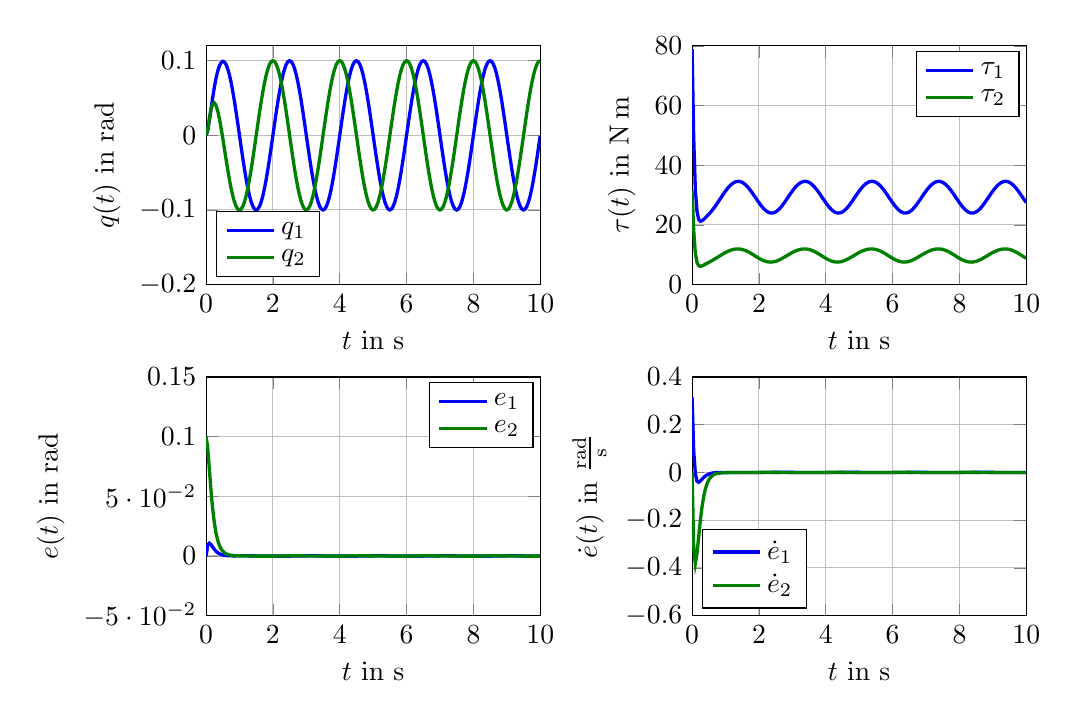
\begin{tikzpicture}

\begin{axis}[%
width=0.35\textwidth,
height=0.25\textwidth,
scale only axis,
xmin=0,
xmax=10,
xlabel={$t$ in $\mathrm{s}$},
xmajorgrids,
ymin=-0.2,
ymax=0.12,
ylabel={$q(t)$ in $\mathrm{rad}$},
ymajorgrids,
name=plot1,
legend style={at={(0.03,0.03)},anchor=south west,draw=black,fill=white,legend cell align=left}
]
\addplot [
color=blue,
solid,
line width=1.2pt
]
table[row sep=crcr]{
0 0\\
0.047 0.00580795318260061\\
0.097 0.01926381548059\\
0.147 0.0350034285292684\\
0.197 0.0504681041211654\\
0.247 0.0644468087772746\\
0.297 0.0763560323184451\\
0.347 0.0859019652849609\\
0.397 0.0929292994476793\\
0.447 0.0973584665586441\\
0.497 0.0991629879159259\\
0.547 0.0983636987555475\\
0.597 0.0950289743944933\\
0.647 0.0892760626463052\\
0.697 0.0812714667426171\\
0.747 0.0712296456862919\\
0.797 0.0594098993406237\\
0.847 0.0461115678746054\\
0.897 0.0316677826461078\\
0.947 0.0164380441037257\\
0.997 0.000799911203455122\\
1.047 -0.0148599163530817\\
1.097 -0.0301548497174351\\
1.147 -0.0447077330311305\\
1.197 -0.0581599842928409\\
1.247 -0.0701803163437733\\
1.297 -0.0804728148337447\\
1.347 -0.0887841684020454\\
1.397 -0.0949098680914763\\
1.447 -0.0986992185387737\\
1.497 -0.100059032824246\\
1.547 -0.0989559157776405\\
1.597 -0.0954170764239287\\
1.647 -0.0895296481416191\\
1.697 -0.0814385337250359\\
1.747 -0.0713428304627283\\
1.797 -0.0594909261830792\\
1.847 -0.0461743898270813\\
1.897 -0.0317208086935339\\
1.947 -0.0164857486349566\\
1.997 -0.000844033013489446\\
2.047 0.0148194488493987\\
2.097 0.0301191826569065\\
2.147 0.0446784927507786\\
2.197 0.0581388004961403\\
2.247 0.0701684532812469\\
2.297 0.0804709084914309\\
2.347 0.0887920701530265\\
2.397 0.094926594072759\\
2.447 0.0987230001725537\\
2.497 0.100087458255891\\
2.547 0.0989861454460816\\
2.597 0.0954461095673107\\
2.647 0.0895546119548269\\
2.697 0.0814569642581455\\
2.747 0.0713529149974352\\
2.797 0.059491681007972\\
2.847 0.0461657546458887\\
2.897 0.0317036483454468\\
2.947 0.0164617630319593\\
2.997 0.000815585818401063\\
3.047 -0.0148495644053689\\
3.097 -0.0301480169929354\\
3.147 -0.0447032256298006\\
3.197 -0.0581570124379221\\
3.247 -0.0701783579266379\\
3.297 -0.0804715248978078\\
3.347 -0.0887833191622952\\
3.397 -0.0949093092193569\\
3.447 -0.0986988508813461\\
3.497 -0.100058791022075\\
3.547 -0.0989557567737156\\
3.597 -0.0954169718707765\\
3.647 -0.0895295793869225\\
3.697 -0.0814384885021578\\
3.747 -0.071342800707993\\
3.797 -0.0594909065972984\\
3.847 -0.0461743769283286\\
3.897 -0.031720800193912\\
3.947 -0.0164857430308539\\
3.997 -0.000844029316374722\\
4.047 0.0148194512897485\\
4.097 0.0301191842684621\\
4.147 0.0446784938154262\\
4.197 0.0581388011996855\\
4.247 0.0701684537462539\\
4.297 0.0804709087988043\\
4.347 0.0887920703562033\\
4.397 0.0949265942070515\\
4.447 0.0987230002613055\\
4.497 0.100087458314537\\
4.547 0.0989861454848279\\
4.597 0.0954461095929064\\
4.647 0.0895546119717344\\
4.697 0.0814569642693141\\
4.747 0.0713529150048144\\
4.797 0.0594916810128496\\
4.847 0.0461657546491153\\
4.897 0.031703648347584\\
4.947 0.0164617630333774\\
4.997 0.000815585819345015\\
5.047 -0.0148495644047381\\
5.097 -0.0301480169925114\\
5.147 -0.0447032256295134\\
5.197 -0.0581570124377261\\
5.247 -0.0701783579265027\\
5.297 -0.0804715248977136\\
5.347 -0.0887833191622292\\
5.397 -0.0949093092193106\\
5.447 -0.0986988508813141\\
5.497 -0.100058791022053\\
5.547 -0.0989557567737026\\
5.597 -0.0954169718707701\\
5.647 -0.089529579386922\\
5.697 -0.0814384885021621\\
5.747 -0.0713428007080016\\
5.797 -0.0594909065973107\\
5.847 -0.046174376928344\\
5.897 -0.0317208001939302\\
5.947 -0.0164857430308739\\
5.997 -0.000844029316396397\\
6.047 0.0148194512897308\\
6.097 0.0301191842684491\\
6.147 0.0446784938154171\\
6.197 0.058138801199679\\
6.247 0.0701684537462494\\
6.297 0.0804709087988012\\
6.347 0.0887920703562012\\
6.397 0.0949265942070502\\
6.447 0.0987230002613046\\
6.497 0.100087458314537\\
6.547 0.0989861454848276\\
6.597 0.0954461095929063\\
6.647 0.0895546119717342\\
6.697 0.0814569642693141\\
6.747 0.0713529150048144\\
6.797 0.0594916810128496\\
6.847 0.0461657546491152\\
6.897 0.0317036483475837\\
6.947 0.0164617630333774\\
6.997 0.000815585819345021\\
7.047 -0.0148495644047381\\
7.097 -0.0301480169925114\\
7.147 -0.0447032256295137\\
7.197 -0.0581570124377261\\
7.247 -0.0701783579265027\\
7.297 -0.0804715248977136\\
7.347 -0.0887833191622292\\
7.397 -0.0949093092193106\\
7.447 -0.0986988508813141\\
7.497 -0.100058791022053\\
7.547 -0.0989557567737026\\
7.597 -0.0954169718707701\\
7.647 -0.0895295793869218\\
7.697 -0.0814384885021621\\
7.747 -0.0713428007080017\\
7.797 -0.0594909065973107\\
7.847 -0.046174376928344\\
7.897 -0.03172080019393\\
7.947 -0.0164857430308739\\
7.997 -0.000844029316396429\\
8.047 0.0148194512897407\\
8.097 0.0301191842684689\\
8.147 0.044678493815444\\
8.197 0.0581388011997096\\
8.247 0.0701684537462816\\
8.297 0.0804709087988327\\
8.347 0.0887920703562298\\
8.397 0.0949265942070748\\
8.447 0.098723000261324\\
8.497 0.10008745831455\\
8.547 0.0989861454848343\\
8.597 0.095446109592906\\
8.647 0.0895546119717269\\
8.697 0.0814569642693\\
8.747 0.0713529150047936\\
8.797 0.0594916810128224\\
8.847 0.0461657546490828\\
8.897 0.0317036483475465\\
8.947 0.0164617630333367\\
8.997 0.000815585819301244\\
9.047 -0.0148495644047838\\
9.097 -0.0301480169925575\\
9.147 -0.0447032256295592\\
9.197 -0.0581570124377698\\
9.247 -0.0701783579265439\\
9.297 -0.0804715248977512\\
9.347 -0.0887833191622619\\
9.397 -0.0949093092193379\\
9.447 -0.0986988508813352\\
9.497 -0.100058791022068\\
9.547 -0.0989557567737101\\
9.597 -0.0954169718707705\\
9.647 -0.089529579386915\\
9.697 -0.0814384885021484\\
9.747 -0.0713428007079811\\
9.797 -0.0594909065972837\\
9.847 -0.0461743769283117\\
9.897 -0.031720800193893\\
9.947 -0.0164857430308334\\
9.997 -0.000844029316352776\\
};
\addlegendentry{$q_1$};

\addplot [
color=green!50!black,
solid,
line width=1.2pt
]
table[row sep=crcr]{
0 0\\
0.047 0.007682416078996\\
0.097 0.0222542703420776\\
0.147 0.0346414439230778\\
0.197 0.0418478269455009\\
0.247 0.0435018118223462\\
0.297 0.0402453668130583\\
0.347 0.0330262624071445\\
0.397 0.022809542962661\\
0.447 0.0104767382742467\\
0.497 -0.00319619506669238\\
0.547 -0.0175321421701998\\
0.597 -0.031938990263358\\
0.647 -0.0458971263415413\\
0.697 -0.0589507696921401\\
0.747 -0.0707031649037316\\
0.797 -0.0808147911496111\\
0.847 -0.0890035698177099\\
0.897 -0.0950461491858836\\
0.947 -0.0987795213243837\\
0.997 -0.100102404809714\\
1.047 -0.0989759809583492\\
1.097 -0.0954236970426772\\
1.147 -0.0895299513178355\\
1.197 -0.0814375574377234\\
1.247 -0.0713439550184704\\
1.297 -0.0594961922924373\\
1.347 -0.046184758090011\\
1.397 -0.0317363846975987\\
1.447 -0.0165059805264181\\
1.497 -0.000867881563937192\\
1.547 0.0147933672632459\\
1.597 0.0300924756995687\\
1.647 0.0446528856089504\\
1.697 0.0581160323088128\\
1.747 0.0701501670371885\\
1.797 0.0804585297305437\\
1.847 0.0887866769007761\\
1.897 0.0949287881063256\\
1.947 0.0987327962091631\\
1.997 0.100104211492434\\
2.047 0.0990085380095442\\
2.097 0.0954722122664991\\
2.147 0.0895820292048845\\
2.197 0.0814830578388101\\
2.247 0.0713750879566113\\
2.297 0.0595076890131631\\
2.347 0.0461740015342861\\
2.397 0.0317034186251038\\
2.447 0.0164533488158442\\
2.497 0.000800279523445711\\
2.547 -0.0148696191540333\\
2.597 -0.0301700993951566\\
2.647 -0.044724397262369\\
2.697 -0.0581745072360169\\
2.747 -0.0701899422393908\\
2.797 -0.0804757734422534\\
2.847 -0.0887797686952464\\
2.897 -0.0948984738302396\\
2.947 -0.0986821062366936\\
2.997 -0.100038155092668\\
3.047 -0.0989336081016178\\
3.097 -0.0953957515024223\\
3.147 -0.0895115192086144\\
3.197 -0.0814253984350482\\
3.247 -0.0713359327540326\\
3.297 -0.0594908983321964\\
3.347 -0.046181263869318\\
3.397 -0.0317340779510037\\
3.447 -0.0165044574691109\\
3.497 -0.000866875837414025\\
3.547 0.0147940314130247\\
3.597 0.030092914276621\\
3.647 0.0446531752023401\\
3.697 0.0581162234979234\\
3.747 0.070150293231582\\
3.797 0.0804586130015005\\
3.847 0.0887867318299326\\
3.897 0.0949288243267678\\
3.947 0.0987328200838966\\
3.997 0.100104227223456\\
4.047 0.0990085483708745\\
4.097 0.0954722190887383\\
4.147 0.0895820336955313\\
4.197 0.0814830607939817\\
4.247 0.0713750899009502\\
4.297 0.0595076902922526\\
4.347 0.0461740023756686\\
4.397 0.0317034191785453\\
4.447 0.0164533491798891\\
4.497 0.000800279762921375\\
4.547 -0.0148696189964883\\
4.597 -0.0301700992914998\\
4.647 -0.0447243971941583\\
4.697 -0.0581745071911244\\
4.747 -0.0701899422098394\\
4.797 -0.0804757734227969\\
4.847 -0.0887797686824337\\
4.897 -0.0948984738218005\\
4.947 -0.0986821062311345\\
4.997 -0.100038155089006\\
5.047 -0.0989336080992062\\
5.097 -0.0953957515008353\\
5.147 -0.0895115192075718\\
5.197 -0.0814253984343655\\
5.247 -0.0713359327535881\\
5.297 -0.0594908983319098\\
5.347 -0.0461812638691362\\
5.397 -0.0317340779508918\\
5.447 -0.016504457469045\\
5.497 -0.000866875837378996\\
5.547 0.0147940314130395\\
5.597 0.0300929142766228\\
5.647 0.0446531752023335\\
5.697 0.0581162234979123\\
5.747 0.0701502932315685\\
5.797 0.0804586130014865\\
5.847 0.0887867318299193\\
5.897 0.0949288243267562\\
5.947 0.0987328200838873\\
5.997 0.10010422722345\\
6.047 0.0990085483708707\\
6.097 0.095472219088736\\
6.147 0.0895820336955298\\
6.197 0.0814830607939808\\
6.247 0.0713750899009497\\
6.297 0.0595076902922524\\
6.347 0.0461740023756684\\
6.397 0.0317034191785449\\
6.447 0.0164533491798891\\
6.497 0.000800279762921352\\
6.547 -0.0148696189964883\\
6.597 -0.0301700992914999\\
6.647 -0.0447243971941586\\
6.697 -0.0581745071911244\\
6.747 -0.0701899422098394\\
6.797 -0.0804757734227969\\
6.847 -0.0887797686824337\\
6.897 -0.0948984738218005\\
6.947 -0.0986821062311345\\
6.997 -0.100038155089006\\
7.047 -0.0989336080992062\\
7.097 -0.0953957515008353\\
7.147 -0.0895115192075717\\
7.197 -0.0814253984343655\\
7.247 -0.0713359327535881\\
7.297 -0.0594908983319098\\
7.347 -0.0461812638691363\\
7.397 -0.0317340779508915\\
7.447 -0.016504457469045\\
7.497 -0.000866875837378987\\
7.547 0.0147940314130396\\
7.597 0.0300929142766228\\
7.647 0.0446531752023338\\
7.697 0.0581162234979123\\
7.747 0.0701502932315685\\
7.797 0.0804586130014865\\
7.847 0.0887867318299193\\
7.897 0.0949288243267563\\
7.947 0.0987328200838873\\
7.997 0.10010422722345\\
8.047 0.0990085483708693\\
8.097 0.0954722190887309\\
8.147 0.0895820336955195\\
8.197 0.0814830607939649\\
8.247 0.0713750899009277\\
8.297 0.0595076902922244\\
8.347 0.0461740023756355\\
8.397 0.0317034191785074\\
8.447 0.0164533491798482\\
8.497 0.000800279762877432\\
8.547 -0.0148696189965342\\
8.597 -0.030170099291546\\
8.647 -0.0447243971942042\\
8.697 -0.0581745071911681\\
8.747 -0.0701899422098806\\
8.797 -0.0804757734228345\\
8.847 -0.0887797686824666\\
8.897 -0.0948984738218279\\
8.947 -0.0986821062311556\\
8.997 -0.100038155089021\\
9.047 -0.0989336080992136\\
9.097 -0.0953957515008355\\
9.147 -0.0895115192075648\\
9.197 -0.0814253984343516\\
9.247 -0.0713359327535674\\
9.297 -0.0594908983318827\\
9.347 -0.0461812638691039\\
9.397 -0.0317340779508544\\
9.447 -0.0165044574690044\\
9.497 -0.000866875837335279\\
9.547 0.0147940314130853\\
9.597 0.0300929142766689\\
9.647 0.0446531752023794\\
9.697 0.058116223497956\\
9.747 0.0701502932316098\\
9.797 0.0804586130015242\\
9.847 0.0887867318299521\\
9.897 0.0949288243267836\\
9.947 0.0987328200839085\\
9.997 0.100104227223464\\
};
\addlegendentry{$q_2$};

\end{axis}

\begin{axis}[%
width=0.35\textwidth,
height=0.25\textwidth,
scale only axis,
xmin=0,
xmax=10,
xlabel={$t$ in $\mathrm{s}$},
xmajorgrids,
ymin=-0.05,
ymax=0.15,
ylabel={$e(t)$ in $\mathrm{rad}$},
ymajorgrids,
name=plot3,
at=(plot1.below south west),
anchor=above north west,
legend style={draw=black,fill=white,legend cell align=left}
]
\addplot [
color=blue,
solid,
line width=1.2pt
]
table[row sep=crcr]{
0 0\\
0.047 0.00890393800126314\\
0.097 0.0107401751435376\\
0.147 0.00955386370842119\\
0.197 0.00754534131801955\\
0.247 0.00559430630110601\\
0.297 0.00398810769276763\\
0.347 0.00276686028509476\\
0.397 0.00188089092072391\\
0.447 0.00125854706425481\\
0.497 0.000832570794969095\\
0.547 0.000548182521648705\\
0.597 0.000363690662246008\\
0.647 0.000248502186175989\\
0.697 0.000180605964433866\\
0.747 0.000144314541350277\\
0.797 0.000128484630211756\\
0.847 0.000125207229493739\\
0.897 0.000128880737133297\\
0.947 0.000135568179086241\\
0.997 0.000142552639859277\\
1.047 0.000148025169218202\\
1.097 0.000150859093307722\\
1.147 0.000150440793441058\\
1.197 0.000146538853656217\\
1.247 0.00013920126539288\\
1.297 0.000128674822532107\\
1.347 0.000115342831989815\\
1.397 9.96777230731216e-05\\
1.447 8.22049158748783e-05\\
1.497 6.34741133505312e-05\\
1.547 4.40345004442677e-05\\
1.597 2.44113671893087e-05\\
1.647 5.08330913778776e-06\\
1.697 -1.35389820152543e-05\\
1.747 -3.11297649139702e-05\\
1.797 -4.7457787756465e-05\\
1.847 -6.23852770180733e-05\\
1.897 -7.58546897073956e-05\\
1.947 -8.78636478557106e-05\\
1.997 -9.84308298251868e-05\\
2.047 -0.000107557665535231\\
2.097 -0.0001151920327792\\
2.147 -0.000121200513089212\\
2.197 -0.000125355056955614\\
2.247 -0.00012733820286645\\
2.297 -0.00012676848021824\\
2.347 -0.000123244582970958\\
2.397 -0.000116403704355852\\
2.447 -0.000105986549654866\\
2.497 -9.18995449964294e-05\\
2.547 -7.42641688853546e-05\\
2.597 -5.34445105711961e-05\\
2.647 -3.00471223456666e-05\\
2.697 -4.89155109438533e-06\\
2.747 2.10452302070729e-05\\
2.797 4.67029628637705e-05\\
2.847 7.10204582106896e-05\\
2.897 9.30150377944639e-05\\
2.947 0.000111849250852909\\
2.997 0.000126878024913493\\
3.047 0.000137673221505433\\
3.097 0.000144026368808132\\
3.147 0.000145933392111233\\
3.197 0.000143566998737438\\
3.247 0.000137242848257474\\
3.297 0.000127384886595222\\
3.347 0.000114493592239709\\
3.397 9.91188509537749e-05\\
3.447 8.18372584472787e-05\\
3.497 6.32323111798422e-05\\
3.547 4.38754965194077e-05\\
3.597 2.43068140369923e-05\\
3.647 5.01455444119892e-06\\
3.697 -1.35842048933077e-05\\
3.747 -3.11595196492848e-05\\
3.797 -4.74773735373996e-05\\
3.847 -6.23981757708406e-05\\
3.897 -7.58631893292352e-05\\
3.947 -8.78692519583509e-05\\
3.997 -9.84345269398468e-05\\
4.047 -0.000107560105884173\\
4.097 -0.000115193644333805\\
4.147 -0.00012120157773602\\
4.197 -0.000125355760499983\\
4.247 -0.00012733866787272\\
4.297 -0.000126768787591089\\
4.347 -0.000123244786147336\\
4.397 -0.000116403838648166\\
4.447 -0.000105986638406483\\
4.497 -9.18996036422537e-05\\
4.547 -7.42642076317773e-05\\
4.597 -5.34445361673047e-05\\
4.647 -3.00471392535168e-05\\
4.697 -4.89156226356202e-06\\
4.747 2.10452228271429e-05\\
4.797 4.67029579853256e-05\\
4.847 7.10204549833754e-05\\
4.897 9.30150356565698e-05\\
4.947 0.000111849249433742\\
4.997 0.000126878023968678\\
5.047 0.000137673220873717\\
5.097 0.000144026368383107\\
5.147 0.000145933391823401\\
5.197 0.000143566998540484\\
5.247 0.000137242848121638\\
5.297 0.000127384886500395\\
5.347 0.000114493592173165\\
5.397 9.91188509071872e-05\\
5.447 8.18372584150684e-05\\
5.497 6.32323111584288e-05\\
5.547 4.38754965065014e-05\\
5.597 2.43068140309e-05\\
5.647 5.01455444106014e-06\\
5.697 -1.35842048884782e-05\\
5.747 -3.1159519639945e-05\\
5.797 -4.74773735243891e-05\\
5.847 -6.23981757546174e-05\\
5.897 -7.58631893101949e-05\\
5.947 -8.78692519373087e-05\\
5.997 -9.84345269171303e-05\\
6.047 -0.000107560105866444\\
6.097 -0.00011519364432077\\
6.147 -0.000121201577726819\\
6.197 -0.000125355760493343\\
6.247 -0.000127338667868376\\
6.297 -0.000126768787588022\\
6.347 -0.000123244786145144\\
6.397 -0.000116403838646709\\
6.447 -0.000105986638405636\\
6.497 -9.18996036416569e-05\\
6.547 -7.42642076314859e-05\\
6.597 -5.34445361670827e-05\\
6.647 -3.00471392534335e-05\\
6.697 -4.89156226350651e-06\\
6.747 2.10452228271985e-05\\
6.797 4.67029579855199e-05\\
6.847 7.10204549834101e-05\\
6.897 9.30150356567017e-05\\
6.947 0.000111849249433776\\
6.997 0.000126878023968519\\
7.047 0.000137673220873732\\
7.097 0.000144026368383135\\
7.147 0.000145933391823366\\
7.197 0.000143566998540498\\
7.247 0.000137242848121666\\
7.297 0.000127384886500409\\
7.347 0.000114493592173165\\
7.397 9.91188509071733e-05\\
7.447 8.18372584150684e-05\\
7.497 6.32323111584288e-05\\
7.547 4.38754965065152e-05\\
7.597 2.43068140309e-05\\
7.647 5.01455444107402e-06\\
7.697 -1.35842048884505e-05\\
7.747 -3.1159519639945e-05\\
7.797 -4.74773735243822e-05\\
7.847 -6.23981757546174e-05\\
7.897 -7.58631893104655e-05\\
7.947 -8.78692519373087e-05\\
7.997 -9.84345269171225e-05\\
8.047 -0.000107560105878176\\
8.097 -0.00011519364434262\\
8.147 -0.000121201577755276\\
8.197 -0.000125355760526004\\
8.247 -0.00012733866790185\\
8.297 -0.000126768787620565\\
8.347 -0.000123244786174828\\
8.397 -0.000116403838671994\\
8.447 -0.000105986638425329\\
8.497 -9.18996036550629e-05\\
8.547 -7.42642076379529e-05\\
8.597 -5.34445361662916e-05\\
8.647 -3.0047139245204e-05\\
8.697 -4.89156224822707e-06\\
8.747 2.10452228495001e-05\\
8.797 4.67029580138653e-05\\
8.847 7.1020455017487e-05\\
8.897 9.3015035695615e-05\\
8.947 0.000111849249476617\\
8.997 0.000126878024014452\\
9.047 0.000137673220921284\\
9.097 0.000144026368431281\\
9.147 0.00014593339187053\\
9.197 0.000143566998586218\\
9.247 0.000137242848164132\\
9.297 0.000127384886539059\\
9.347 0.000114493592206916\\
9.397 9.91188509351371e-05\\
9.447 8.18372584366067e-05\\
9.497 6.32323111730282e-05\\
9.547 4.38754965138149e-05\\
9.597 2.43068140308028e-05\\
9.647 5.01455443333021e-06\\
9.697 -1.35842049033691e-05\\
9.747 -3.11595196620384e-05\\
9.797 -4.7477373552568e-05\\
9.847 -6.23981757885139e-05\\
9.897 -7.58631893491776e-05\\
9.947 -8.78692519799794e-05\\
9.997 -9.84345269629323e-05\\
};
\addlegendentry{$e_1$};

\addplot [
color=green!50!black,
solid,
line width=1.2pt
]
table[row sep=crcr]{
0 0.1\\
0.047 0.0912294651982002\\
0.097 0.0731383947146618\\
0.147 0.0548831209094034\\
0.197 0.03960424576155\\
0.247 0.0278721484052959\\
0.297 0.0192930171577772\\
0.347 0.0132105126969546\\
0.397 0.00898712042058007\\
0.447 0.00609687400856526\\
0.497 0.0041386589100068\\
0.547 0.0028202509863361\\
0.597 0.00193499963923041\\
0.647 0.00133983410385167\\
0.697 0.000937324252955139\\
0.747 0.000662049825350966\\
0.797 0.000470651138398365\\
0.847 0.000334744247654284\\
0.897 0.000235958817480411\\
0.947 0.000162507701484765\\
0.997 0.000106846098819086\\
1.047 6.40996811529654e-05\\
1.097 3.10319859377767e-05\\
1.147 5.38648535421127e-06\\
1.197 -1.45152693277056e-05\\
1.247 -3.00052091719433e-05\\
1.297 -4.21916783984178e-05\\
1.347 -5.20170140884124e-05\\
1.397 -6.02786856426368e-05\\
1.447 -6.7631756394182e-05\\
1.497 -7.45822793774347e-05\\
1.547 -8.14760793824056e-05\\
1.597 -8.84850754412601e-05\\
1.647 -9.55933712609436e-05\\
1.697 -0.000102586869628163\\
1.747 -0.00010905195880806\\
1.797 -0.000114389719331115\\
1.847 -0.000117851330720536\\
1.897 -0.000118597737922471\\
1.947 -0.000115782586264296\\
1.997 -0.000108652781539029\\
2.047 -9.66567323479883e-05\\
2.097 -7.95472097596533e-05\\
2.147 -5.74643724032403e-05\\
2.197 -3.09851317589899e-05\\
2.247 -1.12772896902757e-06\\
2.297 3.06949576726195e-05\\
2.347 6.27735698133652e-05\\
2.397 9.32447581375243e-05\\
2.447 0.000120263466968102\\
2.497 0.000142184319868928\\
2.547 0.000157727970169837\\
2.597 0.000166108771029336\\
2.647 0.000167105024679565\\
2.697 0.000161061796832195\\
2.747 0.000148827161010293\\
2.797 0.00013163343104082\\
2.847 0.000110943125190846\\
2.897 8.82834618364386e-05\\
2.947 6.50926137947538e-05\\
2.997 4.25963817731606e-05\\
3.047 2.17268244215862e-05\\
3.097 3.08644568279559e-06\\
3.147 -1.30456238669197e-05\\
3.197 -2.66742720028967e-05\\
3.247 -3.80274736096614e-05\\
3.297 -4.74856386393774e-05\\
3.347 -5.55112347813552e-05\\
3.397 -6.25854322375483e-05\\
3.447 -6.9154813701313e-05\\
3.497 -7.55880059005381e-05\\
3.547 -8.21402291612313e-05\\
3.597 -8.89236524937442e-05\\
3.647 -9.58829646506773e-05\\
3.697 -0.000102778058738699\\
3.747 -0.000109178153201536\\
3.797 -0.000114472990287953\\
3.847 -0.000117906259877024\\
3.897 -0.0001186339583647\\
3.947 -0.00011580646099775\\
3.997 -0.000108668512561236\\
4.047 -9.66670936784347e-05\\
4.097 -7.95540319992183e-05\\
4.147 -5.74688630504139e-05\\
4.197 -3.09880869311385e-05\\
4.247 -1.12967330864744e-06\\
4.297 3.06936785822928e-05\\
4.347 6.27727284300619e-05\\
4.397 9.32442046953225e-05\\
4.447 0.000120263102922038\\
4.497 0.000142184080392311\\
4.547 0.000157727812623923\\
4.597 0.000166108667371535\\
4.647 0.000167104956468142\\
4.697 0.000161061751938842\\
4.747 0.000148827131458237\\
4.797 0.000131633411583718\\
4.847 0.000110943112377804\\
4.897 8.82834533971061e-05\\
4.947 6.50926082355202e-05\\
4.997 4.25963781111871e-05\\
5.047 2.17268220100708e-05\\
5.097 3.08644409614811e-06\\
5.147 -1.30456249091276e-05\\
5.197 -2.66742726849623e-05\\
5.247 -3.80274740536257e-05\\
5.297 -4.74856389251696e-05\\
5.347 -5.55112349622244e-05\\
5.397 -6.25854323488412e-05\\
5.447 -6.91548137663478e-05\\
5.497 -7.55880059347029e-05\\
5.547 -8.21402291750241e-05\\
5.597 -8.89236524946706e-05\\
5.647 -9.58829646433637e-05\\
5.697 -0.000102778058726806\\
5.747 -0.000109178153187339\\
5.797 -0.000114472990273479\\
5.847 -0.000117906259863382\\
5.897 -0.000118633958352779\\
5.947 -0.000115806460988327\\
5.997 -0.000108668512554796\\
6.047 -9.66670936746045e-05\\
6.097 -7.95540319968868e-05\\
6.147 -5.74688630489567e-05\\
6.197 -3.09880869303614e-05\\
6.247 -1.12967330799518e-06\\
6.297 3.06936785825565e-05\\
6.347 6.27727284300481e-05\\
6.397 9.32442046953433e-05\\
6.447 0.000120263102922277\\
6.497 0.000142184080392359\\
6.547 0.0001577278126238\\
6.597 0.000166108667371757\\
6.647 0.000167104956468107\\
6.697 0.000161061751938862\\
6.747 0.000148827131458237\\
6.797 0.000131633411583801\\
6.847 0.000110943112377776\\
6.897 8.82834533971338e-05\\
6.947 6.50926082355063e-05\\
6.997 4.25963781111732e-05\\
7.047 2.17268220100708e-05\\
7.097 3.08644409614811e-06\\
7.147 -1.30456249091138e-05\\
7.197 -2.66742726849623e-05\\
7.247 -3.80274740536535e-05\\
7.297 -4.74856389251974e-05\\
7.347 -5.55112349622452e-05\\
7.397 -6.25854323487857e-05\\
7.447 -6.91548137663721e-05\\
7.497 -7.5588005934736e-05\\
7.547 -8.2140229175057e-05\\
7.597 -8.89236524946949e-05\\
7.647 -9.58829646433221e-05\\
7.697 -0.000102778058726834\\
7.747 -0.000109178153187367\\
7.797 -0.000114472990273465\\
7.847 -0.000117906259863354\\
7.897 -0.000118633958352862\\
7.947 -0.000115806460988285\\
7.997 -0.000108668512554769\\
8.047 -9.66670936729808e-05\\
8.097 -7.95540319911414e-05\\
8.147 -5.74688630378822e-05\\
8.197 -3.09880869130558e-05\\
8.247 -1.12967328476377e-06\\
8.297 3.06936786119497e-05\\
8.347 6.27727284649091e-05\\
8.397 9.3244204734895e-05\\
8.447 0.000120263102965337\\
8.497 0.00014218408043808\\
8.547 0.000157727812671432\\
8.597 0.000166108667419625\\
8.647 0.000167104956515667\\
8.697 0.00016106175198434\\
8.747 0.000148827131500981\\
8.797 0.000131633411622298\\
8.847 0.000110943112411457\\
8.897 8.82834534250421e-05\\
8.947 6.50926082569614e-05\\
8.997 4.25963781257171e-05\\
9.047 2.17268220172456e-05\\
9.097 3.08644409573178e-06\\
9.147 -1.30456249168021e-05\\
9.197 -2.66742727002556e-05\\
9.247 -3.80274740755526e-05\\
9.297 -4.74856389537093e-05\\
9.347 -5.55112349965303e-05\\
9.397 -6.25854323879349e-05\\
9.447 -6.91548138091296e-05\\
9.497 -7.55880059802454e-05\\
9.547 -8.21402292225659e-05\\
9.597 -8.892365254249e-05\\
9.647 -9.58829646908119e-05\\
9.697 -0.000102778058772304\\
9.747 -0.000109178153230138\\
9.797 -0.000114472990312017\\
9.847 -0.000117906259897035\\
9.897 -0.000118633958380784\\
9.947 -0.000115806461009824\\
9.997 -0.000108668512569313\\
};
\addlegendentry{$e_2$};

\end{axis}

\begin{axis}[%
width=0.35\textwidth,
height=0.25\textwidth,
scale only axis,
xmin=0,
xmax=10,
xlabel={$t$ in $\mathrm{s}$},
xmajorgrids,
ymin=-0.6,
ymax=0.4,
ylabel={$\dot{e}(t)$ in $\mathrm{\frac{rad}{s}}$},
ymajorgrids,
name=plot2,
at=(plot3.right of south east),
anchor=left of south west,
legend style={at={(0.03,0.03)},anchor=south west,draw=black,fill=white,legend cell align=left}
]
\addplot [
color=blue,
solid,
line width=1.2pt
]
table[row sep=crcr]{
0 0.314159265358979\\
0.047 0.0935519453955888\\
0.097 -0.00410100838646821\\
0.147 -0.0363817139318284\\
0.197 -0.0412053977590386\\
0.247 -0.0359620917442832\\
0.297 -0.0281886502194724\\
0.347 -0.0208404235727135\\
0.397 -0.0148405086910546\\
0.447 -0.0102769675339551\\
0.497 -0.00694377067803594\\
0.547 -0.00457109147639244\\
0.597 -0.00291302003352639\\
0.647 -0.00177277821969607\\
0.697 -0.0010026955013501\\
0.747 -0.000495693978657674\\
0.797 -0.000175379957720101\\
0.847 1.25915567912305e-05\\
0.897 0.000107169281754305\\
0.947 0.000136667368980881\\
0.997 0.000122005212196963\\
1.047 7.88386587435852e-05\\
1.097 1.89451429427057e-05\\
1.147 -4.88575805203673e-05\\
1.197 -0.000118064939008733\\
1.247 -0.000183991804633715\\
1.297 -0.000243370120462771\\
1.347 -0.000294016163149502\\
1.397 -0.000334567467364863\\
1.447 -0.000364295406487823\\
1.497 -0.000382993265804695\\
1.547 -0.000390926480831902\\
1.597 -0.000388817675121417\\
1.647 -0.0003778302421521\\
1.697 -0.000359514791552551\\
1.747 -0.000335693987488422\\
1.797 -0.000308280647929149\\
1.847 -0.000279046117212522\\
1.897 -0.000249374624328891\\
1.947 -0.000220049593779637\\
1.997 -0.000191117401769025\\
2.047 -0.000161863577965882\\
2.097 -0.000130918833228966\\
2.147 -9.64912991757716e-05\\
2.197 -5.67004606402688e-05\\
2.247 -9.97008948028233e-06\\
2.297 4.45759914173005e-05\\
2.347 0.000106778486497094\\
2.397 0.000175229275009708\\
2.447 0.000247230068157807\\
2.497 0.000318950099226161\\
2.547 0.000385777547201607\\
2.597 0.000442822850313107\\
2.647 0.000485499493827868\\
2.697 0.000510088267184794\\
2.747 0.000514190942161291\\
2.797 0.00049700010026027\\
2.847 0.00045934850472229\\
2.897 0.000403544416828883\\
2.947 0.000333037752479615\\
2.997 0.000251987350109784\\
3.047 0.000164807747364659\\
3.097 7.57654623233517e-05\\
3.147 -1.13257875758443e-05\\
3.197 -9.32881036855848e-05\\
3.247 -0.000167644366790565\\
3.297 -0.000232590291552232\\
3.347 -0.000286911684342056\\
3.397 -0.000329887816064925\\
3.447 -0.000361214598249476\\
3.497 -0.000380966033149554\\
3.547 -0.000389593086498594\\
3.597 -0.000387940938803358\\
3.647 -0.000377253894838725\\
3.697 -0.00035913594602055\\
3.747 -0.000335444949500135\\
3.797 -0.000308116906427514\\
3.847 -0.000278938420401109\\
3.897 -0.000249303756095387\\
3.947 -0.000220002933474739\\
3.997 -0.000191086660699058\\
4.047 -0.000161843311511312\\
4.097 -0.000130905463605058\\
4.147 -9.64824740021797e-05\\
4.197 -5.66946321408079e-05\\
4.247 -9.96623845428424e-06\\
4.297 4.45785366834928e-05\\
4.347 0.000106780169077531\\
4.397 0.000175230387395725\\
4.447 0.000247230803566874\\
4.497 0.000318950585367255\\
4.547 0.000385777868517664\\
4.597 0.000442823062651129\\
4.647 0.000485499634127473\\
4.697 0.000510088359876232\\
4.747 0.000514191003398584\\
4.797 0.000497000140723458\\
4.847 0.000459348531469783\\
4.897 0.000403544434522618\\
4.947 0.000333037764199295\\
4.997 0.000251987357888173\\
5.047 0.000164807752542517\\
5.097 7.57654657853046e-05\\
5.147 -1.1325785247096e-05\\
5.197 -9.32881021054044e-05\\
5.247 -0.000167644365708319\\
5.297 -0.000232590290801526\\
5.347 -0.000286911683814645\\
5.397 -0.000329887815690572\\
5.447 -0.000361214597982377\\
5.497 -0.000380966032958574\\
5.547 -0.000389593086364506\\
5.597 -0.000387940938714804\\
5.647 -0.000377253894786295\\
5.697 -0.000359135945999789\\
5.747 -0.000335444949506519\\
5.797 -0.0003081169064586\\
5.847 -0.000278938420453789\\
5.897 -0.000249303756166497\\
5.947 -0.000220002933562169\\
5.997 -0.000191086660799977\\
6.047 -0.000161843311612786\\
6.097 -0.000130905463689934\\
6.147 -9.64824740671832e-05\\
6.197 -5.66946321890471e-05\\
6.247 -9.96623848784073e-06\\
6.297 4.45785366597895e-05\\
6.347 0.000106780169060655\\
6.397 0.000175230387384331\\
6.447 0.000247230803559886\\
6.497 0.000318950585362205\\
6.547 0.000385777868513924\\
6.597 0.000442823062649964\\
6.647 0.000485499634126363\\
6.697 0.00051008835987551\\
6.747 0.000514191003398196\\
6.797 0.00049700014072368\\
6.847 0.000459348531469617\\
6.897 0.000403544434522729\\
6.947 0.000333037764199351\\
6.997 0.000251987357888006\\
7.047 0.000164807752542462\\
7.097 7.57654657854157e-05\\
7.147 -1.13257852470405e-05\\
7.197 -9.32881021054599e-05\\
7.247 -0.000167644365708541\\
7.297 -0.000232590290801665\\
7.347 -0.000286911683814783\\
7.397 -0.000329887815690377\\
7.447 -0.000361214597982364\\
7.497 -0.000380966032958602\\
7.547 -0.000389593086364583\\
7.597 -0.000387940938714873\\
7.647 -0.000377253894786073\\
7.697 -0.000359135945999622\\
7.747 -0.000335444949506603\\
7.797 -0.000308116906458766\\
7.847 -0.0002789384204539\\
7.897 -0.000249303756166608\\
7.947 -0.000220002933562058\\
7.997 -0.000191086660799866\\
8.047 -0.000161843311592191\\
8.097 -0.000130905463620601\\
8.147 -9.64824739497216e-05\\
8.197 -5.66946320328943e-05\\
8.247 -9.96623830851195e-06\\
8.297 4.45785368507756e-05\\
8.347 0.000106780169251253\\
8.397 0.000175230387564507\\
8.447 0.000247230803720522\\
8.497 0.000318950585497379\\
8.547 0.000385777868619638\\
8.597 0.00044282306272006\\
8.647 0.000485499634160058\\
8.697 0.000510088359870209\\
8.747 0.000514191003355008\\
8.797 0.000497000140641524\\
8.847 0.0004593485313516\\
8.897 0.000403544434371295\\
8.947 0.000333037764018218\\
8.997 0.000251987357682004\\
9.047 0.000164807752316254\\
9.097 7.57654655442197e-05\\
9.147 -1.13257854963411e-05\\
9.197 -9.32881023579801e-05\\
9.247 -0.000167644365956315\\
9.297 -0.000232590291040474\\
9.347 -0.000286911684037994\\
9.397 -0.000329887815892813\\
9.447 -0.000361214598157883\\
9.497 -0.000380966033103456\\
9.547 -0.000389593086476785\\
9.597 -0.000387940938789577\\
9.647 -0.000377253894823265\\
9.697 -0.000359135945996902\\
9.747 -0.000335444949465025\\
9.797 -0.000308116906377665\\
9.847 -0.00027893842033655\\
9.897 -0.000249303756016062\\
9.947 -0.000220002933382091\\
9.997 -0.000191086660594753\\
};
\addlegendentry{$\dot{e}_1$};

\addplot [
color=green!50!black,
solid,
line width=1.2pt
]
table[row sep=crcr]{
0 -0\\
0.047 -0.31414212673186\\
0.097 -0.380703685107415\\
0.147 -0.339987528519918\\
0.197 -0.269731785872251\\
0.247 -0.201093926670776\\
0.297 -0.14437436488422\\
0.347 -0.101112152723266\\
0.397 -0.0696130353431838\\
0.447 -0.0473587493494214\\
0.497 -0.0319634791670271\\
0.547 -0.0214782839233666\\
0.597 -0.0144230686571891\\
0.647 -0.00972053427334868\\
0.697 -0.0066078010867732\\
0.747 -0.00455511944168829\\
0.797 -0.00320039177986622\\
0.847 -0.00229974609465119\\
0.897 -0.00169151328691147\\
0.947 -0.0012704692201437\\
0.997 -0.000969602356545059\\
1.047 -0.000747290369490394\\
1.097 -0.000578346181522485\\
1.147 -0.000447843243551849\\
1.197 -0.000346948671497704\\
1.247 -0.000270206667526168\\
1.297 -0.000213854690872817\\
1.347 -0.000174849000411426\\
1.397 -0.000150346238432186\\
1.447 -0.000137448627379799\\
1.497 -0.0001330799827996\\
1.547 -0.000133918908416408\\
1.597 -0.000136369028009176\\
1.647 -0.00013658545674855\\
1.697 -0.000130594311123278\\
1.747 -0.000114535192123039\\
1.797 -8.50295308975901e-05\\
1.847 -3.96407282321487e-05\\
1.897 2.26422264583137e-05\\
1.947 0.000100986947556642\\
1.997 0.000192457263132368\\
2.047 0.000291985850212097\\
2.097 0.000392625588264972\\
2.147 0.0004860872840175\\
2.197 0.000563530348723029\\
2.247 0.000616532697240768\\
2.297 0.00063812998091195\\
2.347 0.000623786808879312\\
2.397 0.000572150437215868\\
2.447 0.000485448187142967\\
2.497 0.000369429271389943\\
2.547 0.000232819229145087\\
2.597 8.63409477532828e-05\\
2.647 -5.85584512112214e-05\\
2.697 -0.000191073405644948\\
2.747 -0.000302276404363533\\
2.797 -0.000386031314206586\\
2.847 -0.0004394588464261\\
2.897 -0.00046292037313031\\
2.947 -0.000459575219696029\\
2.997 -0.000434633356335785\\
3.047 -0.000394458920877562\\
3.097 -0.000345679155817152\\
3.147 -0.000294424836030788\\
3.197 -0.000245782750296131\\
3.247 -0.000203489494107256\\
3.297 -0.000169848520475635\\
3.347 -0.000145816730952542\\
3.397 -0.000131188191064224\\
3.447 -0.000124803371764848\\
3.497 -0.00012473155045728\\
3.547 -0.000128406140947779\\
3.597 -0.000132728196932885\\
3.647 -0.000134180708936615\\
3.697 -0.00012900597010379\\
3.747 -0.000113486163559301\\
3.797 -8.43368012212742e-05\\
3.847 -3.9183388877595e-05\\
3.897 2.29440694456823e-05\\
3.947 0.000101186091321717\\
3.997 0.000192588597432483\\
4.047 0.000292072427958381\\
4.097 0.000392682637578995\\
4.147 0.000486124860660214\\
4.197 0.000563555090073165\\
4.247 0.000616548982209891\\
4.297 0.00063814069692103\\
4.347 0.000623793858871458\\
4.397 0.000572155074685887\\
4.447 0.0004854512374039\\
4.497 0.000369431277620347\\
4.547 0.000232820548719925\\
4.597 8.63418157435736e-05\\
4.647 -5.85578802081432e-05\\
4.697 -0.000191073029965294\\
4.747 -0.000302276157154391\\
4.797 -0.000386031151506788\\
4.847 -0.000439458739325521\\
4.897 -0.000462920302614064\\
4.947 -0.000459575173257551\\
4.997 -0.00043463332574871\\
5.047 -0.000394458900729387\\
5.097 -0.000345679142546157\\
5.147 -0.000294424827295608\\
5.197 -0.000245782744553835\\
5.247 -0.00020348949034299\\
5.297 -0.000169848518019988\\
5.347 -0.000145816729364812\\
5.397 -0.000131188190053588\\
5.447 -0.000124803371138127\\
5.497 -0.000124731550087465\\
5.547 -0.000128406140748605\\
5.597 -0.000132728196846899\\
5.647 -0.000134180708925513\\
5.697 -0.00012900597013954\\
5.747 -0.000113486163624166\\
5.797 -8.43368013007662e-05\\
5.847 -3.91833889624715e-05\\
5.897 2.29440693619576e-05\\
5.947 0.000101186091245549\\
5.997 0.000192588597366989\\
6.047 0.000292072427919586\\
6.097 0.000392682637555819\\
6.147 0.000486124860646558\\
6.197 0.000563555090064394\\
6.247 0.000616548982205117\\
6.297 0.000638140696917977\\
6.347 0.000623793858869459\\
6.397 0.000572155074684721\\
6.447 0.000485451237403456\\
6.497 0.000369431277620402\\
6.547 0.000232820548720092\\
6.597 8.63418157432405e-05\\
6.647 -5.85578802080877e-05\\
6.697 -0.000191073029965516\\
6.747 -0.00030227615715453\\
6.797 -0.000386031151507482\\
6.847 -0.000439458739325327\\
6.897 -0.0004629203026143\\
6.947 -0.000459575173257495\\
6.997 -0.000434633325748121\\
7.047 -0.00039445890072938\\
7.097 -0.000345679142546337\\
7.147 -0.000294424827295414\\
7.197 -0.000245782744553696\\
7.247 -0.000203489490342768\\
7.297 -0.000169848518020044\\
7.347 -0.000145816729364534\\
7.397 -0.000131188190053533\\
7.447 -0.000124803371138404\\
7.497 -0.000124731550087409\\
7.547 -0.000128406140748549\\
7.597 -0.000132728196846843\\
7.647 -0.000134180708925791\\
7.697 -0.000129005970139595\\
7.747 -0.000113486163624027\\
7.797 -8.43368013003776e-05\\
7.847 -3.91833889623883e-05\\
7.897 2.29440693629707e-05\\
7.947 0.000101186091245459\\
7.997 0.000192588597366714\\
8.047 0.00029207242794399\\
8.097 0.000392682637578815\\
8.147 0.0004861248606505\\
8.197 0.000563555090042245\\
8.247 0.000616548982150356\\
8.297 0.000638140696829936\\
8.347 0.000623793858747945\\
8.397 0.000572155074531289\\
8.447 0.000485451237220658\\
8.497 0.000369431277412513\\
8.547 0.000232820548493107\\
8.597 8.63418155022666e-05\\
8.647 -5.85578804582765e-05\\
8.697 -0.00019107303021787\\
8.747 -0.000302276157403969\\
8.797 -0.000386031151745847\\
8.847 -0.000439458739548287\\
8.897 -0.000462920302816\\
8.947 -0.000459575173433036\\
8.997 -0.000434633325893975\\
9.047 -0.000394458900840812\\
9.097 -0.000345679142620917\\
9.147 -0.000294424827330719\\
9.197 -0.000245782744550782\\
9.247 -0.000203489490299719\\
9.297 -0.000169848517938831\\
9.347 -0.000145816729248016\\
9.397 -0.000131188189903264\\
9.447 -0.000124803370957716\\
9.497 -0.000124731549881962\\
9.547 -0.000128406140522896\\
9.597 -0.000132728196606757\\
9.647 -0.000134180708676157\\
9.697 -0.000129005969888074\\
9.747 -0.000113486163375309\\
9.797 -8.43368010625956e-05\\
9.847 -3.91833887399828e-05\\
9.897 2.29440695640459e-05\\
9.947 0.000101186091420985\\
9.997 0.000192588597512844\\
};
\addlegendentry{$\dot{e}_2$};

\end{axis}

\begin{axis}[%
width=0.35\textwidth,
height=0.25\textwidth,
scale only axis,
xmin=0,
xmax=10,
xlabel={$t$ in $\mathrm{s}$},
xmajorgrids,
ymin=0,
ymax=80,
ylabel={$\tau(t)$ in $\mathrm{N\,m}$},
ymajorgrids,
at=(plot2.above north west),
anchor=below south west,
legend style={draw=black,fill=white,legend cell align=left}
]
\addplot [
color=blue,
solid,
line width=1.2pt
]
table[row sep=crcr]{
0 78.8720056556801\\
0.047 49.585166635987\\
0.097 31.8394362456342\\
0.147 24.4914420893789\\
0.197 21.8425630245681\\
0.247 21.2097390423533\\
0.297 21.3777681386425\\
0.347 21.8294398834776\\
0.397 22.3677292122131\\
0.447 22.9342076496143\\
0.497 23.524144411579\\
0.547 24.1484389299457\\
0.597 24.8177958836039\\
0.647 25.5371859657574\\
0.697 26.3048583363661\\
0.747 27.1131979107661\\
0.797 27.9501761515481\\
0.847 28.8008368948127\\
0.897 29.6485872737241\\
0.947 30.4762210068921\\
0.997 31.2666783069146\\
1.047 32.0035847025435\\
1.097 32.6716278436928\\
1.147 33.2568342095167\\
1.197 33.7468001016009\\
1.247 34.1309161572152\\
1.297 34.4006050462313\\
1.347 34.5495717256726\\
1.397 34.5740483965426\\
1.447 34.4730052948548\\
1.497 34.2482955031277\\
1.547 33.9047071840684\\
1.597 33.4499082951062\\
1.647 32.8942837997211\\
1.697 32.2506798502721\\
1.747 31.5340798592007\\
1.797 30.7612414208565\\
1.847 29.9503199995835\\
1.897 29.1204962596341\\
1.947 28.2916114436196\\
1.997 27.4838026901003\\
2.047 26.7171210206748\\
2.097 26.0111115864411\\
2.147 25.3843399855064\\
2.197 24.8538597564492\\
2.247 24.4346325921518\\
2.297 24.1389311562701\\
2.347 23.9757706389916\\
2.397 23.9504254338358\\
2.447 24.0640885458761\\
2.497 24.3137222226897\\
2.547 24.6921296307426\\
2.597 25.188252096673\\
2.647 25.7876689918529\\
2.697 26.4732528770845\\
2.747 27.2259156306047\\
2.797 28.0253749864285\\
2.847 28.8508760459147\\
2.897 29.6818174330561\\
2.947 30.4982535082843\\
2.997 31.2812680141956\\
3.047 32.0132361301108\\
3.097 32.6780073287332\\
3.147 33.261048235432\\
3.197 33.7495822489823\\
3.247 34.1327521733705\\
3.297 34.4018162543193\\
3.347 34.5503705135902\\
3.397 34.5745750595577\\
3.447 34.473352459794\\
3.497 34.2485242999208\\
3.547 33.9048579425832\\
3.597 33.4500076151862\\
3.647 32.8943492212557\\
3.697 32.2507229365201\\
3.747 31.5341082317388\\
3.797 30.7612601022204\\
3.847 29.9503322989171\\
3.897 29.1205043567697\\
3.947 28.2916167742015\\
3.997 27.4838061994736\\
4.047 26.7171233312279\\
4.097 26.0111131078745\\
4.147 25.384340987486\\
4.197 24.8538604164583\\
4.247 24.434633027001\\
4.297 24.138931442842\\
4.347 23.9757708278941\\
4.397 23.9504255583873\\
4.447 24.0640886280171\\
4.497 24.3137222768721\\
4.547 24.6921296664886\\
4.597 25.1882521202586\\
4.647 25.787669007416\\
4.697 26.4732528873542\\
4.747 27.2259156373814\\
4.797 28.0253749909\\
4.847 28.8508760488651\\
4.897 29.6818174350027\\
4.947 30.4982535095689\\
4.997 31.2812680150434\\
5.047 32.0132361306707\\
5.097 32.6780073291033\\
5.147 33.2610482356772\\
5.197 33.7495822491452\\
5.247 34.1327521734792\\
5.297 34.4018162543924\\
5.347 34.5503705136399\\
5.397 34.5745750595919\\
5.447 34.4733524598181\\
5.497 34.2485242999379\\
5.547 33.9048579425959\\
5.597 33.4500076151955\\
5.647 32.8943492212629\\
5.697 32.2507229365256\\
5.747 31.5341082317431\\
5.797 30.7612601022235\\
5.847 29.9503322989194\\
5.897 29.1205043567712\\
5.947 28.2916167742021\\
5.997 27.4838061994737\\
6.047 26.717123331226\\
6.097 26.0111131078721\\
6.147 25.3843409874838\\
6.197 24.8538604164565\\
6.247 24.4346330269998\\
6.297 24.1389314428411\\
6.347 23.9757708278934\\
6.397 23.9504255583869\\
6.447 24.0640886280167\\
6.497 24.3137222768719\\
6.547 24.6921296664883\\
6.597 25.1882521202586\\
6.647 25.787669007416\\
6.697 26.4732528873543\\
6.747 27.2259156373813\\
6.797 28.0253749909001\\
6.847 28.8508760488651\\
6.897 29.6818174350028\\
6.947 30.4982535095689\\
6.997 31.2812680150434\\
7.047 32.0132361306707\\
7.097 32.6780073291034\\
7.147 33.2610482356772\\
7.197 33.7495822491452\\
7.247 34.1327521734792\\
7.297 34.4018162543924\\
7.347 34.5503705136399\\
7.397 34.5745750595919\\
7.447 34.4733524598181\\
7.497 34.2485242999379\\
7.547 33.9048579425959\\
7.597 33.4500076151955\\
7.647 32.8943492212629\\
7.697 32.2507229365256\\
7.747 31.5341082317431\\
7.797 30.7612601022236\\
7.847 29.9503322989194\\
7.897 29.1205043567711\\
7.947 28.2916167742022\\
7.997 27.4838061994737\\
8.047 26.7171233312237\\
8.097 26.01111310787\\
8.147 25.3843409874834\\
8.197 24.8538604164581\\
8.247 24.4346330270031\\
8.297 24.1389314428459\\
8.347 23.9757708278994\\
8.397 23.9504255583937\\
8.447 24.0640886280242\\
8.497 24.3137222768795\\
8.547 24.6921296664959\\
8.597 25.188252120266\\
8.647 25.7876690074228\\
8.697 26.4732528873603\\
8.747 27.2259156373867\\
8.797 28.0253749909044\\
8.847 28.8508760488683\\
8.897 29.6818174350048\\
8.947 30.4982535095696\\
8.997 31.2812680150428\\
9.047 32.0132361306689\\
9.097 32.6780073291003\\
9.147 33.2610482356729\\
9.197 33.7495822491399\\
9.247 34.132752173473\\
9.297 34.4018162543855\\
9.347 34.5503705136324\\
9.397 34.574575059584\\
9.447 34.47335245981\\
9.497 34.2485242999298\\
9.547 33.9048579425881\\
9.597 33.450007615188\\
9.647 32.894349221256\\
9.697 32.2507229365196\\
9.747 31.5341082317377\\
9.797 30.7612601022193\\
9.847 29.9503322989162\\
9.897 29.1205043567691\\
9.947 28.2916167742014\\
9.997 27.4838061994741\\
};
\addlegendentry{$\tau_1$};

\addplot [
color=green!50!black,
solid,
line width=1.2pt
]
table[row sep=crcr]{
0 31.3894101742502\\
0.047 18.3861561083735\\
0.097 10.5771423192351\\
0.147 7.40371732851554\\
0.197 6.31270700499023\\
0.247 6.1087878781145\\
0.297 6.25270594223717\\
0.347 6.51512974521041\\
0.397 6.80831316639966\\
0.447 7.10565390142879\\
0.497 7.40424175168822\\
0.547 7.70816573807907\\
0.597 8.02165965508966\\
0.647 8.34677002434114\\
0.697 8.6829903822069\\
0.747 9.02765557765349\\
0.797 9.37654459512141\\
0.847 9.72445557420103\\
0.897 10.0656672639005\\
0.947 10.3942723435654\\
0.997 10.7044005844291\\
1.047 10.9903627828585\\
1.097 11.2467486563738\\
1.147 11.4685078447597\\
1.197 11.6510353963281\\
1.247 11.7902736165351\\
1.297 11.8828326454562\\
1.347 11.9261241014848\\
1.397 11.9184966706767\\
1.447 11.8593601605482\\
1.497 11.749285158958\\
1.547 11.5900683450916\\
1.597 11.3847576055457\\
1.647 11.1376352310928\\
1.697 10.8541606310519\\
1.747 10.540875659773\\
1.797 10.2052757894097\\
1.847 9.8556494393275\\
1.897 9.5008865295611\\
1.947 9.15025656795888\\
1.997 8.81315695942242\\
2.047 8.49883409022727\\
2.097 8.21608306646338\\
2.147 7.97293637274885\\
2.197 7.776356440796\\
2.247 7.63195122615617\\
2.297 7.54373435329383\\
2.347 7.51395128105427\\
2.397 7.54298966731455\\
2.447 7.629385609502\\
2.497 7.76992830200044\\
2.547 7.95985512510528\\
2.597 8.19311897026173\\
2.647 8.46270154748848\\
2.697 8.7609420615294\\
2.747 9.07985086869317\\
2.797 9.41138253130647\\
2.847 9.74765116519541\\
2.897 10.0810815265419\\
2.947 10.4044999682316\\
2.997 10.7111783416863\\
3.047 10.9948496866859\\
3.097 11.2497163706274\\
3.147 11.4704692107676\\
3.197 11.6523307554403\\
3.247 11.7911285688587\\
3.297 11.8833965868755\\
3.347 11.9264958802484\\
3.397 11.9187416401219\\
3.447 11.8595214983393\\
3.497 11.7493913725626\\
3.547 11.5901382440074\\
3.597 11.3848035927164\\
3.647 11.1376654801128\\
3.697 10.8541805253392\\
3.747 10.5408887432265\\
3.797 10.2052843939321\\
3.847 9.85565509875543\\
3.897 9.50089025251038\\
3.947 9.15025901754925\\
3.997 8.81315857158751\\
4.047 8.49883515155173\\
4.097 8.21608376536634\\
4.147 7.97293683313119\\
4.197 7.77635674415201\\
4.247 7.63195142610303\\
4.297 7.54373448511889\\
4.347 7.5139513679892\\
4.397 7.54298972465935\\
4.447 7.62938564733642\\
4.497 7.76992832696721\\
4.547 7.95985514158345\\
4.597 8.19311898113888\\
4.647 8.46270155466924\\
4.697 8.76094206627033\\
4.747 9.07985087182346\\
4.797 9.4113825333734\\
4.847 9.74765116656026\\
4.897 10.0810815274432\\
4.947 10.4044999688268\\
4.997 10.7111783420796\\
5.047 10.9948496869458\\
5.097 11.2497163707993\\
5.147 11.4704692108816\\
5.197 11.652330755516\\
5.247 11.7911285689092\\
5.297 11.8833965869094\\
5.347 11.9264958802714\\
5.397 11.9187416401376\\
5.447 11.8595214983503\\
5.497 11.7493913725703\\
5.547 11.590138244013\\
5.597 11.3848035927204\\
5.647 11.1376654801158\\
5.697 10.8541805253415\\
5.747 10.5408887432282\\
5.797 10.2052843939333\\
5.847 9.85565509875631\\
5.897 9.50089025251093\\
5.947 9.15025901754943\\
5.997 8.81315857158741\\
6.047 8.49883515155091\\
6.097 8.21608376536535\\
6.147 7.97293683313029\\
6.197 7.7763567441513\\
6.247 7.63195142610252\\
6.297 7.54373448511851\\
6.347 7.51395136798891\\
6.397 7.54298972465916\\
6.447 7.62938564733625\\
6.497 7.76992832696713\\
6.547 7.95985514158335\\
6.597 8.19311898113889\\
6.647 8.46270155466922\\
6.697 8.76094206627035\\
6.747 9.07985087182345\\
6.797 9.41138253337343\\
6.847 9.74765116656027\\
6.897 10.0810815274432\\
6.947 10.4044999688268\\
6.997 10.7111783420795\\
7.047 10.9948496869458\\
7.097 11.2497163707993\\
7.147 11.4704692108816\\
7.197 11.652330755516\\
7.247 11.7911285689092\\
7.297 11.8833965869094\\
7.347 11.9264958802714\\
7.397 11.9187416401376\\
7.447 11.8595214983503\\
7.497 11.7493913725703\\
7.547 11.590138244013\\
7.597 11.3848035927204\\
7.647 11.1376654801159\\
7.697 10.8541805253415\\
7.747 10.5408887432282\\
7.797 10.2052843939333\\
7.847 9.8556550987563\\
7.897 9.50089025251087\\
7.947 9.15025901754944\\
7.997 8.81315857158742\\
8.047 8.4988351515501\\
8.097 8.21608376536471\\
8.147 7.97293683313035\\
8.197 7.77635674415216\\
8.247 7.63195142610411\\
8.297 7.54373448512069\\
8.347 7.51395136799155\\
8.397 7.54298972466211\\
8.447 7.6293856473394\\
8.497 7.7699283269703\\
8.547 7.95985514158647\\
8.597 8.19311898114187\\
8.647 8.46270155467193\\
8.697 8.76094206627265\\
8.747 9.07985087182544\\
8.797 9.41138253337496\\
8.847 9.74765116656131\\
8.897 10.0810815274438\\
8.947 10.4044999688268\\
8.997 10.711178342079\\
9.047 10.9948496869447\\
9.097 11.2497163707977\\
9.147 11.4704692108796\\
9.197 11.6523307555136\\
9.247 11.7911285689064\\
9.297 11.8833965869064\\
9.347 11.9264958802682\\
9.397 11.9187416401343\\
9.447 11.859521498347\\
9.497 11.749391372567\\
9.547 11.5901382440098\\
9.597 11.3848035927175\\
9.647 11.1376654801131\\
9.697 10.8541805253392\\
9.747 10.5408887432262\\
9.797 10.2052843939317\\
9.847 9.85565509875521\\
9.897 9.50089025251026\\
9.947 9.15025901754934\\
9.997 8.81315857158785\\
};
\addlegendentry{$\tau_2$};

\end{axis}
\end{tikzpicture}%
%	\caption{Simulation results of CT PD controller with a sampling time $T_s = 10\,\mathrm{s}$}
%	\label{fig:ch4_sim2}
%\end{figure}
\begin{figure}[H]
	\centering
	% This file was created by matlab2tikz v0.4.3.
% Copyright (c) 2008--2013, Nico Schlömer <nico.schloemer@gmail.com>
% All rights reserved.
% 
% The latest updates can be retrieved from
%   http://www.mathworks.com/matlabcentral/fileexchange/22022-matlab2tikz
% where you can also make suggestions and rate matlab2tikz.
% 
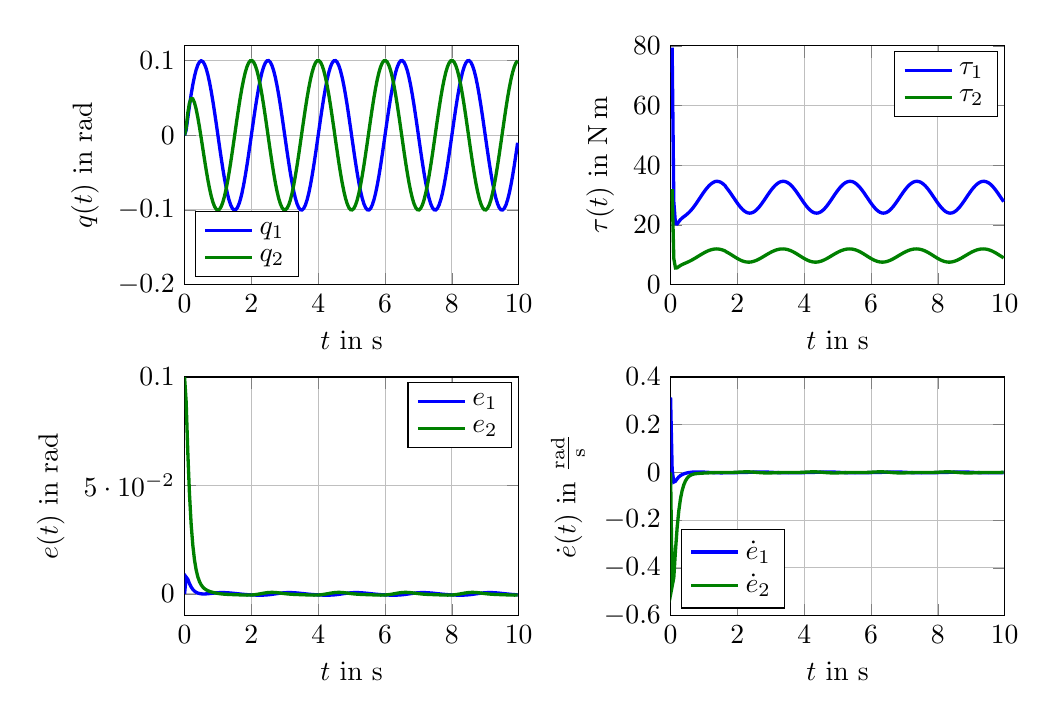
\begin{tikzpicture}

\begin{axis}[%
width=0.35\textwidth,
height=0.25\textwidth,
scale only axis,
xmin=0,
xmax=10,
xlabel={$t$ in $\mathrm{s}$},
xmajorgrids,
ymin=-0.2,
ymax=0.12,
ylabel={$q(t)$ in $\mathrm{rad}$},
ymajorgrids,
name=plot1,
legend style={at={(0.03,0.03)},anchor=south west,draw=black,fill=white,legend cell align=left}
]
\addplot [
color=blue,
solid,
line width=1.2pt
]
table[row sep=crcr]{
0 0\\
0.0476911628767132 0.00714583065705311\\
0.097 0.023227866953809\\
0.147 0.0397530980168608\\
0.197 0.0547900272274035\\
0.247 0.067945880576166\\
0.297 0.0790328045015822\\
0.347 0.0878934616618151\\
0.397 0.0943916733948735\\
0.447 0.0984241688488755\\
0.497 0.0999311453480991\\
0.547 0.0989033824851727\\
0.597 0.0953862809978635\\
0.647 0.0894812954572967\\
0.697 0.0813451095420508\\
0.747 0.0711868360649341\\
0.797 0.0592635032553539\\
0.847 0.0458740878937606\\
0.897 0.0313523586726289\\
0.947 0.0160587923385273\\
0.997 0.000371819038150653\\
1.04699999999999 -0.0153213568453261\\
1.09699999999999 -0.0306341258347542\\
1.14699999999998 -0.0451898092054146\\
1.19699999999998 -0.0586307478917073\\
1.24699999999997 -0.070626938877079\\
1.29699999999997 -0.0808840210702519\\
1.33225241581824 -0.0869323402203089\\
1.382 -0.0936420543430133\\
1.43199999999999 -0.098087950229716\\
1.48199999999999 -0.100121626255389\\
1.53199999999998 -0.0996934857614229\\
1.58199999999997 -0.0968143579984191\\
1.63199999999997 -0.0915551980316469\\
1.66725241581824 -0.0864823367390979\\
1.717 -0.0775432782093958\\
1.767 -0.066657318146689\\
1.817 -0.0541315749025856\\
1.867 -0.0402731678340139\\
1.917 -0.0254218774025556\\
1.967 -0.00994192353175101\\
2.017 0.00578683063513307\\
2.067 0.0213780563810549\\
2.117 0.036448319557251\\
2.167 0.050626418934135\\
2.217 0.0635624937346919\\
2.267 0.0749366880738357\\
2.317 0.0844671594267487\\
2.367 0.0919172216769611\\
2.417 0.0971014223621006\\
2.467 0.0998903702647045\\
2.517 0.100214155278744\\
2.567 0.0980642387222046\\
2.617 0.0934937388201949\\
2.667 0.0866160908417374\\
2.717 0.0776021201691815\\
2.767 0.0666756238577072\\
2.817 0.054107606361782\\
2.867 0.0402093537892389\\
2.917 0.0253245564059376\\
2.967 0.00982070187271117\\
3.017 -0.00592003542930575\\
3.067 -0.0215101870075166\\
3.117 -0.03656644903312\\
3.167 -0.0507189981413889\\
3.217 -0.0636204610891195\\
3.267 -0.0749543406354107\\
3.317 -0.0844427063016972\\
3.367 -0.0918529675012583\\
3.417 -0.0970035598902398\\
3.467 -0.0997683954536479\\
3.517 -0.100079953936832\\
3.567 -0.0979309278532502\\
3.617 -0.0933743741974509\\
3.667 -0.0865223705941873\\
3.717 -0.0775432184213227\\
3.767 -0.0666572767918843\\
3.817 -0.0541315462299739\\
3.867 -0.0402731479042168\\
3.917 -0.0254218635148311\\
3.967 -0.00994191383144295\\
4.01700000000001 0.00578683742472616\\
4.06700000000001 0.0213780611414243\\
4.11700000000001 0.0364483228991037\\
4.16700000000001 0.0506264212820766\\
4.21700000000001 0.0635624953849556\\
4.26700000000001 0.0749366892337349\\
4.31700000000001 0.0844671602417407\\
4.36700000000001 0.0919172222492995\\
4.41700000000001 0.097101422763756\\
4.46700000000001 0.0998903705463624\\
4.51700000000001 0.1002141554761\\
4.56700000000001 0.0980642388603858\\
4.61700000000001 0.0934937389168754\\
4.66700000000001 0.0866160909093374\\
4.71700000000001 0.0776021202164199\\
4.76700000000001 0.0666756238906985\\
4.81700000000001 0.0541076063848107\\
4.86700000000001 0.0402093538053049\\
4.91700000000001 0.0253245564171402\\
4.96700000000001 0.00982070188051815\\
5.01700000000001 -0.00592003542386817\\
5.06700000000001 -0.0215101870037315\\
5.11700000000001 -0.0365664490304864\\
5.16700000000001 -0.0507189981395572\\
5.21700000000001 -0.0636204610878459\\
5.26700000000001 -0.0749543406345255\\
5.31700000000001 -0.0844427063010822\\
5.36700000000001 -0.0918529675008313\\
5.41700000000001 -0.0970035598899437\\
5.46700000000001 -0.0997683954534434\\
5.51700000000001 -0.100079953936692\\
5.56700000000001 -0.0979309278531554\\
5.61700000000001 -0.0933743741973884\\
5.66700000000001 -0.0865223705941483\\
5.71700000000001 -0.0775432184213007\\
5.76700000000001 -0.0666572767918749\\
5.81700000000001 -0.0541315462299739\\
5.86700000000001 -0.0402731479042239\\
5.91700000000001 -0.0254218635148436\\
5.96700000000001 -0.00994191383145943\\
6.01700000000001 0.00578683742470692\\
6.06700000000001 0.0213780611414103\\
6.11700000000001 0.0364483228990936\\
6.16700000000001 0.0506264212820695\\
6.21700000000001 0.0635624953849506\\
6.26700000000001 0.0749366892337315\\
6.31700000000001 0.0844671602417384\\
6.36700000000001 0.0919172222492978\\
6.41700000000001 0.0971014227637548\\
6.46700000000001 0.0998903705463617\\
6.51700000000001 0.100214155476099\\
6.56700000000001 0.0980642388603854\\
6.61700000000001 0.0934937389168752\\
6.66700000000001 0.0866160909093373\\
6.71700000000001 0.0776021202164198\\
6.76700000000001 0.0666756238906984\\
6.81700000000001 0.0541076063848106\\
6.86700000000001 0.0402093538053048\\
6.91700000000001 0.0253245564171401\\
6.96700000000001 0.00982070188051805\\
7.01700000000001 -0.00592003542386821\\
7.06700000000001 -0.0215101870037314\\
7.11700000000001 -0.0365664490304863\\
7.16700000000001 -0.0507189981395572\\
7.21700000000001 -0.0636204610878459\\
7.26700000000001 -0.0749543406345255\\
7.31700000000001 -0.0844427063010822\\
7.36700000000001 -0.0918529675008313\\
7.41700000000001 -0.0970035598899438\\
7.46700000000001 -0.0997683954534434\\
7.51700000000001 -0.100079953936692\\
7.56700000000001 -0.0979309278531555\\
7.61700000000001 -0.0933743741973885\\
7.66700000000001 -0.0865223705941483\\
7.71700000000001 -0.0775432184213008\\
7.76700000000001 -0.066657276791875\\
7.81700000000001 -0.0541315462299739\\
7.86700000000001 -0.0402731479042239\\
7.91700000000001 -0.0254218635148437\\
7.96700000000001 -0.00994191383145946\\
8.01699999999999 0.00578683742470688\\
8.06699999999999 0.0213780611414236\\
8.11699999999999 0.0364483228991166\\
8.16699999999999 0.050626421282099\\
8.21699999999999 0.0635624953849833\\
8.26699999999999 0.0749366892337643\\
8.31699999999999 0.0844671602417695\\
8.36699999999999 0.0919172222493254\\
8.41699999999999 0.0971014227637779\\
8.46699999999999 0.099890370546379\\
8.51699999999999 0.10021415547611\\
8.56699999999999 0.0980642388603895\\
8.61699999999999 0.0934937389168723\\
8.66699999999999 0.0866160909093271\\
8.71699999999999 0.0776021202164024\\
8.76699999999999 0.0666756238906748\\
8.81699999999999 0.054107606384781\\
8.86699999999999 0.0402093538052701\\
8.91699999999999 0.0253245564171007\\
8.96699999999999 0.00982070188047489\\
9.01699999999999 -0.00592003542391354\\
9.06699999999999 -0.0215101870037781\\
9.11699999999999 -0.036566449030533\\
9.16699999999999 -0.050718998139603\\
9.21699999999999 -0.0636204610878899\\
9.26699999999999 -0.0749543406345661\\
9.31699999999999 -0.0844427063011186\\
9.36699999999999 -0.0918529675008625\\
9.41699999999999 -0.0970035598899693\\
9.46699999999999 -0.0997683954534625\\
9.51699999999999 -0.100079953936704\\
9.56699999999999 -0.0979309278531604\\
9.61699999999999 -0.093374374197386\\
9.66699999999999 -0.0865223705941387\\
9.71699999999999 -0.077543218421284\\
9.76699999999999 -0.0666572767918518\\
9.81699999999999 -0.0541315462299448\\
9.86699999999999 -0.0402731479041891\\
9.91699999999999 -0.0254218635148046\\
9.96699999999999 -0.00994191383141648\\
};
\addlegendentry{$q_1$};

\addplot [
color=green!50!black,
solid,
line width=1.2pt
]
table[row sep=crcr]{
0 0\\
0.0476911628767132 0.0102490190009673\\
0.097 0.0299894269207957\\
0.147 0.0433921497702168\\
0.197 0.0492446325873605\\
0.247 0.0489125332993333\\
0.297 0.0438198205084005\\
0.347 0.0351571086117227\\
0.397 0.0238986492759463\\
0.447 0.010856285194547\\
0.497 -0.00327585582973052\\
0.547 -0.0178908305350887\\
0.597 -0.0324499615554184\\
0.647 -0.0464722540767749\\
0.697 -0.059529429138905\\
0.747 -0.0712445394936812\\
0.797 -0.0812927093030709\\
0.847 -0.0894029747017018\\
0.897 -0.0953605140641526\\
0.947 -0.0990087699943942\\
0.997 -0.100251105723236\\
1.04699999999999 -0.0990517308022986\\
1.09699999999999 -0.0954356949008425\\
1.14699999999998 -0.0894877993448354\\
1.19699999999998 -0.0813503237290007\\
1.24699999999997 -0.0712195146783561\\
1.29699999999997 -0.0593408370458723\\
1.33225241581824 -0.0500705405925166\\
1.382 -0.0359716156117998\\
1.43199999999999 -0.0209148524542291\\
1.48199999999999 -0.00533707926040612\\
1.53199999999998 0.0103801558057471\\
1.58199999999997 0.0258512405061358\\
1.63199999999997 0.0406959144181421\\
1.66725241581824 0.0505902731872188\\
1.717 0.0634745913923783\\
1.767 0.0748725453743756\\
1.817 0.0844323106444437\\
1.867 0.0919153405901192\\
1.917 0.0971337512624571\\
1.967 0.0999552798245575\\
2.017 0.100306940007927\\
2.067 0.098177238896412\\
2.117 0.0936168449640107\\
2.167 0.0867376337157624\\
2.217 0.0777100838526936\\
2.267 0.0667590519559935\\
2.317 0.0541580149374186\\
2.367 0.0402219337882271\\
2.417 0.0252989550653605\\
2.467 0.00976122210698821\\
2.517 -0.00600489094240708\\
2.567 -0.0216087893971911\\
2.617 -0.0366655854159727\\
2.667 -0.0508056462759947\\
2.717 -0.063683517612896\\
2.767 -0.0749860351319471\\
2.817 -0.0844394950767295\\
2.867 -0.0918157981388473\\
2.917 -0.0969375085805376\\
2.967 -0.0996817809027336\\
3.017 -0.0999831058221375\\
3.067 -0.0978348232831093\\
3.117 -0.0932893501286435\\
3.167 -0.0864570792259299\\
3.217 -0.0775039277800588\\
3.267 -0.0666475450175718\\
3.317 -0.0541522309180776\\
3.367 -0.0403226641928619\\
3.417 -0.0254965842721066\\
3.467 -0.0100366133709062\\
3.517 0.00567856402869949\\
3.567 0.0212634289927686\\
3.617 0.0363350241588264\\
3.667 0.0505222871803783\\
3.717 0.0634751067428943\\
3.767 0.0748729043508137\\
3.817 0.084432560510509\\
3.867 0.0919155143741483\\
3.917 0.0971338720360125\\
3.967 0.0999553636944122\\
4.01700000000001 0.100306998209883\\
4.06700000000001 0.0981772792612432\\
4.11700000000001 0.0936168729439289\\
4.16700000000001 0.0867376531029916\\
4.21700000000001 0.0777100972822137\\
4.26700000000001 0.0667590612569665\\
4.31700000000001 0.0541580213785629\\
4.36700000000001 0.0402219382489201\\
4.41700000000001 0.0252989581547872\\
4.46700000000001 0.00976122424699381\\
4.51700000000001 -0.0060048894597761\\
4.56700000000001 -0.0216087883697713\\
4.61700000000001 -0.0366655847038217\\
4.66700000000001 -0.0508056457822329\\
4.71700000000001 -0.0636835172704473\\
4.76700000000001 -0.0749860348943621\\
4.81700000000001 -0.0844394949118367\\
4.86700000000001 -0.0918157980243598\\
4.91700000000001 -0.0969375085010126\\
4.96700000000001 -0.0996817808474685\\
5.01700000000001 -0.099983105783713\\
5.06700000000001 -0.0978348232563806\\
5.11700000000001 -0.0932893501100418\\
5.16700000000001 -0.0864570792129788\\
5.21700000000001 -0.077503927771039\\
5.26700000000001 -0.0666475450112891\\
5.31700000000001 -0.0541522309137018\\
5.36700000000001 -0.0403226641898155\\
5.41700000000001 -0.0254965842699879\\
5.46700000000001 -0.010036613369435\\
5.51700000000001 0.00567856402971875\\
5.56700000000001 0.0212634289934725\\
5.61700000000001 0.0363350241593104\\
5.66700000000001 0.0505222871807091\\
5.71700000000001 0.0634751067431189\\
5.76700000000001 0.074872904350965\\
5.81700000000001 0.0844325605106103\\
5.86700000000001 0.0919155143742156\\
5.91700000000001 0.0971338720360574\\
5.96700000000001 0.0999553636944426\\
6.01700000000001 0.100306998209905\\
6.06700000000001 0.0981772792612587\\
6.11700000000001 0.0936168729439397\\
6.16700000000001 0.0867376531029991\\
6.21700000000001 0.0777100972822189\\
6.26700000000001 0.0667590612569701\\
6.31700000000001 0.0541580213785652\\
6.36700000000001 0.0402219382489219\\
6.41700000000001 0.0252989581547885\\
6.46700000000001 0.00976122424699471\\
6.51700000000001 -0.00600488945977546\\
6.56700000000001 -0.0216087883697711\\
6.61700000000001 -0.0366655847038214\\
6.66700000000001 -0.0508056457822327\\
6.71700000000001 -0.0636835172704471\\
6.76700000000001 -0.074986034894362\\
6.81700000000001 -0.0844394949118366\\
6.86700000000001 -0.0918157980243597\\
6.91700000000001 -0.0969375085010125\\
6.96700000000001 -0.0996817808474684\\
7.01700000000001 -0.0999831057837129\\
7.06700000000001 -0.0978348232563806\\
7.11700000000001 -0.0932893501100418\\
7.16700000000001 -0.0864570792129788\\
7.21700000000001 -0.077503927771039\\
7.26700000000001 -0.0666475450112891\\
7.31700000000001 -0.0541522309137018\\
7.36700000000001 -0.0403226641898155\\
7.41700000000001 -0.0254965842699879\\
7.46700000000001 -0.0100366133694349\\
7.51700000000001 0.0056785640297188\\
7.56700000000001 0.0212634289934725\\
7.61700000000001 0.0363350241593104\\
7.66700000000001 0.0505222871807091\\
7.71700000000001 0.0634751067431189\\
7.76700000000001 0.074872904350965\\
7.81700000000001 0.0844325605106103\\
7.86700000000001 0.0919155143742156\\
7.91700000000001 0.0971338720360574\\
7.96700000000001 0.0999553636944425\\
8.01699999999999 0.100306998209905\\
8.06699999999999 0.0981772792612559\\
8.11699999999999 0.0936168729439322\\
8.16699999999999 0.0867376531029858\\
8.21699999999999 0.0777100972821993\\
8.26699999999999 0.0667590612569447\\
8.31699999999999 0.0541580213785342\\
8.36699999999999 0.0402219382488861\\
8.41699999999999 0.0252989581547483\\
8.46699999999999 0.00976122424695088\\
8.51699999999999 -0.0060048894598213\\
8.56699999999999 -0.0216087883698182\\
8.61699999999999 -0.0366655847038682\\
8.66699999999999 -0.0508056457822786\\
8.71699999999999 -0.063683517270491\\
8.76699999999999 -0.0749860348944024\\
8.81699999999999 -0.0844394949118729\\
8.86699999999999 -0.0918157980243908\\
8.91699999999999 -0.096937508501038\\
8.96699999999999 -0.0996817808474875\\
9.01699999999999 -0.0999831057837251\\
9.06699999999999 -0.0978348232563855\\
9.11699999999999 -0.0932893501100395\\
9.16699999999999 -0.0864570792129693\\
9.21699999999999 -0.0775039277710223\\
9.26699999999999 -0.066647545011266\\
9.31699999999999 -0.0541522309136726\\
9.36699999999999 -0.0403226641897813\\
9.41699999999999 -0.0254965842699489\\
9.46699999999999 -0.0100366133693922\\
9.51699999999999 0.00567856402976388\\
9.56699999999999 0.0212634289935191\\
9.61699999999999 0.0363350241593575\\
9.66699999999999 0.0505222871807551\\
9.71699999999999 0.0634751067431632\\
9.76699999999999 0.074872904351006\\
9.81699999999999 0.0844325605106472\\
9.86699999999999 0.0919155143742476\\
9.91699999999999 0.0971338720360834\\
9.96699999999999 0.0999553636944621\\
};
\addlegendentry{$q_2$};

\end{axis}

\begin{axis}[%
width=0.35\textwidth,
height=0.25\textwidth,
scale only axis,
xmin=0,
xmax=10,
xlabel={$t$ in $\mathrm{s}$},
xmajorgrids,
ymin=-0.01,
ymax=0.1,
ylabel={$e(t)$ in $\mathrm{rad}$},
ymajorgrids,
name=plot3,
at=(plot1.below south west),
anchor=above north west,
legend style={draw=black,fill=white,legend cell align=left}
]
\addplot [
color=blue,
solid,
line width=1.2pt
]
table[row sep=crcr]{
0 0\\
0.0476911628767132 0.00778079820905389\\
0.097 0.00677612367031867\\
0.147 0.00480419422082884\\
0.197 0.00322341821178142\\
0.247 0.00209523450221466\\
0.297 0.00131133550963061\\
0.347 0.000775363908240539\\
0.397 0.000418516973529681\\
0.447 0.000192844774023412\\
0.497 6.44133627958621e-05\\
0.547 8.4987920234425e-06\\
0.597 6.38405887584681e-06\\
0.647 4.32693751844099e-05\\
0.697 0.00010696316500014\\
0.747 0.000187124162708011\\
0.797 0.000274880715481547\\
0.847 0.000362687210338615\\
0.897 0.000444304710612194\\
0.947 0.000514819944284695\\
0.997 0.000570644805163746\\
1.04699999999999 0.000609465661464022\\
1.09699999999999 0.000630135210629768\\
1.14699999999998 0.000632516967729549\\
1.19699999999998 0.000617302452527911\\
1.24699999999997 0.000585823798704491\\
1.29699999999997 0.000539881059045219\\
1.33225241581824 0.000500088968797177\\
1.382 0.000434943097192636\\
1.43199999999999 0.00036113787289728\\
1.48199999999999 0.000281471244492196\\
1.53199999999998 0.00019838406329227\\
1.58199999999997 0.000114209222173547\\
1.63199999999997 3.10807695511894e-05\\
1.66725241581824 -2.8047799446082e-05\\
1.717 -0.00010537305931238\\
1.767 -0.000177883870090809\\
1.817 -0.000244473375294173\\
1.867 -0.000304807932606677\\
1.917 -0.000358861418850859\\
1.967 -0.000406770993291774\\
2.017 -0.000448661659257649\\
2.067 -0.000484467340814213\\
2.117 -0.000513779956662512\\
2.167 -0.000535756398064594\\
2.217 -0.00054910661615544\\
2.267 -0.000552175093133656\\
2.317 -0.000543114161510844\\
2.367 -0.000520132649555277\\
2.417 -0.000481789233929303\\
2.467 -0.000427289065561332\\
2.517 -0.000356737166792839\\
2.567 -0.000271304739132339\\
2.617 -0.000173275556804811\\
2.667 -6.59578164352581e-05\\
2.717 4.65310995267226e-05\\
2.767 0.000159578159072568\\
2.817 0.000268441916097692\\
2.867 0.000368621977381696\\
2.917 0.000456182415468895\\
2.967 0.000527992652331711\\
3.017 0.000581866453430249\\
3.067 0.00061659796727586\\
3.117 0.000631909432531427\\
3.167 0.000628335605318345\\
3.217 0.000607073970582989\\
3.267 0.00056982765470863\\
3.317 0.000518661036459339\\
3.367 0.000455878473852478\\
3.417 0.000383926762068484\\
3.467 0.000305314254504682\\
3.517 0.000222535824881451\\
3.567 0.00013799387017796\\
3.617 5.3910934060819e-05\\
3.667 -2.77624311148389e-05\\
3.717 -0.000105432847385512\\
3.767 -0.0001779252248955\\
3.817 -0.000244502047905784\\
3.867 -0.000304827862403746\\
3.917 -0.00035887530657543\\
3.967 -0.000406780693599947\\
4.01700000000001 -0.000448668448848369\\
4.06700000000001 -0.000484472101181549\\
4.11700000000001 -0.000513783298512843\\
4.16700000000001 -0.000535758746003992\\
4.21700000000001 -0.000549108266417284\\
4.26700000000001 -0.000552176253031333\\
4.31700000000001 -0.000543114976501557\\
4.36700000000001 -0.000520133221892607\\
4.41700000000001 -0.000481789635584012\\
4.46700000000001 -0.000427289347219015\\
4.51700000000001 -0.000356737364148915\\
4.56700000000001 -0.000271304877313999\\
4.61700000000001 -0.000173275653486252\\
4.66700000000001 -6.59578840364605e-05\\
4.71700000000001 4.65310522868995e-05\\
4.76700000000001 0.000159578126079543\\
4.81700000000001 0.000268441893066955\\
4.86700000000001 0.000368621961313452\\
4.91700000000001 0.000456182404263948\\
4.96700000000001 0.000527992644522286\\
5.01700000000001 0.000581866447990386\\
5.06700000000001 0.000616597963488338\\
5.11700000000001 0.000631909429895682\\
5.16700000000001 0.000628335603484603\\
5.21700000000001 0.000607073969307495\\
5.26700000000001 0.000569827653821908\\
5.31700000000001 0.00051866103584286\\
5.36700000000001 0.000455878473424459\\
5.41700000000001 0.000383926761771777\\
5.46700000000001 0.000305314254299971\\
5.51700000000001 0.000222535824741313\\
5.56700000000001 0.000137993870083633\\
5.61700000000001 5.39109339992572e-05\\
5.66700000000001 -2.77624311526142e-05\\
5.71700000000001 -0.000105432847406037\\
5.76700000000001 -0.00017792522490305\\
5.81700000000001 -0.000244502047903786\\
5.86700000000001 -0.000304827862394268\\
5.91700000000001 -0.000358875306560674\\
5.96700000000001 -0.000406780693581018\\
6.01700000000001 -0.000448668448829328\\
6.06700000000001 -0.000484472101167161\\
6.11700000000001 -0.000513783298502893\\
6.16700000000001 -0.000535758745996921\\
6.21700000000001 -0.00054910826641219\\
6.26700000000001 -0.000552176253027864\\
6.31700000000001 -0.000543114976499115\\
6.36700000000001 -0.000520133221890984\\
6.41700000000001 -0.00048178963558286\\
6.46700000000001 -0.000427289347218252\\
6.51700000000001 -0.000356737364148485\\
6.56700000000001 -0.000271304877313638\\
6.61700000000001 -0.000173275653485988\\
6.66700000000001 -6.59578840364189e-05\\
6.71700000000001 4.65310522869966e-05\\
6.76700000000001 0.000159578126079515\\
6.81700000000001 0.000268441893067045\\
6.86700000000001 0.000368621961313417\\
6.91700000000001 0.000456182404264247\\
6.96700000000001 0.000527992644522407\\
7.01700000000001 0.000581866447990624\\
7.06700000000001 0.000616597963488341\\
7.11700000000001 0.000631909429895682\\
7.16700000000001 0.00062833560348461\\
7.21700000000001 0.000607073969307509\\
7.26700000000001 0.000569827653821922\\
7.31700000000001 0.000518661035842874\\
7.36700000000001 0.000455878473424473\\
7.41700000000001 0.000383926761771805\\
7.46700000000001 0.000305314254299985\\
7.51700000000001 0.000222535824741327\\
7.56700000000001 0.000137993870083675\\
7.61700000000001 5.39109339992988e-05\\
7.66700000000001 -2.77624311525865e-05\\
7.71700000000001 -0.000105432847406037\\
7.76700000000001 -0.000177925224903022\\
7.81700000000001 -0.000244502047903744\\
7.86700000000001 -0.000304827862394247\\
7.91700000000001 -0.000358875306560653\\
7.96700000000001 -0.000406780693581014\\
8.01699999999999 -0.000448668448833921\\
8.06699999999999 -0.00048447210118532\\
8.11699999999999 -0.000513783298530614\\
8.16699999999999 -0.00053575874603045\\
8.21699999999999 -0.000549108266448509\\
8.26699999999999 -0.000552176253063849\\
8.31699999999999 -0.000543114976532949\\
8.36699999999999 -0.000520133221920599\\
8.41699999999999 -0.000481789635607216\\
8.46699999999999 -0.000427289347236084\\
8.51699999999999 -0.000356737364159115\\
8.56699999999999 -0.000271304877316747\\
8.61699999999999 -0.000173275653481283\\
8.66699999999999 -6.59578840236513e-05\\
8.71699999999999 4.65310523071055e-05\\
8.76699999999999 0.000159578126106882\\
8.81699999999999 0.000268441893100581\\
8.86699999999999 0.000368621961352657\\
8.91699999999999 0.000456182404308125\\
8.96699999999999 0.00052799264457019\\
9.01699999999999 0.000581866448040595\\
9.06699999999999 0.000616597963539928\\
9.11699999999999 0.000631909429946953\\
9.16699999999999 0.000628335603534501\\
9.21699999999999 0.000607073969355124\\
9.26699999999999 0.000569827653865637\\
9.31699999999999 0.000518661035881995\\
9.36699999999999 0.000455878473457724\\
9.41699999999999 0.000383926761798631\\
9.46699999999999 0.000305314254319497\\
9.51699999999999 0.000222535824753262\\
9.56699999999999 0.00013799387008763\\
9.61699999999999 5.39109339951632e-05\\
9.66699999999999 -2.77624311647018e-05\\
9.71699999999999 -0.000105432847425466\\
9.76699999999999 -0.000177925224929876\\
9.81699999999999 -0.000244502047936801\\
9.86699999999999 -0.000304827862433313\\
9.91699999999999 -0.000358875306604257\\
9.96699999999999 -0.000406780693628607\\
};
\addlegendentry{$e_1$};

\addplot [
color=green!50!black,
solid,
line width=1.2pt
]
table[row sep=crcr]{
0 0.1\\
0.0476911628767132 0.0886306844304929\\
0.097 0.0654032381359437\\
0.147 0.0461324150622644\\
0.197 0.0322074401196904\\
0.247 0.0224614269283089\\
0.297 0.0157185634624349\\
0.347 0.0110796664923765\\
0.397 0.00789801410729476\\
0.447 0.00571732708826492\\
0.497 0.00421831967304491\\
0.547 0.00317893935122495\\
0.597 0.00244597093129078\\
0.647 0.0019149618390852\\
0.697 0.00151598369972004\\
0.747 0.00120342441530052\\
0.797 0.000948569291858187\\
0.847 0.000734149131646156\\
0.897 0.00055032369574938\\
0.947 0.000391756371495328\\
0.997 0.000255547012341054\\
1.04699999999999 0.000139849525102126\\
1.09699999999999 4.3029844102177e-05\\
1.14699999999998 -3.6765487648055e-05\\
1.19699999999998 -0.000101748978054206\\
1.24699999999997 -0.000154445549292045\\
1.29699999999997 -0.000197546924971405\\
1.33225241581824 -0.000223255680935903\\
1.382 -0.000255921058655753\\
1.43199999999999 -0.000285858537979179\\
1.48199999999999 -0.000314774187800878\\
1.53199999999998 -0.000343984320631867\\
1.58199999999997 -0.000374167937805332\\
1.63199999999997 -0.000405270846784767\\
1.66725241581824 -0.000430993218371124\\
1.717 -0.000461204273841789\\
1.767 -0.000488032393673496\\
1.817 -0.000508265379205897\\
1.867 -0.000518251562713304\\
1.917 -0.000514118134285743\\
1.967 -0.000492198625414345\\
2.017 -0.00044952189597626\\
2.067 -0.000384304913339698\\
2.117 -0.000296381700620657\\
2.167 -0.000187500690460238\\
2.217 -6.14325839854019e-05\\
2.267 7.61500607862758e-05\\
2.317 0.000218033340461117\\
2.367 0.0003560419783935\\
2.417 0.000481783756046014\\
2.467 0.000587472418054576\\
2.517 0.000666721966531663\\
2.567 0.000715200356950413\\
2.617 0.000731045815384135\\
2.667 0.000714983739924069\\
2.717 0.000670130494359503\\
2.767 0.00060152215124501\\
2.817 0.000515449811491597\\
2.867 0.000418709111441443\\
2.917 0.000317875452366306\\
2.967 0.000218699703590411\\
3.017 0.000125687710186478\\
3.067 4.18893000370402e-05\\
3.117 -3.11131347465604e-05\\
3.167 -9.30537993722586e-05\\
3.217 -0.000144723488649426\\
3.267 -0.000187656999207975\\
3.317 -0.00022381735980212\\
3.367 -0.000255311573758729\\
3.417 -0.000284154549299941\\
3.467 -0.000312081154136661\\
3.517 -0.000340395052823999\\
3.567 -0.000369839952527869\\
3.617 -0.000400484558237803\\
3.667 -0.000431624644307675\\
3.717 -0.000461719624357801\\
3.767 -0.000488391370111627\\
3.817 -0.000508515245271179\\
3.867 -0.000518425346742402\\
3.917 -0.000514238907841219\\
3.967 -0.000492282495269017\\
4.01700000000001 -0.000449580097932376\\
4.06700000000001 -0.000384345278171397\\
4.11700000000001 -0.000296409680539719\\
4.16700000000001 -0.000187520077690642\\
4.21700000000001 -6.14460135069245e-05\\
4.26700000000001 7.61407598116048e-05\\
4.31700000000001 0.00021802689931489\\
4.36700000000001 0.000356037517698249\\
4.41700000000001 0.000481780666616884\\
4.46700000000001 0.00058747027804662\\
4.51700000000001 0.000666720483898309\\
4.56700000000001 0.000715199329528522\\
4.61700000000001 0.000731045103230868\\
4.66700000000001 0.000714983246160351\\
4.71700000000001 0.000670130151909018\\
4.76700000000001 0.00060152191365849\\
4.81700000000001 0.000515449646597527\\
4.86700000000001 0.000418708996952885\\
4.91700000000001 0.000317875372840615\\
4.96700000000001 0.000218699648325091\\
5.01700000000001 0.000125687671762104\\
5.06700000000001 4.18892733088649e-05\\
5.11700000000001 -3.11131533474729e-05\\
5.16700000000001 -9.30538123221636e-05\\
5.21700000000001 -0.00014472349766767\\
5.26700000000001 -0.000187657005489034\\
5.31700000000001 -0.000223817364175732\\
5.36700000000001 -0.000255311576802843\\
5.41700000000001 -0.000284154551416241\\
5.46700000000001 -0.000312081155605616\\
5.51700000000001 -0.000340395053840971\\
5.56700000000001 -0.000369839953229551\\
5.61700000000001 -0.000400484558719508\\
5.66700000000001 -0.000431624644636343\\
5.71700000000001 -0.000461719624580623\\
5.76700000000001 -0.000488391370261285\\
5.81700000000001 -0.000508515245371113\\
5.86700000000001 -0.000518425346808668\\
5.91700000000001 -0.000514238907885434\\
5.96700000000001 -0.000492282495299132\\
6.01700000000001 -0.000449580097954025\\
6.06700000000001 -0.000384345278186912\\
6.11700000000001 -0.000296409680550447\\
6.16700000000001 -0.000187520077698122\\
6.21700000000001 -6.14460135122535e-05\\
6.26700000000001 7.61407598080105e-05\\
6.31700000000001 0.000218026899312329\\
6.36700000000001 0.000356037517696473\\
6.41700000000001 0.000481780666615649\\
6.46700000000001 0.000587470278045924\\
6.51700000000001 0.000666720483897698\\
6.56700000000001 0.00071519932952821\\
6.61700000000001 0.00073104510323059\\
6.66700000000001 0.00071498324615997\\
6.71700000000001 0.000670130151908893\\
6.76700000000001 0.000601521913658268\\
6.81700000000001 0.00051544964659743\\
6.86700000000001 0.000418708996952746\\
6.91700000000001 0.000317875372840615\\
6.96700000000001 0.000218699648325021\\
7.01700000000001 0.000125687671762034\\
7.06700000000001 4.18892733088094e-05\\
7.11700000000001 -3.11131533474868e-05\\
7.16700000000001 -9.30538123221775e-05\\
7.21700000000001 -0.000144723497667656\\
7.26700000000001 -0.00018765700548902\\
7.31700000000001 -0.00022381736417576\\
7.36700000000001 -0.000255311576802864\\
7.41700000000001 -0.000284154551416307\\
7.46700000000001 -0.000312081155605694\\
7.51700000000001 -0.000340395053841043\\
7.56700000000001 -0.000369839953229621\\
7.61700000000001 -0.00040048455871957\\
7.66700000000001 -0.000431624644636384\\
7.71700000000001 -0.00046171962458065\\
7.76700000000001 -0.000488391370261326\\
7.81700000000001 -0.000508515245371141\\
7.86700000000001 -0.000518425346808668\\
7.91700000000001 -0.000514238907885448\\
7.96700000000001 -0.00049228249529909\\
8.01699999999999 -0.000449580097953761\\
8.06699999999999 -0.000384345278183054\\
8.11699999999999 -0.000296409680541149\\
8.16699999999999 -0.000187520077682468\\
8.21699999999999 -6.1446013489716e-05\\
8.26699999999999 7.61407598368347e-05\\
8.31699999999999 0.000218026899347488\\
8.36699999999999 0.000356037517736767\\
8.41699999999999 0.000481780666660721\\
8.46699999999999 0.000587470278094018\\
8.51699999999999 0.000666720483948174\\
8.56699999999999 0.000715199329579759\\
8.61699999999999 0.000731045103282021\\
8.66699999999999 0.000714983246210187\\
8.71699999999999 0.000670130151956105\\
8.76699999999999 0.000601521913702066\\
8.81699999999999 0.00051544964663619\\
8.86699999999999 0.000418708996985914\\
8.91699999999999 0.000317875372867288\\
8.96699999999999 0.000218699648344534\\
9.01699999999999 0.000125687671773941\\
9.06699999999999 4.18892733126952e-05\\
9.11699999999999 -3.11131533515391e-05\\
9.16699999999999 -9.3053812334043e-05\\
9.21699999999999 -0.000144723497687307\\
9.26699999999999 -0.000187657005515582\\
9.31699999999999 -0.000223817364209067\\
9.36699999999999 -0.00025531157684161\\
9.41699999999999 -0.00028415455146007\\
9.46699999999999 -0.000312081155652731\\
9.51699999999999 -0.000340395053890767\\
9.56699999999999 -0.000369839953280729\\
9.61699999999999 -0.000400484558770994\\
9.66699999999999 -0.000431624644686719\\
9.71699999999999 -0.000461719624628251\\
9.76699999999999 -0.000488391370305652\\
9.81699999999999 -0.00050851524541054\\
9.86699999999999 -0.000518425346842585\\
9.91699999999999 -0.000514238907912731\\
9.96699999999999 -0.000492282495319199\\
};
\addlegendentry{$e_2$};

\end{axis}

\begin{axis}[%
width=0.35\textwidth,
height=0.25\textwidth,
scale only axis,
xmin=0,
xmax=10,
xlabel={$t$ in $\mathrm{s}$},
xmajorgrids,
ymin=-0.6,
ymax=0.4,
ylabel={$\dot{e}(t)$ in $\mathrm{\frac{rad}{s}}$},
ymajorgrids,
name=plot2,
at=(plot3.right of south east),
anchor=left of south west,
legend style={at={(0.03,0.03)},anchor=south west,draw=black,fill=white,legend cell align=left}
]
\addplot [
color=blue,
solid,
line width=1.2pt
]
table[row sep=crcr]{
0 0.314159265358979\\
0.0476911628767132 0.0109314018732356\\
0.097 -0.0402794818504185\\
0.147 -0.0367359068320442\\
0.197 -0.0269398529470627\\
0.247 -0.0189425957002773\\
0.297 -0.0131237534090214\\
0.347 -0.00891552970119031\\
0.397 -0.00582606459778943\\
0.447 -0.00351864970153493\\
0.497 -0.0017725232025617\\
0.547 -0.000445129878735989\\
0.597 0.000554545856789865\\
0.647 0.00128468361530454\\
0.697 0.00178398123257553\\
0.747 0.00208106406833228\\
0.797 0.00220071464323529\\
0.847 0.00216746745553792\\
0.897 0.00200709877105981\\
0.947 0.00174658644283693\\
0.997 0.00141313546489813\\
1.04699999999999 0.00103282347882067\\
1.09699999999999 0.000629314778537116\\
1.14699999999998 0.000222941545626298\\
1.19699999999998 -0.000169713692642293\\
1.24699999999997 -0.000535751418283797\\
1.29699999999997 -0.000865535995720146\\
1.33225241581824 -0.00131697342524634\\
1.382 -0.00147246000652845\\
1.43199999999999 -0.00157819454441485\\
1.48199999999999 -0.00163554187461971\\
1.53199999999998 -0.0016466121233675\\
1.58199999999997 -0.00161511143859895\\
1.63199999999997 -0.00154641768737881\\
1.66725241581824 -0.00147204020338673\\
1.717 -0.00136430889968062\\
1.767 -0.00123660073424692\\
1.817 -0.00110050840290021\\
1.867 -0.000963058299864761\\
1.917 -0.000829025169040987\\
1.967 -0.00070015649512517\\
2.017 -0.000574838739894223\\
2.067 -0.000448321062428814\\
2.117 -0.000313516803698344\\
2.167 -0.000162303806037267\\
2.217 1.28428803511105e-05\\
2.267 0.000217117902807457\\
2.317 0.000451821085420356\\
2.367 0.000713233099272903\\
2.417 0.000992165197639894\\
2.467 0.00127433436678692\\
2.517 0.00154159051839544\\
2.567 0.00177387060824546\\
2.617 0.00195160529334733\\
2.667 0.00205819511143884\\
2.717 0.00208213956995257\\
2.767 0.0020184603072832\\
2.817 0.00186919822574477\\
2.867 0.00164294897943051\\
2.917 0.00135358353471837\\
2.967 0.00101843660074741\\
3.017 0.000656308587190568\\
3.067 0.000285611875876501\\
3.117 -7.70855250842861e-05\\
3.167 -0.000417980290537689\\
3.217 -0.000726401924445758\\
3.267 -0.000994718664089844\\
3.317 -0.00121794313007825\\
3.367 -0.00139322807617365\\
3.417 -0.00151942518948879\\
3.467 -0.00159682243383011\\
3.517 -0.00162709167312379\\
3.567 -0.00161338914617029\\
3.617 -0.00156048126960431\\
3.667 -0.00147473886222607\\
3.717 -0.00136386548426615\\
3.767 -0.00123629584718285\\
3.817 -0.00110029840650983\\
3.867 -0.000962913335000426\\
3.917 -0.000828924829941291\\
3.967 -0.000700086842182701\\
4.01700000000001 -0.000574790245393808\\
4.06700000000001 -0.000448287203964171\\
4.11700000000001 -0.000313493104850737\\
4.16700000000001 -0.000162287184180099\\
4.21700000000001 1.28545564244409e-05\\
4.26700000000001 0.000217126112762561\\
4.31700000000001 0.000451826860846993\\
4.36700000000001 0.000713237162091679\\
4.41700000000001 0.00099216805464529\\
4.46700000000001 0.00127433637458651\\
4.51700000000001 0.00154159192828561\\
4.56700000000001 0.00177387159742937\\
4.61700000000001 0.00195160598677122\\
4.66700000000001 0.00205819559714962\\
4.71700000000001 0.00208213990993358\\
4.76700000000001 0.0020184605451177\\
4.81700000000001 0.00186919839204092\\
4.86700000000001 0.00164294909565832\\
4.91700000000001 0.00135358361592364\\
4.96700000000001 0.00101843665746665\\
5.01700000000001 0.000656308626795665\\
5.06700000000001 0.000285611903523941\\
5.11700000000001 -7.70855057895536e-05\\
5.16700000000001 -0.000417980277074459\\
5.21700000000001 -0.000726401915052105\\
5.26700000000001 -0.000994718657537669\\
5.31700000000001 -0.0012179431255068\\
5.36700000000001 -0.00139322807298453\\
5.41700000000001 -0.00151942518726456\\
5.46700000000001 -0.00159682243228117\\
5.51700000000001 -0.00162709167204835\\
5.56700000000001 -0.00161338914542866\\
5.61700000000001 -0.00156048126909872\\
5.66700000000001 -0.00147473886188934\\
5.71700000000001 -0.0013638654840544\\
5.76700000000001 -0.00123629584706214\\
5.81700000000001 -0.00110029840645703\\
5.86700000000001 -0.000962913334999316\\
5.91700000000001 -0.000828924829979427\\
5.96700000000001 -0.000700086842251868\\
6.01700000000001 -0.000574790245485568\\
6.06700000000001 -0.000448287204059539\\
6.11700000000001 -0.000313493104922569\\
6.16700000000001 -0.000162287184231502\\
6.21700000000001 1.28545563878313e-05\\
6.26700000000001 0.000217126112737526\\
6.31700000000001 0.000451826860829202\\
6.36700000000001 0.000713237162079938\\
6.41700000000001 0.000992168054637158\\
6.46700000000001 0.00127433637458075\\
6.51700000000001 0.00154159192828199\\
6.56700000000001 0.00177387159742808\\
6.61700000000001 0.00195160598676961\\
6.66700000000001 0.00205819559714754\\
6.71700000000001 0.00208213990993306\\
6.76700000000001 0.00201846054511751\\
6.81700000000001 0.00186919839204086\\
6.86700000000001 0.00164294909565849\\
6.91700000000001 0.00135358361592364\\
6.96700000000001 0.00101843665746609\\
7.01700000000001 0.000656308626794277\\
7.06700000000001 0.000285611903523109\\
7.11700000000001 -7.70855057897757e-05\\
7.16700000000001 -0.000417980277074237\\
7.21700000000001 -0.000726401915052077\\
7.26700000000001 -0.00099471865753728\\
7.31700000000001 -0.0012179431255066\\
7.36700000000001 -0.00139322807298445\\
7.41700000000001 -0.00151942518726426\\
7.46700000000001 -0.00159682243228122\\
7.51700000000001 -0.0016270916720482\\
7.56700000000001 -0.00161338914542856\\
7.61700000000001 -0.00156048126909902\\
7.66700000000001 -0.00147473886188992\\
7.71700000000001 -0.00136386548405465\\
7.76700000000001 -0.00123629584706211\\
7.81700000000001 -0.00110029840645731\\
7.86700000000001 -0.000962913334999538\\
7.91700000000001 -0.000828924829979649\\
7.96700000000001 -0.000700086842251868\\
8.01699999999999 -0.000574790245484513\\
8.06699999999999 -0.000448287204030895\\
8.11699999999999 -0.000313493104823592\\
8.16699999999999 -0.000162287184077403\\
8.21699999999999 1.28545565780402e-05\\
8.26699999999999 0.000217126112945693\\
8.31699999999999 0.000451826861042254\\
8.36699999999999 0.000713237162284663\\
8.41699999999999 0.000992168054825479\\
8.46699999999999 0.00127433637474352\\
8.51699999999999 0.00154159192841396\\
8.56699999999999 0.00177387159752412\\
8.61699999999999 0.00195160598682713\\
8.66699999999999 0.00205819559716522\\
8.71699999999999 0.00208213990990544\\
8.76699999999999 0.00201846054504812\\
8.81699999999999 0.00186919839193156\\
8.86699999999999 0.00164294909551149\\
8.91699999999999 0.00135358361574195\\
8.96699999999999 0.00101843665725471\\
9.01699999999999 0.000656308626558466\\
9.06699999999999 0.000285611903268035\\
9.11699999999999 -7.70855060581721e-05\\
9.16699999999999 -0.000417980277348684\\
9.21699999999999 -0.000726401915326136\\
9.26699999999999 -0.000994718657803734\\
9.31699999999999 -0.00121794312576018\\
9.36699999999999 -0.00139322807321676\\
9.41699999999999 -0.00151942518747175\\
9.46699999999999 -0.00159682243245638\\
9.51699999999999 -0.0016270916721879\\
9.56699999999999 -0.0016133891455298\\
9.61699999999999 -0.00156048126916032\\
9.66699999999999 -0.00147473886190869\\
9.71699999999999 -0.00136386548402911\\
9.76699999999999 -0.00123629584699494\\
9.81699999999999 -0.00110029840635012\\
9.86699999999999 -0.00096291333485532\\
9.91699999999999 -0.000828924829800515\\
9.96699999999999 -0.000700086842042591\\
};
\addlegendentry{$\dot{e}_1$};

\addplot [
color=green!50!black,
solid,
line width=1.2pt
]
table[row sep=crcr]{
0 -0\\
0.0476911628767132 -0.476632382897735\\
0.097 -0.440569473462962\\
0.147 -0.327196471760818\\
0.197 -0.230774852958785\\
0.247 -0.160038669152871\\
0.297 -0.110106605639596\\
0.347 -0.0753797313532858\\
0.397 -0.0514496858319103\\
0.447 -0.0351062173653255\\
0.497 -0.0240616061446365\\
0.547 -0.0166932904729223\\
0.597 -0.0118494321267453\\
0.647 -0.00871118456535724\\
0.697 -0.00669755939526032\\
0.747 -0.00540007119693942\\
0.797 -0.00453725912312866\\
0.847 -0.00392202528800212\\
0.897 -0.00343710708459395\\
0.947 -0.00301583315804117\\
0.997 -0.00262660918569683\\
1.04699999999999 -0.00226039613422385\\
1.09699999999999 -0.00192087132960757\\
1.14699999999998 -0.00161711005719173\\
1.19699999999998 -0.00135859915396649\\
1.24699999999997 -0.00115228494871278\\
1.29699999999997 -0.00100123580330874\\
1.33225241581824 -0.000576806940619679\\
1.382 -0.000486367667898391\\
1.43199999999999 -0.000438558549349266\\
1.48199999999999 -0.00042129270197161\\
1.53199999999998 -0.000423153407446086\\
1.58199999999997 -0.000431093220093492\\
1.63199999999997 -0.00043063729826609\\
1.66725241581824 -0.000424943311737702\\
1.717 -0.000384079081945682\\
1.767 -0.000289743470233361\\
1.817 -0.000135449321227332\\
1.867 8.56319993876309e-05\\
1.917 0.000373392247356538\\
1.967 0.000719286300289938\\
2.017 0.00110574027127308\\
2.067 0.00150672929991164\\
2.117 0.00188961604726419\\
2.167 0.00221815469951961\\
2.217 0.00245638703654252\\
2.267 0.0025730012621448\\
2.317 0.0025456027582868\\
2.367 0.00236427659603267\\
2.417 0.00203383139629171\\
2.467 0.00157423168880239\\
2.517 0.00101896502274285\\
2.567 0.000411430713636529\\
2.617 -0.000200183471397497\\
2.667 -0.000768746906824991\\
2.717 -0.00125379277358567\\
2.767 -0.00162596454764577\\
2.817 -0.00186962822269454\\
2.867 -0.00198336217948922\\
2.917 -0.00197845498118396\\
2.967 -0.00187588678058707\\
3.017 -0.00170247193496545\\
3.067 -0.00148687791456785\\
3.117 -0.0012561317277642\\
3.167 -0.00103302879913872\\
3.217 -0.00083462569081505\\
3.267 -0.000671775323290963\\
3.317 -0.000549487337940524\\
3.367 -0.000467790961736159\\
3.417 -0.000422756223843801\\
3.467 -0.000407392099114168\\
3.517 -0.000412271266462427\\
3.567 -0.000425896421132721\\
3.617 -0.0004349741440412\\
3.667 -0.00042484954852412\\
3.717 -0.000380345048433123\\
3.767 -0.000287137472338772\\
3.817 -0.000133631651538818\\
3.867 8.68989024576661e-05\\
3.917 0.000374274548597273\\
3.967 0.000719900218445937\\
4.01700000000001 0.00110616706454613\\
4.06700000000001 0.00150702574859307\\
4.11700000000001 0.00188982179445508\\
4.16700000000001 0.00221829739542478\\
4.21700000000001 0.00245648594481429\\
4.26700000000001 0.00257306978775973\\
4.31700000000001 0.00254565021847847\\
4.36700000000001 0.00236430945975613\\
4.41700000000001 0.00203385415060847\\
4.46700000000001 0.00157424744357609\\
4.51700000000001 0.00101897593199857\\
4.56700000000001 0.000411438268692887\\
4.61700000000001 -0.000200178238307258\\
4.66700000000001 -0.000768743281309603\\
4.71700000000001 -0.00125379026122283\\
4.76700000000001 -0.00162596280621757\\
4.81700000000001 -0.00186962701530133\\
4.86700000000001 -0.00198336134210655\\
4.91700000000001 -0.00197845440022489\\
4.96700000000001 -0.00187588637737892\\
5.01700000000001 -0.00170247165500886\\
5.06700000000001 -0.0014868777201012\\
5.11700000000001 -0.0012561315926178\\
5.16700000000001 -0.00103302870517238\\
5.21700000000001 -0.000834625625451751\\
5.26700000000001 -0.000671775277805459\\
5.31700000000001 -0.000549487306280905\\
5.36700000000001 -0.000467790939701229\\
5.41700000000001 -0.000422756208511121\\
5.46700000000001 -0.000407392088455139\\
5.51700000000001 -0.000412271259064345\\
5.56700000000001 -0.000425896416010818\\
5.61700000000001 -0.000434974140509636\\
5.66700000000001 -0.000424849546101447\\
5.71700000000001 -0.000380345046782415\\
5.76700000000001 -0.000287137471224996\\
5.81700000000001 -0.000133631650795468\\
5.86700000000001 8.68989029472189e-05\\
5.91700000000001 0.00037427454891574\\
5.96700000000001 0.000719900218650232\\
6.01700000000001 0.00110616706468665\\
6.06700000000001 0.00150702574870147\\
6.11700000000001 0.00188982179453348\\
6.16700000000001 0.00221829739547957\\
6.21700000000001 0.00245648594485232\\
6.26700000000001 0.00257306978778615\\
6.31700000000001 0.00254565021849623\\
6.36700000000001 0.00236430945976801\\
6.41700000000001 0.00203385415061746\\
6.46700000000001 0.00157424744358253\\
6.51700000000001 0.00101897593200312\\
6.56700000000001 0.000411438268696329\\
6.61700000000001 -0.000200178238305204\\
6.66700000000001 -0.000768743281308104\\
6.71700000000001 -0.00125379026122135\\
6.76700000000001 -0.00162596280621655\\
6.81700000000001 -0.00186962701530105\\
6.86700000000001 -0.00198336134210558\\
6.91700000000001 -0.0019784544002254\\
6.96700000000001 -0.00187588637737901\\
7.01700000000001 -0.0017024716550089\\
7.06700000000001 -0.0014868777201005\\
7.11700000000001 -0.0012561315926176\\
7.16700000000001 -0.00103302870517258\\
7.21700000000001 -0.000834625625451613\\
7.26700000000001 -0.00067177527780618\\
7.31700000000001 -0.000549487306281571\\
7.36700000000001 -0.000467790939701451\\
7.41700000000001 -0.000422756208511954\\
7.46700000000001 -0.00040739208845525\\
7.51700000000001 -0.00041227125906429\\
7.56700000000001 -0.000425896416010763\\
7.61700000000001 -0.000434974140509248\\
7.66700000000001 -0.000424849546100836\\
7.71700000000001 -0.000380345046782249\\
7.76700000000001 -0.000287137471224858\\
7.81700000000001 -0.000133631650795107\\
7.86700000000001 8.68989029473854e-05\\
7.91700000000001 0.000374274548916143\\
7.96700000000001 0.000719900218650545\\
8.01699999999999 0.00110616706470062\\
8.06699999999999 0.00150702574874093\\
8.11699999999999 0.00188982179455527\\
8.16699999999999 0.00221829739547222\\
8.21699999999999 0.00245648594481093\\
8.26699999999999 0.00257306978770663\\
8.31699999999999 0.0025456502183801\\
8.36699999999999 0.0023643094596153\\
8.41699999999999 0.00203385415043178\\
8.46699999999999 0.00157424744336704\\
8.51699999999999 0.00101897593176353\\
8.56699999999999 0.000411438268437758\\
8.61699999999999 -0.000200178238575877\\
8.66699999999999 -0.000768743281584661\\
8.71699999999999 -0.00125379026149558\\
8.76699999999999 -0.00162596280648356\\
8.81699999999999 -0.00186962701555249\\
8.86699999999999 -0.00198336134233679\\
8.91699999999999 -0.00197845440043062\\
8.96699999999999 -0.00187588637755431\\
9.01699999999999 -0.00170247165514859\\
9.06699999999999 -0.00148687772020292\\
9.11699999999999 -0.0012561315926774\\
9.16699999999999 -0.0010330287051897\\
9.21699999999999 -0.00083462562542741\\
9.26699999999999 -0.000671775277738679\\
9.31699999999999 -0.000549487306174323\\
9.36699999999999 -0.000467790939556401\\
9.41699999999999 -0.000422756208332542\\
9.46699999999999 -0.00040739208824625\\
9.51699999999999 -0.000412271258831531\\
9.56699999999999 -0.00042589641575802\\
9.61699999999999 -0.000434974140243016\\
9.66699999999999 -0.000424849545829054\\
9.71699999999999 -0.000380345046510022\\
9.76699999999999 -0.000287137470958432\\
9.81699999999999 -0.000133631650542976\\
9.86699999999999 8.68989031812539e-05\\
9.91699999999999 0.000374274549124309\\
9.96699999999999 0.000719900218829402\\
};
\addlegendentry{$\dot{e}_2$};

\end{axis}

\begin{axis}[%
width=0.35\textwidth,
height=0.25\textwidth,
scale only axis,
xmin=0,
xmax=10,
xlabel={$t$ in $\mathrm{s}$},
xmajorgrids,
ymin=0,
ymax=80,
ylabel={$\tau(t)$ in $\mathrm{N\,m}$},
ymajorgrids,
at=(plot2.above north west),
anchor=below south west,
legend style={draw=black,fill=white,legend cell align=left}
]
\addplot [
color=blue,
solid,
line width=1.2pt
]
table[row sep=crcr]{
0 78.8720056556801\\
0.0476911628767132 78.8720056556801\\
0.097 27.7152440951666\\
0.147 20.3888351917885\\
0.197 20.2955248960741\\
0.247 21.077060359023\\
0.297 21.7597487720649\\
0.347 22.2872046714426\\
0.397 22.7300549794584\\
0.447 23.1548069391606\\
0.497 23.6075750369607\\
0.547 24.1161990922921\\
0.597 24.6942787860327\\
0.647 25.3446661478239\\
0.697 26.0622714155517\\
0.747 26.8363270681573\\
0.797 27.6522288425821\\
0.847 28.4930238206455\\
0.897 29.3405869923534\\
0.947 30.1765186665117\\
0.997 30.9827985998561\\
1.04699999999999 31.7422415204891\\
1.09699999999999 32.4388068581796\\
1.14699999999998 33.0578187083984\\
1.19699999999998 33.5861480470378\\
1.24699999999997 34.0123977091584\\
1.29699999999997 34.3271132775903\\
1.33225241581824 34.5230229183116\\
1.382 34.5952902772419\\
1.43199999999999 34.5417506567361\\
1.48199999999999 34.3630946353721\\
1.53199999999998 34.0629661292915\\
1.58199999999997 33.6479525738743\\
1.63199999999997 33.1274605312357\\
1.66725241581824 32.5134866007863\\
1.717 31.8203069754502\\
1.767 31.0641162636584\\
1.817 30.2626458726124\\
1.867 29.4347848001901\\
1.917 28.6002132593256\\
1.967 27.7790454301682\\
2.017 26.9914654766769\\
2.067 26.2573340934191\\
2.117 25.5957435284442\\
2.167 25.0245079355049\\
2.217 24.5595918661626\\
2.267 24.2144997689083\\
2.317 23.9996692608705\\
2.367 23.9219259362877\\
2.417 23.9840634107053\\
2.467 24.184606669301\\
2.517 24.517799565058\\
2.567 24.9738311869639\\
2.617 25.5392856920548\\
2.667 26.1977720087468\\
2.717 26.9306690548139\\
2.767 27.7179124708269\\
2.817 28.5387515290842\\
2.867 29.3724184990632\\
2.917 30.19867405807\\
2.967 30.9982169867165\\
3.017 31.7529698471017\\
3.067 32.4462706192586\\
3.117 33.0630105024745\\
3.167 33.589758933252\\
3.217 34.0149087279824\\
3.267 34.3288592168024\\
3.317 34.5242367373474\\
3.367 34.5961340517858\\
3.417 34.5423371293457\\
3.467 34.3635022205249\\
3.517 34.0632493585922\\
3.567 33.6481493655696\\
3.617 33.127597248597\\
3.667 32.5135815713214\\
3.717 31.8203729389158\\
3.767 31.0641620747101\\
3.817 30.2626776848873\\
3.867 29.4348068896773\\
3.917 28.6002285968603\\
3.967 27.7790560794647\\
4.01700000000001 26.9914728710525\\
4.06700000000001 26.2573392281723\\
4.11700000000001 25.5957470945776\\
4.16700000000001 25.0245104126848\\
4.21700000000001 24.5595935873118\\
4.26700000000001 24.2145009650842\\
4.31700000000001 23.9996700924351\\
4.36700000000001 23.9219265145488\\
4.41700000000001 23.9840638129357\\
4.46700000000001 24.1846069491597\\
4.51700000000001 24.5177997598183\\
4.56700000000001 24.9738313225267\\
4.61700000000001 25.5392857864255\\
4.66700000000001 26.1977720744473\\
4.71700000000001 26.9306691005554\\
4.76700000000001 27.7179125026722\\
4.81700000000001 28.5387515512536\\
4.86700000000001 29.3724185144954\\
4.91700000000001 30.1986740688112\\
4.96700000000001 30.9982169941921\\
5.01700000000001 31.752969852304\\
5.06700000000001 32.4462706228788\\
5.11700000000001 33.0630105049938\\
5.16700000000001 33.5897589350054\\
5.21700000000001 34.0149087292032\\
5.26700000000001 34.3288592176526\\
5.31700000000001 34.5242367379399\\
5.36700000000001 34.5961340521992\\
5.41700000000001 34.5423371296344\\
5.46700000000001 34.3635022207271\\
5.51700000000001 34.0632493587338\\
5.56700000000001 33.6481493656693\\
5.61700000000001 33.1275972486671\\
5.66700000000001 32.5135815713711\\
5.71700000000001 31.820372938951\\
5.76700000000001 31.0641620747348\\
5.81700000000001 30.2626776849048\\
5.86700000000001 29.4348068896892\\
5.91700000000001 28.6002285968685\\
5.96700000000001 27.7790560794698\\
6.01700000000001 26.9914728710554\\
6.06700000000001 26.2573392281713\\
6.11700000000001 25.5957470945764\\
6.16700000000001 25.0245104126838\\
6.21700000000001 24.559593587311\\
6.26700000000001 24.2145009650837\\
6.31700000000001 23.9996700924348\\
6.36700000000001 23.9219265145484\\
6.41700000000001 23.9840638129357\\
6.46700000000001 24.1846069491595\\
6.51700000000001 24.5177997598181\\
6.56700000000001 24.9738313225267\\
6.61700000000001 25.5392857864257\\
6.66700000000001 26.1977720744471\\
6.71700000000001 26.9306691005553\\
6.76700000000001 27.7179125026723\\
6.81700000000001 28.5387515512535\\
6.86700000000001 29.3724185144955\\
6.91700000000001 30.1986740688112\\
6.96700000000001 30.9982169941922\\
7.01700000000001 31.7529698523039\\
7.06700000000001 32.4462706228788\\
7.11700000000001 33.0630105049937\\
7.16700000000001 33.5897589350054\\
7.21700000000001 34.0149087292032\\
7.26700000000001 34.3288592176526\\
7.31700000000001 34.52423673794\\
7.36700000000001 34.5961340521992\\
7.41700000000001 34.5423371296344\\
7.46700000000001 34.363502220727\\
7.51700000000001 34.0632493587338\\
7.56700000000001 33.6481493656694\\
7.61700000000001 33.1275972486671\\
7.66700000000001 32.5135815713711\\
7.71700000000001 31.820372938951\\
7.76700000000001 31.0641620747348\\
7.81700000000001 30.2626776849048\\
7.86700000000001 29.4348068896892\\
7.91700000000001 28.6002285968685\\
7.96700000000001 27.7790560794698\\
8.01699999999999 26.9914728710555\\
8.06699999999999 26.257339228167\\
8.11699999999999 25.5957470945744\\
8.16699999999999 25.0245104126847\\
8.21699999999999 24.5595935873142\\
8.26699999999999 24.2145009650887\\
8.31699999999999 23.9996700924412\\
8.36699999999999 23.9219265145559\\
8.41699999999999 23.9840638129437\\
8.46699999999999 24.1846069491679\\
8.51699999999999 24.5177997598266\\
8.56699999999999 24.973831322535\\
8.61699999999999 25.5392857864332\\
8.66699999999999 26.1977720744544\\
8.71699999999999 26.9306691005617\\
8.76699999999999 27.7179125026772\\
8.81699999999999 28.5387515512574\\
8.86699999999999 29.3724185144982\\
8.91699999999999 30.1986740688124\\
8.96699999999999 30.998216994192\\
9.01699999999999 31.7529698523023\\
9.06699999999999 32.446270622876\\
9.11699999999999 33.0630105049896\\
9.16699999999999 33.5897589350001\\
9.21699999999999 34.0149087291968\\
9.26699999999999 34.3288592176453\\
9.31699999999999 34.5242367379319\\
9.36699999999999 34.5961340521906\\
9.41699999999999 34.5423371296256\\
9.46699999999999 34.3635022207182\\
9.51699999999999 34.063249358725\\
9.56699999999999 33.648149365661\\
9.61699999999999 33.1275972486593\\
9.66699999999999 32.5135815713639\\
9.71699999999999 31.8203729389446\\
9.76699999999999 31.0641620747298\\
9.81699999999999 30.2626776849009\\
9.86699999999999 29.4348068896865\\
9.91699999999999 28.6002285968671\\
9.96699999999999 27.7790560794698\\
};
\addlegendentry{$\tau_1$};

\addplot [
color=green!50!black,
solid,
line width=1.2pt
]
table[row sep=crcr]{
0 31.3894101742502\\
0.0476911628767132 31.3894101742502\\
0.097 8.68294834124999\\
0.147 5.5411821906515\\
0.197 5.59425102359119\\
0.247 6.02283055535297\\
0.297 6.39874807194628\\
0.347 6.69790511399269\\
0.397 6.95173686953997\\
0.447 7.18937275677132\\
0.497 7.43057476593455\\
0.547 7.68690149762027\\
0.597 7.96372806681702\\
0.647 8.26197897554188\\
0.697 8.57948699102243\\
0.747 8.91203767670396\\
0.797 9.25415905255545\\
0.847 9.59970182570943\\
0.897 9.94224736983029\\
0.947 10.2753779110843\\
0.997 10.5928431876589\\
1.04699999999999 10.8886575747918\\
1.09699999999999 11.1571596417691\\
1.14699999999998 11.3930616098182\\
1.19699999999998 11.5915093006131\\
1.24699999999997 11.7481646330915\\
1.29699999999997 11.8593137010424\\
1.33225241581824 11.9219952831804\\
1.382 11.9341385284216\\
1.43199999999999 11.8946953544606\\
1.48199999999999 11.803753023297\\
1.53199999999998 11.662614961919\\
1.58199999999997 11.4738421661834\\
1.63199999999997 11.2412521692859\\
1.66725241581824 10.9698763763641\\
1.717 10.6658787973788\\
1.767 10.3364396932223\\
1.817 9.98960680018832\\
1.867 9.63411539387339\\
1.917 9.27917735662769\\
1.967 8.93423932854894\\
2.017 8.60871136535368\\
2.067 8.31167038134012\\
2.117 8.05154678521184\\
2.167 7.83580758062757\\
2.217 7.67065398110404\\
2.267 7.56075523962404\\
2.317 7.50904179856831\\
2.367 7.51657906895579\\
2.417 7.58253765723226\\
2.467 7.70426692093813\\
2.517 7.8774674707182\\
2.567 8.09644652136519\\
2.617 8.35443007565027\\
2.667 8.64389984714036\\
2.717 8.95692186531267\\
2.767 9.28543800142147\\
2.817 9.62150021011658\\
2.867 9.95743828488472\\
2.917 10.2859632449238\\
2.967 10.6002181515245\\
3.017 10.8937947523651\\
3.067 11.1607371022545\\
3.117 11.3955521253855\\
3.167 11.5932425036466\\
3.217 11.7493703374563\\
3.267 11.8601521053648\\
3.317 11.9225780340105\\
3.367 11.9345434122232\\
3.417 11.8949765469319\\
3.467 11.8039482398595\\
3.517 11.6627504462034\\
3.567 11.4739361698473\\
3.617 11.2413173789367\\
3.667 10.9699216056316\\
3.717 10.6659101661321\\
3.767 10.336461448925\\
3.817 9.98962188962079\\
3.867 9.63412586080811\\
3.917 9.27918461823578\\
3.967 8.93424436738052\\
4.01700000000001 8.60871486259216\\
4.06700000000001 8.31167280924517\\
4.11700000000001 8.05154847121956\\
4.16700000000001 7.83580875179183\\
4.21700000000001 7.67065479489617\\
4.26700000000001 7.56075580527884\\
4.31700000000001 7.50904219187773\\
4.36700000000001 7.51657934252181\\
4.41700000000001 7.58253784757312\\
4.46700000000001 7.70426705341453\\
4.51700000000001 7.87746756294834\\
4.56700000000001 8.096446585593\\
4.61700000000001 8.35443012038807\\
4.66700000000001 8.64389987830845\\
4.71700000000001 8.95692188703008\\
4.76700000000001 9.28543801655528\\
4.81700000000001 9.62150022066303\\
4.86700000000001 9.95743829223428\\
4.91700000000001 10.2859632500451\\
4.96700000000001 10.6002181550928\\
5.01700000000001 10.893794754851\\
5.06700000000001 11.160737103986\\
5.11700000000001 11.3955521265915\\
5.16700000000001 11.5932425044863\\
5.21700000000001 11.749370338041\\
5.26700000000001 11.860152105772\\
5.31700000000001 11.9225780342941\\
5.36700000000001 11.9345434124209\\
5.41700000000001 11.8949765470697\\
5.46700000000001 11.8039482399558\\
5.51700000000001 11.6627504462707\\
5.56700000000001 11.4739361698945\\
5.61700000000001 11.2413173789697\\
5.66700000000001 10.9699216056549\\
5.71700000000001 10.6659101661485\\
5.76700000000001 10.3364614489364\\
5.81700000000001 9.98962188962881\\
5.86700000000001 9.63412586081354\\
5.91700000000001 9.27918461823949\\
5.96700000000001 8.9342443673828\\
6.01700000000001 8.60871486259347\\
6.06700000000001 8.3116728092449\\
6.11700000000001 8.05154847121917\\
6.16700000000001 7.83580875179154\\
6.21700000000001 7.67065479489594\\
6.26700000000001 7.56075580527871\\
6.31700000000001 7.50904219187762\\
6.36700000000001 7.51657934252169\\
6.41700000000001 7.58253784757312\\
6.46700000000001 7.70426705341448\\
6.51700000000001 7.87746756294823\\
6.56700000000001 8.09644658559302\\
6.61700000000001 8.35443012038813\\
6.66700000000001 8.6438998783084\\
6.71700000000001 8.95692188703003\\
6.76700000000001 9.28543801655533\\
6.81700000000001 9.62150022066298\\
6.86700000000001 9.95743829223433\\
6.91700000000001 10.2859632500451\\
6.96700000000001 10.6002181550929\\
7.01700000000001 10.893794754851\\
7.06700000000001 11.160737103986\\
7.11700000000001 11.3955521265914\\
7.16700000000001 11.5932425044863\\
7.21700000000001 11.7493703380411\\
7.26700000000001 11.860152105772\\
7.31700000000001 11.9225780342941\\
7.36700000000001 11.9345434124209\\
7.41700000000001 11.8949765470697\\
7.46700000000001 11.8039482399558\\
7.51700000000001 11.6627504462707\\
7.56700000000001 11.4739361698945\\
7.61700000000001 11.2413173789697\\
7.66700000000001 10.9699216056549\\
7.71700000000001 10.6659101661485\\
7.76700000000001 10.3364614489364\\
7.81700000000001 9.98962188962881\\
7.86700000000001 9.63412586081353\\
7.91700000000001 9.2791846182395\\
7.96700000000001 8.93424436738281\\
8.01699999999999 8.60871486259348\\
8.06699999999999 8.3116728092434\\
8.11699999999999 8.05154847121865\\
8.16699999999999 7.83580875179215\\
8.21699999999999 7.67065479489749\\
8.26699999999999 7.56075580528099\\
8.31699999999999 7.50904219188044\\
8.36699999999999 7.5165793425249\\
8.41699999999999 7.58253784757652\\
8.46699999999999 7.70426705341797\\
8.51699999999999 7.87746756295174\\
8.56699999999999 8.09644658559635\\
8.61699999999999 8.35443012039111\\
8.66699999999999 8.6438998783112\\
8.71699999999999 8.95692188703245\\
8.76699999999999 9.28543801655709\\
8.81699999999999 9.62150022066429\\
8.86699999999999 9.95743829223509\\
8.91699999999999 10.2859632500453\\
8.96699999999999 10.6002181550925\\
9.01699999999999 10.89379475485\\
9.06699999999999 11.1607371039845\\
9.11699999999999 11.3955521265894\\
9.16699999999999 11.5932425044839\\
9.21699999999999 11.7493703380382\\
9.26699999999999 11.8601521057688\\
9.31699999999999 11.9225780342907\\
9.36699999999999 11.9345434124173\\
9.41699999999999 11.894976547066\\
9.46699999999999 11.8039482399522\\
9.51699999999999 11.6627504462671\\
9.56699999999999 11.4739361698911\\
9.61699999999999 11.2413173789666\\
9.66699999999999 10.9699216056521\\
9.71699999999999 10.6659101661461\\
9.76699999999999 10.3364614489346\\
9.81699999999999 9.98962188962743\\
9.86699999999999 9.63412586081267\\
9.91699999999999 9.27918461823916\\
9.96699999999999 8.93424436738307\\
};
\addlegendentry{$\tau_2$};

\end{axis}
\end{tikzpicture}%
	\caption{Simulation results of CT PD controller with a sampling time $T_s = 50\,\mathrm{ms}$}
	\label{fig:ch4_sim3}
\end{figure}
In Figure \ref{fig:ch4_sim5}, the results of the simulation with a sampling time of $T_s = 100\,\mathrm{ms}$ is shown. With this sampling time, the oscillation of the position error has already an increasing amplitude, which means, the closed loop system is already unstable. The problem is, that the controller only calculates the needed torque every $0.1\,\mathrm{s}$. In this time, the robot has already moved further, as it would need to, therefore, the controller changes the sign of the torque. This means, the controller is to slow to control the robot, which causes unstable behaviour.
%\begin{figure}[H]
%	\centering
%	% This file was created by matlab2tikz v0.4.3.
% Copyright (c) 2008--2013, Nico Schlömer <nico.schloemer@gmail.com>
% All rights reserved.
% 
% The latest updates can be retrieved from
%   http://www.mathworks.com/matlabcentral/fileexchange/22022-matlab2tikz
% where you can also make suggestions and rate matlab2tikz.
% 
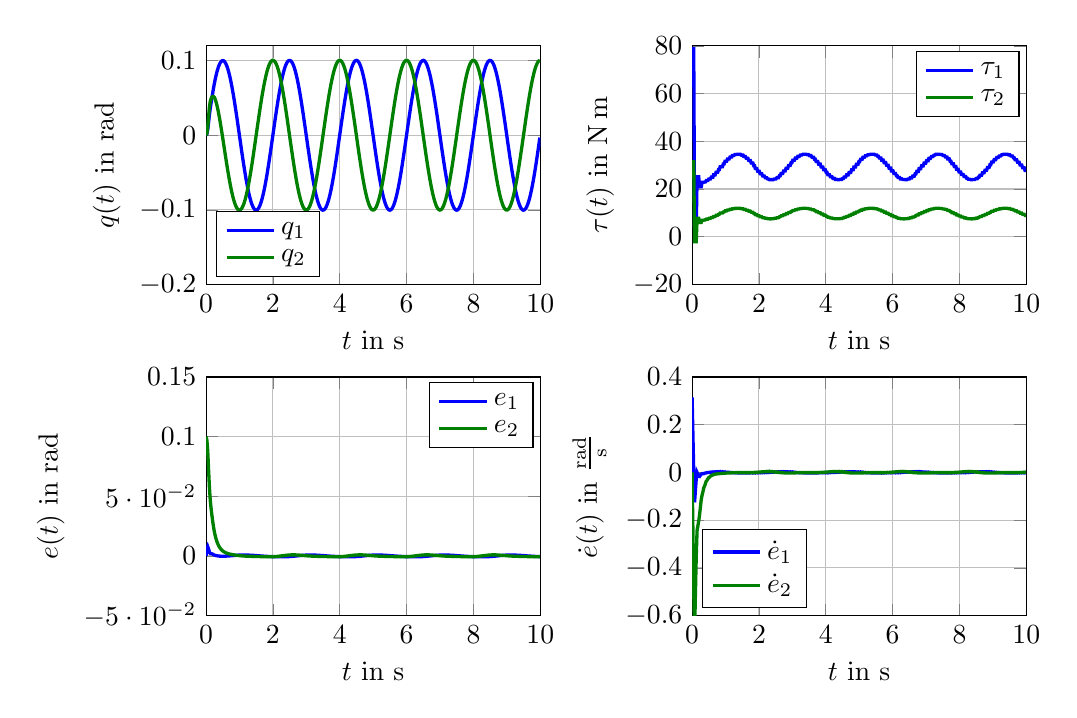
\begin{tikzpicture}

\begin{axis}[%
width=0.35\textwidth,
height=0.25\textwidth,
scale only axis,
xmin=0,
xmax=10,
xlabel={$t$ in $\mathrm{s}$},
xmajorgrids,
ymin=-0.2,
ymax=0.12,
ylabel={$q(t)$ in $\mathrm{rad}$},
ymajorgrids,
name=plot1,
legend style={at={(0.03,0.03)},anchor=south west,draw=black,fill=white,legend cell align=left}
]
\addplot [
color=blue,
solid,
line width=1.2pt
]
table[row sep=crcr]{
0 0\\
0.024133773460009 0.00182979361784962\\
0.049133773460009 0.00758473749279645\\
0.074 0.0171410959056652\\
0.099 0.0272186961721005\\
0.124 0.0358842344616407\\
0.149 0.0432117385913632\\
0.174 0.050156493820949\\
0.199 0.0569858988961169\\
0.224 0.0636303809195228\\
0.249 0.069765077730626\\
0.274 0.0753482531284275\\
0.299 0.0803866079450842\\
0.324 0.0848948216372624\\
0.349 0.0888775808125095\\
0.374 0.0922973457006214\\
0.399 0.0951098793408386\\
0.424 0.0973202878112126\\
0.449 0.0989107591658766\\
0.474 0.0998736242241424\\
0.499 0.100212943060478\\
0.523999999999997 0.0999233174847304\\
0.548999999999995 0.0990054765633401\\
0.573999999999992 0.0974658548981937\\
0.598999999999989 0.0953247877443242\\
0.623999999999986 0.0925850615022523\\
0.641550571415696 0.090310232095834\\
0.666550571415693 0.0866084525871671\\
0.691550571415691 0.0823650315013999\\
0.716499999999998 0.0776072472713715\\
0.741499999999996 0.0723802646050813\\
0.766499999999993 0.0666933772958751\\
0.79149999999999 0.0605857150924692\\
0.816499999999987 0.0541266990178515\\
0.840000000000463 0.0477298794972747\\
0.85908868789832 0.0423386213534994\\
0.884088687898318 0.0350760687192037\\
0.909088687898315 0.0275785048963679\\
0.933999999999998 0.0199360228164414\\
0.958999999999995 0.0121681302203597\\
0.983999999999992 0.00429849195958614\\
1.00899999999999 -0.00358344710708994\\
1.03399999999999 -0.0114290900086643\\
1.05899999999998 -0.0192323723074105\\
1.08399999999998 -0.0268935877615647\\
1.10899999999998 -0.0343851724060246\\
1.13399999999998 -0.0416878613319703\\
1.15899999999997 -0.0487087563008465\\
1.18399999999997 -0.0554339949847503\\
1.2017354751593 -0.0600130307236266\\
1.22673547515929 -0.0661272662336313\\
1.25173547515929 -0.0718345480762836\\
1.2765 -0.0770653382478497\\
1.3015 -0.0818584022599179\\
1.32649999999999 -0.086151459235533\\
1.35149999999999 -0.0899198097699497\\
1.37649999999999 -0.0931260595716106\\
1.40149999999998 -0.0957629134679384\\
1.42649999999998 -0.0978114217653781\\
1.45149999999998 -0.0992552563464888\\
1.47649999999998 -0.100088188916772\\
1.50149999999997 -0.100307609793127\\
1.52649999999997 -0.0999093458149972\\
1.5442337810934 -0.0992500671112728\\
1.5692337810934 -0.097804851041469\\
1.5942337810934 -0.095760052685666\\
1.619 -0.0931437956241731\\
1.644 -0.0899424448391386\\
1.66899999999999 -0.0861876402555563\\
1.69399999999999 -0.0818905020078988\\
1.71899999999999 -0.0771045435774486\\
1.74399999999999 -0.0718387723125485\\
1.76899999999998 -0.0661209523777631\\
1.79399999999998 -0.060013494460329\\
1.81899999999998 -0.0535237477426019\\
1.84399999999997 -0.0467023589057716\\
1.86899999999997 -0.0396083187556904\\
1.89000000301404 -0.0334434767860796\\
1.9117354751593 -0.0269101930399191\\
1.93673547515929 -0.0192594138032335\\
1.9615 -0.0115436757342876\\
1.9865 -0.00368744741341485\\
2.0115 0.00417884824197635\\
2.0365 0.0120454043929342\\
2.06150000000001 0.0198229896444783\\
2.08650000000002 0.0274740887007662\\
2.1115 0.0349824970391944\\
2.13650000000001 0.0422535299182929\\
2.16150000000002 0.0492681758602345\\
2.18650000000001 0.0560003708653849\\
2.21150000000001 0.062363928173118\\
2.23650000000002 0.0683543684408886\\
2.26150000000001 0.0739340408605378\\
2.28650000000002 0.0790382455217275\\
2.3115 0.0836710560537936\\
2.33650000000001 0.0877858823699699\\
2.36150000000002 0.0913474091014109\\
2.3865 0.0943600442505629\\
2.41150000000001 0.0967824808472524\\
2.43650000000002 0.0986023681194254\\
2.4615 0.0998221235840882\\
2.48650000000001 0.100419585910721\\
2.51150000000002 0.100394442325724\\
2.53650000000001 0.0997509017554698\\
2.56150000000001 0.0984920016701984\\
2.58650000000002 0.0966199648480857\\
2.61150000000001 0.094150071802681\\
2.63650000000002 0.0911060970073757\\
2.6615 0.0874873253718402\\
2.68650000000001 0.0833332711166787\\
2.71150000000002 0.0786738464874661\\
2.7365 0.073508293304517\\
2.76150000000001 0.0679054444782426\\
2.78650000000002 0.0618887781839602\\
2.8115 0.0554656893195664\\
2.83650000000001 0.0487272453857264\\
2.86150000000002 0.0416856505258469\\
2.88650000000001 0.034365520711729\\
2.91150000000001 0.0268652367108473\\
2.93650000000002 0.0191868208994927\\
2.96150000000001 0.0113796528277151\\
2.98650000000002 0.00353138644593385\\
3.0115 -0.00436080763151724\\
3.03650000000001 -0.0122198745185263\\
3.06150000000002 -0.0199843933874303\\
3.0865 -0.0276517701044\\
3.11150000000001 -0.0351308171671331\\
3.13650000000002 -0.042384978594771\\
3.1615 -0.0494011027364682\\
3.18650000000001 -0.0560914908739818\\
3.21150000000002 -0.0624365211630856\\
3.23650000000001 -0.0684125800723376\\
3.26150000000001 -0.0739489960851551\\
3.28650000000002 -0.0790353289346958\\
3.31150000000001 -0.083641758821773\\
3.33650000000002 -0.0877216526027422\\
3.3615 -0.0912678077663501\\
3.38650000000001 -0.0942525615263399\\
3.41150000000002 -0.0966524732090577\\
3.4365 -0.0984604611917408\\
3.46150000000001 -0.0996628920374431\\
3.48650000000002 -0.100250704620191\\
3.5115 -0.100219744935481\\
3.53650000000001 -0.0995765839982712\\
3.56150000000002 -0.0983189036958733\\
3.58650000000001 -0.0964514089404305\\
3.61150000000001 -0.0939996402376905\\
3.63650000000002 -0.0909637684576702\\
3.66150000000001 -0.0873647668495987\\
3.68650000000002 -0.0832396838800848\\
3.7115 -0.0785901243084186\\
3.73650000000001 -0.0734608020888883\\
3.76150000000002 -0.067888689950337\\
3.7865 -0.0618806330576769\\
3.81150000000001 -0.0555043321935716\\
3.83650000000002 -0.0487901983634562\\
3.8615 -0.0417550178792876\\
3.88650000000001 -0.034482056337176\\
3.91150000000002 -0.0269931284335131\\
3.93650000000001 -0.019319443080444\\
3.96150000000001 -0.0115489791476704\\
3.98650000000002 -0.00369491965290562\\
4.0115 0.00419255843254029\\
4.03649999999998 0.0120339063561753\\
4.06149999999997 0.0198227371644151\\
4.08649999999996 0.0274864870039897\\
4.11149999999994 0.0349675750616157\\
4.13649999999993 0.0422597793936684\\
4.16149999999991 0.0492768698464546\\
4.1864999999999 0.0559853060863905\\
4.21149999999989 0.0623740465603947\\
4.23649999999987 0.0683574815107967\\
4.26149999999986 0.0739219958739023\\
4.27972361669789 0.0777088479443076\\
4.30472361669787 0.0824666948793858\\
4.32972361669786 0.0867145569664581\\
4.35449999999999 0.0904132736281534\\
4.37949999999998 0.0935734647584362\\
4.40449999999997 0.0961587174227529\\
4.42949999999995 0.0981586047182731\\
4.45449999999994 0.0995416262117216\\
4.47949999999992 0.100312421644832\\
4.50449999999991 0.100465797587312\\
4.5294999999999 0.0999948764776919\\
4.55000005681205 0.0991454218846278\\
4.57267753810559 0.0977279683096586\\
4.59767753810557 0.0955925253702697\\
4.6225 0.092878709312507\\
4.64749999999998 0.0895793377700309\\
4.67249999999997 0.0857321325366135\\
4.69749999999996 0.0813382863410107\\
4.72249999999994 0.076457618405389\\
4.74749999999993 0.0711074181896527\\
4.77249999999992 0.0652969136783725\\
4.7974999999999 0.0591086415623467\\
4.82249999999989 0.0525508677319581\\
4.84067753810559 0.0475593465195779\\
4.86567753810558 0.0404751246398985\\
4.89067753810557 0.0331406841781521\\
4.91549999999999 0.0256325886334774\\
4.94049999999998 0.0179458037666596\\
4.96549999999996 0.010138233155836\\
4.99049999999995 0.00225467219361465\\
5.01549999999994 -0.00561284808913566\\
5.04049999999992 -0.0134654737224298\\
5.06549999999991 -0.0212327229167415\\
5.09049999999989 -0.0288486002691076\\
5.1100014203047 -0.0346848430730363\\
5.13367753810559 -0.0415908096225819\\
5.15867753810557 -0.0486128363189949\\
5.1835 -0.0553076199562839\\
5.20849999999998 -0.0617030033469733\\
5.23349999999997 -0.0677075893452699\\
5.25849999999996 -0.0733123331857254\\
5.28349999999994 -0.0784539038925142\\
5.30849999999993 -0.0831091215915823\\
5.33349999999992 -0.0872640787084309\\
5.3584999999999 -0.0908722729139573\\
5.38349999999989 -0.0939213530140675\\
5.40167753810559 -0.0957805981499437\\
5.42667753810558 -0.0978231110619888\\
5.45167753810557 -0.0992623419947073\\
5.47649999999999 -0.10008843433127\\
5.50149999999998 -0.100308084730534\\
5.52649999999996 -0.0999077648324786\\
5.55149999999995 -0.098892293683746\\
5.57649999999994 -0.0972738077009661\\
5.60149999999992 -0.095049273473229\\
5.62649999999991 -0.0922432301808132\\
5.65149999999989 -0.0888756377681306\\
5.670035507621 -0.0860159554243748\\
5.69467753810559 -0.0817688703962178\\
5.71967753810557 -0.0769706354787287\\
5.7445 -0.0717222464285272\\
5.76949999999998 -0.0660057558961969\\
5.79449999999997 -0.0598891695725402\\
5.81949999999996 -0.0533842805541015\\
5.84449999999994 -0.0465675330617901\\
5.86949999999993 -0.0394636836776011\\
5.89449999999991 -0.0320972105606091\\
5.9194999999999 -0.0245544387369563\\
5.94449999999989 -0.0168517808283934\\
5.96267753810559 -0.0111694460391063\\
5.98767753810558 -0.00332250432776343\\
6.01267753810556 0.00455121675782441\\
6.03749999999999 0.0123603001493709\\
6.06249999999998 0.0201259272424094\\
6.08749999999996 0.0277825339894541\\
6.11249999999995 0.0352769578178301\\
6.13749999999994 0.0425341342260651\\
6.16249999999992 0.0495519475569432\\
6.18749999999991 0.0562589274786119\\
6.21249999999989 0.0626072133568982\\
6.2306775381056 0.0669992272698441\\
6.25567753810559 0.0726749490834274\\
6.28067753810557 0.0778880564805479\\
6.3055 0.0826091858584095\\
6.33049999999998 0.0868462802610179\\
6.35549999999997 0.0905406446599431\\
6.38049999999996 0.0936925043957802\\
6.40549999999994 0.096253980721393\\
6.43049999999993 0.0982194364102939\\
6.45549999999991 0.0995872049041693\\
6.4804999999999 0.100332099745559\\
6.50549999999989 0.100456387653827\\
6.52367753810559 0.100158818800889\\
6.54867753810558 0.0992152006847331\\
6.57367753810556 0.0976551186113962\\
6.59849999999999 0.0955068619577856\\
6.62349999999998 0.0927628893914684\\
6.64849999999996 0.0894369416315485\\
6.67349999999995 0.0855582592970487\\
6.69849999999994 0.0811631188523473\\
6.72349999999992 0.0762487760648467\\
6.74849999999991 0.0708742311803399\\
6.77349999999989 0.065072052152146\\
6.7916775381056 0.0605815634567855\\
6.81667753810559 0.0540985322888961\\
6.84167753810557 0.0472980499762416\\
6.8665 0.0402297789666395\\
6.89149999999998 0.0328850904388619\\
6.91649999999997 0.0253461286786111\\
6.94149999999996 0.0176223595944974\\
6.96649999999994 0.0098199699773663\\
6.99149999999993 0.00195567680035262\\
7.01649999999991 -0.00594309200925262\\
7.0414999999999 -0.0137737821671917\\
7.06649999999989 -0.0215305490563155\\
7.08467753810559 -0.0271018252231976\\
7.10967753810558 -0.0345874150083205\\
7.13467753810556 -0.0418661578819667\\
7.15949999999999 -0.0488518866372137\\
7.18449999999998 -0.0555641993150257\\
7.20949999999996 -0.0619464509847098\\
7.23449999999995 -0.067949429250981\\
7.25949999999993 -0.0735193844749034\\
7.28449999999992 -0.0786500775171626\\
7.30949999999991 -0.0832911120125967\\
7.33449999999989 -0.0874131228087358\\
7.3526775381056 -0.0900804326255342\\
7.37767753810558 -0.0932653927512502\\
7.40267753810557 -0.0958715909170915\\
7.4275 -0.0978793565368061\\
7.45249999999998 -0.099300822038734\\
7.47749999999997 -0.100109697552005\\
7.50249999999996 -0.10030151704832\\
7.52749999999994 -0.0998799728358262\\
7.55249999999993 -0.0988417188811648\\
7.57749999999991 -0.09719147017312\\
7.6024999999999 -0.0949516226665892\\
7.62749999999989 -0.0921213598269805\\
7.64567753810559 -0.0897030857999086\\
7.67067753810558 -0.0859145636487537\\
7.69567753810556 -0.0815910761568935\\
7.72049999999999 -0.0767953427871767\\
7.74549999999998 -0.0715091219336567\\
7.77049999999996 -0.0657694465188729\\
7.79549999999995 -0.0596267546506661\\
7.82049999999993 -0.0531289201322042\\
7.84549999999992 -0.0462839775464755\\
7.87049999999991 -0.0391659704065839\\
7.89549999999989 -0.0318123506221305\\
7.9136775381056 -0.0263226575909197\\
7.93867753810558 -0.0186498068335827\\
7.96367753810557 -0.0108708097890081\\
7.9885 -0.00305538203208182\\
8.01350000000001 0.00481666955166633\\
8.03850000000004 0.0126582951788812\\
8.06350000000002 0.0204467266984057\\
8.08850000000005 0.0280860702077423\\
8.11350000000008 0.0355602420586308\\
8.13850000000002 0.0428334878871795\\
8.16350000000005 0.0498194283861067\\
8.18850000000008 0.0565142034154291\\
8.21350000000003 0.062866781774206\\
8.23850000000006 0.0688135675429762\\
8.26350000000001 0.0743569502269682\\
8.28850000000004 0.0794348432201572\\
8.31350000000007 0.0840128667252822\\
8.33850000000001 0.0880919725905636\\
8.36350000000004 0.0916147776535945\\
8.38850000000007 0.0945688227806819\\
8.41350000000002 0.096952052823614\\
8.43850000000005 0.0987254861885927\\
8.46350000000008 0.0998889942585132\\
8.48850000000002 0.100440928310247\\
8.51350000000005 0.100367522855911\\
8.53850000000008 0.0996720780103174\\
8.56350000000003 0.0983625341090779\\
8.58850000000006 0.0964469905858292\\
8.61350000000001 0.0939269552407247\\
8.63850000000004 0.0908328287322032\\
8.66350000000007 0.0871815515988807\\
8.68850000000001 0.082975578594862\\
8.71350000000004 0.0782729957154868\\
8.73850000000007 0.0730879418800242\\
8.76350000000002 0.0674318384864949\\
8.78850000000005 0.0613845617528144\\
8.81350000000008 0.0549518655731484\\
8.83850000000002 0.0481641014724915\\
8.86350000000005 0.0411084158553597\\
8.88850000000008 0.0337825236372234\\
8.91350000000003 0.0262447462175676\\
8.93850000000006 0.0185707867220841\\
8.96350000000001 0.0107564975816561\\
8.98850000000004 0.00288923800911719\\
9.01350000000007 -0.00498019353828145\\
9.03850000000001 -0.0128472568080688\\
9.06350000000004 -0.0206114811110482\\
9.08850000000007 -0.0282435773195426\\
9.11350000000002 -0.0357257007017169\\
9.13850000000005 -0.0429616533857046\\
9.16350000000008 -0.0499366940502546\\
9.18850000000002 -0.0566191225693929\\
9.21350000000005 -0.0629309728554459\\
9.23850000000009 -0.0688647765594971\\
9.26350000000003 -0.0743788401847901\\
9.28850000000006 -0.0794211455916952\\
9.3135 -0.0839852261611657\\
9.33850000000004 -0.0880292671136224\\
9.36350000000007 -0.0915255058246102\\
9.38850000000001 -0.0944655107757472\\
9.41350000000004 -0.0968209365126622\\
9.43850000000007 -0.0985785646298539\\
9.46350000000002 -0.0997314809626962\\
9.48850000000005 -0.100271528893937\\
9.51350000000008 -0.100192641954997\\
9.53850000000002 -0.0994958438035442\\
9.56350000000005 -0.0981924006302394\\
9.58850000000009 -0.0962792772436607\\
9.61350000000003 -0.0937736507410722\\
9.63850000000006 -0.0906988806798052\\
9.6635 -0.0870546152552691\\
9.68850000000004 -0.0828811744844997\\
9.71350000000007 -0.0782036503843028\\
9.73850000000001 -0.0730286856805827\\
9.76350000000004 -0.0674181499895861\\
9.78850000000007 -0.0613936930949332\\
9.81350000000002 -0.0549737503357852\\
9.83850000000005 -0.0482346115394166\\
9.86350000000008 -0.0411923852176581\\
9.88850000000002 -0.0338823612264938\\
9.91350000000005 -0.026384432537784\\
9.93850000000008 -0.0187091206590003\\
9.96350000000003 -0.0109136464696634\\
9.98850000000006 -0.00306824416485234\\
};
\addlegendentry{$q_1$};

\addplot [
color=green!50!black,
solid,
line width=1.2pt
]
table[row sep=crcr]{
0 0\\
0.024133773460009 0.00262475917474352\\
0.049133773460009 0.0108783319183001\\
0.074 0.0245354867825009\\
0.099 0.0372474384483777\\
0.124 0.0453670270466658\\
0.149 0.0491509861796825\\
0.174 0.0511761271507718\\
0.199 0.0521694592335697\\
0.224 0.0521048715796935\\
0.249 0.0508260744707241\\
0.274 0.048315318961395\\
0.299 0.0447273238287831\\
0.324 0.0404250589321398\\
0.349 0.0354161901670673\\
0.374 0.0298160267398526\\
0.399 0.0237592254238536\\
0.424 0.0172361262641774\\
0.449 0.0104096932573584\\
0.474 0.00336421880727148\\
0.499 -0.00389926632784047\\
0.523999999999997 -0.0112270546802228\\
0.548999999999995 -0.0185836877870833\\
0.573999999999992 -0.0259487578549939\\
0.598999999999989 -0.0331881366789882\\
0.623999999999986 -0.0402880382526726\\
0.641550571415696 -0.0451747332594085\\
0.666550571415693 -0.0519018106820167\\
0.691550571415691 -0.0583444871057118\\
0.716499999999998 -0.0644635098268108\\
0.741499999999996 -0.0702045509658639\\
0.766499999999993 -0.0755387140562451\\
0.79149999999999 -0.0804326505174296\\
0.816499999999987 -0.0848375923870498\\
0.840000000000463 -0.088517872323017\\
0.85908868789832 -0.0911634196001508\\
0.884088687898318 -0.0941390384767536\\
0.909088687898315 -0.0965439659732\\
0.933999999999998 -0.0983596356487254\\
0.958999999999995 -0.0995874671499023\\
0.983999999999992 -0.100204840350236\\
1.00899999999999 -0.100216112508571\\
1.03399999999999 -0.0996193642972657\\
1.05899999999998 -0.0984068240502392\\
1.08399999999998 -0.0966016147932822\\
1.10899999999998 -0.0942067312042066\\
1.13399999999998 -0.0912267633485744\\
1.15899999999997 -0.0876997085211728\\
1.18399999999997 -0.0836322536883619\\
1.2017354751593 -0.0804276022307225\\
1.22673547515929 -0.075503893552949\\
1.25173547515929 -0.0701149604956207\\
1.2765 -0.0643421560447689\\
1.3015 -0.0581341962086656\\
1.32649999999999 -0.0515615399431819\\
1.35149999999999 -0.0446655951917101\\
1.37649999999999 -0.0375066770661645\\
1.40149999999998 -0.0301027444200755\\
1.42649999999998 -0.0225151005018905\\
1.45149999999998 -0.014796165232444\\
1.47649999999998 -0.00696632612503538\\
1.50149999999997 0.000896739265395042\\
1.52649999999997 0.00875308772225174\\
1.5442337810934 0.014312463061347\\
1.5692337810934 0.0220586554950879\\
1.5942337810934 0.029664233175072\\
1.619 0.0370434973373858\\
1.644 0.0442495275334019\\
1.66899999999999 0.0511847979028424\\
1.69399999999999 0.0578286724363635\\
1.71899999999999 0.0640950311900961\\
1.74399999999999 0.0699756194827718\\
1.76899999999998 0.0754416896866864\\
1.79399999999998 0.0804207620724678\\
1.81899999999998 0.0849198045930488\\
1.84399999999997 0.0888993470145797\\
1.86899999999997 0.0923133842148929\\
1.89000000301404 0.0947555573431788\\
1.9117354751593 0.0968488981124067\\
1.93673547515929 0.0986812147325115\\
1.9615 0.0999059146360909\\
1.9865 0.100526152962333\\
2.0115 0.100515072733286\\
2.0365 0.0998879094952283\\
2.06150000000001 0.0986399854044601\\
2.08650000000002 0.0967768299864062\\
2.1115 0.0943113202398552\\
2.13650000000001 0.0912664541794116\\
2.16150000000002 0.0876509546975216\\
2.18650000000001 0.0834829203319796\\
2.21150000000001 0.0788130961242859\\
2.23650000000002 0.0736426823444142\\
2.26150000000001 0.0680092109069051\\
2.28650000000002 0.0619770366265872\\
2.3115 0.0555367791439727\\
2.33650000000001 0.0487615102942264\\
2.36150000000002 0.0417049567304703\\
2.3865 0.0343571654585795\\
2.41150000000001 0.0268240481405383\\
2.43650000000002 0.0191370846687432\\
2.4615 0.0112986477396963\\
2.48650000000001 0.00342881173987249\\
2.51150000000002 -0.00446089104669814\\
2.53650000000001 -0.0123469217919408\\
2.56150000000001 -0.0201178002357215\\
2.58650000000002 -0.0277728237162949\\
2.61150000000001 -0.0352655158308888\\
2.63650000000002 -0.0425108316911495\\
2.6615 -0.0495080614082017\\
2.68650000000001 -0.0561951420490594\\
2.71150000000002 -0.0625197168794432\\
2.7365 -0.0684719271305869\\
2.76150000000001 -0.0739936877457154\\
2.78650000000002 -0.0790540126140265\\
2.8115 -0.0836353505662027\\
2.83650000000001 -0.0876974386155045\\
2.86150000000002 -0.0912191134965684\\
2.88650000000001 -0.0941825666509448\\
2.91150000000001 -0.0965687175650136\\
2.93650000000002 -0.098360460402998\\
2.96150000000001 -0.0995489277896822\\
2.98650000000002 -0.100131842282624\\
3.0115 -0.10009552169711\\
3.03650000000001 -0.0994483408595929\\
3.06150000000002 -0.0981966751203088\\
3.0865 -0.0963340206053278\\
3.11150000000001 -0.0938880288101083\\
3.13650000000002 -0.0908687954031517\\
3.1615 -0.0872814210099616\\
3.18650000000001 -0.0831694019564259\\
3.21150000000002 -0.07854522591617\\
3.23650000000001 -0.0734289174303619\\
3.26150000000001 -0.0678739834084854\\
3.28650000000002 -0.0618949964057481\\
3.31150000000001 -0.05552963477891\\
3.33650000000002 -0.0488340747261214\\
3.3615 -0.0418248138971565\\
3.38650000000001 -0.0345597630372199\\
3.41150000000002 -0.0270890259855901\\
3.4365 -0.0194330359883071\\
3.46150000000001 -0.0116665229417996\\
3.48650000000002 -0.00382930467938356\\
3.5115 0.00405237852914869\\
3.53650000000001 0.011894059742565\\
3.56150000000002 0.0196682886044183\\
3.58650000000001 0.0273403949203389\\
3.61150000000001 0.0348257211198727\\
3.63650000000002 0.0421102213644084\\
3.66150000000001 0.0491467350517002\\
3.68650000000002 0.055862728254923\\
3.7115 0.0622563163608658\\
3.73650000000001 0.0682640864307568\\
3.76150000000002 0.0738389523705538\\
3.7865 0.0789841662750215\\
3.81150000000001 0.0836284553692509\\
3.83650000000002 0.0877518572170229\\
3.8615 0.0913567000234895\\
3.88650000000001 0.0943785130066152\\
3.91150000000002 0.0968184749545277\\
3.93650000000001 0.098675245007864\\
3.96150000000001 0.0999050174626518\\
3.98650000000002 0.100520686447638\\
4.0115 0.100520104094174\\
4.03649999999998 0.0998874968409209\\
4.06149999999997 0.0986372073108917\\
4.08649999999996 0.0967774583697928\\
4.11149999999994 0.094315573097731\\
4.13649999999993 0.0912613716643064\\
4.16149999999991 0.0876490176902065\\
4.1864999999999 0.0834928145068711\\
4.21149999999989 0.0788023609610637\\
4.23649999999987 0.0736428562049439\\
4.26149999999986 0.0680219056156019\\
4.27972361669789 0.0636392041372934\\
4.30472361669787 0.0573189436381751\\
4.32972361669786 0.0506435626099506\\
4.35449999999999 0.0436914765272106\\
4.37949999999998 0.0364448925706878\\
4.40449999999997 0.0289632689408794\\
4.42949999999995 0.0212847531138768\\
4.45449999999994 0.0135142722397042\\
4.47949999999992 0.00563979728191081\\
4.50449999999991 -0.00226824514979226\\
4.5294999999999 -0.0101308854759815\\
4.55000005681205 -0.0165528561788834\\
4.57267753810559 -0.0235716751485885\\
4.59767753810557 -0.0311399365613072\\
4.6225 -0.0384830542553651\\
4.64749999999998 -0.04563252277035\\
4.67249999999997 -0.0524827387450277\\
4.69749999999996 -0.0590263061395701\\
4.72249999999994 -0.0651922631375218\\
4.74749999999993 -0.0709497331047569\\
4.77249999999992 -0.0762810232318612\\
4.7974999999999 -0.081133124250904\\
4.82249999999989 -0.0854848430858795\\
4.84067753810559 -0.0883239021193952\\
4.86567753810558 -0.0917553304144265\\
4.89067753810557 -0.0946219294243219\\
4.91549999999999 -0.0968937464713923\\
4.94049999999998 -0.0985925991129587\\
4.96549999999996 -0.0996846104274308\\
4.99049999999995 -0.100164092754559\\
5.01549999999994 -0.100036053244016\\
5.04049999999992 -0.0992890319460636\\
5.06549999999991 -0.0979350816000656\\
5.09049999999989 -0.0959870880782735\\
5.1100014203047 -0.09405158122287\\
5.13367753810559 -0.0912325459828145\\
5.15867753810557 -0.0877195336348654\\
5.1835 -0.0836884606895646\\
5.20849999999998 -0.0791217444490707\\
5.23349999999997 -0.0740743057938212\\
5.25849999999996 -0.0685584876705919\\
5.28349999999994 -0.0626313246733438\\
5.30849999999993 -0.0563193954334491\\
5.33349999999992 -0.0496471252905411\\
5.3584999999999 -0.0426825008616296\\
5.38349999999989 -0.0354495311302254\\
5.40167753810559 -0.0300402291367133\\
5.42667753810558 -0.022459651354553\\
5.45167753810557 -0.0147359954693058\\
5.47649999999999 -0.00696166600757679\\
5.50149999999998 0.000895397734331773\\
5.52649999999996 0.00875900754010969\\
5.55149999999995 0.0165787897487486\\
5.57649999999994 0.0242817320985017\\
5.60149999999992 0.0318555442735907\\
5.62649999999991 0.0392317131316146\\
5.65149999999989 0.0463563722838534\\
5.670035507621 0.0514737692706865\\
5.69467753810559 0.0580020082056965\\
5.71967753810557 0.0642559751071173\\
5.7445 0.070098668518401\\
5.76949999999998 0.0755425928239116\\
5.79449999999997 0.0805131062822782\\
5.81949999999996 0.0850122709777817\\
5.84449999999994 0.0889688793996907\\
5.86949999999993 0.0923755383809531\\
5.89449999999991 0.0952312184647763\\
5.9194999999999 0.097479317725198\\
5.94449999999989 0.09912880142889\\
5.96267753810559 0.0999530337725045\\
5.98767753810558 0.100537451201519\\
6.01267753810556 0.100498827993087\\
6.03749999999999 0.0998514703233967\\
6.06249999999998 0.0985766617311839\\
6.08749999999996 0.0966883373144831\\
6.11249999999995 0.0942021718401254\\
6.13749999999994 0.0911339084892002\\
6.16249999999992 0.087489609060207\\
6.18749999999991 0.0833090725922492\\
6.21249999999989 0.0786177380477003\\
6.2306775381056 0.0748843625904316\\
6.25567753810559 0.0693604925974279\\
6.28067753810557 0.0634219357288764\\
6.3055 0.0571087505371907\\
6.33049999999998 0.050418969149326\\
6.35549999999997 0.04342769536735\\
6.38049999999996 0.0361346754273009\\
6.40549999999994 0.0286534425281276\\
6.43049999999993 0.0209964302644915\\
6.45549999999991 0.0131817197112745\\
6.4804999999999 0.00532714829850906\\
6.50549999999989 -0.00256944431049152\\
6.52367753810559 -0.00831962342059808\\
6.54867753810558 -0.0161397916393516\\
6.57367753810556 -0.023862642767006\\
6.59849999999999 -0.0314016772136544\\
6.62349999999998 -0.0387682738620607\\
6.64849999999996 -0.0459053183809329\\
6.67349999999995 -0.0527622250618354\\
6.69849999999994 -0.0592727255372033\\
6.72349999999992 -0.0654297627113868\\
6.74849999999991 -0.071178088264362\\
6.77349999999989 -0.0764791175500814\\
6.7916775381056 -0.0800451708567947\\
6.81667753810559 -0.0845202509329393\\
6.84167753810557 -0.0884707257342271\\
6.8665 -0.0918574358421476\\
6.89149999999998 -0.0947071565714806\\
6.91649999999997 -0.0969748418058477\\
6.94149999999996 -0.0986453193343585\\
6.96649999999994 -0.0997157955497199\\
6.99149999999993 -0.100173922008489\\
7.01649999999991 -0.10001359104501\\
7.0414999999999 -0.0992486094809108\\
7.06649999999989 -0.0978712370110423\\
7.08467753810559 -0.0964887949303083\\
7.10967753810558 -0.0940880740821669\\
7.13467753810556 -0.0911068484114509\\
7.15949999999999 -0.0875881201829434\\
7.18449999999998 -0.0835197875931614\\
7.20949999999996 -0.0789305240994436\\
7.23449999999995 -0.0738559196851042\\
7.25949999999993 -0.0683363319269081\\
7.28449999999992 -0.0623836804089139\\
7.30949999999991 -0.0560536414097972\\
7.33449999999989 -0.0493828683320222\\
7.3526775381056 -0.0443278762049093\\
7.37767753810558 -0.0371502950255951\\
7.40267753810557 -0.0297497915942202\\
7.4275 -0.0222022891559365\\
7.45249999999998 -0.0144749855500213\\
7.47749999999997 -0.00665848753881787\\
7.50249999999996 0.00121907038323612\\
7.52749999999994 0.00907374195377585\\
7.55249999999993 0.0168796367487072\\
7.57749999999991 0.0245990086674603\\
7.6024999999999 0.0321489743760512\\
7.62749999999989 0.0395160454399924\\
7.64567753810559 0.0447321437915284\\
7.67067753810558 0.0516443578778992\\
7.69567753810556 0.0582508912616614\\
7.72049999999999 0.0644690095991496\\
7.74549999999998 0.0703155370336585\\
7.77049999999996 0.075748371856153\\
7.79549999999995 0.0807145242964035\\
7.82049999999993 0.0851682586872086\\
7.84549999999992 0.0891194432185697\\
7.87049999999991 0.0925092950181657\\
7.89549999999989 0.0953207623052763\\
7.9136775381056 0.097010416909444\\
7.93867753810558 0.0988053515580996\\
7.96367753810557 0.0999804083859852\\
7.9885 0.100547888459644\\
8.01350000000001 0.100491444934848\\
8.03850000000004 0.0998087193963568\\
8.06350000000002 0.0985120957872694\\
8.08850000000005 0.0966031580206163\\
8.11350000000008 0.0940911340970607\\
8.13850000000002 0.0909934273826205\\
8.16350000000005 0.0873390865388125\\
8.18850000000008 0.0831320154902362\\
8.21350000000003 0.0784090693323851\\
8.23850000000006 0.0732139835757822\\
8.26350000000001 0.0675422270858344\\
8.28850000000004 0.0614652673644652\\
8.31350000000007 0.0550199239764236\\
8.33850000000001 0.0482025087169879\\
8.36350000000004 0.0411161550567611\\
8.38850000000007 0.0337803443689353\\
8.41350000000002 0.0262045629031976\\
8.43850000000005 0.0185067743004069\\
8.46350000000008 0.0106892483334304\\
8.48850000000002 0.00278519530456521\\
8.51350000000005 -0.00509551813640694\\
8.53850000000008 -0.0129600694024583\\
8.56350000000003 -0.0207475303218299\\
8.58850000000006 -0.0283759405175351\\
8.61350000000001 -0.0358499846948322\\
8.63850000000004 -0.0430901766737695\\
8.66350000000007 -0.0500477808617001\\
8.68850000000001 -0.0567149304856578\\
8.71350000000004 -0.0630163493541077\\
8.73850000000007 -0.0689233459249192\\
8.76350000000002 -0.0744171515810601\\
8.78850000000005 -0.0794415953479146\\
8.81350000000008 -0.0839765000280938\\
8.83850000000002 -0.0879996988957001\\
8.86350000000005 -0.0914783014918234\\
8.88850000000008 -0.0943944481060987\\
8.91350000000003 -0.0967328357416366\\
8.93850000000006 -0.0984793257110583\\
8.96350000000001 -0.0996178405976954\\
8.98850000000004 -0.10014926038752\\
9.01350000000007 -0.100069620798261\\
9.03850000000001 -0.099369096976181\\
9.06350000000004 -0.0980671917683193\\
9.08850000000007 -0.0961650593529475\\
9.11350000000002 -0.0936644534855963\\
9.13850000000005 -0.0906002778010164\\
9.16350000000008 -0.0869774525028967\\
9.18850000000002 -0.0828136327736832\\
9.21350000000005 -0.0781531347367125\\
9.23850000000009 -0.0730047981047558\\
9.26350000000003 -0.0674055545069335\\
9.28850000000006 -0.0614017017728233\\
9.3135 -0.055006995933039\\
9.33850000000004 -0.0482788081532549\\
9.36350000000007 -0.0412585091496752\\
9.38850000000001 -0.0339672527467394\\
9.41350000000004 -0.0264777200093831\\
9.43850000000007 -0.0188242139555069\\
9.46350000000002 -0.0110367375311296\\
9.48850000000005 -0.00319621129720858\\
9.51350000000008 0.00467194504092552\\
9.53850000000002 0.0125263514575339\\
9.56350000000005 0.0202871950408118\\
9.58850000000009 0.027939108186252\\
9.61350000000003 0.0354253020489562\\
9.63850000000006 0.042679189748734\\
9.6635 0.0496939143633322\\
9.68850000000004 0.0563957246674856\\
9.71350000000007 0.0627422072505383\\
9.73850000000001 0.0687287666962074\\
9.76350000000004 0.0742747253634782\\
9.78850000000007 0.0793619474685637\\
9.81350000000002 0.0839833710679874\\
9.83850000000005 0.088065008675946\\
9.86350000000008 0.0916087106551896\\
9.88850000000002 0.0946018877068652\\
9.91350000000005 0.0969908885611588\\
9.93850000000008 0.0987897751817979\\
9.96350000000003 0.0999822201275103\\
9.98850000000006 0.100543373088741\\
};
\addlegendentry{$q_2$};

\end{axis}

\begin{axis}[%
width=0.35\textwidth,
height=0.25\textwidth,
scale only axis,
xmin=0,
xmax=10,
xlabel={$t$ in $\mathrm{s}$},
xmajorgrids,
ymin=-0.05,
ymax=0.15,
ylabel={$e(t)$ in $\mathrm{rad}$},
ymajorgrids,
name=plot3,
at=(plot1.below south west),
anchor=above north west,
legend style={draw=black,fill=white,legend cell align=left}
]
\addplot [
color=blue,
solid,
line width=1.2pt
]
table[row sep=crcr]{
0 0\\
0.024133773460009 0.00574479303987424\\
0.049133773460009 0.00778986873465218\\
0.074 0.00589784676199383\\
0.099 0.00338406804674959\\
0.124 0.00209367509053938\\
0.149 0.0019071698528213\\
0.174 0.00182524044112192\\
0.199 0.00153817650643411\\
0.224 0.00107521523742161\\
0.249 0.000723107663610154\\
0.274 0.00048793840044474\\
0.299 0.000330034379555838\\
0.324 0.000204626542206834\\
0.349 8.00068253242608e-05\\
0.374 -3.00717136099138e-05\\
0.399 -0.000101777430761382\\
0.424 -0.000157114519745177\\
0.449 -0.000191557766394637\\
0.474 -0.00020703142073937\\
0.499 -0.000213436540291698\\
0.523999999999997 -0.000207427458668932\\
0.548999999999995 -0.000187984652311748\\
0.573999999999992 -0.000156003799980473\\
0.598999999999989 -0.000122525049755476\\
0.623999999999986 -7.7340818804908e-05\\
0.641550571415696 -3.60078920607215e-05\\
0.666550571415693 1.23182301609848e-05\\
0.691550571415691 6.82400730649679e-05\\
0.716499999999998 0.000140289358492973\\
0.741499999999996 0.000193204712527775\\
0.766499999999993 0.000258585138008194\\
0.79149999999999 0.0003319593454967\\
0.816499999999987 0.000381109704104744\\
0.840000000000463 0.000445487912769341\\
0.85908868789832 0.000498182349656755\\
0.884088687898318 0.000539085379280296\\
0.909088687898315 0.000595420329186219\\
0.933999999999998 0.000650238060547512\\
0.958999999999995 0.000676812799672268\\
0.983999999999992 0.000725939858393356\\
1.00899999999999 0.000756390430065996\\
1.03399999999999 0.000767974581142554\\
1.05899999999998 0.000802927451182163\\
1.08399999999998 0.000809437132580811\\
1.10899999999998 0.000807133466773011\\
1.13399999999998 0.000822953858342433\\
1.15899999999997 0.000808926036377902\\
1.18399999999997 0.000794560311331335\\
1.2017354751593 0.000794292616002071\\
1.22673547515929 0.000768843531405369\\
1.25173547515929 0.000739397189296373\\
1.2765 0.000719541938291546\\
1.3015 0.000680614847584901\\
1.32649999999999 0.000642168774175764\\
1.35149999999999 0.000606209469986796\\
1.37649999999999 0.000558797478677223\\
1.40149999999998 0.000512697534575501\\
1.42649999999998 0.000465501246725605\\
1.45149999999998 0.000413801213347581\\
1.47649999999998 0.000360589608156825\\
1.50149999999997 0.000308720121567671\\
1.52649999999997 0.000255692188323262\\
1.5442337810934 0.000214071192437174\\
1.5692337810934 0.000160947338901984\\
1.5942337810934 0.000110248335586718\\
1.619 5.0956312479436e-05\\
1.644 1.91968250103092e-06\\
1.66899999999999 -4.60575001751118e-05\\
1.69399999999999 -0.000104708924648089\\
1.71899999999999 -0.000146652790340221\\
1.74399999999999 -0.00019213017624535\\
1.76899999999998 -0.00024556176548679\\
1.79399999999998 -0.000279459708578525\\
1.81899999999998 -0.000323920340070186\\
1.84399999999997 -0.000368034310768775\\
1.86899999999997 -0.000394594968044226\\
1.89000000301404 -0.000430314347539235\\
1.9117354751593 -0.000464938395338305\\
1.93673547515929 -0.00048512942211194\\
1.9615 -0.000521987152862252\\
1.9865 -0.000552431332144475\\
2.0115 -0.000566802583574456\\
2.0365 -0.000603703793181865\\
2.06150000000001 -0.000622175992322983\\
2.08650000000002 -0.000632541397291905\\
2.1115 -0.000665703149254529\\
2.13650000000001 -0.000673063887703752\\
2.16150000000002 -0.000680395088982794\\
2.18650000000001 -0.000704835179008337\\
2.21150000000001 -0.000701552936748624\\
2.23650000000002 -0.000705322702679284\\
2.26150000000001 -0.000715403483060345\\
2.28650000000002 -0.000701433752076583\\
2.3115 -0.000699042386166929\\
2.33650000000001 -0.000690216859618453\\
2.36150000000002 -0.000665065488454103\\
2.3865 -0.000650109338316718\\
2.41150000000001 -0.000622707546163767\\
2.43650000000002 -0.000585613408265295\\
2.4615 -0.00055269334953062\\
2.48650000000001 -0.000509509200596628\\
2.51150000000002 -0.000459697986422036\\
2.53650000000001 -0.000407620717517307\\
2.56150000000001 -0.000352668296187963\\
2.58650000000002 -0.000289640762908397\\
2.61150000000001 -0.000222665487403115\\
2.63650000000002 -0.000160702155965406\\
2.6615 -8.46505859658231e-05\\
2.68650000000001 -1.21829507373356e-05\\
2.71150000000002 5.19528429255012e-05\\
2.7365 0.0001368464584727\\
2.76150000000001 0.000204988941207573\\
2.78650000000002 0.000267025420901887\\
2.8115 0.000352273272587321\\
2.83650000000001 0.000408739892976191\\
2.86150000000002 0.000465417750788122\\
2.88650000000001 0.000540755210267169\\
2.91150000000001 0.000581038057929514\\
2.93650000000002 0.000630237305302445\\
2.96150000000001 0.000686010059432392\\
2.98650000000002 0.00070849229961963\\
3.0115 0.000748761973114922\\
3.03650000000001 0.000778173918771823\\
3.06150000000002 0.000783579735273019\\
3.0865 0.000810222800930897\\
3.11150000000001 0.000814023277191288\\
3.13650000000002 0.00080451256417987\\
3.1615 0.000813321965220964\\
3.18650000000001 0.000795955187603579\\
3.21150000000002 0.000774145926714521\\
3.23650000000001 0.000763534334132177\\
3.26150000000001 0.000730358707676237\\
3.28650000000002 0.000698517165043572\\
3.31150000000001 0.00066974515414514\\
3.33650000000002 0.00062598709238966\\
3.3615 0.000585464153395457\\
3.38650000000001 0.000542626614093045\\
3.41150000000002 0.000492699907968505\\
3.4365 0.000443706480581771\\
3.46150000000001 0.000393461802885339\\
3.48650000000002 0.00034062791006674\\
3.5115 0.000285000596179363\\
3.53650000000001 0.000233302960319037\\
3.56150000000002 0.000179570321863193\\
3.58650000000001 0.000121084855251682\\
3.61150000000001 7.22339224133589e-05\\
3.63650000000002 1.83736062606688e-05\\
3.66150000000001 -3.79079362745893e-05\\
3.68650000000002 -8.14042858553327e-05\\
3.7115 -0.0001356750219762\\
3.73650000000001 -0.000184337674100032\\
3.76150000000002 -0.00022174346911176\\
3.7865 -0.000275170547189355\\
3.81150000000001 -0.000313630398580365\\
3.83650000000002 -0.000345786915244652\\
3.8615 -0.000396050397352084\\
3.88650000000001 -0.000424219584817948\\
3.91150000000002 -0.000453146335261449\\
3.93650000000001 -0.000497615124356188\\
3.96150000000001 -0.000516683739475094\\
3.98650000000002 -0.00054495909264574\\
4.0115 -0.00058051277413904\\
4.03649999999998 -0.000592205756429006\\
4.06149999999997 -0.000621923512272561\\
4.08649999999996 -0.000644939700534631\\
4.11149999999994 -0.000650781171694113\\
4.13649999999993 -0.000679313363103347\\
4.16149999999991 -0.00068908907523222\\
4.1864999999999 -0.00068977040004177\\
4.21149999999989 -0.000711671324056924\\
4.23649999999987 -0.000708435772622154\\
4.26149999999986 -0.000703358496456752\\
4.27972361669789 -0.000712899194222419\\
4.30472361669787 -0.000701680743183469\\
4.32972361669786 -0.000684585945913932\\
4.35449999999999 -0.000679732296565275\\
4.37949999999998 -0.000653755721902655\\
4.40449999999997 -0.000625721586422198\\
4.42949999999995 -0.00060131476942045\\
4.45449999999994 -0.000561515283971803\\
4.47949999999992 -0.000519735036281221\\
4.50449999999991 -0.000475790395335823\\
4.5294999999999 -0.000424020346680834\\
4.55000005681205 -0.000376590617162872\\
4.57267753810559 -0.00032323888472871\\
4.59767753810557 -0.000263941320225114\\
4.6225 -0.000193049748494725\\
4.64749999999998 -0.000124873786226262\\
4.67249999999997 -6.03806501037474e-05\\
4.69749999999996 2.25586090758928e-05\\
4.72249999999994 9.07029439312645e-05\\
4.74749999999993 0.00015643370288343\\
4.77249999999992 0.000243103412826962\\
4.7974999999999 0.00030346472788205\\
4.82249999999989 0.000367032365490808\\
4.84067753810559 0.000429385749407804\\
4.86567753810558 0.000482221515170279\\
4.89067753810557 0.000532760204254391\\
4.91549999999999 0.00060317154635374\\
4.94049999999998 0.000638007317603398\\
4.96549999999996 0.0006790534577803\\
4.99049999999995 0.000729397780269204\\
5.01549999999994 0.000745303639593986\\
5.04049999999992 0.000776324879616987\\
5.06549999999991 0.000800202502843531\\
5.09049999999989 0.000798681566978519\\
5.1100014203047 0.000810631226075074\\
5.13367753810559 0.000818382768312705\\
5.15867753810557 0.000801957216612942\\
5.1835 0.000799811234331503\\
5.20849999999998 0.000785328909013713\\
5.23349999999997 0.000755626911395274\\
5.25849999999996 0.000738863868126674\\
5.28349999999994 0.000706367262661295\\
5.30849999999993 0.0006668570664774\\
5.33349999999992 0.000635370263705387\\
5.3584999999999 0.000591215344141124\\
5.38349999999989 0.000544559060576211\\
5.40167753810559 0.000513411696799762\\
5.42667753810558 0.000464440930282889\\
5.45167753810557 0.00041243676084371\\
5.47649999999999 0.000360835022654771\\
5.50149999999998 0.000309195058974629\\
5.52649999999996 0.000254111205804541\\
5.55149999999995 0.000198274014767713\\
5.57649999999994 0.000147903440034153\\
5.60149999999992 9.02981177519913e-05\\
5.62649999999991 3.66373909204409e-05\\
5.65149999999989 -1.0088149825116e-05\\
5.670035507621 -5.25683590062997e-05\\
5.69467753810559 -0.000104309912062811\\
5.71967753810557 -0.00014522310017874\\
5.7445 -0.000199608434041765\\
5.76949999999998 -0.000243176172939688\\
5.79449999999997 -0.000278393006952551\\
5.81949999999996 -0.00033095950470044\\
5.84449999999994 -0.000364212159229313\\
5.86949999999993 -0.000395216889959256\\
5.89449999999991 -0.000443101977064285\\
5.9194999999999 -0.000466663923283379\\
5.94449999999989 -0.000495848536151349\\
5.96267753810559 -0.000528903248983741\\
5.98767753810558 -0.000547744400238286\\
6.01267753810556 -0.000569503555341361\\
6.03749999999999 -0.000606560403590145\\
6.06249999999998 -0.000616895040803655\\
6.08749999999996 -0.000638489002958025\\
6.11249999999995 -0.000665252110095833\\
6.13749999999994 -0.000668160472340723\\
6.16249999999992 -0.000689823407269377\\
6.18749999999991 -0.000701904176675802\\
6.21249999999989 -0.00069781842594091\\
6.2306775381056 -0.000708525872080867\\
6.25567753810559 -0.00071435367006252\\
6.28067753810557 -0.000701228051630781\\
6.3055 -0.000703993474426082\\
6.33049999999998 -0.000692223744672996\\
6.35549999999997 -0.000668892418790631\\
6.38049999999996 -0.000657145667776249\\
6.40549999999994 -0.000628609430491395\\
6.43049999999993 -0.000593614769165141\\
6.45549999999991 -0.00056282856711011\\
6.4804999999999 -0.000519686921633136\\
6.50549999999989 -0.000471315059088803\\
6.52367753810559 -0.00043534900701786\\
6.54867753810558 -0.000382226400677851\\
6.57367753810556 -0.000321977988916061\\
6.59849999999999 -0.000256646024420201\\
6.62349999999998 -0.000195627298530676\\
6.64849999999996 -0.000123341331579083\\
6.67349999999995 -4.89688356819229e-05\\
6.69849999999994 1.46685599983487e-05\\
6.72349999999992 9.70202447276858e-05\\
6.74849999999991 0.000168876804661988\\
6.77349999999989 0.000230363123325389\\
6.7916775381056 0.000291869818724845\\
6.81667753810559 0.000362506816193535\\
6.84167753810557 0.00041482454221161\\
6.8665 0.000491712891605399\\
6.89149999999998 0.000544947499569355\\
6.91649999999997 0.000586348039500393\\
6.94149999999996 0.000652673560904069\\
6.96649999999994 0.000684947958856617\\
6.99149999999993 0.000714359604375354\\
7.01649999999991 0.000761785220173683\\
7.0414999999999 0.000773076663619482\\
7.06649999999989 0.000790598510853075\\
7.08467753810559 0.000812247652721962\\
7.10967753810558 0.00080895570322144\\
7.13467753810556 0.000807072276337618\\
7.15949999999999 0.000814228535819771\\
7.18449999999998 0.000793273507504529\\
7.20949999999996 0.000779938441845707\\
7.23449999999995 0.000764441862529511\\
7.25949999999993 0.000730140029389537\\
7.28449999999992 0.000705345911472199\\
7.30949999999991 0.000671448436331726\\
7.33449999999989 0.000627904961669618\\
7.3526775381056 0.000601052216904985\\
7.37767753810558 0.00055880871111598\\
7.40267753810557 0.00050937016412661\\
7.4275 0.000462017839821416\\
7.45249999999998 0.000412172164284366\\
7.47749999999997 0.000359417910378232\\
7.50249999999996 0.000304601283840439\\
7.52749999999994 0.000252935186530495\\
7.55249999999993 0.000198793163511485\\
7.57749999999991 0.000140822826259199\\
7.6024999999999 9.1603204028734e-05\\
7.62749999999989 3.68118128638434e-05\\
7.64567753810559 -5.82521502982825e-06\\
7.67067753810558 -5.10921983331442e-05\\
7.69567753810556 -0.00010131766756355\\
7.72049999999999 -0.000155760147167255\\
7.74549999999998 -0.000194105565892624\\
7.77049999999996 -0.000243831304604925\\
7.79549999999995 -0.000289579687316681\\
7.82049999999993 -0.000321066594886975\\
7.84549999999992 -0.000370124627628053\\
7.87049999999991 -0.00040460916056545\\
7.89549999999989 -0.000430740556480437\\
7.9136775381056 -0.00046515707004768\\
7.93867753810558 -0.000496266385306501\\
7.96367753810557 -0.000515480079693596\\
7.9885 -0.00055666362632188\\
8.01350000000001 -0.000576790806106244\\
8.03850000000004 -0.000592632291720078\\
8.06350000000002 -0.000629668493598554\\
8.08850000000005 -0.000639795438947058\\
8.11350000000008 -0.000653966136609951\\
8.13850000000002 -0.000682419610532059\\
8.16350000000005 -0.000683443107385988\\
8.18850000000008 -0.000696240823252391\\
8.21350000000003 -0.000710978169331813\\
8.23850000000006 -0.000703134123509766\\
8.26350000000001 -0.000711810463976725\\
8.28850000000004 -0.000709043889755304\\
8.31350000000007 -0.000691778559327644\\
8.33850000000001 -0.00068929780468753\\
8.36350000000004 -0.000669382802176752\\
8.38850000000007 -0.000641416465395603\\
8.41350000000002 -0.000621728738433344\\
8.43850000000005 -0.00058615281457855\\
8.46350000000008 -0.0005457132205577\\
8.48850000000002 -0.000506183970944998\\
8.51350000000005 -0.000457446145786827\\
8.53850000000008 -0.000402647775763237\\
8.56350000000003 -0.000345779397920826\\
8.58850000000006 -0.000287217284746649\\
8.61350000000001 -0.000217020328479436\\
8.63850000000004 -0.000150485119253391\\
8.66350000000007 -8.58860885409457e-05\\
8.68850000000001 -3.56492723740942e-06\\
8.71350000000004 6.38160541527877e-05\\
8.73850000000007 0.00013069549743612\\
8.76350000000002 0.000217207251705417\\
8.78850000000005 0.000277813483539877\\
8.81350000000008 0.00034367011320624\\
8.83850000000002 0.000423679298748397\\
8.86350000000005 0.000472050175210841\\
8.88850000000008 0.000534270252690698\\
8.91350000000003 0.000596801085892253\\
8.93850000000006 0.000630026930049661\\
8.96350000000001 0.000685203018093918\\
8.98850000000004 0.000722807649273738\\
9.01350000000007 0.00074031479270221\\
9.03850000000001 0.000781593920915464\\
9.06350000000004 0.000794422906233369\\
9.08850000000007 0.000797302550739894\\
9.11350000000002 0.000819424779714056\\
9.13850000000005 0.000810585109050105\\
9.16350000000008 0.000800708771527124\\
9.18850000000002 0.000801159977231763\\
9.21350000000005 0.000775169250565561\\
9.23850000000009 0.000754343140024913\\
9.26350000000003 0.000733700421793826\\
9.28850000000006 0.000695346261288893\\
9.3135 0.000664137995221983\\
9.33850000000004 0.000626592327742523\\
9.36350000000007 0.000580110973189191\\
9.38850000000001 0.000538104460467287\\
9.41350000000004 0.000490612427479484\\
9.43850000000007 0.000439231255838266\\
9.46350000000002 0.000388199924742899\\
9.48850000000005 0.000336784554634456\\
9.51350000000008 0.000282565244873412\\
9.53850000000002 0.000226413568987782\\
9.56350000000005 0.000175645919083811\\
9.58850000000009 0.000119503942580271\\
9.61350000000003 6.37158288295941e-05\\
9.63850000000006 1.65370668587517e-05\\
9.6635 -4.10502550802772e-05\\
9.68850000000004 -9.08391831207084e-05\\
9.71350000000007 -0.000133161385332425\\
9.73850000000001 -0.000189951696890914\\
9.76350000000004 -0.000230895748608448\\
9.78850000000007 -0.000268682141414962\\
9.81350000000002 -0.000321785350585441\\
9.83850000000005 -0.00035316923181649\\
9.86350000000008 -0.000388080812905416\\
9.88850000000002 -0.000434432663438296\\
9.91350000000005 -0.000457114765668294\\
9.93850000000008 -0.000491692993125792\\
9.96350000000003 -0.000528054130078854\\
9.98850000000006 -0.000543801493530792\\
};
\addlegendentry{$e_1$};

\addplot [
color=green!50!black,
solid,
line width=1.2pt
]
table[row sep=crcr]{
0 0.1\\
0.024133773460009 0.0970879563482259\\
0.049133773460009 0.0879327073604713\\
0.074 0.0727743643157117\\
0.099 0.05795482424619\\
0.124 0.0471406936367799\\
0.149 0.0400918516326892\\
0.174 0.0342516160191577\\
0.199 0.0289164988496677\\
0.224 0.0241393795214513\\
0.249 0.0201063984865033\\
0.274 0.0168680535686929\\
0.299 0.0143050711068464\\
0.324 0.0120924040639898\\
0.349 0.0102625532663627\\
0.374 0.00874237248788707\\
0.399 0.00744110424498792\\
0.424 0.00641377343819508\\
0.449 0.00554396698249023\\
0.474 0.00479484234954426\\
0.499 0.00421342507642841\\
0.523999999999997 0.00369437412743033\\
0.548999999999995 0.0032506094133889\\
0.573999999999992 0.00290981518733735\\
0.598999999999989 0.00258537246014139\\
0.623999999999986 0.0023101287004965\\
0.641550571415696 0.00215654589165822\\
0.666550571415693 0.00193340003076692\\
0.691550571415691 0.00173392503881009\\
0.716499999999998 0.00157217061394396\\
0.741499999999996 0.00140708334382089\\
0.766499999999993 0.00125927729039529\\
0.79149999999999 0.00112920203585351\\
0.816499999999987 0.000999064320708912\\
0.840000000000463 0.000887204318560611\\
0.85908868789832 0.000802984405884138\\
0.884088687898318 0.000696217465499693\\
0.909088687898315 0.000594865209384177\\
0.933999999999998 0.000501545216178401\\
0.958999999999995 0.00041586113884623\\
0.983999999999992 0.000331144689633925\\
1.00899999999999 0.000256081743545092\\
1.03399999999999 0.000189285257565383\\
1.05899999999998 0.000119716237000314\\
1.08399999999998 6.34509099532721e-05\\
1.10899999999998 1.27011333252297e-05\\
1.13399999999998 -4.23953917790265e-05\\
1.15899999999997 -8.1874174943472e-05\\
1.18399999999997 -0.000120550315857434\\
1.2017354751593 -0.000152426665652169\\
1.22673547515929 -0.000181485364495512\\
1.25173547515929 -0.000209142913925264\\
1.2765 -0.000243596144544944\\
1.3015 -0.000262437519984199\\
1.32649999999999 -0.000285940659015479\\
1.35149999999999 -0.000313075325085649\\
1.37649999999999 -0.000325874904567931\\
1.40149999999998 -0.00035043874109392\\
1.42649999999998 -0.000370959848816296\\
1.45149999999998 -0.000381672135350786\\
1.47649999999998 -0.000409711845331955\\
1.50149999999997 -0.000425502111466008\\
1.52649999999997 -0.000437480777782558\\
1.5442337810934 -0.000460693774921006\\
1.5692337810934 -0.000479311906280103\\
1.5942337810934 -0.000490359112967246\\
1.619 -0.00052332114822734\\
1.644 -0.000537950868309593\\
1.66899999999999 -0.000551317167530832\\
1.69399999999999 -0.000585459876906835\\
1.71899999999999 -0.000595010247222971\\
1.74399999999999 -0.000610288901494602\\
1.76899999999998 -0.000638709796351777\\
1.79399999999998 -0.000641318118614551\\
1.81899999999998 -0.000655763377009427\\
1.84399999999997 -0.000670224371088157\\
1.86899999999997 -0.000663142024206712\\
1.89000000301404 -0.000667480127008832\\
1.9117354751593 -0.000668847275955273\\
1.93673547515929 -0.000649826836478587\\
1.9615 -0.000636484401533549\\
1.9865 -0.000616076252208178\\
2.0115 -0.00058032839398367\\
2.0365 -0.000544628457275709\\
2.06150000000001 -0.000500652030449397\\
2.08650000000002 -0.000446505901228564\\
2.1115 -0.000383913924576859\\
2.13650000000001 -0.000321059328000778\\
2.16150000000002 -0.000248279911650232\\
2.18650000000001 -0.000161832166037684\\
2.21150000000001 -8.72967938937153e-05\\
2.23650000000002 2.45741857128612e-06\\
2.26150000000001 0.00010122251254592\\
2.28650000000002 0.000178766978275721\\
2.3115 0.000281183448181975\\
2.33650000000001 0.000374474984477166\\
2.36150000000002 0.000446111546165702\\
2.3865 0.000549110463417553\\
2.41150000000001 0.000622226628239277\\
2.43650000000002 0.000679973536052831\\
2.4615 0.000767015147452253\\
2.48650000000001 0.000811067005682047\\
2.51150000000002 0.000848845388289507\\
2.53650000000001 0.000905221192187432\\
2.56150000000001 0.000916986583565003\\
2.58650000000002 0.000931276412819641\\
2.61150000000001 0.000948721940947833\\
2.63650000000002 0.000930365660559228\\
2.6615 0.000920280636955553\\
2.68650000000001 0.000899606362682111\\
2.71150000000002 0.000857341643073099\\
2.7365 0.000822881392382208\\
2.76150000000001 0.000775050368237135\\
2.78650000000002 0.000717200844374918\\
2.8115 0.000663336898575451\\
2.83650000000001 0.00060177310515247\\
2.86150000000002 0.000536769883611149\\
2.88650000000001 0.00047263173869827\\
2.91150000000001 0.000408944263924682\\
2.93650000000002 0.00034370569183767\\
2.96150000000001 0.000279497555124575\\
2.98650000000002 0.000221765572498991\\
3.0115 0.000160777357808603\\
3.03650000000001 0.000105059821640621\\
3.06150000000002 5.73417462985254e-05\\
3.0865 3.69652014868549e-06\\
3.11150000000001 -3.93775051693163e-05\\
3.13650000000002 -7.65994482582466e-05\\
3.1615 -0.000121253775912239\\
3.18650000000001 -0.000151686209514862\\
3.21150000000002 -0.000180573414220897\\
3.23650000000001 -0.000216222332627108\\
3.26150000000001 -0.000236450010964048\\
3.28650000000002 -0.000260807199113158\\
3.31150000000001 -0.000288327813242832\\
3.33650000000002 -0.00030191055258022\\
3.3615 -0.000326254379484178\\
3.38650000000001 -0.000346512884775274\\
3.41150000000002 -0.000357248783185504\\
3.4365 -0.000384022216494095\\
3.46150000000001 -0.000399139945346957\\
3.48650000000002 -0.000410574066168859\\
3.5115 -0.000440332870745311\\
3.53650000000001 -0.000452359142809467\\
3.56150000000002 -0.000467474952259964\\
3.58650000000001 -0.000498847616868747\\
3.61150000000001 -0.000508927229929693\\
3.63650000000002 -0.000529755333816273\\
3.66150000000001 -0.000558954280452044\\
3.68650000000002 -0.000567192568543873\\
3.7115 -0.0005939411244998\\
3.73650000000001 -0.000615040692550542\\
3.76150000000002 -0.000620314993074259\\
3.7865 -0.00064735450537326\\
3.81150000000001 -0.000656441701622421\\
3.83650000000002 -0.000656191706669876\\
3.8615 -0.000674356410534357\\
3.88650000000001 -0.000668578094367905\\
3.91150000000002 -0.000658701653438218\\
3.93650000000001 -0.0006584902967047\\
3.96150000000001 -0.00063558722809387\\
3.98650000000002 -0.000610609737513146\\
4.0115 -0.000585359754871825\\
4.03649999999998 -0.00054421580296761\\
4.06149999999997 -0.000497873936878515\\
4.08649999999996 -0.000447134284609824\\
4.11149999999994 -0.000388166782446048\\
4.13649999999993 -0.000315976812884616\\
4.16149999999991 -0.000246342904318908\\
4.1864999999999 -0.000171726340910824\\
4.21149999999989 -7.65616306467876e-05\\
4.23649999999987 2.28355807352365e-06\\
4.26149999999986 8.85278038833537e-05\\
4.27972361669789 0.000170073213843075\\
4.30472361669787 0.000252598492522002\\
4.32972361669786 0.000335296598591266\\
4.35449999999999 0.000443447966801694\\
4.37949999999998 0.000513566171066356\\
4.40449999999997 0.000590862860539252\\
4.42949999999995 0.000682840696904784\\
4.45449999999994 0.000731346059630584\\
4.47949999999992 0.000796016532013192\\
4.50449999999991 0.000854575546017458\\
4.5294999999999 0.000876448197708024\\
4.55000005681205 0.000909392046567901\\
4.57267753810559 0.00093721722143254\\
4.59767753810557 0.000932966123780913\\
4.6225 0.00094149713283722\\
4.64749999999998 0.000934660703242239\\
4.67249999999997 0.000904148916530838\\
4.69749999999996 0.000884987707598123\\
4.72249999999994 0.000846676664157497\\
4.74749999999993 0.00079659052768713\\
4.77249999999992 0.000752842003360232\\
4.7974999999999 0.000695560723913954\\
4.82249999999989 0.000633821587747774\\
4.84067753810559 0.000590889090002336\\
4.86567753810558 0.000527616445842011\\
4.89067753810557 0.000461963709454616\\
4.91549999999999 0.000396674558373111\\
4.94049999999998 0.000334561448936371\\
4.96549999999996 0.000271400488716517\\
4.99049999999995 0.0002086260386715\\
5.01549999999994 0.000154588441822562\\
5.04049999999992 9.73715020275712e-05\\
5.06549999999991 4.47750853976164e-05\\
5.09049999999989 1.66178446597831e-06\\
5.1100014203047 -3.63445261185591e-05\\
5.13367753810559 -7.7963863606062e-05\\
5.15867753810557 -0.000110528641427118\\
5.1835 -0.00015006737677882\\
5.20849999999998 -0.00018170403251018\\
5.23349999999997 -0.000205130972036449\\
5.25849999999996 -0.000238979951461951\\
5.28349999999994 -0.000260014539537307\\
5.30849999999993 -0.000278069350520056\\
5.33349999999992 -0.000307522873556162\\
5.3584999999999 -0.000321343665058316\\
5.38349999999989 -0.000338376757317287\\
5.40167753810559 -0.000359823253075483\\
5.42667753810558 -0.000372110517577445\\
5.45167753810557 -0.000386710480893188\\
5.47649999999999 -0.000414371962785636\\
5.50149999999998 -0.000424160580401544\\
5.52649999999996 -0.000443400595642678\\
5.55149999999995 -0.000470081495777638\\
5.57649999999994 -0.000479238080095003\\
5.60149999999992 -0.000506014780503973\\
5.62649999999991 -0.000528428437949341\\
5.65149999999989 -0.000537951009893574\\
5.670035507621 -0.000560026393644296\\
5.69467753810559 -0.000584394651946568\\
5.71967753810557 -0.000591665202446523\\
5.7445 -0.000620277682634146\\
5.76949999999998 -0.000635456984267299\\
5.79449999999997 -0.000639052840357424\\
5.81949999999996 -0.000663750033871438\\
5.84449999999994 -0.000665927634139155\\
5.86949999999993 -0.000662572855105362\\
5.89449999999991 -0.000673680108754501\\
5.9194999999999 -0.000660185206538502\\
5.94449999999989 -0.000644996895198313\\
5.96267753810559 -0.000639647847273689\\
5.98767753810558 -0.000612373394276777\\
6.01267753810556 -0.000578129636974553\\
6.03749999999999 -0.000544624627903681\\
6.06249999999998 -0.000498133690859451\\
6.08749999999996 -0.000442813669115208\\
6.11249999999995 -0.000383038247871434\\
6.13749999999994 -0.000319591106683628\\
6.16249999999992 -0.000240008352915128\\
6.18749999999991 -0.000162111361978481\\
6.21249999999989 -8.60449596051666e-05\\
6.2306775381056 -1.41889016214702e-05\\
6.25567753810559 7.77728457268811e-05\\
6.28067753810557 0.000156311471600265\\
6.3055 0.000263189124482421\\
6.33049999999998 0.000349904639428154\\
6.35549999999997 0.000425105559214572\\
6.38049999999996 0.000531685536825664\\
6.40549999999994 0.000600418165415371\\
6.43049999999993 0.000664570379396247\\
6.45549999999991 0.000752873610975032\\
6.4804999999999 0.000795126300548481\\
6.50549999999989 0.000841654327590683\\
6.52367753810559 0.000887963291735109\\
6.54867753810558 0.000906827575609056\\
6.57367753810556 0.000922291057311043\\
6.59849999999999 0.000948494052492626\\
6.62349999999998 0.000935721891338774\\
6.64849999999996 0.000926647864150226\\
6.67349999999995 0.000914744459653748\\
6.69849999999994 0.000876091808571199\\
6.72349999999992 0.000844010522092195\\
6.74849999999991 0.000801410253593676\\
6.77349999999989 0.000745409340395298\\
6.7916775381056 0.000707757732518993\\
6.81667753810559 0.000651334047159183\\
6.84167753810557 0.000587384848787689\\
6.8665 0.000524199280428739\\
6.89149999999998 0.000460498469269641\\
6.91649999999997 0.000395824150538043\\
6.94149999999996 0.00032938388557692\\
6.96649999999994 0.000269092742873525\\
6.99149999999993 0.000209573835765892\\
7.01649999999991 0.000147910954412855\\
7.0414999999999 9.7302598906529e-05\\
7.06649999999989 4.5604115712819e-05\\
7.08467753810559 6.3710844805942e-06\\
7.10967753810558 -3.42701670801027e-05\\
7.13467753810556 -7.51206900640594e-05\\
7.15949999999999 -0.000118113370513762\\
7.18449999999998 -0.00014708569720974\\
7.20949999999996 -0.000181154831948374\\
7.23449999999995 -0.000212815079394274\\
7.25949999999993 -0.000232800290520668\\
7.28449999999992 -0.000263097759774761\\
7.30949999999991 -0.000284544490574003\\
7.33449999999989 -0.000299381649608618\\
7.3526775381056 -0.000320085469592959\\
7.37767753810558 -0.000339560610423555\\
7.40267753810557 -0.000350820576677416\\
7.4275 -0.000377837530974905\\
7.45249999999998 -0.000392257839676582\\
7.47749999999997 -0.000404211054308643\\
7.50249999999996 -0.000433680294379071\\
7.52749999999994 -0.000445105374002098\\
7.55249999999993 -0.000460952091843426\\
7.57749999999991 -0.000491502584182769\\
7.6024999999999 -0.000501277657922669\\
7.62749999999989 -0.000523276661206627\\
7.64567753810559 -0.00054717706625107\\
7.67067753810558 -0.000557118622090562\\
7.69567753810556 -0.000576349293564149\\
7.72049999999999 -0.000605657375922289\\
7.74549999999998 -0.00061154026053313\\
7.77049999999996 -0.000633478852166511\\
7.79549999999995 -0.000651843355161774\\
7.82049999999993 -0.000651402860256736\\
7.84549999999992 -0.000669487026786889\\
7.87049999999991 -0.000671561854068609\\
7.89549999999989 -0.000661462332966184\\
7.9136775381056 -0.000665136870981992\\
7.93867753810558 -0.000655324149560724\\
7.96367753810557 -0.000630761164538515\\
7.9885 -0.000613144120342649\\
8.01350000000001 -0.000581368224723364\\
8.03850000000004 -0.000539289161800766\\
8.06350000000002 -0.000495341076111544\\
8.08850000000005 -0.000443384719532675\\
8.11350000000008 -0.000381199184823419\\
8.13850000000002 -0.000311083769668971\\
8.16350000000005 -0.000243421028470719\\
8.18850000000008 -0.000160001822624392\\
8.21350000000003 -7.22575627431499e-05\\
8.23850000000006 4.65380168089558e-06\\
8.26350000000001 0.000106818652368404\\
8.28850000000004 0.000197107871891679\\
8.31350000000007 0.000275611709933843\\
8.33850000000001 0.000385272054255245\\
8.36350000000004 0.000464310973812852\\
8.38850000000007 0.000536449520982626\\
8.41350000000002 0.000636984400265862\\
8.43850000000005 0.000694039351730479\\
8.46350000000008 0.000752452266296879\\
8.48850000000002 0.000826850353829798\\
8.51350000000005 0.000855639390831766\\
8.53850000000008 0.000894406515282276\\
8.56350000000003 0.000930472117019125\\
8.58850000000006 0.000929665748736236\\
8.61350000000001 0.000943708772832889\\
8.63850000000004 0.000939108397118381\\
8.66350000000007 0.000911795582975793\\
8.68850000000001 0.000896967893500113\\
8.71350000000004 0.000860545749230626\\
8.73850000000007 0.00081291250544982\\
8.76350000000002 0.000772011818066395\\
8.78850000000005 0.000715796017510581\\
8.81350000000008 0.000655411862137426\\
8.83850000000002 0.000597024109822278\\
8.86350000000005 0.000532906640404091\\
8.88850000000008 0.000467041790810918\\
8.91350000000003 0.000402511656454954\\
8.93850000000006 0.000339992337043432\\
8.96350000000001 0.000274559559742579\\
8.98850000000004 0.000214516048217567\\
9.01350000000007 0.000159544088137203\\
9.03850000000001 9.96667416240521e-05\\
9.06350000000004 5.04370571629553e-05\\
9.08850000000007 5.28605186607412e-06\\
9.11350000000002 -4.54814266477033e-05\\
9.13850000000005 -8.20658119317641e-05\\
9.16350000000008 -0.000118213007441262\\
9.18850000000002 -0.000158380893939117\\
9.21350000000005 -0.000183677032924545\\
9.23850000000009 -0.000213839272701966\\
9.26350000000003 -0.000243491231264062\\
9.28850000000006 -0.000260673463528031\\
9.3135 -0.000288539753334698\\
9.33850000000004 -0.000308972617981441\\
9.36350000000007 -0.000321956880891643\\
9.38850000000001 -0.000349541143196241\\
9.41350000000004 -0.000363827294072843\\
9.43850000000007 -0.000376599696622845\\
9.46350000000002 -0.000404963068616709\\
9.48850000000005 -0.000415834361178626\\
9.51350000000008 -0.000432066295342556\\
9.53850000000002 -0.000460688570376589\\
9.56350000000005 -0.000470136835993347\\
9.58850000000009 -0.000492833417445614\\
9.61350000000003 -0.000519026126949561\\
9.63850000000006 -0.000528121472075718\\
9.6635 -0.000557929084624958\\
9.68850000000004 -0.000577762075321703\\
9.71350000000007 -0.000586403645655674\\
9.73850000000001 -0.000618333276752286\\
9.76350000000004 -0.00062958560047921\\
9.78850000000007 -0.000636148138154824\\
9.81350000000002 -0.000662282902041622\\
9.83850000000005 -0.000662333890064315\\
9.86350000000008 -0.000663315803767009\\
9.88850000000002 -0.00067448139158402\\
9.91350000000005 -0.000660564475975081\\
9.93850000000008 -0.000650441807781482\\
9.96350000000003 -0.000638939089556589\\
9.98850000000006 -0.000608628749438941\\
};
\addlegendentry{$e_2$};

\end{axis}

\begin{axis}[%
width=0.35\textwidth,
height=0.25\textwidth,
scale only axis,
xmin=0,
xmax=10,
xlabel={$t$ in $\mathrm{s}$},
xmajorgrids,
ymin=-0.6,
ymax=0.4,
ylabel={$\dot{e}(t)$ in $\mathrm{\frac{rad}{s}}$},
ymajorgrids,
name=plot2,
at=(plot3.right of south east),
anchor=left of south west,
legend style={at={(0.03,0.03)},anchor=south west,draw=black,fill=white,legend cell align=left}
]
\addplot [
color=blue,
solid,
line width=1.2pt
]
table[row sep=crcr]{
0 0.314159265358979\\
0.024133773460009 0.161617907351022\\
0.049133773460009 0.00164251132331983\\
0.074 -0.125511743637383\\
0.099 -0.0758485453191368\\
0.124 -0.0276054481297235\\
0.149 0.000295517958558922\\
0.174 -0.0071168251420265\\
0.199 -0.0161073702390768\\
0.224 -0.0168988135939754\\
0.249 -0.0115094072712424\\
0.274 -0.00753654377441007\\
0.299 -0.00544081604074534\\
0.324 -0.00480016836076827\\
0.349 -0.00536143439663186\\
0.374 -0.00347552574369568\\
0.399 -0.00241146613901327\\
0.424 -0.00194324236421173\\
0.449 -0.000912250476790576\\
0.474 -0.00039750446240697\\
0.499 -3.51876286061536e-05\\
0.523999999999997 0.000504550226358605\\
0.548999999999995 0.00107133807641793\\
0.573999999999992 0.00128994731572601\\
0.598999999999989 0.00147275036182461\\
0.623999999999986 0.00225854876009025\\
0.641550571415696 0.00213170167044707\\
0.666550571415693 0.00190225335447053\\
0.691550571415691 0.0027688115468894\\
0.716499999999998 0.00237642229476334\\
0.741499999999996 0.00210533202877441\\
0.766499999999993 0.00339736251839895\\
0.79149999999999 0.00217436811799498\\
0.816499999999987 0.00206669638496693\\
0.840000000000463 0.00369911465228234\\
0.85908868789832 0.00201590848188166\\
0.884088687898318 0.00159838529454259\\
0.909088687898315 0.00325858427223114\\
0.933999999999998 0.00128254784165305\\
0.958999999999995 0.00119771137555669\\
0.983999999999992 0.00228823687774082\\
1.00899999999999 0.000495577993243179\\
1.03399999999999 0.000773138311968846\\
1.05899999999998 0.00107281709031748\\
1.08399999999998 -0.000230930366314885\\
1.10899999999998 0.000355214145261629\\
1.13399999999998 -1.03547289654338e-05\\
1.15899999999997 -0.000835510859809319\\
1.18399999999997 -5.51488821784463e-05\\
1.2017354751593 -0.000499848051579654\\
1.22673547515929 -0.00131180058741071\\
1.25173547515929 -0.000840626011156725\\
1.2765 -0.00126088163520263\\
1.3015 -0.00169464763964425\\
1.32649999999999 -0.00124542619558587\\
1.35149999999999 -0.00175801316786914\\
1.37649999999999 -0.00194633112601642\\
1.40149999999998 -0.00172590022869007\\
1.42649999999998 -0.00200814370536662\\
1.45149999999998 -0.00210904642619699\\
1.47649999999998 -0.00211373891646615\\
1.50149999999997 -0.0020615492451273\\
1.52649999999997 -0.00222765676516345\\
1.5442337810934 -0.00234580145369322\\
1.5692337810934 -0.00198547169223416\\
1.5942337810934 -0.00217092718555549\\
1.619 -0.00226114227633732\\
1.644 -0.00179685843966199\\
1.66899999999999 -0.00219294051913002\\
1.69399999999999 -0.00197461090032805\\
1.71899999999999 -0.00156111301934914\\
1.74399999999999 -0.00227134048699501\\
1.76899999999998 -0.00158485147026202\\
1.79399999999998 -0.00134409878773434\\
1.81899999999998 -0.0024416230988713\\
1.84399999999997 -0.00117337812681134\\
1.86899999999997 -0.00119830748588451\\
1.89000000301404 -0.00238395491363658\\
1.9117354751593 -0.000998334783205268\\
1.93673547515929 -0.000884732678721745\\
1.9615 -0.00210007589928984\\
1.9865 -0.000614297904245498\\
2.0115 -0.000820322494423653\\
2.0365 -0.00148434359081784\\
2.06150000000001 -0.000284369090744974\\
2.08650000000002 -0.00083836685105021\\
2.1115 -0.000878592413796009\\
2.13650000000001 -2.50387316019784e-06\\
2.16150000000002 -0.000874043771237176\\
2.18650000000001 -0.000281020951302391\\
2.21150000000001 0.000264984078489211\\
2.23650000000002 -0.000837001806774262\\
2.26150000000001 0.000308745908591535\\
2.28650000000002 0.000562669533689275\\
2.3115 -0.000389121105545037\\
2.33650000000001 0.000882440876518981\\
2.36150000000002 0.000936987576378806\\
2.3865 0.000624341858775648\\
2.41150000000001 0.00142232685247196\\
2.43650000000002 0.00142618329054928\\
2.4615 0.00148873446527646\\
2.48650000000001 0.00190524808375759\\
2.51150000000002 0.00204990646920678\\
2.53650000000001 0.00212193488456868\\
2.56150000000001 0.0023087459846892\\
2.58650000000002 0.00280069669812352\\
2.61150000000001 0.00247137978849726\\
2.63650000000002 0.0026165025075543\\
2.6615 0.00345973022659132\\
2.68650000000001 0.00252777953067079\\
2.71150000000002 0.00282127741823301\\
2.7365 0.00339137187284164\\
2.76150000000001 0.00232628392045084\\
2.78650000000002 0.00292454988116073\\
2.8115 0.00290249505562057\\
2.83650000000001 0.00193534483319752\\
2.86150000000002 0.00293296354384798\\
2.88650000000001 0.00213427670212873\\
2.91150000000001 0.00143764071697244\\
2.93650000000002 0.00285248499223079\\
2.96150000000001 0.00124145071872828\\
2.98650000000002 0.000909427636982929\\
3.0115 0.00233313875870544\\
3.03650000000001 0.000360078642682615\\
3.06150000000002 0.000404222385269049\\
3.0865 0.00102406083832479\\
3.11150000000001 -0.000413552261255168\\
3.13650000000002 -5.54590771295604e-05\\
3.1615 -0.000102690945414485\\
3.18650000000001 -0.00103034782398276\\
3.21150000000002 -0.000477324910450022\\
3.23650000000001 -0.000975482388707455\\
3.26150000000001 -0.00148395818540401\\
3.28650000000002 -0.000890921420202612\\
3.31150000000001 -0.00157561121110761\\
3.33650000000002 -0.00179880403289026\\
3.3615 -0.00142523152245178\\
3.38650000000001 -0.00192270880007779\\
3.41150000000002 -0.00201564877336978\\
3.4365 -0.001949847200485\\
3.46150000000001 -0.00206007273146234\\
3.48650000000002 -0.00217922142269576\\
3.5115 -0.00214784263371267\\
3.53650000000001 -0.00204319654972954\\
3.56150000000002 -0.00233088708380078\\
3.58650000000001 -0.00208856551660667\\
3.61150000000001 -0.00193239508968143\\
3.63650000000002 -0.00250706393098937\\
3.66150000000001 -0.00185318882243185\\
3.68650000000002 -0.00178849125987779\\
3.7115 -0.00255645984892319\\
3.73650000000001 -0.00152555869122245\\
3.76150000000002 -0.00166937795989766\\
3.7865 -0.00211809913072003\\
3.81150000000001 -0.00118264317885208\\
3.83650000000002 -0.00162513529079483\\
3.8615 -0.00162047084061173\\
3.88650000000001 -0.000885142862211863\\
3.91150000000002 -0.00169027873905631\\
3.93650000000001 -0.00112996030927254\\
3.96150000000001 -0.000669443761348254\\
3.98650000000002 -0.00187329834004696\\
4.0115 -0.000682026357610388\\
4.03649999999998 -0.000542039300913288\\
4.06149999999997 -0.0018499662917516\\
4.08649999999996 -0.000283856542334149\\
4.11149999999994 -0.000477178230132991\\
4.13649999999993 -0.001149949362239\\
4.16149999999991 7.84645188979249e-05\\
4.1864999999999 -0.000418353782395298\\
4.21149999999989 -0.000442332502578635\\
4.23649999999987 0.000431211547121224\\
4.26149999999986 -0.000284549300328119\\
4.27972361669789 -0.000130559546928199\\
4.30472361669787 0.000793025667278735\\
4.32972361669786 0.000356465378417076\\
4.35449999999999 0.000656374984175173\\
4.37949999999998 0.00124513717449666\\
4.40449999999997 0.000844725279645311\\
4.42949999999995 0.00136951856921001\\
4.45449999999994 0.00171576457117779\\
4.47949999999992 0.00155724819113495\\
4.50449999999991 0.00193698729524501\\
4.5294999999999 0.00219778998241706\\
4.55000005681205 0.00244469549320397\\
4.57267753810559 0.00230199155808616\\
4.59767753810557 0.00252330821002107\\
4.6225 0.00310416158734265\\
4.64749999999998 0.00249397467462323\\
4.67249999999997 0.00284003239963468\\
4.69749999999996 0.00324511454170545\\
4.72249999999994 0.00243554479676769\\
4.74749999999993 0.00307736355064514\\
4.77249999999992 0.00295045583541653\\
4.7974999999999 0.0021739044380758\\
4.82249999999989 0.003224936442423\\
4.84067753810559 0.00283413516854075\\
4.86567753810558 0.00172743615724374\\
4.89067753810557 0.00266053948568107\\
4.91549999999999 0.00197688892436998\\
4.94049999999998 0.00116328224177448\\
4.96549999999996 0.00247528915503398\\
4.99049999999995 0.0010241520067848\\
5.01549999999994 0.000595186615202248\\
5.04049999999992 0.00211649495936611\\
5.06549999999991 0.000123066814172124\\
5.09049999999989 7.36130763919762e-05\\
5.1100014203047 0.00133831084168917\\
5.13367753810559 -0.000421159395659398\\
5.15867753810557 -0.000616091428234045\\
5.1835 0.000193195296725568\\
5.20849999999998 -0.00111274486050109\\
5.23349999999997 -0.00104458311634073\\
5.25849999999996 -0.000820952795723612\\
5.28349999999994 -0.00160383282300045\\
5.30849999999993 -0.00140467475178202\\
5.33349999999992 -0.00151682569216083\\
5.3584999999999 -0.00191004130312786\\
5.38349999999989 -0.00174039468325735\\
5.40167753810559 -0.00182647579774328\\
5.42667753810558 -0.00204960183003848\\
5.45167753810557 -0.00209207204455304\\
5.47649999999999 -0.00205881348319954\\
5.50149999999998 -0.00209807449638135\\
5.52649999999996 -0.00235564774361483\\
5.55149999999995 -0.00205202936489467\\
5.57649999999994 -0.00206465804827581\\
5.60149999999992 -0.00254014333951143\\
5.62649999999991 -0.00187590803762547\\
5.65149999999989 -0.00200243992938556\\
5.670035507621 -0.00266238499171623\\
5.69467753810559 -0.00169861157179618\\
5.71967753810557 -0.00175538409243642\\
5.7445 -0.00232670687274614\\
5.76949999999998 -0.00136404278713467\\
5.79449999999997 -0.00167112419207416\\
5.81949999999996 -0.0018546593066886\\
5.84449999999994 -0.0010427117614592\\
5.86949999999993 -0.00168520964513713\\
5.89449999999991 -0.00135926588605712\\
5.9194999999999 -0.000788207648793671\\
5.94449999999989 -0.00181727804997223\\
5.96267753810559 -0.00125771573997535\\
5.98767753810558 -0.000529254752056008\\
6.01267753810556 -0.00149703933944428\\
6.03749999999999 -0.000772456394170673\\
6.06249999999998 -0.000345764793602543\\
6.08749999999996 -0.00167559331960399\\
6.11249999999995 -0.000312968156148286\\
6.13749999999994 -0.00021212952878441\\
6.16249999999992 -0.00137298844219258\\
6.18749999999991 0.000121877696127537\\
6.21249999999989 -7.35096269724456e-05\\
6.2306775381056 -0.00112983894989246\\
6.25567753810559 0.000401814454299126\\
6.28067753810557 0.000398751171781786\\
6.3055 -0.000185379084430837\\
6.33049999999998 0.000909734725801525\\
6.35549999999997 0.000758972888447007\\
6.38049999999996 0.0007219462996811\\
6.40549999999994 0.00140938306847799\\
6.43049999999993 0.00126456001132289\\
6.45549999999991 0.00150026912592169\\
6.4804999999999 0.00188304096259715\\
6.50549999999989 0.00194939273955443\\
6.52367753810559 0.00203437109624013\\
6.54867753810558 0.00223327156685245\\
6.57367753810556 0.00263711477771039\\
6.59849999999999 0.00246022071032168\\
6.62349999999998 0.00253572702244316\\
6.64849999999996 0.00339330302552437\\
6.67349999999995 0.00257303278774956\\
6.69849999999994 0.00272199396638101\\
6.72349999999992 0.00360214574997261\\
6.74849999999991 0.00240079691319578\\
6.77349999999989 0.00279541323675178\\
6.7916775381056 0.00381651358798291\\
6.81667753810559 0.00214273209956933\\
6.84167753810557 0.00236664317000501\\
6.8665 0.00305755621061327\\
6.89149999999998 0.00154505132102439\\
6.91649999999997 0.00211793565517876\\
6.94149999999996 0.00205497868375698\\
6.96649999999994 0.000880552660026512\\
6.99149999999993 0.00182462540961409\\
7.01649999999991 0.00100101515178336\\
7.0414999999999 0.000241387199552079\\
7.06649999999989 0.00149057047729817\\
7.08467753810559 0.000448514738196959\\
7.10967753810558 -0.000404154690131775\\
7.13467753810556 0.000546673335160452\\
7.15949999999999 -0.000484153566713774\\
7.18449999999998 -0.000934300137772959\\
7.20949999999996 0.000106254193576738\\
7.23449999999995 -0.00120272854442077\\
7.25949999999993 -0.00134498109560904\\
7.28449999999992 -0.000872078673316123\\
7.30949999999991 -0.00168853247811751\\
7.33449999999989 -0.00166681071991903\\
7.3526775381056 -0.00138274648698883\\
7.37767753810558 -0.00190935663796289\\
7.40267753810557 -0.0019816898183673\\
7.4275 -0.0019112590657215\\
7.45249999999998 -0.00205857308080276\\
7.47749999999997 -0.00216637882273058\\
7.50249999999996 -0.00212300879483515\\
7.52749999999994 -0.00205805951986924\\
7.55249999999993 -0.00234161463815532\\
7.57749999999991 -0.00207929884489293\\
7.6024999999999 -0.00196469311057562\\
7.62749999999989 -0.00254311150180991\\
7.64567753810559 -0.00202389189254404\\
7.67067753810558 -0.00174970417905201\\
7.69567753810556 -0.00243624041650148\\
7.72049999999999 -0.00170119345031125\\
7.74549999999998 -0.00156076757433327\\
7.77049999999996 -0.00255483138938506\\
7.79549999999995 -0.00132189477303452\\
7.82049999999993 -0.00142567502511831\\
7.84549999999992 -0.00204402714954599\\
7.87049999999991 -0.000961055715606673\\
7.89549999999989 -0.0013854810436657\\
7.9136775381056 -0.00202088248078841\\
7.93867753810558 -0.000735172639221016\\
7.96367753810557 -0.00107696477785935\\
7.9885 -0.00146231130625751\\
8.01350000000001 -0.000432328095548273\\
8.03850000000004 -0.0011243318352368\\
8.06350000000002 -0.000910909138986948\\
8.08850000000005 -0.000192273763863549\\
8.11350000000008 -0.00123536784816836\\
8.13850000000002 -0.00038231010363915\\
8.16350000000005 1.10467407495873e-05\\
8.18850000000008 -0.00132002859220154\\
8.21350000000003 0.000131623769736994\\
8.23850000000006 0.00022655648709885\\
8.26350000000001 -0.000661540963372287\\
8.28850000000004 0.000638001194188137\\
8.31350000000007 0.000513790569022954\\
8.33850000000001 0.000264939096639466\\
8.36350000000004 0.00113743316242779\\
8.38850000000007 0.000931468344014114\\
8.41350000000002 0.00110638785635461\\
8.43850000000005 0.00162299118993896\\
8.46350000000008 0.0015237911532529\\
8.48850000000002 0.00178981651955261\\
8.51350000000005 0.00208200575910038\\
8.53850000000008 0.00230664003702883\\
8.56350000000003 0.00225571762901061\\
8.58850000000006 0.00249888379626818\\
8.61350000000001 0.00298167160671976\\
8.63850000000004 0.00247413485955292\\
8.66350000000007 0.00285772029270565\\
8.68850000000001 0.00315808137409743\\
8.71350000000004 0.00245218993607951\\
8.73850000000007 0.00314407291533286\\
8.76350000000002 0.00290644196965653\\
8.78850000000005 0.00223080169390585\\
8.81350000000008 0.00334544071990278\\
8.83850000000002 0.00233157336156703\\
8.86350000000005 0.00187219555118823\\
8.88850000000008 0.00345004159360085\\
8.91350000000003 0.00156892643171985\\
8.93850000000006 0.00144263329341987\\
8.96350000000001 0.00260725993162847\\
8.98850000000004 0.000752476777843791\\
9.01350000000007 0.000995752295861074\\
9.03850000000001 0.00136781691663385\\
9.06350000000004 -1.10630444149495e-05\\
9.08850000000007 0.000561036859329733\\
9.11350000000002 0.000239393747101968\\
9.13850000000005 -0.000656405538581706\\
9.16350000000008 0.000139958890179093\\
9.18850000000002 -0.000682584247304885\\
9.21350000000005 -0.0011614362558989\\
9.23850000000009 -0.00028993793087384\\
9.26350000000003 -0.00135858988958282\\
9.28850000000006 -0.00153918975228046\\
9.3135 -0.00108630765496456\\
9.33850000000004 -0.00179312902065171\\
9.36350000000007 -0.001824484878094\\
9.38850000000001 -0.00172581667206587\\
9.41350000000004 -0.00201972867684483\\
9.43850000000007 -0.00206002955424291\\
9.46350000000002 -0.00204014266781069\\
9.48850000000005 -0.00208745584957906\\
9.51350000000008 -0.00228610563348023\\
9.53850000000002 -0.00208687126285933\\
9.56350000000005 -0.00205147918369049\\
9.58850000000009 -0.00253623822397443\\
9.61350000000003 -0.00193802399252925\\
9.63850000000006 -0.00196793624543498\\
9.6635 -0.00247380685229195\\
9.68850000000004 -0.00167197916529022\\
9.71350000000007 -0.00189147191225608\\
9.73850000000001 -0.00211266645892716\\
9.76350000000004 -0.00136553016806509\\
9.78850000000007 -0.00187271828403218\\
9.81350000000002 -0.00166034938582338\\
9.83850000000005 -0.00108546188686848\\
9.86350000000008 -0.00195308871692024\\
9.88850000000002 -0.00119555801784488\\
9.91350000000005 -0.000879972144561092\\
9.93850000000008 -0.00215558311533787\\
9.96350000000003 -0.000769270624518426\\
9.98850000000006 -0.000770889589051804\\
};
\addlegendentry{$\dot{e}_1$};

\addplot [
color=green!50!black,
solid,
line width=1.2pt
]
table[row sep=crcr]{
0 -0\\
0.024133773460009 -0.241311490879811\\
0.049133773460009 -0.491025449113072\\
0.074 -0.673046750340015\\
0.099 -0.512579165520159\\
0.124 -0.352651608454598\\
0.149 -0.243513122814513\\
0.174 -0.223614673009144\\
0.199 -0.203069907082082\\
0.224 -0.176796857679487\\
0.249 -0.145645889574746\\
0.274 -0.113178677886201\\
0.299 -0.0955064701275243\\
0.324 -0.0811864007869641\\
0.349 -0.0648507525798194\\
0.374 -0.056808438671545\\
0.399 -0.0469004306539546\\
0.424 -0.0363814715893904\\
0.449 -0.0327912300306882\\
0.474 -0.0267262913868709\\
0.499 -0.021479374979763\\
0.523999999999997 -0.0196469450751933\\
0.548999999999995 -0.0154715764054097\\
0.573999999999992 -0.013291931918941\\
0.598999999999989 -0.012322102976002\\
0.623999999999986 -0.0093826642991488\\
0.641550571415696 -0.00888132936750385\\
0.666550571415693 -0.00870340340224435\\
0.691550571415691 -0.00701992615617175\\
0.716499999999998 -0.00661991851674437\\
0.741499999999996 -0.00641411134485131\\
0.766499999999993 -0.00527093334741977\\
0.79149999999999 -0.00529054792007447\\
0.816499999999987 -0.00503873004410871\\
0.840000000000463 -0.00443520946823231\\
0.85908868789832 -0.00436851984588649\\
0.884088687898318 -0.00416121974307572\\
0.909088687898315 -0.00396065348399093\\
0.933999999999998 -0.00354783807648524\\
0.958999999999995 -0.0033563968496445\\
0.983999999999992 -0.00333093730186487\\
1.00899999999999 -0.00275191416140026\\
1.03399999999999 -0.00268423747019508\\
1.05899999999998 -0.00258738420876017\\
1.08399999999998 -0.0020245335556143\\
1.10899999999998 -0.00215603294486905\\
1.13399999999998 -0.00186369528422992\\
1.15899999999997 -0.00142709766316004\\
1.18399999999997 -0.00180631551934488\\
1.2017354751593 -0.00148713689871158\\
1.22673547515929 -0.000984497957009334\\
1.25173547515929 -0.00138070949405877\\
1.2765 -0.000987625669816611\\
1.3015 -0.000681855582226165\\
1.32649999999999 -0.0013662484449023\\
1.35149999999999 -0.00063632501694133\\
1.37649999999999 -0.00056721567529866\\
1.40149999999998 -0.00140676630567366\\
1.42649999999998 -0.000427834161084106\\
1.45149999999998 -0.000629874603456981\\
1.47649999999998 -0.00114541713447525\\
1.50149999999997 -0.000334455242675058\\
1.52649999999997 -0.000848931317876667\\
1.5442337810934 -0.00137957402370864\\
1.5692337810934 -0.000349554551814846\\
1.5942337810934 -0.000781829114892774\\
1.619 -0.00113896798310009\\
1.644 -0.000294310402762454\\
1.66899999999999 -0.0010429446383533\\
1.69399999999999 -0.000821658425131322\\
1.71899999999999 -0.00021948316080303\\
1.74399999999999 -0.00127938994019366\\
1.76899999999998 -0.000411520661319026\\
1.79399999999998 -7.11247324722275e-05\\
1.81899999999998 -0.00134983047494691\\
1.84399999999997 0.000104345260994065\\
1.86899999999997 0.000216561898090439\\
1.89000000301404 -0.00079118011194465\\
1.9117354751593 0.000500173153784422\\
1.93673547515929 0.000826488582472737\\
1.9615 0.000239048875531882\\
1.9865 0.00124977687017933\\
2.0115 0.00150096982517718\\
2.0365 0.00149777946458574\\
2.06150000000001 0.00198106358139944\\
2.08650000000002 0.00235283896386537\\
2.1115 0.00250391202908584\\
2.13650000000001 0.00260763330344377\\
2.16150000000002 0.00334151814467762\\
2.18650000000001 0.003113304122349\\
2.21150000000001 0.00305752453140615\\
2.23650000000002 0.00437093408274616\\
2.26150000000001 0.00324883327501616\\
2.28650000000002 0.00327184630705463\\
2.3115 0.00492051645263752\\
2.33650000000001 0.00291509521425753\\
2.36150000000002 0.0032096501355473\\
2.3865 0.0040768909163319\\
2.41150000000001 0.00219309562197323\\
2.43650000000002 0.00285337690215132\\
2.4615 0.00272770238035358\\
2.48650000000001 0.00121870086248727\\
2.51150000000002 0.00221624268869575\\
2.53650000000001 0.00116919222853429\\
2.56150000000001 0.000152038708322644\\
2.58650000000002 0.00134856039465886\\
2.61150000000001 -0.000309406925251277\\
2.63650000000002 -0.000854377519149851\\
2.6615 7.80325007663785e-05\\
2.68650000000001 -0.00148716488738643\\
2.71150000000002 -0.00168230458628985\\
2.7365 -0.00143044696691957\\
2.76150000000001 -0.00224663127230515\\
2.78650000000002 -0.00226470442505219\\
2.8115 -0.00228683805957766\\
2.83650000000001 -0.00257755352226319\\
2.86150000000002 -0.00259081497213265\\
2.88650000000001 -0.00255298880344026\\
2.91150000000001 -0.00255446921106867\\
2.93650000000002 -0.00269997395593542\\
2.96150000000001 -0.00238497742984887\\
2.98650000000002 -0.00230043202612241\\
3.0115 -0.00257762526731768\\
3.03650000000001 -0.00197100405495857\\
3.06150000000002 -0.00195034423878234\\
3.0865 -0.00208335360426674\\
3.11150000000001 -0.00148204191649784\\
3.13650000000002 -0.00162376127216213\\
3.1615 -0.00152869727351315\\
3.18650000000001 -0.00104455645063398\\
3.21150000000002 -0.00141127710647282\\
3.23650000000001 -0.00103741908636695\\
3.26150000000001 -0.000734858687302997\\
3.28650000000002 -0.00137325106572742\\
3.31150000000001 -0.000668341642477199\\
3.33650000000002 -0.000588235229390666\\
3.3615 -0.00136805467122197\\
3.38650000000001 -0.000434464117715361\\
3.41150000000002 -0.000613401473794462\\
3.4365 -0.0010898018041568\\
3.46150000000001 -0.00032327096018453\\
3.48650000000002 -0.000803280938123707\\
3.5115 -0.000880556022588297\\
3.53650000000001 -0.00031009837025181\\
3.56150000000002 -0.00113594692149011\\
3.58650000000001 -0.000698154293075459\\
3.61150000000001 -0.000361506975479653\\
3.63650000000002 -0.00156445249437781\\
3.66150000000001 -0.000500507048020349\\
3.68650000000002 -0.000430628749530426\\
3.7115 -0.00171829416823308\\
3.73650000000001 -0.000248968638958152\\
3.76150000000002 -0.000450144158924276\\
3.7865 -0.00108778779148888\\
3.81150000000001 8.94483410431857e-05\\
3.83650000000002 -0.00032985833823565\\
3.8615 -0.000313517893625881\\
3.88650000000001 0.000539289815990454\\
3.91150000000002 3.55096815210371e-05\\
3.93650000000001 0.000548862299606413\\
3.96150000000001 0.00111281422160898\\
3.98650000000002 0.00074600373653134\\
4.0115 0.00141163450289468\\
4.03649999999998 0.00180493422634109\\
4.06149999999997 0.00188564914084127\\
4.08649999999996 0.00217311158228187\\
4.11149999999994 0.00258683424136653\\
4.13649999999993 0.00295734249125598\\
4.16149999999991 0.00273834000416176\\
4.1864999999999 0.0033991298944154\\
4.21149999999989 0.00351836025114169\\
4.23649999999987 0.00303599328700027\\
4.26149999999986 0.00414788364932439\\
4.27972361669789 0.00398961956648611\\
4.30472361669787 0.00295133560104816\\
4.32972361669786 0.00403110112139032\\
4.35449999999999 0.00347954833959396\\
4.37949999999998 0.00253559033262563\\
4.40449999999997 0.00406698006129219\\
4.42949999999995 0.00247063385245283\\
4.45449999999994 0.00183712940273617\\
4.47949999999992 0.00376102179552484\\
4.50449999999991 0.0011995397123673\\
4.5294999999999 0.000953029855687793\\
4.55000005681205 0.00252128515137817\\
4.57267753810559 0.000237132905276383\\
4.59767753810557 -0.0002303952523936\\
4.6225 0.000769630794772047\\
4.64749999999998 -0.00102398820791388\\
4.67249999999997 -0.00115585909141863\\
4.69749999999996 -0.000916147583883753\\
4.72249999999994 -0.0019499712976625\\
4.74749999999993 -0.00189176475923461\\
4.77249999999992 -0.00200770870208059\\
4.7974999999999 -0.0024697367393933\\
4.82249999999989 -0.00239570905609357\\
4.84067753810559 -0.00243600472707095\\
4.86567753810558 -0.00259546039966926\\
4.89067753810557 -0.00265297285417404\\
4.91549999999999 -0.00254476923828297\\
4.94049999999998 -0.00245971406954039\\
4.96549999999996 -0.00264895639970392\\
4.99049999999995 -0.00227057877470764\\
5.01549999999994 -0.00213518214097157\\
5.04049999999992 -0.00250580216600053\\
5.06549999999991 -0.00180526419145334\\
5.09049999999989 -0.00175803934121074\\
5.1100014203047 -0.00221436644294508\\
5.13367753810559 -0.00141391317962017\\
5.15867753810557 -0.00132428892249309\\
5.1835 -0.0017186039945831\\
5.20849999999998 -0.000955280415465415\\
5.23349999999997 -0.00106777974529934\\
5.25849999999996 -0.00122040687506172\\
5.28349999999994 -0.000620639270837942\\
5.30849999999993 -0.000987707816442029\\
5.33349999999992 -0.000841848420603308\\
5.3584999999999 -0.000438826493837641\\
5.38349999999989 -0.00110529394132697\\
5.40167753810559 -0.000835411713088707\\
5.42667753810558 -0.000340749842102694\\
5.45167753810557 -0.00102802811874875\\
5.47649999999999 -0.000640182657217159\\
5.50149999999998 -0.000359660648965698\\
5.52649999999996 -0.00140451351545873\\
5.55149999999995 -0.000497817242324894\\
5.57649999999994 -0.00047670778187725\\
5.60149999999992 -0.00167384248068075\\
5.62649999999991 -0.000377379777465048\\
5.65149999999989 -0.000648644661751463\\
5.670035507621 -0.00187418169394521\\
5.69467753810559 -0.000370503366912245\\
5.71967753810557 -0.000487585287788028\\
5.7445 -0.00139348918069385\\
5.76949999999998 -9.94717593320038e-05\\
5.79449999999997 -0.000461056225847523\\
5.81949999999996 -0.000709560836170076\\
5.84449999999994 0.000275762012043268\\
5.86949999999993 -0.000251617686772398\\
5.89449999999991 9.5958663450621e-05\\
5.9194999999999 0.000772359501164194\\
5.94449999999989 0.000257124368215525\\
5.96267753810559 0.000686708040879579\\
5.98767753810558 0.00135428361938966\\
6.01267753810556 0.00127873851703961\\
6.03749999999999 0.0016303094974506\\
6.06249999999998 0.00205233352094956\\
6.08749999999996 0.0023778369984018\\
6.11249999999995 0.00240192503079362\\
6.13749999999994 0.00275947817379918\\
6.16249999999992 0.00351005077103711\\
6.18749999999991 0.00288992474262958\\
6.21249999999989 0.00340552336912789\\
6.2306775381056 0.00451420325688226\\
6.25567753810559 0.0031174532498642\\
6.28067753810557 0.00347543320558338\\
6.3055 0.00444379646925724\\
6.33049999999998 0.00285998068398924\\
6.35549999999997 0.00354544267133999\\
6.38049999999996 0.00368214001701528\\
6.40549999999994 0.00223499101998637\\
6.43049999999993 0.00332315820471446\\
6.45549999999991 0.00244853179014665\\
6.4804999999999 0.00135549918474154\\
6.50549999999989 0.00278226186771163\\
6.52367753810559 0.00159258120878047\\
6.54867753810558 0.000306535541852226\\
6.57367753810556 0.0012998587347603\\
6.59849999999999 3.9579054838923e-05\\
6.62349999999998 -0.000741786355244689\\
6.64849999999996 0.000305508477430327\\
6.67349999999995 -0.0012520321469095\\
6.69849999999994 -0.0016116589491707\\
6.72349999999992 -0.00112069077106106\\
6.74849999999991 -0.00212142365656298\\
6.77349999999989 -0.00222580365729419\\
6.7916775381056 -0.00195438162367315\\
6.81667753810559 -0.00247599923741876\\
6.84167753810557 -0.00258623279289708\\
6.8665 -0.00252876663558679\\
6.89149999999998 -0.00256126122401192\\
6.91649999999997 -0.00263094415589493\\
6.94149999999996 -0.00254292954900313\\
6.96649999999994 -0.00233368586580474\\
6.99149999999993 -0.0024992208371401\\
7.01649999999991 -0.00219835279810612\\
7.0414999999999 -0.00194503682000041\\
7.06649999999989 -0.00229801958272456\\
7.08467753810559 -0.00186486405540358\\
7.10967753810558 -0.00150591872293269\\
7.13467753810556 -0.00189023021382118\\
7.15949999999999 -0.00133731563627523\\
7.18449999999998 -0.00111907342333595\\
7.20949999999996 -0.00175120090075584\\
7.23449999999995 -0.000882117723750436\\
7.25949999999993 -0.000870579583072989\\
7.28449999999992 -0.00132031859260423\\
7.30949999999991 -0.000559047444649352\\
7.33449999999989 -0.00079752205808109\\
7.3526775381056 -0.0013059601387746\\
7.37767753810558 -0.000431626968971588\\
7.40267753810557 -0.000655729660212434\\
7.4275 -0.00103193114022748\\
7.45249999999998 -0.000322559579600923\\
7.47749999999997 -0.000842606393965162\\
7.50249999999996 -0.000823757899810373\\
7.52749999999994 -0.00031574096614595\\
7.55249999999993 -0.00118575607104493\\
7.57749999999991 -0.000650968739647206\\
7.6024999999999 -0.000381509409114189\\
7.62749999999989 -0.00163561087739217\\
7.64567753810559 -0.000752121559720154\\
7.67067753810558 -0.000312394638419755\\
7.69567753810556 -0.00149855486853118\\
7.72049999999999 -0.000468502399398468\\
7.74549999999998 -0.000280169817708148\\
7.77049999999996 -0.0016577759582575\\
7.79549999999995 -8.70107502435047e-05\\
7.82049999999993 -0.000144446681953431\\
7.84549999999992 -0.000811467179755748\\
7.87049999999991 0.00039837386033921\\
7.89549999999989 0.000181537975210894\\
7.9136775381056 -0.000279341463636326\\
7.93867753810558 0.000868906028330702\\
7.96367753810557 0.000929317257936782\\
7.9885 0.000866747623494969\\
8.01350000000001 0.00156693746039651\\
8.03850000000004 0.00172842241170997\\
8.06350000000002 0.0019028779978467\\
8.08850000000005 0.00225757357718885\\
8.11350000000008 0.00276392472721454\\
8.13850000000002 0.00267115852882308\\
8.16350000000005 0.00287094909203417\\
8.18850000000008 0.00397465892168766\\
8.21350000000003 0.00306559188669261\\
8.23850000000006 0.00333758125495018\\
8.26350000000001 0.00450108238841052\\
8.28850000000004 0.00304122332183884\\
8.31350000000007 0.00358849143089923\\
8.33850000000001 0.00409803901646177\\
8.36350000000004 0.0026200159312193\\
8.38850000000007 0.00356231992170342\\
8.41350000000002 0.00310906431033298\\
8.43850000000005 0.00188200732567861\\
8.46350000000008 0.00321812404520977\\
8.48850000000002 0.00176836793522134\\
8.51350000000005 0.000946380315941242\\
8.53850000000008 0.00255200497076058\\
8.56350000000003 0.00034342147104649\\
8.58850000000006 -5.2093034720424e-05\\
8.61350000000001 0.00086112178827219\\
8.63850000000004 -0.00092609363840046\\
8.66350000000007 -0.000986759866138498\\
8.68850000000001 -0.000828986351556427\\
8.71350000000004 -0.00187457405447045\\
8.73850000000007 -0.00175953205000121\\
8.76350000000002 -0.0019497393320359\\
8.78850000000005 -0.00243177477039863\\
8.81350000000008 -0.00231509541528918\\
8.83850000000002 -0.00247974398483775\\
8.86350000000005 -0.00261784100832096\\
8.88850000000008 -0.00264654555820432\\
8.91350000000003 -0.00251737311315738\\
8.93850000000006 -0.00251892855240236\\
8.96350000000001 -0.00264412767766422\\
8.98850000000004 -0.00222571569430759\\
9.01350000000007 -0.00225456070078523\\
9.03850000000001 -0.00226279097227208\\
9.06350000000004 -0.00177877172923085\\
9.08850000000007 -0.00194752710480467\\
9.11350000000002 -0.00173086541513626\\
9.13850000000005 -0.00132333575288984\\
9.16350000000008 -0.00170336897181445\\
9.18850000000002 -0.00120661702235927\\
9.21350000000005 -0.000961666289664487\\
9.23850000000009 -0.00160159235391319\\
9.26350000000003 -0.000782143519660217\\
9.28850000000006 -0.000752095719753626\\
9.3135 -0.00130959778035739\\
9.33850000000004 -0.000495093786409606\\
9.36350000000007 -0.000720060386586396\\
9.38850000000001 -0.00098415841915328\\
9.41350000000004 -0.000348081503851017\\
9.43850000000007 -0.000870519517646107\\
9.46350000000002 -0.000756665885618735\\
9.48850000000005 -0.000325471624747498\\
9.51350000000008 -0.00119375279700867\\
9.53850000000002 -0.000592314059640109\\
9.56350000000005 -0.000401242556747616\\
9.58850000000009 -0.00165990187684573\\
9.61350000000003 -0.00045182272856864\\
9.63850000000006 -0.000536742110634203\\
9.6635 -0.00156525099238664\\
9.68850000000004 -0.000294776128165974\\
9.71350000000007 -0.000672125758549275\\
9.73850000000001 -0.0010989212841403\\
9.76350000000004 -7.99061864170947e-05\\
9.78850000000007 -0.00071866476036056\\
9.81350000000002 -0.000499699854781627\\
9.83850000000005 0.000234014108408509\\
9.86350000000008 -0.000559702805752876\\
9.88850000000002 0.000213173493308974\\
9.91350000000005 0.000684433385534852\\
9.93850000000008 -6.56179727801381e-05\\
9.96350000000003 0.000988472384735019\\
9.98850000000006 0.00129763724802923\\
};
\addlegendentry{$\dot{e}_2$};

\end{axis}

\begin{axis}[%
width=0.35\textwidth,
height=0.25\textwidth,
scale only axis,
xmin=0,
xmax=10,
xlabel={$t$ in $\mathrm{s}$},
xmajorgrids,
ymin=-20,
ymax=80,
ylabel={$\tau(t)$ in $\mathrm{N\,m}$},
ymajorgrids,
at=(plot2.above north west),
anchor=below south west,
legend style={draw=black,fill=white,legend cell align=left}
]
\addplot [
color=blue,
solid,
line width=1.2pt
]
table[row sep=crcr]{
0 78.8720056556801\\
0.024133773460009 78.8720056556801\\
0.049133773460009 78.8720056556801\\
0.074 3.40073107983404\\
0.099 3.40073107983404\\
0.124 3.40073107983404\\
0.149 25.1311249539785\\
0.174 25.1311249539785\\
0.199 25.1311249539785\\
0.224 20.9630338599347\\
0.249 20.9630338599347\\
0.274 20.9630338599347\\
0.299 22.821250400996\\
0.324 22.821250400996\\
0.349 22.821250400996\\
0.374 22.9559447996863\\
0.399 22.9559447996863\\
0.424 23.5535588827224\\
0.449 23.5535588827224\\
0.474 23.5535588827224\\
0.499 24.1769270628826\\
0.523999999999997 24.1769270628826\\
0.548999999999995 24.1769270628826\\
0.573999999999992 24.9846136183554\\
0.598999999999989 24.9846136183554\\
0.623999999999986 24.9846136183554\\
0.641550571415696 25.937132735951\\
0.666550571415693 25.937132735951\\
0.691550571415691 25.937132735951\\
0.716499999999998 27.0135190819136\\
0.741499999999996 27.0135190819136\\
0.766499999999993 27.0135190819136\\
0.79149999999999 28.1685971957842\\
0.816499999999987 28.1685971957842\\
0.840000000000463 29.3531491093326\\
0.85908868789832 29.3531491093326\\
0.884088687898318 29.3531491093326\\
0.909088687898315 29.3531491093326\\
0.933999999999998 30.515710254626\\
0.958999999999995 30.515710254626\\
0.983999999999992 31.6068476368517\\
1.00899999999999 31.6068476368517\\
1.03399999999999 31.6068476368517\\
1.05899999999998 32.5810308587596\\
1.08399999999998 32.5810308587596\\
1.10899999999998 32.5810308587596\\
1.13399999999998 33.3979342247477\\
1.15899999999997 33.3979342247477\\
1.18399999999997 33.3979342247477\\
1.2017354751593 34.0233571074667\\
1.22673547515929 34.0233571074667\\
1.25173547515929 34.0233571074667\\
1.2765 34.4302460149892\\
1.3015 34.4302460149892\\
1.32649999999999 34.4302460149892\\
1.35149999999999 34.5999412173163\\
1.37649999999999 34.5999412173163\\
1.40149999999998 34.5235200025826\\
1.42649999999998 34.5235200025826\\
1.45149999999998 34.5235200025826\\
1.47649999999998 34.2029066046505\\
1.50149999999997 34.2029066046505\\
1.52649999999997 34.2029066046505\\
1.5442337810934 33.6513874674398\\
1.5692337810934 33.6513874674398\\
1.5942337810934 33.6513874674398\\
1.619 32.893304000466\\
1.644 32.893304000466\\
1.66899999999999 32.893304000466\\
1.69399999999999 31.9629248692912\\
1.71899999999999 31.9629248692912\\
1.74399999999999 31.9629248692912\\
1.76899999999998 30.9027137661257\\
1.79399999999998 30.9027137661257\\
1.81899999999998 30.9027137661257\\
1.84399999999997 29.7613107764103\\
1.86899999999997 29.7613107764103\\
1.89000000301404 28.5914985382519\\
1.9117354751593 28.5914985382519\\
1.93673547515929 28.5914985382519\\
1.9615 27.4482603424719\\
1.9865 27.4482603424719\\
2.0115 27.4482603424719\\
2.0365 26.3868390647907\\
2.06150000000001 26.3868390647907\\
2.08650000000002 26.3868390647907\\
2.1115 25.4605731649593\\
2.13650000000001 25.4605731649593\\
2.16150000000002 25.4605731649593\\
2.18650000000001 24.7182964176242\\
2.21150000000001 24.7182964176242\\
2.23650000000002 24.7182964176242\\
2.26150000000001 24.2012621351265\\
2.28650000000002 24.2012621351265\\
2.3115 23.9398368836879\\
2.33650000000001 23.9398368836879\\
2.36150000000002 23.9398368836879\\
2.3865 23.9504874624604\\
2.41150000000001 23.9504874624604\\
2.43650000000002 23.9504874624604\\
2.4615 24.2337240011717\\
2.48650000000001 24.2337240011717\\
2.51150000000002 24.2337240011717\\
2.53650000000001 24.7735707259587\\
2.56150000000001 24.7735707259587\\
2.58650000000002 24.7735707259587\\
2.61150000000001 25.5388192272004\\
2.63650000000002 25.5388192272004\\
2.6615 26.4858864452032\\
2.68650000000001 26.4858864452032\\
2.71150000000002 26.4858864452032\\
2.7365 27.5627163444178\\
2.76150000000001 27.5627163444178\\
2.78650000000002 27.5627163444178\\
2.8115 28.7129703880328\\
2.83650000000001 28.7129703880328\\
2.86150000000002 28.7129703880328\\
2.88650000000001 29.8798003726471\\
2.91150000000001 29.8798003726471\\
2.93650000000002 29.8798003726471\\
2.96150000000001 31.0087450305732\\
2.98650000000002 31.0087450305732\\
3.0115 32.0496348185042\\
3.03650000000001 32.0496348185042\\
3.06150000000002 32.0496348185042\\
3.0865 32.9577071026788\\
3.11150000000001 32.9577071026788\\
3.13650000000002 32.9577071026788\\
3.1615 33.6943261352172\\
3.18650000000001 33.6943261352172\\
3.21150000000002 33.6943261352172\\
3.23650000000001 34.2277146453568\\
3.26150000000001 34.2277146453568\\
3.28650000000002 34.2277146453568\\
3.31150000000001 34.5339455043753\\
3.33650000000002 34.5339455043753\\
3.3615 34.5981850754926\\
3.38650000000001 34.5981850754926\\
3.41150000000002 34.5981850754926\\
3.4365 34.415936263654\\
3.46150000000001 34.415936263654\\
3.48650000000002 34.415936263654\\
3.5115 33.9939050538365\\
3.53650000000001 33.9939050538365\\
3.56150000000002 33.9939050538365\\
3.58650000000001 33.3501614135282\\
3.61150000000001 33.3501614135282\\
3.63650000000002 33.3501614135282\\
3.66150000000001 32.5134554601223\\
3.68650000000002 32.5134554601223\\
3.7115 31.5217884779021\\
3.73650000000001 31.5217884779021\\
3.76150000000002 31.5217884779021\\
3.7865 30.4205144032211\\
3.81150000000001 30.4205144032211\\
3.83650000000002 30.4205144032211\\
3.8615 29.2602866858319\\
3.88650000000001 29.2602866858319\\
3.91150000000002 29.2602866858319\\
3.93650000000001 28.0950611578786\\
3.96150000000001 28.0950611578786\\
3.98650000000002 28.0950611578786\\
4.0115 26.9801750480993\\
4.03649999999998 26.9801750480993\\
4.06149999999997 25.9703404603334\\
4.08649999999996 25.9703404603334\\
4.11149999999994 25.9703404603334\\
4.13649999999993 25.1173125527651\\
4.16149999999991 25.1173125527651\\
4.1864999999999 25.1173125527651\\
4.21149999999989 24.4670749691502\\
4.23649999999987 24.4670749691502\\
4.26149999999986 24.4670749691502\\
4.27972361669789 24.0566172275776\\
4.30472361669787 24.0566172275776\\
4.32972361669786 24.0566172275776\\
4.35449999999999 23.9106772335063\\
4.37949999999998 23.9106772335063\\
4.40449999999997 23.9106772335063\\
4.42949999999995 24.0390563763507\\
4.45449999999994 24.0390563763507\\
4.47949999999992 24.0390563763507\\
4.50449999999991 24.4351614089741\\
4.5294999999999 24.4351614089741\\
4.55000005681205 25.0762322455449\\
4.57267753810559 25.0762322455449\\
4.59767753810557 25.0762322455449\\
4.6225 25.9253300721446\\
4.64749999999998 25.9253300721446\\
4.67249999999997 25.9253300721446\\
4.69749999999996 26.9347280457784\\
4.72249999999994 26.9347280457784\\
4.74749999999993 26.9347280457784\\
4.77249999999992 28.0500318249776\\
4.7974999999999 28.0500318249776\\
4.82249999999989 28.0500318249776\\
4.84067753810559 29.2142666946561\\
4.86567753810558 29.2142666946561\\
4.89067753810557 29.2142666946561\\
4.91549999999999 30.3713118452092\\
4.94049999999998 30.3713118452092\\
4.96549999999996 30.3713118452092\\
4.99049999999995 31.4683656742215\\
5.01549999999994 31.4683656742215\\
5.04049999999992 32.4574724550017\\
5.06549999999991 32.4574724550017\\
5.09049999999989 32.4574724550017\\
5.1100014203047 33.2964147861765\\
5.13367753810559 33.2964147861765\\
5.15867753810557 33.2964147861765\\
5.1835 33.9493945834963\\
5.20849999999998 33.9493945834963\\
5.23349999999997 33.9493945834963\\
5.25849999999996 34.3878595722905\\
5.28349999999994 34.3878595722905\\
5.30849999999993 34.3878595722905\\
5.33349999999992 34.5916196818889\\
5.3584999999999 34.5916196818889\\
5.38349999999989 34.5916196818889\\
5.40167753810559 34.5501320343104\\
5.42667753810558 34.5501320343104\\
5.45167753810557 34.5501320343104\\
5.47649999999999 34.2636299570745\\
5.50149999999998 34.2636299570745\\
5.52649999999996 34.2636299570745\\
5.55149999999995 33.7437187769265\\
5.57649999999994 33.7437187769265\\
5.60149999999992 33.0131776259609\\
5.62649999999991 33.0131776259609\\
5.65149999999989 33.0131776259609\\
5.670035507621 32.1049312573895\\
5.69467753810559 32.1049312573895\\
5.71967753810557 32.1049312573895\\
5.7445 31.0603802403972\\
5.76949999999998 31.0603802403972\\
5.79449999999997 31.0603802403972\\
5.81949999999996 29.9274007865839\\
5.84449999999994 29.9274007865839\\
5.86949999999993 29.9274007865839\\
5.89449999999991 28.7582999137052\\
5.9194999999999 28.7582999137052\\
5.94449999999989 28.7582999137052\\
5.96267753810559 27.6078604332137\\
5.98767753810558 27.6078604332137\\
6.01267753810556 27.6078604332137\\
6.03749999999999 26.5314109310118\\
6.06249999999998 26.5314109310118\\
6.08749999999996 26.5314109310118\\
6.11249999999995 25.5827083124874\\
6.13749999999994 25.5827083124874\\
6.16249999999992 24.8114076575126\\
6.18749999999991 24.8114076575126\\
6.21249999999989 24.8114076575126\\
6.2306775381056 24.2600464134341\\
6.25567753810559 24.2600464134341\\
6.28067753810557 24.2600464134341\\
6.3055 23.9607444538247\\
6.33049999999998 23.9607444538247\\
6.35549999999997 23.9607444538247\\
6.38049999999996 23.9321095152853\\
6.40549999999994 23.9321095152853\\
6.43049999999993 23.9321095152853\\
6.45549999999991 24.1770038327148\\
6.4804999999999 24.1770038327148\\
6.50549999999989 24.1770038327148\\
6.52367753810559 24.681771694662\\
6.54867753810558 24.681771694662\\
6.57367753810556 24.681771694662\\
6.59849999999999 25.4172385891157\\
6.62349999999998 25.4172385891157\\
6.64849999999996 25.4172385891157\\
6.67349999999995 26.3413669001438\\
6.69849999999994 26.3413669001438\\
6.72349999999992 27.4030527836142\\
6.74849999999991 27.4030527836142\\
6.77349999999989 27.4030527836142\\
6.7916775381056 28.5463223033591\\
6.81667753810559 28.5463223033591\\
6.84167753810557 28.5463223033591\\
6.8665 29.7141993767181\\
6.89149999999998 29.7141993767181\\
6.91649999999997 29.7141993767181\\
6.94149999999996 30.8517429000295\\
6.96649999999994 30.8517429000295\\
6.99149999999993 30.8517429000295\\
7.01649999999991 31.908087281938\\
7.0414999999999 31.908087281938\\
7.06649999999989 31.908087281938\\
7.08467753810559 32.8376489408217\\
7.10967753810558 32.8376489408217\\
7.13467753810556 32.8376489408217\\
7.15949999999999 33.6008760801208\\
7.18449999999998 33.6008760801208\\
7.20949999999996 33.6008760801208\\
7.23449999999995 34.1649581895024\\
7.25949999999993 34.1649581895024\\
7.28449999999992 34.5047746649056\\
7.30949999999991 34.5047746649056\\
7.33449999999989 34.5047746649056\\
7.3526775381056 34.604112826031\\
7.37767753810558 34.604112826031\\
7.40267753810557 34.604112826031\\
7.4275 34.4569329279252\\
7.45249999999998 34.4569329279252\\
7.47749999999997 34.4569329279252\\
7.50249999999996 34.0683115958139\\
7.52749999999994 34.0683115958139\\
7.55249999999993 34.0683115958139\\
7.57749999999991 33.4547175421185\\
7.6024999999999 33.4547175421185\\
7.62749999999989 33.4547175421185\\
7.64567753810559 32.6434476832964\\
7.67067753810558 32.6434476832964\\
7.69567753810556 32.6434476832964\\
7.72049999999999 31.671290565657\\
7.74549999999998 31.671290565657\\
7.77049999999996 30.5826748804373\\
7.79549999999995 30.5826748804373\\
7.82049999999993 30.5826748804373\\
7.84549999999992 29.4276217696657\\
7.87049999999991 29.4276217696657\\
7.89549999999989 29.4276217696657\\
7.9136775381056 28.2597336317178\\
7.93867753810558 28.2597336317178\\
7.96367753810557 28.2597336317178\\
7.9885 27.1342686463725\\
8.01350000000001 27.1342686463725\\
8.03850000000004 27.1342686463725\\
8.06350000000002 26.1061609329568\\
8.08850000000005 26.1061609329568\\
8.11350000000008 26.1061609329568\\
8.13850000000002 25.2277486019202\\
8.16350000000005 25.2277486019202\\
8.18850000000008 25.2277486019202\\
8.21350000000003 24.5460302422094\\
8.23850000000006 24.5460302422094\\
8.26350000000001 24.0994846745875\\
8.28850000000004 24.0994846745875\\
8.31350000000007 24.0994846745875\\
8.33850000000001 23.9147851666937\\
8.36350000000004 23.9147851666937\\
8.38850000000007 23.9147851666937\\
8.41350000000002 24.0039911831103\\
8.43850000000005 24.0039911831103\\
8.46350000000008 24.0039911831103\\
8.48850000000002 24.3628798091834\\
8.51350000000005 24.3628798091834\\
8.53850000000008 24.3628798091834\\
8.56350000000003 24.9709178674935\\
8.58850000000006 24.9709178674935\\
8.61350000000001 25.7930109395727\\
8.63850000000004 25.7930109395727\\
8.66350000000007 25.7930109395727\\
8.68850000000001 26.7827296728495\\
8.71350000000004 26.7827296728495\\
8.73850000000007 26.7827296728495\\
8.76350000000002 27.8863733821042\\
8.78850000000005 27.8863733821042\\
8.81350000000008 27.8863733821042\\
8.83850000000002 29.0471054387766\\
8.86350000000005 29.0471054387766\\
8.88850000000008 29.0471054387766\\
8.91350000000003 30.2085082854032\\
8.93850000000006 30.2085082854032\\
8.96350000000001 31.317193093407\\
8.98850000000004 31.317193093407\\
9.01350000000007 31.317193093407\\
9.03850000000001 32.324446874424\\
9.06350000000004 32.324446874424\\
9.08850000000007 32.324446874424\\
9.11350000000002 33.1871904049385\\
9.13850000000005 33.1871904049385\\
9.16350000000008 33.1871904049385\\
9.18850000000002 33.8686641284574\\
9.21350000000005 33.8686641284574\\
9.23850000000009 33.8686641284574\\
9.26350000000003 34.3392189600944\\
9.28850000000006 34.3392189600944\\
9.3135 34.5773926449533\\
9.33850000000004 34.5773926449533\\
9.36350000000007 34.5773926449533\\
9.38850000000001 34.5711871370392\\
9.41350000000004 34.5711871370392\\
9.43850000000007 34.5711871370392\\
9.46350000000002 34.3192436941967\\
9.48850000000005 34.3192436941967\\
9.51350000000008 34.3192436941967\\
9.53850000000002 33.8315351382528\\
9.56350000000005 33.8315351382528\\
9.58850000000009 33.8315351382528\\
9.61350000000003 33.1292890760073\\
9.63850000000006 33.1292890760073\\
9.6635 32.2440712696507\\
9.68850000000004 32.2440712696507\\
9.71350000000007 32.2440712696507\\
9.73850000000001 31.2161897565452\\
9.76350000000004 31.2161897565452\\
9.78850000000007 31.2161897565452\\
9.81350000000002 30.0927221692194\\
9.83850000000005 30.0927221692194\\
9.86350000000008 30.0927221692194\\
9.88850000000002 28.9254645512609\\
9.91350000000005 28.9254645512609\\
9.93850000000008 28.9254645512609\\
9.96350000000003 27.7689629276463\\
9.98850000000006 27.7689629276463\\
};
\addlegendentry{$\tau_1$};

\addplot [
color=green!50!black,
solid,
line width=1.2pt
]
table[row sep=crcr]{
0 31.3894101742502\\
0.024133773460009 31.3894101742502\\
0.049133773460009 31.3894101742502\\
0.074 -2.07008016561992\\
0.099 -2.07008016561992\\
0.124 -2.07008016561992\\
0.149 7.74381599486564\\
0.174 7.74381599486564\\
0.199 7.74381599486564\\
0.224 6.00684442358489\\
0.249 6.00684442358489\\
0.274 6.00684442358489\\
0.299 6.92303105078014\\
0.324 6.92303105078014\\
0.349 6.92303105078014\\
0.374 7.06430630891123\\
0.399 7.06430630891123\\
0.424 7.39277134260203\\
0.449 7.39277134260203\\
0.474 7.39277134260203\\
0.499 7.71505155829948\\
0.523999999999997 7.71505155829948\\
0.548999999999995 7.71505155829948\\
0.573999999999992 8.09867692949917\\
0.598999999999989 8.09867692949917\\
0.623999999999986 8.09867692949917\\
0.641550571415696 8.5256456221138\\
0.666550571415693 8.5256456221138\\
0.691550571415691 8.5256456221138\\
0.716499999999998 8.98765013498356\\
0.741499999999996 8.98765013498356\\
0.766499999999993 8.98765013498356\\
0.79149999999999 9.46746950988581\\
0.816499999999987 9.46746950988581\\
0.840000000000463 9.94737188013584\\
0.85908868789832 9.94737188013584\\
0.884088687898318 9.94737188013584\\
0.909088687898315 9.94737188013584\\
0.933999999999998 10.4092823249875\\
0.958999999999995 10.4092823249875\\
0.983999999999992 10.8360029344299\\
1.00899999999999 10.8360029344299\\
1.03399999999999 10.8360029344299\\
1.05899999999998 11.2115179661681\\
1.08399999999998 11.2115179661681\\
1.10899999999998 11.2115179661681\\
1.13399999999998 11.5212584484547\\
1.15899999999997 11.5212584484547\\
1.18399999999997 11.5212584484547\\
1.2017354751593 11.7524048872957\\
1.22673547515929 11.7524048872957\\
1.25173547515929 11.7524048872957\\
1.2765 11.894379796539\\
1.3015 11.894379796539\\
1.32649999999999 11.894379796539\\
1.35149999999999 11.9395120519332\\
1.37649999999999 11.9395120519332\\
1.40149999999998 11.8837688933397\\
1.42649999999998 11.8837688933397\\
1.45149999999998 11.8837688933397\\
1.47649999999998 11.7274035424858\\
1.50149999999997 11.7274035424858\\
1.52649999999997 11.7274035424858\\
1.5442337810934 11.4753825787497\\
1.5692337810934 11.4753825787497\\
1.5942337810934 11.4753825787497\\
1.619 11.1375139743032\\
1.644 11.1375139743032\\
1.66899999999999 11.1375139743032\\
1.69399999999999 10.7282608683574\\
1.71899999999999 10.7282608683574\\
1.74399999999999 10.7282608683574\\
1.76899999999998 10.2662668708512\\
1.79399999999998 10.2662668708512\\
1.81899999999998 10.2662668708512\\
1.84399999999997 9.77362556383769\\
1.86899999999997 9.77362556383769\\
1.89000000301404 9.27491169319255\\
1.9117354751593 9.27491169319255\\
1.93673547515929 9.27491169319255\\
1.9615 8.79597689465648\\
1.9865 8.79597689465648\\
2.0115 8.79597689465648\\
2.0365 8.36251792668301\\
2.06150000000001 8.36251792668301\\
2.08650000000002 8.36251792668301\\
2.1115 7.99845884575309\\
2.13650000000001 7.99845884575309\\
2.16150000000002 7.99845884575309\\
2.18650000000001 7.72424738901072\\
2.21150000000001 7.72424738901072\\
2.23650000000002 7.72424738901072\\
2.26150000000001 7.55523590753622\\
2.28650000000002 7.55523590753622\\
2.3115 7.50037342899493\\
2.33650000000001 7.50037342899493\\
2.36150000000002 7.50037342899493\\
2.3865 7.56144619851459\\
2.41150000000001 7.56144619851459\\
2.43650000000002 7.56144619851459\\
2.4615 7.7330439539292\\
2.48650000000001 7.7330439539292\\
2.51150000000002 7.7330439539292\\
2.53650000000001 8.00329672729253\\
2.56150000000001 8.00329672729253\\
2.58650000000002 8.00329672729253\\
2.61150000000001 8.35525554610841\\
2.63650000000002 8.35525554610841\\
2.6615 8.76864053327007\\
2.68650000000001 8.76864053327007\\
2.71150000000002 8.76864053327007\\
2.7365 9.22161122883164\\
2.76150000000001 9.22161122883164\\
2.78650000000002 9.22161122883164\\
2.8115 9.69225313058181\\
2.83650000000001 9.69225313058181\\
2.86150000000002 9.69225313058181\\
2.88650000000001 10.1596014994783\\
2.91150000000001 10.1596014994783\\
2.93650000000002 10.1596014994783\\
2.96150000000001 10.6041857445261\\
2.98650000000002 10.6041857445261\\
3.0115 11.0082181058686\\
3.03650000000001 11.0082181058686\\
3.06150000000002 11.0082181058686\\
3.0865 11.3556293678651\\
3.11150000000001 11.3556293678651\\
3.13650000000002 11.3556293678651\\
3.1615 11.6321573909956\\
3.18650000000001 11.6321573909956\\
3.21150000000002 11.6321573909956\\
3.23650000000001 11.8256299022255\\
3.26150000000001 11.8256299022255\\
3.28650000000002 11.8256299022255\\
3.31150000000001 11.926478210931\\
3.33650000000002 11.926478210931\\
3.3615 11.9284114656827\\
3.38650000000001 11.9284114656827\\
3.41150000000002 11.9284114656827\\
3.4365 11.8291091212355\\
3.46150000000001 11.8291091212355\\
3.48650000000002 11.8291091212355\\
3.5115 11.6307744857556\\
3.53650000000001 11.6307744857556\\
3.56150000000002 11.6307744857556\\
3.58650000000001 11.3404311504521\\
3.61150000000001 11.3404311504521\\
3.63650000000002 11.3404311504521\\
3.66150000000001 10.9699099041942\\
3.68650000000002 10.9699099041942\\
3.7115 10.5355314454256\\
3.73650000000001 10.5355314454256\\
3.76150000000002 10.5355314454256\\
3.7865 10.0575167481432\\
3.81150000000001 10.0575167481432\\
3.83650000000002 10.0575167481432\\
3.8615 9.55915223229017\\
3.88650000000001 9.55915223229017\\
3.91150000000002 9.55915223229017\\
3.93650000000001 9.06571927811473\\
3.96150000000001 9.06571927811473\\
3.98650000000002 9.06571927811473\\
4.0115 8.60318975580214\\
4.03649999999998 8.60318975580214\\
4.06149999999997 8.19670622442059\\
4.08649999999996 8.19670622442059\\
4.11149999999994 8.19670622442059\\
4.13649999999993 7.86891083987226\\
4.16149999999991 7.86891083987226\\
4.1864999999999 7.86891083987226\\
4.21149999999989 7.6382530782257\\
4.23649999999987 7.6382530782257\\
4.26149999999986 7.6382530782257\\
4.27972361669789 7.51747418309277\\
4.30472361669787 7.51747418309277\\
4.32972361669786 7.51747418309277\\
4.35449999999999 7.51250690044317\\
4.37949999999998 7.51250690044317\\
4.40449999999997 7.51250690044317\\
4.42949999999995 7.62201158678189\\
4.45449999999994 7.62201158678189\\
4.47949999999992 7.62201158678189\\
4.50449999999991 7.8376769071886\\
4.5294999999999 7.8376769071886\\
4.55000005681205 8.14525807433221\\
4.57267753810559 8.14525807433221\\
4.59767753810557 8.14525807433221\\
4.6225 8.52615523826388\\
4.64749999999998 8.52615523826388\\
4.67249999999997 8.52615523826388\\
4.69749999999996 8.95921355394464\\
4.72249999999994 8.95921355394464\\
4.74749999999993 8.95921355394464\\
4.77249999999992 9.42240346248466\\
4.7974999999999 9.42240346248466\\
4.82249999999989 9.42240346248466\\
4.84067753810559 9.89412149286303\\
4.86567753810558 9.89412149286303\\
4.89067753810557 9.89412149286303\\
4.91549999999999 10.3540014009393\\
4.94049999999998 10.3540014009393\\
4.96549999999996 10.3540014009393\\
4.99049999999995 10.7832846657866\\
5.01549999999994 10.7832846657866\\
5.04049999999992 11.1649168659218\\
5.06549999999991 11.1649168659218\\
5.09049999999989 11.1649168659218\\
5.1100014203047 11.483583263486\\
5.13367753810559 11.483583263486\\
5.15867753810557 11.483583263486\\
5.1835 11.7258688474882\\
5.20849999999998 11.7258688474882\\
5.23349999999997 11.7258688474882\\
5.25849999999996 11.880642245855\\
5.28349999999994 11.880642245855\\
5.30849999999993 11.880642245855\\
5.33349999999992 11.9396522136387\\
5.3584999999999 11.9396522136387\\
5.38349999999989 11.9396522136387\\
5.40167753810559 11.8982293886354\\
5.42667753810558 11.8982293886354\\
5.45167753810557 11.8982293886354\\
5.47649999999999 11.7559372112575\\
5.50149999999998 11.7559372112575\\
5.52649999999996 11.7559372112575\\
5.55149999999995 11.5170261311886\\
5.57649999999994 11.5170261311886\\
5.60149999999992 11.1905998983632\\
5.62649999999991 11.1905998983632\\
5.65149999999989 11.1905998983632\\
5.670035507621 10.7904690767709\\
5.69467753810559 10.7904690767709\\
5.71967753810557 10.7904690767709\\
5.7445 10.3347128399909\\
5.76949999999998 10.3347128399909\\
5.79449999999997 10.3347128399909\\
5.81949999999996 9.84498192701146\\
5.84449999999994 9.84498192701146\\
5.86949999999993 9.84498192701146\\
5.89449999999991 9.3455625523479\\
5.9194999999999 9.3455625523479\\
5.94449999999989 9.3455625523479\\
5.96267753810559 8.86220511072211\\
5.98767753810558 8.86220511072211\\
6.01267753810556 8.86220511072211\\
6.03749999999999 8.42072310873901\\
6.06249999999998 8.42072310873901\\
6.08749999999996 8.42072310873901\\
6.11249999999995 8.04539714834596\\
6.13749999999994 8.04539714834596\\
6.16249999999992 7.7572746276695\\
6.18749999999991 7.7572746276695\\
6.21249999999989 7.7572746276695\\
6.2306775381056 7.57252561218808\\
6.25567753810559 7.57252561218808\\
6.28067753810557 7.57252561218808\\
6.3055 7.50107543643772\\
6.33049999999998 7.50107543643772\\
6.35549999999997 7.50107543643772\\
6.38049999999996 7.54575375740718\\
6.40549999999994 7.54575375740718\\
6.43049999999993 7.54575375740718\\
6.45549999999991 7.70215064785108\\
6.4804999999999 7.70215064785108\\
6.50549999999989 7.70215064785108\\
6.52367753810559 7.9592469857342\\
6.54867753810558 7.9592469857342\\
6.57367753810556 7.9592469857342\\
6.59849999999999 8.30071724393494\\
6.62349999999998 8.30071724393494\\
6.64849999999996 8.30071724393494\\
6.67349999999995 8.7066457796573\\
6.69849999999994 8.7066457796573\\
6.72349999999992 9.15531476989628\\
6.74849999999991 9.15531476989628\\
6.77349999999989 9.15531476989628\\
6.7916775381056 9.62474587479411\\
6.81667753810559 9.62474587479411\\
6.84167753810557 9.62474587479411\\
6.8665 10.0937949575033\\
6.89149999999998 10.0937949575033\\
6.91649999999997 10.0937949575033\\
6.94149999999996 10.5427601217127\\
6.96649999999994 10.5427601217127\\
6.99149999999993 10.5427601217127\\
7.01649999999991 10.9536098296822\\
7.0414999999999 10.9536098296822\\
7.06649999999989 10.9536098296822\\
7.08467753810559 11.3100271243169\\
7.10967753810558 11.3100271243169\\
7.13467753810556 11.3100271243169\\
7.15949999999999 11.5974798581591\\
7.18449999999998 11.5974798581591\\
7.20949999999996 11.5974798581591\\
7.23449999999995 11.8034708296471\\
7.25949999999993 11.8034708296471\\
7.28449999999992 11.9180205483215\\
7.30949999999991 11.9180205483215\\
7.33449999999989 11.9180205483215\\
7.3526775381056 11.9343261604808\\
7.37767753810558 11.9343261604808\\
7.40267753810557 11.9343261604808\\
7.4275 11.8494612484057\\
7.45249999999998 11.8494612484057\\
7.47749999999997 11.8494612484057\\
7.50249999999996 11.6649578217971\\
7.52749999999994 11.6649578217971\\
7.55249999999993 11.6649578217971\\
7.57749999999991 11.3871442880038\\
7.6024999999999 11.3871442880038\\
7.62749999999989 11.3871442880038\\
7.64567753810559 11.02717732626\\
7.67067753810558 11.02717732626\\
7.69567753810556 11.02717732626\\
7.72049999999999 10.6007663353538\\
7.74549999999998 10.6007663353538\\
7.77049999999996 10.1276206843649\\
7.79549999999995 10.1276206843649\\
7.82049999999993 10.1276206843649\\
7.84549999999992 9.63064892522659\\
7.87049999999991 9.63064892522659\\
7.89549999999989 9.63064892522659\\
7.9136775381056 9.13492191041357\\
7.93867753810558 9.13492191041357\\
7.96367753810557 9.13492191041357\\
7.9885 8.66640131965926\\
8.01350000000001 8.66640131965926\\
8.03850000000004 8.66640131965926\\
8.06350000000002 8.25044804233708\\
8.08850000000005 8.25044804233708\\
8.11350000000008 8.25044804233708\\
8.13850000000002 7.91016640554062\\
8.16350000000005 7.91016640554062\\
8.18850000000008 7.91016640554062\\
8.21350000000003 7.66470424521819\\
8.23850000000006 7.66470424521819\\
8.26350000000001 7.52769795210454\\
8.28850000000004 7.52769795210454\\
8.31350000000007 7.52769795210454\\
8.33850000000001 7.50609814661235\\
8.36350000000004 7.50609814661235\\
8.38850000000007 7.50609814661235\\
8.41350000000002 7.59960404323285\\
8.43850000000005 7.59960404323285\\
8.46350000000008 7.59960404323285\\
8.48850000000002 7.80085250784458\\
8.51350000000005 7.80085250784458\\
8.53850000000008 7.80085250784458\\
8.56350000000003 8.09635927988255\\
8.58850000000006 8.09635927988255\\
8.61350000000001 8.46803778362901\\
8.63850000000004 8.46803778362901\\
8.66350000000007 8.46803778362901\\
8.68850000000001 8.89498911026757\\
8.71350000000004 8.89498911026757\\
8.73850000000007 8.89498911026757\\
8.76350000000002 9.35521820010488\\
8.78850000000005 9.35521820010488\\
8.81350000000008 9.35521820010488\\
8.83850000000002 9.82699947227859\\
8.86350000000005 9.82699947227859\\
8.88850000000008 9.82699947227859\\
8.91350000000003 10.2897583728758\\
8.93850000000006 10.2897583728758\\
8.96350000000001 10.7244966775584\\
8.98850000000004 10.7244966775584\\
9.01350000000007 10.7244966775584\\
9.03850000000001 11.1139152155535\\
9.06350000000004 11.1139152155535\\
9.08850000000007 11.1139152155535\\
9.11350000000002 11.442445395242\\
9.13850000000005 11.442445395242\\
9.16350000000008 11.442445395242\\
9.18850000000002 11.6963829309793\\
9.21350000000005 11.6963829309793\\
9.23850000000009 11.6963829309793\\
9.26350000000003 11.8642378590891\\
9.28850000000006 11.8642378590891\\
9.3135 11.9373053830685\\
9.33850000000004 11.9373053830685\\
9.36350000000007 11.9373053830685\\
9.38850000000001 11.9103616533625\\
9.41350000000004 11.9103616533625\\
9.43850000000007 11.9103616533625\\
9.46350000000002 11.7823317235432\\
9.48850000000005 11.7823317235432\\
9.51350000000008 11.7823317235432\\
9.53850000000002 11.5567790162997\\
9.56350000000005 11.5567790162997\\
9.58850000000009 11.5567790162997\\
9.61350000000003 11.242115714931\\
9.63850000000006 11.242115714931\\
9.6635 10.8515003811867\\
9.68850000000004 10.8515003811867\\
9.71350000000007 10.8515003811867\\
9.73850000000001 10.4024393317625\\
9.76350000000004 10.4024393317625\\
9.78850000000007 10.4024393317625\\
9.81350000000002 9.91612491139789\\
9.83850000000005 9.91612491139789\\
9.86350000000008 9.91612491139789\\
9.88850000000002 9.41653305866878\\
9.91350000000005 9.41653305866878\\
9.93850000000008 9.41653305866878\\
9.96350000000003 8.92928559583492\\
9.98850000000006 8.92928559583492\\
};
\addlegendentry{$\tau_2$};

\end{axis}
\end{tikzpicture}%
%	\caption{Simulation results of CT PD controller with a sampling time $T_s = 70\,\mathrm{s}$}
%	\label{fig:ch4_sim4}
%\end{figure}
\begin{figure}[H]
	\centering
	% This file was created by matlab2tikz v0.4.3.
% Copyright (c) 2008--2013, Nico Schlömer <nico.schloemer@gmail.com>
% All rights reserved.
% 
% The latest updates can be retrieved from
%   http://www.mathworks.com/matlabcentral/fileexchange/22022-matlab2tikz
% where you can also make suggestions and rate matlab2tikz.
% 
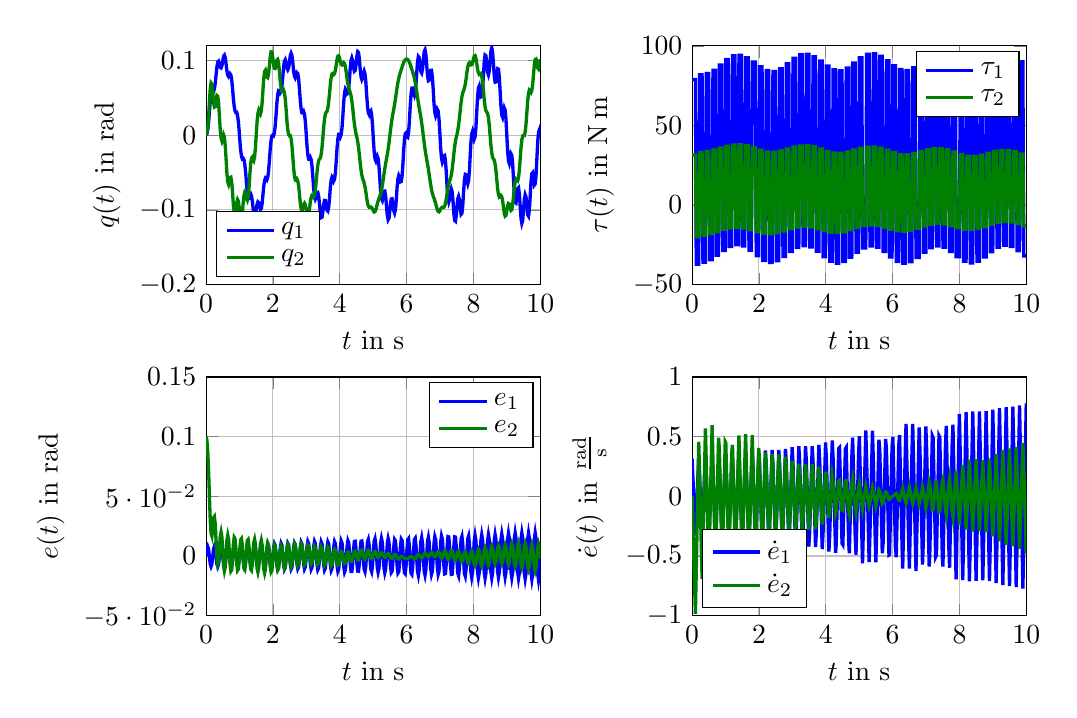
\begin{tikzpicture}

\begin{axis}[%
width=0.35\textwidth,
height=0.25\textwidth,
scale only axis,
xmin=0,
xmax=10,
xlabel={$t$ in $\mathrm{s}$},
xmajorgrids,
ymin=-0.2,
ymax=0.12,
ylabel={$q(t)$ in $\mathrm{rad}$},
ymajorgrids,
name=plot1,
legend style={at={(0.03,0.03)},anchor=south west,draw=black,fill=white,legend cell align=left}
]
\addplot [
color=blue,
solid,
line width=1.2pt
]
table[row sep=crcr]{
0 0\\
0.024133773460009 0.00182979361784962\\
0.049133773460009 0.00758473749279645\\
0.0741337734600091 0.0172718865204955\\
0.0991337734600091 0.0309098312653132\\
0.124 0.0445656401338809\\
0.149 0.0538890300545039\\
0.174 0.058746286554424\\
0.199 0.0591297532222548\\
0.224 0.0588624102204437\\
0.249 0.0623862532375738\\
0.274 0.0697083073666078\\
0.299 0.0808386716918216\\
0.324 0.0918049605469498\\
0.349 0.0979329493128981\\
0.374 0.0992084185190537\\
0.399 0.0956502954872333\\
0.424 0.0911929864602152\\
0.449 0.0904060226295566\\
0.474 0.0932983038287358\\
0.499 0.0998732088684403\\
0.523999999999997 0.10617128907491\\
0.548999999999995 0.107566763239672\\
0.573999999999992 0.104055101668648\\
0.598999999999989 0.0956313600963136\\
0.623999999999986 0.0862738443410808\\
0.648999999999984 0.0806640023330815\\
0.673999999999981 0.0788297325226902\\
0.698999999999978 0.0807791528526975\\
0.716668559556474 0.0825293620628186\\
0.741668559556471 0.0809250867638176\\
0.766668559556469 0.0745226258162933\\
0.791668559556466 0.0632897336164357\\
0.816499999999998 0.0492608466499462\\
0.841499999999995 0.0387847663593493\\
0.866499999999993 0.0325217255730468\\
0.89149999999999 0.0304932794496859\\
0.916499999999987 0.0307560541035293\\
0.941499999999984 0.0268716460174837\\
0.966499999999982 0.0183249829210145\\
0.991499999999979 0.00507978251457341\\
1.00916771252353 -0.00651255488165097\\
1.03416771252353 -0.0196344430064958\\
1.05916771252352 -0.0279507916509894\\
1.08416771252352 -0.0314354286293736\\
1.109 -0.0307241813382692\\
1.134 -0.0326088644375047\\
1.15899999999999 -0.0389678077899173\\
1.18399999999999 -0.0498042548810179\\
1.20899999999999 -0.0645188038259516\\
1.23399999999999 -0.0760111081939932\\
1.25899999999998 -0.0822554977971162\\
1.28399999999998 -0.0832408459563497\\
1.30899999999998 -0.0795949315278691\\
1.33399999999997 -0.0782691278092187\\
1.35899999999997 -0.0811835063157192\\
1.38399999999997 -0.0883258437445898\\
1.40175241581824 -0.0959414827834113\\
1.42675241581824 -0.104849114887697\\
1.45175241581823 -0.108386479610544\\
1.47675241581823 -0.106548027520179\\
1.5015 -0.0994479218766042\\
1.5265 -0.0922352715668996\\
1.55149999999999 -0.0891605797023249\\
1.57649999999999 -0.0902272403425078\\
1.60149999999999 -0.095418008901098\\
1.62649999999999 -0.0994749111148397\\
1.65149999999998 -0.0982279870407602\\
1.67649999999998 -0.0916704196360128\\
1.70149999999998 -0.0797949334556556\\
1.72649999999998 -0.067979424954648\\
1.75149999999997 -0.0605545468252765\\
1.77649999999997 -0.0575631192784506\\
1.80000000000099 -0.0588076584980955\\
1.81925241581824 -0.0598808829839391\\
1.84425241581824 -0.0566398531027218\\
1.86925241581823 -0.0481575170987862\\
1.89425241581823 -0.0344063737177019\\
1.919 -0.0185228777468491\\
1.944 -0.00716307763069127\\
1.96899999999999 -0.000855979412466308\\
1.99399999999999 0.000371922059791658\\
2.019 -0.000507070764460296\\
2.044 0.00349871639093979\\
2.06900000000001 0.0126839039536734\\
2.09400000000002 0.0270689896951099\\
2.11900000000001 0.0435492555675883\\
2.14400000000001 0.0546764165925925\\
2.16900000000002 0.0600934649167686\\
2.19400000000003 0.059798648393256\\
2.21900000000001 0.0569185781399154\\
2.24400000000001 0.0587729118837723\\
2.26900000000002 0.0656649205598546\\
2.29400000000003 0.0776032641626122\\
2.31900000000001 0.0913911729030022\\
2.34400000000002 0.099426620024276\\
2.36900000000002 0.101382413767173\\
2.39400000000003 0.0972740091877037\\
2.41900000000001 0.0902810335073064\\
2.44400000000002 0.087862413180679\\
2.46900000000002 0.0903308742390451\\
2.49400000000003 0.09769033725614\\
2.51900000000001 0.106764315266549\\
2.54400000000001 0.110040455481881\\
2.56900000000002 0.107205826846364\\
2.59400000000003 0.0982578378832037\\
2.61900000000001 0.0863772156919999\\
2.64400000000001 0.0791217110307828\\
2.66900000000002 0.0768252838078517\\
2.69400000000003 0.0794978621620626\\
2.71900000000001 0.083978647842024\\
2.74400000000001 0.0828025425013761\\
2.76900000000002 0.0756473972175033\\
2.79400000000003 0.062479168021439\\
2.81900000000001 0.0465344868066539\\
2.84400000000002 0.0356043023793449\\
2.86900000000002 0.0300518832036945\\
2.89400000000003 0.0298944906362969\\
2.91900000000001 0.0318919785736387\\
2.94400000000002 0.0283974922188854\\
2.96900000000002 0.0190799728501566\\
2.99400000000003 0.00390051929607333\\
3.01900000000001 -0.0137810776350727\\
3.04400000000001 -0.0258709043900018\\
3.06900000000002 -0.031988729580914\\
3.09400000000003 -0.0321203045833644\\
3.11900000000001 -0.0296331203354346\\
3.14400000000001 -0.032456055424483\\
3.16900000000002 -0.0409158193121953\\
3.19400000000003 -0.0550276189832474\\
3.21900000000001 -0.0713346802225462\\
3.24400000000001 -0.0815843961505153\\
3.26900000000002 -0.0854034966084029\\
3.29400000000003 -0.0827876040987853\\
3.31900000000001 -0.0771794239927508\\
3.34400000000002 -0.0766778734980045\\
3.36900000000002 -0.081606490189433\\
3.39400000000003 -0.0919593227429116\\
3.41900000000001 -0.104272813893482\\
3.44400000000002 -0.110352760897971\\
3.46900000000002 -0.10984385458018\\
3.49400000000003 -0.102742393215035\\
3.51900000000001 -0.0924998122085549\\
3.54400000000001 -0.0872780955504722\\
3.56900000000002 -0.0874224904577299\\
3.59400000000003 -0.0929329041713504\\
3.61900000000001 -0.100368468033534\\
3.64400000000001 -0.101610813361015\\
3.66900000000002 -0.0963119604438296\\
3.69400000000003 -0.0844559991252377\\
3.71900000000001 -0.0695317788917765\\
3.74400000000001 -0.0598659496054476\\
3.76900000000002 -0.0558492840170648\\
3.79400000000003 -0.0575032716876013\\
3.81900000000001 -0.0613245650063439\\
3.84400000000002 -0.0590375599574566\\
3.86900000000002 -0.0502867471723731\\
3.89400000000003 -0.0350476856853917\\
3.91900000000001 -0.0169482644229992\\
3.94400000000002 -0.00468350880321344\\
3.96900000000002 0.00132194466739227\\
3.99400000000003 0.00104234347140509\\
4.01899999999999 -0.00186063147311404\\
4.04399999999998 0.00125153748622161\\
4.06899999999996 0.0107464313454042\\
4.09399999999995 0.0266443904208246\\
4.11899999999993 0.0451426458643007\\
4.14399999999992 0.0571568388696426\\
4.16899999999991 0.0622667008654517\\
4.19399999999989 0.0604674651781013\\
4.21899999999988 0.0555698682509059\\
4.24399999999986 0.0565324726453153\\
4.26899999999985 0.0637309275838542\\
4.29399999999984 0.0771757806379732\\
4.3122534322576 0.0893233981977524\\
4.33725343225759 0.100205356486827\\
4.36225343225758 0.103810225023896\\
4.38725343225756 0.10014606833028\\
4.41199999999999 0.0909133602300246\\
4.43699999999998 0.085893851962544\\
4.46199999999997 0.0869600310005569\\
4.48699999999995 0.0941148613273358\\
4.51199999999994 0.105819622505851\\
4.53699999999992 0.112024926811566\\
4.56199999999991 0.110924170611061\\
4.5869999999999 0.102517221275151\\
4.61199999999988 0.0883397032679383\\
4.63699999999987 0.0784735029944196\\
4.66199999999986 0.0747475676127519\\
4.68699999999984 0.0771708746670303\\
4.70525343225761 0.0825326601233734\\
4.73025343225759 0.0861556153067941\\
4.75525343225758 0.0826328420105979\\
4.78025343225757 0.07194685544505\\
4.805 0.0545442349323041\\
4.82999999999998 0.0390958414065892\\
4.85499999999997 0.0301681380192717\\
4.87999999999996 0.0277842784228923\\
4.90499999999994 0.0316818048181162\\
4.92999999999993 0.0329384923245608\\
4.95499999999991 0.0272296916167862\\
4.9799999999999 0.014533001102588\\
5.00499999999989 -0.00491894846606293\\
5.02999999999987 -0.0218292529523161\\
5.05499999999986 -0.0316381401746668\\
5.07999999999985 -0.034318681020864\\
5.10000040549141 -0.0313266526649389\\
5.1232534322576 -0.028139724365204\\
5.14825343225758 -0.0312709196932877\\
5.17325343225757 -0.0411975204134359\\
5.19825343225756 -0.0579387345814266\\
5.22299999999999 -0.0751528110178028\\
5.24799999999997 -0.0850376207046291\\
5.27299999999996 -0.0873196206796002\\
5.29799999999995 -0.0819951721312157\\
5.32299999999993 -0.0750995687716686\\
5.34799999999992 -0.07479045227233\\
5.3729999999999 -0.0811008567235061\\
5.39799999999989 -0.0940265108085932\\
5.42299999999988 -0.107476234728314\\
5.44799999999986 -0.113183942553264\\
5.47299999999985 -0.111092654221658\\
5.49799999999984 -0.101198696958017\\
5.5162534322576 -0.092087192058495\\
5.54125343225759 -0.0852435635161687\\
5.56625343225757 -0.0849877762539154\\
5.59125343225756 -0.0913181389330759\\
5.61599999999999 -0.101127010548701\\
5.64099999999998 -0.104199448518119\\
5.66599999999996 -0.0995030900541435\\
5.69099999999995 -0.087025433306453\\
5.71599999999994 -0.0697404403457347\\
5.74099999999992 -0.0583407239465804\\
5.76599999999991 -0.0538092754016084\\
5.79099999999989 -0.0561660138695393\\
5.81599999999988 -0.0624296530563998\\
5.84099999999987 -0.0619639631737489\\
5.86599999999985 -0.0538201850170945\\
5.89099999999984 -0.0379784155964327\\
5.90925343225761 -0.0225645729544957\\
5.93425343225759 -0.00650519427772425\\
5.95925343225758 0.00211064757599192\\
5.98425343225756 0.00324757134768194\\
6.009 -0.00202344653369372\\
6.03399999999998 -0.00282972770059658\\
6.05899999999997 0.00393770077566019\\
6.08399999999995 0.0182930447833996\\
6.10899999999994 0.039251379426002\\
6.13399999999993 0.0553762175487136\\
6.15899999999991 0.0634195249504963\\
6.1839999999999 0.0633639324321941\\
6.20899999999988 0.0562219140401029\\
6.23399999999987 0.0533309346382254\\
6.25899999999986 0.0578632321710992\\
6.28399999999984 0.0698266892356321\\
6.30225478751033 0.0832030853395741\\
6.32725478751031 0.0986702640106736\\
6.3522547875103 0.10567207956591\\
6.37725478751028 0.104210685457132\\
6.402 0.0944902593751253\\
6.42699999999999 0.0853387393381422\\
6.45199999999997 0.0834642858300118\\
6.47699999999996 0.0888670062182829\\
6.50199999999994 0.101503676062791\\
6.52699999999993 0.112321061605917\\
6.55199999999992 0.114643335889487\\
6.5769999999999 0.108475454420231\\
6.60199999999989 0.0938581041619606\\
6.62699999999987 0.0798544917406679\\
6.65199999999986 0.0731656791622386\\
6.67699999999985 0.0737978218253719\\
6.70000000002574 0.0808492639131191\\
6.7202534322576 0.0870599822350992\\
6.74525343225759 0.0872053924054415\\
6.77025343225757 0.0790350013256739\\
6.79525343225756 0.0625161510307559\\
6.81999999999999 0.0430316640938162\\
6.84499999999998 0.0306778494387122\\
6.86999999999996 0.026008636636149\\
6.89499999999995 0.0290355997331617\\
6.91999999999993 0.0347017997039092\\
6.94499999999992 0.0325805657277685\\
6.96999999999991 0.0223442437671891\\
6.99499999999989 0.00395427665219011\\
7.01999999999988 -0.017388313099171\\
7.04499999999986 -0.0308359769817287\\
7.06999999999985 -0.0360264746282659\\
7.09499999999984 -0.0329466767927553\\
7.1132534322576 -0.0277547749632884\\
7.13825343225759 -0.0270680004906553\\
7.16325343225758 -0.0343176650861277\\
7.18825343225756 -0.0495179032375928\\
7.21299999999999 -0.0701633107051777\\
7.23799999999998 -0.0842040377069576\\
7.26299999999997 -0.0894902073021296\\
7.28799999999995 -0.0860088977010369\\
7.31299999999994 -0.0760066630007704\\
7.33799999999992 -0.0719077967911526\\
7.36299999999991 -0.0756102190181791\\
7.3879999999999 -0.0871089697609381\\
7.41299999999988 -0.104135829186085\\
7.43799999999987 -0.114117371778841\\
7.46299999999985 -0.115105474867385\\
7.48799999999984 -0.107093273312957\\
7.50625343225761 -0.0960841703190418\\
7.53125343225759 -0.0851015476965286\\
7.55625343225758 -0.0819182548285704\\
7.58125343225757 -0.0865329659098965\\
7.606 -0.0982899692330563\\
7.63099999999998 -0.105995314703288\\
7.65599999999997 -0.104717792753063\\
7.68099999999996 -0.0944489055568756\\
7.70599999999994 -0.0756653772433777\\
7.73099999999993 -0.0599964798106631\\
7.75599999999991 -0.0523974785975382\\
7.7809999999999 -0.0528907838740632\\
7.80599999999989 -0.060991765058366\\
7.83099999999987 -0.0651160966719383\\
7.85599999999986 -0.0603631532728596\\
7.88099999999984 -0.0467211738255517\\
7.90001013729011 -0.0303821697210311\\
7.9242534322576 -0.0102889062507173\\
7.94925343225758 0.00194711529066477\\
7.97425343225757 0.00552653901625234\\
7.99925343225756 0.000433327128986538\\
8.02400000000003 -0.00511685416229631\\
8.04900000000006 -0.00202434703171335\\
8.07400000000009 0.0098268433058631\\
8.09900000000012 0.0304623352265501\\
8.12400000000003 0.0516050057941338\\
8.14900000000006 0.0635211510499731\\
8.17400000000009 0.0661692880992579\\
8.19900000000012 0.0595455686213528\\
8.22400000000003 0.051890555743058\\
8.24900000000006 0.0528165776790727\\
8.27400000000009 0.0623409646274615\\
8.29900000000012 0.0804836081304031\\
8.32400000000003 0.0988462775570505\\
8.34900000000006 0.107585722903632\\
8.37400000000009 0.106688113207332\\
8.39900000000012 0.0961597349858319\\
8.42400000000003 0.084338549971898\\
8.44900000000006 0.0809543863183234\\
8.47400000000009 0.0860204314970896\\
8.49900000000012 0.0995452670407845\\
8.52400000000003 0.113177178539227\\
8.54900000000006 0.117157211957091\\
8.57400000000009 0.111479210469278\\
8.59900000000012 0.096134349035603\\
8.62400000000003 0.079473101075047\\
8.64900000000006 0.0712729431109834\\
8.67400000000009 0.071551633819338\\
8.69900000000012 0.080311800274684\\
8.72400000000003 0.0892835443951091\\
8.74900000000006 0.0888133579187181\\
8.77400000000009 0.0788811512647509\\
8.79900000000012 0.0594509895689146\\
8.82400000000003 0.0389241191561571\\
8.84900000000006 0.0271811672009081\\
8.87400000000009 0.0242555189117117\\
8.89900000000012 0.0301528854096659\\
8.92400000000003 0.0365533109783607\\
8.94900000000006 0.0337449982433747\\
8.97400000000009 0.0216994148520868\\
8.99900000000012 0.000373600496608451\\
9.02400000000003 -0.0216864203554967\\
9.04900000000006 -0.0344146067958934\\
9.07400000000009 -0.037764867686602\\
9.09900000000012 -0.0317293722846631\\
9.12400000000003 -0.0248131778526312\\
9.14900000000006 -0.0269390301745431\\
9.17400000000009 -0.0381268997398563\\
9.19900000000012 -0.0584004485596524\\
9.22400000000003 -0.0790500271698876\\
9.24900000000006 -0.0898418801356408\\
9.27400000000009 -0.0907323396768726\\
9.29900000000012 -0.0817175053048106\\
9.32400000000003 -0.0714993553727342\\
9.34900000000006 -0.0702271024571103\\
9.37400000000009 -0.0779098143580439\\
9.39900000000012 -0.0945463629202039\\
9.42400000000003 -0.111337176316093\\
9.44900000000006 -0.117984698295083\\
9.47400000000009 -0.114458107239833\\
9.49900000000012 -0.100755430229549\\
9.52400000000003 -0.0857083042660482\\
9.54900000000006 -0.079634164893042\\
9.57400000000009 -0.082548449801405\\
9.59900000000012 -0.0944430058537053\\
9.62400000000003 -0.106485686387359\\
9.64900000000006 -0.108368052613568\\
9.67400000000009 -0.100068932707475\\
9.69900000000012 -0.0815788502566118\\
9.72400000000003 -0.0618403497608101\\
9.74900000000006 -0.0513388129862818\\
9.77400000000009 -0.0501140180727161\\
9.79900000000012 -0.0581701758843859\\
9.82400000000003 -0.0665897546288559\\
9.84900000000006 -0.0649691044255354\\
9.87400000000009 -0.0532892226029515\\
9.89900000000012 -0.0315288182650981\\
9.92400000000003 -0.00880778613452255\\
9.94900000000006 0.0041491102898621\\
9.97400000000009 0.00728593089981392\\
9.99900000000012 0.000589835219059841\\
};
\addlegendentry{$q_1$};

\addplot [
color=green!50!black,
solid,
line width=1.2pt
]
table[row sep=crcr]{
0 0\\
0.024133773460009 0.00262475917474352\\
0.049133773460009 0.0108783319183001\\
0.0741337734600091 0.0247554207108192\\
0.0991337734600091 0.0442216817698687\\
0.124 0.0619891380945962\\
0.149 0.0701212058402822\\
0.174 0.0685875765072934\\
0.199 0.057409451214201\\
0.224 0.0441970602978374\\
0.249 0.0378875951024268\\
0.274 0.0384896982102607\\
0.299 0.0459861930053831\\
0.324 0.0533443390933039\\
0.349 0.0524160092393386\\
0.374 0.0432115000410569\\
0.399 0.0256888252839716\\
0.424 0.00710178986451996\\
0.449 -0.00401740443332\\
0.474 -0.00766721248434454\\
0.499 -0.00385459814279297\\
0.523999999999997 0.000468052432104726\\
0.548999999999995 -0.00282406061642122\\
0.573999999999992 -0.013748922412568\\
0.598999999999989 -0.0323048506436269\\
0.623999999999986 -0.0513116631631075\\
0.648999999999984 -0.062440708405062\\
0.673999999999981 -0.0657240289892592\\
0.698999999999978 -0.0611784713175981\\
0.716668559556474 -0.0565556108452348\\
0.741668559556471 -0.0560534077953665\\
0.766668559556469 -0.0626369331775425\\
0.791668559556466 -0.0762407668024069\\
0.816499999999998 -0.0933528594715826\\
0.841499999999995 -0.10354493704679\\
0.866499999999993 -0.105933385625165\\
0.89149999999999 -0.100561963435704\\
0.916499999999987 -0.0905267131941935\\
0.941499999999984 -0.0861606089839613\\
0.966499999999982 -0.0882805298619551\\
0.991499999999979 -0.0968032382173053\\
1.00916771252353 -0.105675124626916\\
1.03416771252353 -0.112935645909673\\
1.05916771252352 -0.112763988605096\\
1.08416771252352 -0.105214660298845\\
1.109 -0.091283402113662\\
1.134 -0.0806251578755045\\
1.15899999999999 -0.0761238151082694\\
1.18399999999999 -0.0777656662809218\\
1.20899999999999 -0.0846201020991828\\
1.23399999999999 -0.0870527195521982\\
1.25899999999998 -0.0824318153953472\\
1.28399999999998 -0.0707857309321152\\
1.30899999999998 -0.0529702625296944\\
1.33399999999997 -0.0387223684838645\\
1.35899999999997 -0.0308351201728034\\
1.38399999999997 -0.029334580712784\\
1.40175241581824 -0.0321106452002568\\
1.42675241581824 -0.0339726980335296\\
1.45175241581823 -0.0289960659376687\\
1.47675241581823 -0.017195129721654\\
1.5015 0.00116643587027787\\
1.5265 0.0188559898144359\\
1.55149999999999 0.0296818213091194\\
1.57649999999999 0.033644148016939\\
1.60149999999999 0.0307646552004463\\
1.62649999999999 0.028477711011684\\
1.65149999999998 0.0326977418275895\\
1.67649999999998 0.043409128639846\\
1.70149999999998 0.0605311015721501\\
1.72649999999998 0.0764700005887654\\
1.75149999999997 0.0853220107067762\\
1.77649999999997 0.0871754803703845\\
1.80000000000099 0.0825665640000821\\
1.81925241581824 0.0779870307851626\\
1.84425241581824 0.0771878223348536\\
1.86925241581823 0.0821928128920014\\
1.89425241581823 0.0929440137520016\\
1.919 0.105553120575356\\
1.944 0.111930496952797\\
1.96899999999999 0.111733854844546\\
1.99399999999999 0.105027089777376\\
2.019 0.0951241785734643\\
2.044 0.0899079871347788\\
2.06900000000001 0.0897055090642921\\
2.09400000000002 0.0944726069809661\\
2.11900000000001 0.100987824044671\\
2.14400000000001 0.101878401505658\\
2.16900000000002 0.0969401346220821\\
2.19400000000003 0.0861860431528856\\
2.21900000000001 0.0725974834980625\\
2.24400000000001 0.063352521281833\\
2.26900000000002 0.058755874939604\\
2.29400000000003 0.0587865463795761\\
2.31900000000001 0.0605628785384346\\
2.34400000000002 0.0573798669763135\\
2.36900000000002 0.0489780518529617\\
2.39400000000003 0.0353247513355435\\
2.41900000000001 0.0192999647276373\\
2.44400000000002 0.00783226395100555\\
2.46900000000002 0.00120971834724316\\
2.49400000000003 -0.000578120903287895\\
2.51900000000001 -0.000318954272802168\\
2.54400000000001 -0.00458896534901025\\
2.56900000000002 -0.013674846662581\\
2.59400000000003 -0.0275783649631851\\
2.61900000000001 -0.0433842296174501\\
2.64400000000001 -0.0542738048149938\\
2.66900000000002 -0.0599930782007848\\
2.69400000000003 -0.0605625896787232\\
2.71900000000001 -0.0587318919860521\\
2.74400000000001 -0.0610084794470291\\
2.76900000000002 -0.0676531596201701\\
2.79400000000003 -0.0785954298080916\\
2.81900000000001 -0.0909999338993465\\
2.84400000000002 -0.0984683056061075\\
2.86900000000002 -0.100799807098489\\
2.89400000000003 -0.0980302902553033\\
2.91900000000001 -0.0927353000636685\\
2.94400000000002 -0.0910139380350727\\
2.96900000000002 -0.0931015878615325\\
2.99400000000003 -0.0989064523254019\\
3.01900000000001 -0.105857628461879\\
3.04400000000001 -0.108235107406611\\
3.06900000000002 -0.105877204673896\\
3.09400000000003 -0.0988186377705739\\
3.11900000000001 -0.0893981909244718\\
3.14400000000001 -0.0831818242307349\\
3.16900000000002 -0.0804168270708696\\
3.19400000000003 -0.0810597186631091\\
3.21900000000001 -0.0828068643759627\\
3.24400000000001 -0.0804270752124577\\
3.26900000000002 -0.0737544065159518\\
3.29400000000003 -0.0628076428966721\\
3.31900000000001 -0.0498269989820203\\
3.34400000000002 -0.0401561616956315\\
3.36900000000002 -0.0340623415163674\\
3.39400000000003 -0.0315552749785585\\
3.41900000000001 -0.0304310651968447\\
3.44400000000002 -0.0255176582143742\\
3.46900000000002 -0.0166183704583393\\
3.49400000000003 -0.00374933124783546\\
3.51900000000001 0.0107815046104805\\
3.54400000000001 0.0215538503383471\\
3.56900000000002 0.0283331279486699\\
3.59400000000003 0.0311154655743655\\
3.61900000000001 0.0320923625676683\\
3.64400000000001 0.0364711379485494\\
3.66900000000002 0.0444609107006905\\
3.69400000000003 0.056024128505034\\
3.71900000000001 0.0688517797799749\\
3.74400000000001 0.0776749993548652\\
3.76900000000002 0.0823540390867706\\
3.79400000000003 0.0829341672290797\\
3.81900000000001 0.0814487416015855\\
3.84400000000002 0.0827101018160344\\
3.86900000000002 0.0869075686869306\\
3.89400000000003 0.0939871082423269\\
3.91900000000001 0.101917520670677\\
3.94400000000002 0.10617314286856\\
3.96900000000002 0.106698707001326\\
3.99400000000003 0.103557206179257\\
4.01899999999999 0.0984322670737518\\
4.04399999999998 0.0953239743494359\\
4.06899999999996 0.0943896915831798\\
4.09399999999995 0.0955821978059894\\
4.11899999999993 0.097324157539058\\
4.14399999999992 0.0961172991219182\\
4.16899999999991 0.0919129146002784\\
4.19399999999989 0.0847308889583748\\
4.21899999999988 0.0759260043771172\\
4.24399999999986 0.068791942723238\\
4.26899999999985 0.0634642123964113\\
4.29399999999984 0.0599154456378251\\
4.3122534322576 0.0579243480670048\\
4.33725343225759 0.0532819914533058\\
4.36225343225758 0.0462638138965969\\
4.38725343225756 0.0368560398097368\\
4.41199999999999 0.0256605782499979\\
4.43699999999998 0.015756028096479\\
4.46199999999997 0.00785151215366708\\
4.48699999999995 0.00193638286392517\\
4.51199999999994 -0.00245502174312188\\
4.53699999999992 -0.00827814970966603\\
4.56199999999991 -0.0160787400226824\\
4.5869999999999 -0.0258620089023258\\
4.61199999999988 -0.0371053994655881\\
4.63699999999987 -0.0465482419367596\\
4.66199999999986 -0.0536285493870184\\
4.68699999999984 -0.0583659761290792\\
4.70525343225761 -0.0604344309626933\\
4.73025343225759 -0.0639105842020939\\
4.75525343225758 -0.0689777898276002\\
4.78025343225757 -0.0756007412139067\\
4.805 -0.0835138238050592\\
4.82999999999998 -0.0902710268353605\\
4.85499999999997 -0.0946258407718822\\
4.87999999999996 -0.0966275454512007\\
4.90499999999994 -0.0963600016222298\\
4.92999999999993 -0.0960721200125089\\
4.95499999999991 -0.0968574629224038\\
4.9799999999999 -0.0986613844122659\\
5.00499999999989 -0.101302585064178\\
5.02999999999987 -0.102783194428522\\
5.05499999999986 -0.102254841005748\\
5.07999999999985 -0.0997786900263656\\
5.10000040549141 -0.0964069268344067\\
5.1232534322576 -0.0920391495297962\\
5.14825343225758 -0.087976573447607\\
5.17325343225757 -0.0845638509603455\\
5.19825343225756 -0.0817444653309767\\
5.22299999999999 -0.0785914874586251\\
5.24799999999997 -0.0739164793632694\\
5.27299999999996 -0.0677953997895871\\
5.29799999999995 -0.0602451621121256\\
5.32299999999993 -0.0521313117943097\\
5.34799999999992 -0.044669091875353\\
5.3729999999999 -0.0378941430193498\\
5.39799999999989 -0.0318105215823725\\
5.42299999999988 -0.0256591705841076\\
5.44799999999986 -0.018443273203075\\
5.47299999999985 -0.0101839207981368\\
5.49799999999984 -0.000897181508333373\\
5.5162534322576 0.00609703300767657\\
5.54125343225759 0.0148060626723901\\
5.56625343225757 0.0224927308358701\\
5.59125343225756 0.0291492090756241\\
5.61599999999999 0.0350524353651047\\
5.64099999999998 0.0415472007258167\\
5.66599999999996 0.048670769455292\\
5.69099999999995 0.0563929123956658\\
5.71599999999994 0.0642875458525918\\
5.74099999999992 0.0710480827691382\\
5.76599999999991 0.0766337512839519\\
5.79099999999989 0.0810867525859742\\
5.81599999999988 0.0846346568271193\\
5.84099999999987 0.0880963452971072\\
5.86599999999985 0.0915360843357766\\
5.89099999999984 0.0949073038591005\\
5.90925343225761 0.097219420775082\\
5.93425343225759 0.0996264143983126\\
5.95925343225758 0.101202040641492\\
5.98425343225756 0.102034372655575\\
6.009 0.102141168891949\\
6.03399999999998 0.101508874206442\\
6.05899999999997 0.100131345616946\\
6.08399999999995 0.0979723998623273\\
6.10899999999994 0.0949995759706747\\
6.13399999999993 0.0916783249272521\\
6.15899999999991 0.0882543938548115\\
6.1839999999999 0.0847811671344506\\
6.20899999999988 0.0811766902239859\\
6.23399999999987 0.0766630458099734\\
6.25899999999986 0.0710321654547243\\
6.28399999999984 0.0642597459442245\\
6.30225478751033 0.0585720555930192\\
6.32725478751031 0.0507457152252726\\
6.3522547875103 0.0434710820964199\\
6.37725478751028 0.0367528601992746\\
6.402 0.0306210611205019\\
6.42699999999999 0.0240953617788908\\
6.45199999999997 0.0166338199947488\\
6.47699999999996 0.00822992289341715\\
6.50199999999994 -0.00112771676957898\\
6.52699999999993 -0.0103361299749877\\
6.55199999999992 -0.0185896322204156\\
6.5769999999999 -0.02590272904819\\
6.60199999999989 -0.0322659130676824\\
6.62699999999987 -0.0385151393429942\\
6.65199999999986 -0.0453007319523426\\
6.67699999999985 -0.0526394443892922\\
6.70000000002574 -0.0598857226687351\\
6.7202534322576 -0.0660454075065714\\
6.74525343225759 -0.0724825554290131\\
6.77025343225757 -0.0776225855639438\\
6.79525343225756 -0.0813932005884821\\
6.81999999999999 -0.0842718094818574\\
6.84499999999998 -0.0875727406425023\\
6.86999999999996 -0.0913584882376355\\
6.89499999999995 -0.0956526460094973\\
6.91999999999993 -0.0997211509333659\\
6.94499999999992 -0.102071155401993\\
6.96999999999991 -0.102630389765273\\
6.99499999999989 -0.101300302005018\\
7.01999999999988 -0.0988400565336325\\
7.04499999999986 -0.097127316439299\\
7.06999999999985 -0.0963005199657738\\
7.09499999999984 -0.0963914601107697\\
7.1132534322576 -0.0965898168256376\\
7.13825343225759 -0.0950247368490136\\
7.16325343225758 -0.0912429925906288\\
7.18825343225756 -0.0852006653610663\\
7.21299999999999 -0.0774148355681886\\
7.23799999999998 -0.0705068823569449\\
7.26299999999997 -0.0650597467622853\\
7.28799999999995 -0.0611094055689364\\
7.31299999999994 -0.0581329162325046\\
7.33799999999992 -0.0532716420225633\\
7.36299999999991 -0.0461161049304113\\
7.3879999999999 -0.0366737041200183\\
7.41299999999988 -0.0255076191726014\\
7.43799999999987 -0.0157873071319438\\
7.46299999999985 -0.00803818149645485\\
7.48799999999984 -0.00228069234608047\\
7.50625343225761 0.000786707809592696\\
7.53125343225759 0.00611533504590521\\
7.55625343225758 0.0134810970223837\\
7.58125343225757 0.0228759956332308\\
7.606 0.034025479572611\\
7.63099999999998 0.0441271150310477\\
7.65599999999997 0.0517944902765978\\
7.68099999999996 0.0570092588689346\\
7.70599999999994 0.0598545614219807\\
7.73099999999993 0.0632489777114189\\
7.75599999999991 0.0685080991239449\\
7.7809999999999 0.0756820953028254\\
7.80599999999989 0.0846316077300167\\
7.83099999999987 0.091950426221308\\
7.85599999999986 0.0962116938562446\\
7.88099999999984 0.097389057708471\\
7.90001013729011 0.0961773427282232\\
7.9242534322576 0.0944078024693226\\
7.94925343225758 0.0946943755922964\\
7.97425343225757 0.0972343159059673\\
7.99925343225756 0.102066973498364\\
8.02400000000003 0.106312546120451\\
8.04900000000006 0.106875348387911\\
8.07400000000009 0.103673397345454\\
8.09900000000012 0.096637476637869\\
8.12400000000003 0.0887682786986169\\
8.14900000000006 0.0837507236503995\\
8.17400000000009 0.0816743733272163\\
8.19900000000012 0.0825532633914967\\
8.22400000000003 0.0831086610359556\\
8.24900000000006 0.0795517598650844\\
8.27400000000009 0.0718651453796877\\
8.29900000000012 0.05999454123486\\
8.32400000000003 0.0474631471879555\\
8.34900000000006 0.038481281937747\\
8.37400000000009 0.0330658578383608\\
8.39900000000012 0.0312005123972355\\
8.42400000000003 0.0294161722373598\\
8.44900000000006 0.0236919078528437\\
8.47400000000009 0.014018742679433\\
8.49900000000012 0.000374371856226121\\
8.52400000000003 -0.0135886808860959\\
8.54900000000006 -0.0236014775854762\\
8.57400000000009 -0.0296800742206843\\
8.59900000000012 -0.0318111023988511\\
8.62400000000003 -0.0334101195381801\\
8.64900000000006 -0.0385169433057197\\
8.67400000000009 -0.047150242776748\\
8.69900000000012 -0.0593129240641765\\
8.72400000000003 -0.071409777872371\\
8.74900000000006 -0.0792767272973961\\
8.77400000000009 -0.0829010635210711\\
8.79900000000012 -0.082198229928028\\
8.82400000000003 -0.0806359438405004\\
8.84900000000006 -0.0824319228230626\\
8.87400000000009 -0.0876412059930333\\
8.89900000000012 -0.0962724413287219\\
8.92400000000003 -0.104579932786628\\
8.94900000000006 -0.108225172712776\\
8.97400000000009 -0.1071685366962\\
8.99900000000012 -0.101294330801508\\
9.02400000000003 -0.0944400014456445\\
9.04900000000006 -0.0913107997085671\\
9.07400000000009 -0.0919945571232024\\
9.09900000000012 -0.0965089471214748\\
9.12400000000003 -0.100695414225558\\
9.14900000000006 -0.0997397622862056\\
9.17400000000009 -0.0936188893729249\\
9.19900000000012 -0.0822580486349426\\
9.22400000000003 -0.0700206690165146\\
9.24900000000006 -0.0621729779057402\\
9.27400000000009 -0.0587979511035651\\
9.29900000000012 -0.0599090402927024\\
9.32400000000003 -0.060956639026056\\
9.34900000000006 -0.0566725901555754\\
9.37400000000009 -0.0470648695437201\\
9.39900000000012 -0.0321270731013042\\
9.42400000000003 -0.0166094160408457\\
9.44900000000006 -0.00611315938931485\\
9.47400000000009 -0.00068491385968608\\
9.49900000000012 -0.000335518707432439\\
9.52400000000003 -0.000348361772691115\\
9.54900000000006 0.00478650844084403\\
9.57400000000009 0.0150716381783469\\
9.59900000000012 0.0304851338285682\\
9.62400000000003 0.0460843333198016\\
9.64900000000006 0.0561308258818144\\
9.67400000000009 0.0606077831176309\\
9.69900000000012 0.0594850774970631\\
9.72400000000003 0.0575850184881968\\
9.74900000000006 0.0606460132620133\\
9.77400000000009 0.0687345307404078\\
9.79900000000012 0.0818557387726574\\
9.82400000000003 0.0948257356239246\\
9.84900000000006 0.101645345207645\\
9.87400000000009 0.102303232766717\\
9.89900000000012 0.0967371631207262\\
9.92400000000003 0.0901286134581614\\
9.94900000000006 0.0887311185383848\\
9.97400000000009 0.0926644097749525\\
9.99900000000012 0.101960022967806\\
};
\addlegendentry{$q_2$};

\end{axis}

\begin{axis}[%
width=0.35\textwidth,
height=0.25\textwidth,
scale only axis,
xmin=0,
xmax=10,
xlabel={$t$ in $\mathrm{s}$},
xmajorgrids,
ymin=-0.05,
ymax=0.15,
ylabel={$e(t)$ in $\mathrm{rad}$},
ymajorgrids,
name=plot3,
at=(plot1.below south west),
anchor=above north west,
legend style={draw=black,fill=white,legend cell align=left}
]
\addplot [
color=blue,
solid,
line width=1.2pt
]
table[row sep=crcr]{
0 0\\
0.024133773460009 0.00574479303987424\\
0.049133773460009 0.00778986873465218\\
0.0741337734600091 0.00580794971671035\\
0.0991337734600091 -0.000267059883576892\\
0.124 -0.00658773058170074\\
0.149 -0.00877012161031939\\
0.174 -0.00676455229235306\\
0.199 -0.000605677819703748\\
0.224 0.00584318593650073\\
0.249 0.00810193215666236\\
0.274 0.0061278841622644\\
0.299 -0.000122029367181573\\
0.324 -0.0067055123674806\\
0.349 -0.00897536167506426\\
0.374 -0.00694114453204224\\
0.399 -0.000642193577156128\\
0.424 0.00597018683125224\\
0.449 0.00831317876992531\\
0.474 0.00636828897466715\\
0.499 0.000126297651745516\\
0.523999999999997 -0.00645539904884879\\
0.548999999999995 -0.00874927132864416\\
0.573999999999992 -0.00674525057043512\\
0.598999999999989 -0.000429097401744905\\
0.623999999999986 0.00623387634236661\\
0.648999999999984 0.00857883547929267\\
0.673999999999981 0.00659801064724243\\
0.698999999999978 0.000306805230543883\\
0.716668559556474 -0.00481514015574228\\
0.741668559556471 -0.00838805900690941\\
0.766668559556469 -0.00761000710668393\\
0.791668559556466 -0.00241406249917338\\
0.816499999999998 0.0052469620720071\\
0.841499999999995 0.00897711788013772\\
0.866499999999993 0.0081997662851993\\
0.89149999999999 0.00293675848874314\\
0.916499999999987 -0.00482357738542335\\
0.941499999999984 -0.00859661286209149\\
0.966499999999982 -0.00782006498480426\\
0.991499999999979 -0.00240974610986153\\
1.00916771252353 0.00363283121545074\\
1.03416771252353 0.00892094090049411\\
1.05916771252352 0.0094695634082707\\
1.08416771252352 0.00530041716768622\\
1.109 -0.00285385760098864\\
1.134 -0.00825604303612919\\
1.15899999999999 -0.00893202247455703\\
1.18399999999999 -0.00483517979240661\\
1.20899999999999 0.00347663502779427\\
1.23399999999999 0.00894255054032468\\
1.25899999999998 0.00957405124842968\\
1.28399999999998 0.00539461579965135\\
1.30899999999998 -0.00293613434142677\\
1.33399999999997 -0.00843794230722633\\
1.35899999999997 -0.00916499012758039\\
1.38399999999997 -0.00510705050106788\\
1.40175241581824 0.00066714780157652\\
1.42675241581824 0.00748507661402766\\
1.45175241581823 0.00953301971782648\\
1.47675241581823 0.00681461046076158\\
1.5015 -0.000550967794955434\\
1.5265 -0.00741838205977362\\
1.55149999999999 -0.00953343996665111\\
1.57649999999999 -0.00689866391841999\\
1.60149999999999 0.000459033545627582\\
1.62649999999999 0.00726831832495645\\
1.65149999999998 0.00934226112281722\\
1.67649999999998 0.00665357064779731\\
1.70149999999998 -0.00082888145784904\\
1.72649999999998 -0.00775428325506504\\
1.75149999999997 -0.00982213118551878\\
1.77649999999997 -0.00702263291087017\\
1.80000000000099 2.91332691004023e-05\\
1.81925241581824 0.00610005217133969\\
1.84425241581824 0.0096394392857729\\
1.86925241581823 0.00822729345789292\\
1.89425241581823 0.00179252335975707\\
1.919 -0.0066502771200012\\
1.944 -0.0103392282668378\\
1.96899999999999 -0.00886756997977596\\
1.99399999999999 -0.00225676603133567\\
2.019 0.00647255290347582\\
2.044 0.0102803126775251\\
2.06900000000001 0.00882371974804152\\
2.09400000000002 0.00203462698772328\\
2.11900000000001 -0.00702907937842769\\
2.14400000000001 -0.0109648399274951\\
2.16900000000002 -0.00945998418144906\\
2.19400000000003 -0.00255543583378888\\
2.21900000000001 0.00658144280296219\\
2.24400000000001 0.0105924186975115\\
2.26900000000002 0.00913805933048847\\
2.29400000000003 0.0021761797912508\\
2.31900000000001 -0.00712713168695781\\
2.34400000000002 -0.0111974973807784\\
2.36900000000002 -0.00973217157648051\\
2.39400000000003 -0.00276770166971994\\
2.41900000000001 0.0064986765255807\\
2.44400000000002 0.0105940202722424\\
2.46900000000002 0.00919526598158649\\
2.49400000000003 0.00229189798194109\\
2.51900000000001 -0.00694240873872842\\
2.54400000000001 -0.0109943129122163\\
2.56900000000002 -0.00954610063998325\\
2.59400000000003 -0.00258663272732357\\
2.61900000000001 0.00671562361969302\\
2.64400000000001 0.0108188141258523\\
2.66900000000002 0.00940841394787507\\
2.69400000000003 0.00249734877047698\\
2.71900000000001 -0.00672745147423885\\
2.74400000000001 -0.0107716400125886\\
2.76900000000002 -0.00928088307426292\\
2.79400000000003 -0.00218621385254439\\
2.81900000000001 0.00731318127601038\\
2.84400000000002 0.0114660908371843\\
2.86900000000002 0.00995103052002529\\
2.89400000000003 0.00279431232918804\\
2.91900000000001 -0.00671882370679102\\
2.94400000000002 -0.0108951863213623\\
2.96900000000002 -0.00935642345792399\\
2.99400000000003 -0.00201567532454236\\
3.01900000000001 0.00781559549605372\\
3.04400000000001 0.0120918753215334\\
3.06900000000002 0.0104811058791957\\
3.09400000000003 0.0030166879005278\\
3.11900000000001 -0.006887055853726\\
3.14400000000001 -0.0112555212406144\\
3.16900000000002 -0.0097176614231241\\
3.19400000000003 -0.00221559357621978\\
3.21900000000001 0.00783465927966853\\
3.24400000000001 0.0122190655692314\\
3.26900000000002 0.0106005167180598\\
3.29400000000003 0.00300816014492224\\
3.31900000000001 -0.0070846172232935\\
3.34400000000002 -0.011551249145493\\
3.36900000000002 -0.0100437520012597\\
3.39400000000003 -0.00254698477507213\\
3.41900000000001 0.0074931038605948\\
3.44400000000002 0.0118963274450498\\
3.46900000000002 0.0103177143595481\\
3.49400000000003 0.00276015797695374\\
3.51900000000001 -0.00732209431926618\\
3.54400000000001 -0.0117680470191923\\
3.56900000000002 -0.0102372357486511\\
3.59400000000003 -0.00273830098452982\\
3.61900000000001 0.00727562872184066\\
3.64400000000001 0.0116702882043796\\
3.66900000000002 0.0100782626881028\\
3.69400000000003 0.0024607881926981\\
3.71900000000001 -0.00771941747600867\\
3.74400000000001 -0.0121649528833398\\
3.76900000000002 -0.0105172301261756\\
3.79400000000003 -0.00278968248129329\\
3.81900000000001 0.00747689692367958\\
3.84400000000002 0.0119671667409274\\
3.86900000000002 0.0102838334486533\\
3.89400000000003 0.00235888271990675\\
3.91900000000001 -0.0082248904438485\\
3.94400000000002 -0.0128187970943096\\
3.96900000000002 -0.0110454940596249\\
3.99400000000003 -0.00292718744293607\\
4.01899999999999 0.00782611361212768\\
4.04399999999998 0.0125274915822346\\
4.06899999999996 0.0107611923562953\\
4.09399999999995 0.00245922626198689\\
4.11899999999993 -0.0086224696751613\\
4.14399999999992 -0.0134452622045719\\
4.16899999999991 -0.0116332201301638\\
4.19399999999989 -0.00322425261867002\\
4.21899999999988 0.00793015269194063\\
4.24399999999986 0.0128328579359346\\
4.26899999999985 0.0110720523064529\\
4.29399999999984 0.00260366331585296\\
4.3122534322576 -0.00621949723476742\\
4.33725343225759 -0.01299363130615\\
4.36225343225758 -0.0130283649121063\\
4.38725343225756 -0.00635377364299831\\
4.41199999999999 0.00528940692858346\\
4.43699999999998 0.0121539103747492\\
4.46199999999997 0.0123282294564232\\
4.48699999999995 0.00580175210691759\\
4.51199999999994 -0.00589067524179097\\
4.53699999999992 -0.0126997409073296\\
4.56199999999991 -0.0128151188667219\\
4.5869999999999 -0.00622917861928324\\
4.61199999999988 0.00553368249746183\\
4.63699999999987 0.0124064652412017\\
4.66199999999986 0.0125786778682623\\
4.68699999999984 0.00606325271706371\\
4.70525343225761 -0.00261202392843954\\
4.73025343225759 -0.0111971845019507\\
4.75525343225758 -0.0130987602479641\\
4.78025343225757 -0.00826582346112033\\
4.805 0.00295629027202429\\
4.82999999999998 0.0118083001684523\\
4.85499999999997 0.0138257789663284\\
4.87999999999996 0.00902817684558828\\
4.90499999999994 -0.0022777722948685\\
4.92999999999993 -0.0111241681848846\\
4.95499999999991 -0.0131395684230013\\
4.9799999999999 -0.00825394914962566\\
5.00499999999989 0.00334821673491637\\
5.02999999999987 0.0124184216205044\\
5.05499999999986 0.0144452301467695\\
5.07999999999985 0.00944969230442553\\
5.10000040549141 0.000424832073442759\\
5.1232534322576 -0.00962111223487474\\
5.14825343225758 -0.013638553645218\\
5.17325343225757 -0.0105837078264496\\
5.19825343225756 -0.000395000068734691\\
5.22299999999999 0.0106870621550466\\
5.24799999999997 0.0147726237247502\\
5.27299999999996 0.0116885826544613\\
5.29799999999995 0.0014643835601135\\
5.32299999999993 -0.00983447125465171\\
5.34799999999992 -0.0140231926090127\\
5.3729999999999 -0.011044827358632\\
5.39799999999989 -0.00088310369042538\\
5.42299999999988 0.0103878391464504\\
5.44799999999986 0.014515348132484\\
5.47299999999985 0.0114521856572026\\
5.49799999999984 0.00120067087240315\\
5.5162534322576 -0.00778247159062015\\
5.54125343225759 -0.0139177841647948\\
5.56625343225757 -0.0128538927759499\\
5.59125343225756 -0.00460062502046606\\
5.61599999999999 0.00769411630303894\\
5.64099999999998 0.013850952074812\\
5.66599999999996 0.0127960199376888\\
5.69099999999995 0.0044943674371441\\
5.71599999999994 -0.0081057898109803\\
5.74099999999992 -0.0143407226021266\\
5.76599999999991 -0.0132592822520851\\
5.79099999999989 -0.00487615492864718\\
5.81599999999988 0.00779021838294131\\
5.84099999999987 0.014064132909236\\
5.86599999999985 0.0129552775434175\\
5.89099999999984 0.00440037665712693\\
5.90925343225761 -0.0055596891150092\\
5.93425343225759 -0.0140031473383021\\
5.95925343225758 -0.0148766279927618\\
5.98425343225756 -0.0081924840508064\\
6.009 0.00485050321071956\\
6.03399999999998 0.0134908431281165\\
6.05899999999997 0.014491744080563\\
6.08399999999995 0.00779110584557571\\
6.10899999999994 -0.00567334048676194\\
6.13399999999993 -0.0145113100751\\
6.15899999999991 -0.0155196946860446\\
6.1839999999999 -0.00872449775879405\\
6.20899999999988 0.00482025475802856\\
6.23399999999987 0.0137376230154163\\
6.25899999999986 0.0148182143775601\\
6.28399999999984 0.00801954092103908\\
6.30225478751033 -0.00188705414251042\\
6.32725478751031 -0.0130382715079609\\
6.3522547875103 -0.0162520754668542\\
6.37725478751028 -0.011553973822172\\
6.402 0.000807674776596448\\
6.42699999999999 0.0120430104095696\\
6.45199999999997 0.0154008886437783\\
6.47699999999996 0.0108720563049485\\
6.50199999999994 -0.00150564997717739\\
6.52699999999993 -0.0126805930414559\\
6.55199999999992 -0.0159747414686958\\
6.5769999999999 -0.011387058838351\\
6.60199999999989 0.00105151033707998\\
6.62699999999987 0.0122911923414973\\
6.65199999999986 0.0156479657191359\\
6.67699999999985 0.0111362182009852\\
6.70000000002574 5.24355196219323e-05\\
6.7202534322576 -0.0100594328555041\\
6.74525343225759 -0.0154481926333928\\
6.77025343225757 -0.0129635581594564\\
6.79525343225756 -0.0025378168884731\\
6.81999999999999 0.0105510154040863\\
6.84499999999998 0.0161151319873518\\
6.86999999999996 0.0137061524273401\\
6.89499999999995 0.00335614208666869\\
6.91999999999993 -0.00983281098740352\\
6.94499999999992 -0.0153876556998028\\
6.96999999999991 -0.0129334124353085\\
6.99499999999989 -0.00238354492097413\\
7.01999999999988 0.0111092611462778\\
7.04499999999986 0.0167458537880124\\
7.06999999999985 0.0142121504886574\\
7.09499999999984 0.00354264426957382\\
7.1132534322576 -0.00707890133410227\\
7.13825343225759 -0.0150128112064674\\
7.16325343225758 -0.0147508398133245\\
7.18825343225756 -0.00623577121455032\\
7.21299999999999 0.00813063490752387\\
7.23799999999998 0.0162086998347205\\
7.26299999999997 0.0159514212240355\\
7.28799999999995 0.00738005448738445\\
7.31299999999994 -0.00722746438328495\\
7.33799999999992 -0.0154184486898277\\
7.36299999999991 -0.015269749217413\\
7.3879999999999 -0.00676441600443797\\
7.41299999999988 0.00784778653023617\\
7.43799999999987 0.0160083200345158\\
7.46299999999985 0.0157802889631563\\
7.48799999999984 0.00716432604889999\\
7.50625343225761 -0.00389653255282234\\
7.53125343225759 -0.0144168192754223\\
7.55625343225758 -0.0165242124178708\\
7.58125343225757 -0.0102266710650192\\
7.606 0.00378366171507549\\
7.63099999999998 0.0143450725125962\\
7.65599999999997 0.0164886701095626\\
7.68099999999996 0.0101848643408249\\
7.70599999999994 -0.00411406671049054\\
7.73099999999993 -0.0148065000796902\\
7.75599999999991 -0.0169678519837617\\
7.7809999999999 -0.0106092370688372\\
7.80599999999989 0.00374855249887764\\
7.83099999999987 0.0144826159365903\\
7.85599999999986 0.0166515766077262\\
7.88099999999984 0.0102009976363475\\
7.90001013729011 -0.000516500848649359\\
7.9242534322576 -0.0132836264993747\\
7.94925343225758 -0.017822172137818\\
7.97425343225757 -0.0136062449560126\\
7.99925343225756 -0.000667868087459982\\
8.02400000000003 0.0126495347150986\\
8.04900000000006 0.0173574254054279\\
8.07400000000009 0.0132120993618235\\
8.09900000000012 0.000140428992336038\\
8.12400000000003 -0.0136270962419455\\
8.14900000000006 -0.0184022426057721\\
8.17400000000009 -0.0141875538371629\\
8.19900000000012 -0.00102149321877116\\
8.22400000000003 0.0128150404138936\\
8.24900000000006 0.017671607715177\\
8.27400000000009 0.0134952269014294\\
8.29900000000012 0.000233034194259504\\
8.32400000000003 -0.0137468293775765\\
8.34900000000006 -0.0186281352657896\\
8.37400000000009 -0.0144208392203097\\
8.39900000000012 -0.00115163307574284\\
8.42400000000003 0.0128246233195716\\
8.44900000000006 0.0177648150811615\\
8.47400000000009 0.0136461613063157\\
8.49900000000012 0.000454239479401444\\
8.52400000000003 -0.0134612885131658\\
8.54900000000006 -0.0183397200460655\\
8.57400000000009 -0.0141693593710716\\
8.59900000000012 -0.000932086341046925\\
8.62400000000003 0.0130346196083954\\
8.64900000000006 0.01796989470138\\
8.67400000000009 0.0138761093505768\\
8.69900000000012 0.000774157808531115\\
8.72400000000003 -0.0130392932939705\\
8.74900000000006 -0.0178808849615043\\
8.77400000000009 -0.0136977787346846\\
8.79900000000012 -0.000418594633315901\\
8.82400000000003 0.0135933438399645\\
8.84900000000006 0.0184975762325049\\
8.87400000000009 0.0143028803160016\\
8.89900000000012 0.00104744425913918\\
8.92400000000003 -0.0129034112759972\\
8.94900000000006 -0.0177913380035446\\
8.97400000000009 -0.0135403536952994\\
8.99900000000012 -5.94417480585954e-05\\
9.02400000000003 0.0141537398026945\\
9.04900000000006 0.0190815284221789\\
9.07400000000009 0.0147259250189154\\
9.09900000000012 0.00112660806577694\\
9.12400000000003 -0.0131647316995571\\
9.14900000000006 -0.0181798782696578\\
9.17400000000009 -0.0138548345222386\\
9.19900000000012 -0.000123626842929228\\
9.22400000000003 0.0143444310129361\\
9.24900000000006 0.0193536947413911\\
9.27400000000009 0.0148961481479818\\
9.29900000000012 0.00100086298014797\\
9.32400000000003 -0.0136000928067398\\
9.34900000000006 -0.0187304851807321\\
9.37400000000009 -0.0143574596289785\\
9.39900000000012 -0.000461738989885135\\
9.42400000000003 0.0141740030246229\\
9.44900000000006 0.019265496895598\\
9.47400000000009 0.0147915144364278\\
9.49900000000012 0.00075592370936288\\
9.52400000000003 -0.0140075857600125\\
9.54900000000006 -0.0191833270179832\\
9.57400000000009 -0.0147614012968011\\
9.59900000000012 -0.000759256840850805\\
9.62400000000003 0.0139779657039164\\
9.64900000000006 0.0191252148012048\\
9.67400000000009 0.01464118953756\\
9.69900000000012 0.000492892173396833\\
9.72400000000003 -0.0144039013403285\\
9.74900000000006 -0.019593659970932\\
9.77400000000009 -0.0150693544573502\\
9.79900000000012 -0.000862219051212795\\
9.82400000000003 0.0140722916327343\\
9.84900000000006 0.0192903609921224\\
9.87400000000009 0.0147308233752382\\
9.89900000000012 0.000328488596292954\\
9.92400000000003 -0.014842113567841\\
9.94900000000006 -0.0201027705296922\\
9.97400000000009 -0.0154449920566013\\
9.99900000000012 -0.000903993967609709\\
};
\addlegendentry{$e_1$};

\addplot [
color=green!50!black,
solid,
line width=1.2pt
]
table[row sep=crcr]{
0 0.1\\
0.024133773460009 0.0970879563482259\\
0.049133773460009 0.0879327073604713\\
0.0741337734600091 0.0725447394085956\\
0.0991337734600091 0.0509677113474668\\
0.124 0.0305185825888496\\
0.149 0.0191216319720896\\
0.174 0.0168401666626361\\
0.199 0.0236765068690363\\
0.224 0.0320471908033074\\
0.249 0.0330448778548006\\
0.274 0.0266936743198272\\
0.299 0.0130462019302464\\
0.324 -0.000826876097174301\\
0.349 -0.00673726580590864\\
0.374 -0.00465310081331724\\
0.399 0.00551150438486983\\
0.424 0.0165481098378525\\
0.449 0.0199710646731686\\
0.474 0.0158262736411603\\
0.499 0.00416875689138089\\
0.523999999999997 -0.00800073298489717\\
0.548999999999995 -0.0125090177572732\\
0.573999999999992 -0.00929002025508858\\
0.598999999999989 0.0017020864247801\\
0.623999999999986 0.0133337536109314\\
0.648999999999984 0.0173217999608821\\
0.673999999999981 0.0137422947271934\\
0.698999999999978 0.00265439591505268\\
0.716668559556474 -0.00637689040314798\\
0.741668559556471 -0.0127824811303497\\
0.766668559556469 -0.0116779472800242\\
0.791668559556466 -0.00309492923678419\\
0.816499999999998 0.00951433140523984\\
0.841499999999995 0.0156882218003511\\
0.866499999999993 0.014600149063447\\
0.89149999999999 0.00631530533349205\\
0.916499999999987 -0.00605230446111761\\
0.941499999999984 -0.0121553264648219\\
0.966499999999982 -0.0111661729448926\\
0.991499999999979 -0.00316110995541836\\
1.00916771252353 0.00571659726878418\\
1.03416771252353 0.0135111978467104\\
1.05916771252352 0.014486604621595\\
1.08416771252352 0.00869025314760981\\
1.109 -0.00291062795721714\\
1.134 -0.0106440008648463\\
1.15899999999999 -0.0116577675878437\\
1.18399999999999 -0.00598713772329394\\
1.20899999999999 0.00541244067418382\\
1.23399999999999 0.0128785422783212\\
1.25899999999998 0.0137484307409024\\
1.28399999999998 0.00801659480304019\\
1.30899999999998 -0.00349763247691928\\
1.33399999999997 -0.0110961420500915\\
1.35899999999997 -0.0120268582047175\\
1.38399999999997 -0.00630660715855022\\
1.40175241581824 0.00173300385387949\\
1.42675241581824 0.0111638389861435\\
1.45175241581823 0.0138966133900164\\
1.47675241581823 0.00989817681976914\\
1.5015 -0.000695198716340575\\
1.5265 -0.0105403828699585\\
1.55149999999999 -0.0135731130561346\\
1.57649999999999 -0.00984165399851538\\
1.60149999999999 0.000584874292660204\\
1.62649999999999 0.0102255736820039\\
1.65149999999998 0.013120679446395\\
1.67649999999998 0.00924194341111007\\
1.70149999999998 -0.00137199011167474\\
1.72649999999998 -0.0111675853133252\\
1.75149999999997 -0.014278902721801\\
1.77649999999997 -0.0108296840608322\\
1.80000000000099 -0.00166486456240407\\
1.81925241581824 0.00631968446994953\\
1.84425241581824 0.0110785988061191\\
1.86925241581823 0.00948912229693454\\
1.89425241581823 0.00158818586712067\\
1.919 -0.00877341054246963\\
1.944 -0.013474063499877\\
1.96899999999999 -0.012207714623915\\
1.99399999999999 -0.00504485453929532\\
2.019 0.00469772795435695\\
2.044 0.00913815543488616\\
2.06900000000001 0.00795421714208953\\
2.09400000000002 0.00119859817491506\\
2.11900000000001 -0.00789498473297777\\
2.14400000000001 -0.0119378763490227\\
2.16900000000002 -0.0107064368663554\\
2.19400000000003 -0.00419083222034597\\
2.21900000000001 0.0046537128697227\\
2.24400000000001 0.00867838120695447\\
2.26900000000002 0.00761063920363642\\
2.29400000000003 0.00150640778931854\\
2.31900000000001 -0.00671521045577034\\
2.34400000000002 -0.0103094737597844\\
2.36900000000002 -0.00897513812924192\\
2.39400000000003 -0.00263594837005869\\
2.41900000000001 0.00587319013921035\\
2.44400000000002 0.00967004194651742\\
2.46900000000002 0.00851383104498949\\
2.49400000000003 0.00246296487481877\\
2.51900000000001 -0.00564652786621689\\
2.54400000000001 -0.00919006371945813\\
2.56900000000002 -0.00783277703913727\\
2.59400000000003 -0.00152525171965151\\
2.61900000000001 0.00686405342828959\\
2.64400000000001 0.0105622281498963\\
2.66900000000002 0.00935959746546534\\
2.69400000000003 0.00331937711925603\\
2.71900000000001 -0.00476812895682554\\
2.74400000000001 -0.00835685113425477\\
2.76900000000002 -0.00714982027017297\\
2.79400000000003 -0.00118401414577143\\
2.81900000000001 0.00673589268330216\\
2.84400000000002 0.01023918296261\\
2.86900000000002 0.00914956490779641\\
2.89400000000003 0.00352398273731959\\
2.91900000000001 -0.00404440996921858\\
2.94400000000002 -0.00744249541784861\\
2.96900000000002 -0.00642455235909904\\
2.99400000000003 -0.00107578291267917\\
3.01900000000001 0.00603572193405783\\
3.04400000000001 0.00918896483694652\\
3.06900000000002 0.008217478467515\\
3.09400000000003 0.00314743261469373\\
3.11900000000001 -0.00369464838722103\\
3.14400000000001 -0.00675870092590014\\
3.16900000000002 -0.00581687068485721\\
3.19400000000003 -0.000935492269430543\\
3.21900000000001 0.0055556680081776\\
3.24400000000001 0.00839617272367021\\
3.26900000000002 0.00738789237271144\\
3.29400000000003 0.00251468872777746\\
3.31900000000001 -0.00402066910064392\\
3.34400000000002 -0.00691423152089769\\
3.36900000000002 -0.00594057220735233\\
3.39400000000003 -0.00113352798692648\\
3.41900000000001 0.00525791032999702\\
3.44400000000002 0.00801535231685116\\
3.46900000000002 0.00689482106610669\\
3.49400000000003 0.00186448727630448\\
3.51900000000001 -0.00481602247146156\\
3.54400000000001 -0.0077748212698787\\
3.56900000000002 -0.00682550424695155\\
3.59400000000003 -0.00201184889152892\\
3.61900000000001 0.00442781362149219\\
3.64400000000001 0.00724043871654801\\
3.66900000000002 0.00617257003462892\\
3.69400000000003 0.00121908405443316\\
3.71900000000001 -0.00535175883709725\\
3.74400000000001 -0.00830966877358134\\
3.76900000000002 -0.00755105919642747\\
3.79400000000003 -0.00315472327521667\\
3.81900000000001 0.0028152996144588\\
3.84400000000002 0.00551902082746307\\
3.86900000000002 0.00474267350376209\\
3.89400000000003 0.000519199275656815\\
3.91900000000001 -0.00513781063778963\\
3.94400000000002 -0.00771670941563912\\
3.96900000000002 -0.00717256678069444\\
3.99400000000003 -0.00357497094117636\\
4.01899999999999 0.00138963945406954\\
4.04399999999998 0.0037221682202303\\
4.06899999999996 0.0032700346232053\\
4.09399999999995 8.90073498984872e-05\\
4.11899999999993 -0.0042313182273568\\
4.14399999999992 -0.00617677396527014\\
4.16899999999991 -0.00567921684453311\\
4.19399999999989 -0.00273567802581016\\
4.21899999999988 0.00132519199069349\\
4.24399999999986 0.00323895976558211\\
4.26899999999985 0.00290230174686962\\
4.29399999999984 0.000377508531118328\\
4.3122534322576 -0.00230293452209044\\
4.33725343225759 -0.00435229708465061\\
4.36225343225758 -0.00432750654075766\\
4.38725343225756 -0.00217167074679917\\
4.41199999999999 0.00163461530173663\\
4.43699999999998 0.00390704136506932\\
4.46199999999997 0.0040582038558305\\
4.48699999999995 0.00214655233394089\\
4.51199999999994 -0.00131399652385211\\
4.53699999999992 -0.0033195847712064\\
4.56199999999991 -0.00327620678237604\\
4.5869999999999 -0.00113082054369258\\
4.61199999999988 0.00264110714817097\\
4.63699999999987 0.00482497057062056\\
4.66199999999986 0.00490353681452495\\
4.68699999999984 0.00293962825545131\\
4.70525343225761 0.00032875810066621\\
4.73025343225759 -0.0022803037755991\\
4.75525343225758 -0.00289022443067295\\
4.78025343225757 -0.00150130911850486\\
4.805 0.00169885206255728\\
4.82999999999998 0.00419682413496869\\
4.85499999999997 0.00482308319582478\\
4.87999999999996 0.00364989686238064\\
4.90499999999994 0.000780700142402058\\
4.92999999999993 -0.00151955618136092\\
4.95499999999991 -0.00214490284924819\\
4.9799999999999 -0.00114128843055934\\
5.00499999999989 0.00131492181601167\\
5.02999999999987 0.00322699796821053\\
5.05499999999986 0.0037439083902634\\
5.07999999999985 0.00292037391349043\\
5.10000040549141 0.00130131457029797\\
5.1232534322576 -0.000557390466372959\\
5.14825343225758 -0.00137184122471976\\
5.17325343225757 -0.000985575700321789\\
5.19825343225756 0.000521467345402565\\
5.22299999999999 0.00214433431631342\\
5.24799999999997 0.00276291164233497\\
5.27299999999996 0.0023741028959914\\
5.29799999999995 0.000959480096006105\\
5.32299999999993 -0.00065323940021516\\
5.34799999999992 -0.00128889418681856\\
5.3729999999999 -0.000953931643814673\\
5.39799999999989 0.000311869616809325\\
5.42299999999988 0.00170414097987786\\
5.44799999999986 0.00217955668354398\\
5.47299999999985 0.0017117885838821\\
5.49799999999984 0.000268867111725759\\
5.5162534322576 -0.000993085259843032\\
5.54125343225759 -0.00188216519155724\\
5.56625343225757 -0.00182856374763956\\
5.59125343225756 -0.000872173841627254\\
5.61599999999999 0.000588752506218052\\
5.64099999999998 0.00131477765168977\\
5.66599999999996 0.00114774107864731\\
5.69099999999995 7.49826109288296e-05\\
5.71599999999994 -0.00151840972353742\\
5.74099999999992 -0.00236469811471503\\
5.76599999999991 -0.00245957401009732\\
5.79099999999989 -0.00187909116099769\\
5.81599999999988 -0.000881852822925716\\
5.84099999999987 -0.000314762601015095\\
5.86599999999985 -0.000266925595445167\\
5.89099999999984 -0.000713273788238433\\
5.90925343225761 -0.00125575117535379\\
5.93425343225759 -0.0017519645957193\\
5.95925343225758 -0.00202023916562274\\
5.98425343225756 -0.00215670829382486\\
6.009 -0.00218113812692357\\
6.03399999999998 -0.00207879516674131\\
6.05899999999997 -0.00184423780370649\\
6.08399999999995 -0.00143423597899607\\
6.10899999999994 -0.000805545899789192\\
6.13399999999993 -0.000409166186892324\\
6.15899999999991 -0.000472811158685943\\
6.1839999999999 -0.00102836313021884\\
6.20899999999988 -0.00196902879896706\\
6.23399999999987 -0.00248886853607208\\
6.25899999999986 -0.00234878080025065\\
6.28399999999984 -0.00149060981511576\\
6.30225478751033 -0.000368077461295559\\
6.32725478751031 0.000898857190571326\\
6.3522547875103 0.00129567864103804\\
6.37725478751028 0.000860086893392932\\
6.402 -0.000317534157224034\\
6.42699999999999 -0.00136224021422154\\
6.45199999999997 -0.00161126108266427\\
6.47699999999996 -0.00101054570511764\\
6.50199999999994 0.00049940237304079\\
6.52699999999993 0.00186399776080216\\
6.55199999999992 0.00232591570095337\\
6.5769999999999 0.00194769944402759\\
6.60199999999989 0.00076726110218537\\
6.62699999999987 -0.000332935320105983\\
6.65199999999986 -0.000657254109767316\\
6.67699999999985 -0.00014510680517342\\
6.70000000002574 0.00110719743294484\\
6.7202534322576 0.00224168194731805\\
6.74525343225759 0.00283412198737498\\
6.77025343225757 0.00255884999254218\\
6.79525343225756 0.00137695577833949\\
6.81999999999999 -0.000160983068342321\\
6.84499999999998 -0.000803822366363532\\
6.86999999999996 -0.000416974330757811\\
6.89499999999995 0.00104411012674804\\
6.91999999999993 0.00286283482050798\\
6.94499999999992 0.00356022278652005\\
6.96999999999991 0.00307419330496736\\
6.99499999999989 0.00131263875685246\\
7.01999999999988 -0.000962616309197015\\
7.04499999999986 -0.00187504933236275\\
7.06999999999985 -0.00129115622811123\\
7.09499999999984 0.000812158630921669\\
7.1132534322576 0.00285287109126554\\
7.13825343225759 0.00430976957838451\\
7.16325343225758 0.00410929172275319\\
7.18825343225756 0.00218543913668957\\
7.21299999999999 -0.00101951362515383\\
7.23799999999998 -0.00281865226531552\\
7.26299999999997 -0.00270489698473304\\
7.28799999999995 -0.000676555740109046\\
7.31299999999994 0.0027065683588186\\
7.33799999999992 0.00454662945000907\\
7.36299999999991 0.00439283356420907\\
7.3879999999999 0.00220941180253572\\
7.41299999999988 -0.00148521027348394\\
7.43799999999987 -0.00356763967318282\\
7.46299999999985 -0.00355955298448689\\
7.48799999999984 -0.00148832592096308\\
7.50625343225761 0.00117773950403635\\
7.53125343225759 0.00368745206981368\\
7.55625343225758 0.00409959245309922\\
7.58125343225757 0.00237420540522701\\
7.606 -0.00133667660711761\\
7.63099999999998 -0.00412420130732623\\
7.65599999999997 -0.00472409706007308\\
7.68099999999996 -0.00316159078628031\\
7.70599999999994 0.00043839274690697\\
7.73099999999993 0.00311753643180994\\
7.75599999999991 0.00352280336482713\\
7.7809999999999 0.00156910106494103\\
7.80599999999989 -0.00263639679749195\\
7.83099999999987 -0.00571672846559806\\
7.85599999999986 -0.00627116869962693\\
7.88099999999984 -0.00429621839679527\\
7.90001013729011 -0.00107070701321975\\
7.9242534322576 0.00277416962296335\\
7.94925343225758 0.00403749651645906\\
7.97425343225757 0.00243874139602879\\
7.99925343225756 -0.00206724854604876\\
8.02400000000003 -0.00659665609439025\\
8.04900000000006 -0.00805785647688531\\
8.07400000000009 -0.0063635462472483\\
8.09900000000012 -0.00143521394331299\\
8.12400000000003 0.00373944198482555\\
8.14900000000006 0.00549211416196398\\
8.17400000000009 0.00375336984269858\\
8.19900000000012 -0.0014673053082814\\
8.22400000000003 -0.00686440993481689\\
8.24900000000006 -0.00861928690787042\\
8.27400000000009 -0.0066817728496216\\
8.29900000000012 -0.00096214629926146\\
8.32400000000003 0.00505431580816629\\
8.34900000000006 0.00719746149566623\\
8.37400000000009 0.0054925413893526\\
8.39900000000012 -1.82728430189044e-07\\
8.42400000000003 -0.00576627253499641\\
8.44900000000006 -0.00773824761301354\\
8.47400000000009 -0.0058596815226454\\
8.49900000000012 -6.02131076760944e-05\\
8.52400000000003 0.00605600033329348\\
8.54900000000006 0.00826839921176157\\
8.57400000000009 0.00664113155299752\\
8.59900000000012 0.00120833817996513\\
8.62400000000003 -0.00456779001400837\\
8.64900000000006 -0.00660196513848142\\
8.67400000000009 -0.00483149148534714\\
8.69900000000012 0.000788848661594774\\
8.72400000000003 0.00670418171541926\\
8.74900000000006 0.0087885419031463\\
8.77400000000009 0.00706487199218039\\
8.79900000000012 0.0014815876033655\\
8.82400000000003 -0.0044635043389737\\
8.84900000000006 -0.0065256648147799\\
8.87400000000009 -0.00462606799398928\\
8.89900000000012 0.00126433941863276\\
8.92400000000003 0.00741675949515859\\
8.94900000000006 0.00950597131329098\\
8.97400000000009 0.00750194389279424\\
8.99900000000012 0.00129482428132191\\
9.02400000000003 -0.00527588858041617\\
9.04900000000006 -0.00750669220245809\\
9.07400000000009 -0.0053152939750037\\
9.09900000000012 0.00130668442691873\\
9.12400000000003 0.00818769354211522\\
9.14900000000006 0.0104969244738422\\
9.17400000000009 0.00819114620301001\\
9.19900000000012 0.00117209055172732\\
9.22400000000003 -0.00622358208462416\\
9.24900000000006 -0.00875949505147382\\
9.27400000000009 -0.00638542142650107\\
9.29900000000012 0.000876645357103786\\
9.32400000000003 0.00843917602993421\\
9.34900000000006 0.0109938467221622\\
9.37400000000009 0.00850647031600674\\
9.39900000000012 0.000926743432498912\\
9.42400000000003 -0.00704048366151763\\
9.44900000000006 -0.00984050085051538\\
9.47400000000009 -0.00747414729710149\\
9.49900000000012 2.13599588823999e-05\\
9.52400000000003 0.00788104232549354\\
9.54900000000006 0.0105465699328706\\
9.57400000000009 0.00796730448933988\\
9.59900000000012 0.000117630390317754\\
9.62400000000003 -0.00810642376761254\\
9.64900000000006 -0.0110119174376129\\
9.67400000000009 -0.00862604885553548\\
9.69900000000012 -0.000961002094481057\\
9.72400000000003 0.00712057766875489\\
9.74900000000006 0.00984217213223643\\
9.77400000000009 0.00710166078848291\\
9.79900000000012 -0.00113909644799491\\
9.82400000000003 -0.00972628744445055\\
9.84900000000006 -0.0126877575698027\\
9.87400000000009 -0.0100359587796945\\
9.89900000000012 -0.00172906121063704\\
9.92400000000003 0.00703455983330815\\
9.94900000000006 0.00998808286110012\\
9.97400000000009 0.00700218302845282\\
9.99900000000012 -0.00196051644761963\\
};
\addlegendentry{$e_2$};

\end{axis}

\begin{axis}[%
width=0.35\textwidth,
height=0.25\textwidth,
scale only axis,
xmin=0,
xmax=10,
xlabel={$t$ in $\mathrm{s}$},
xmajorgrids,
ymin=-1,
ymax=1,
ylabel={$\dot{e}(t)$ in $\mathrm{\frac{rad}{s}}$},
ymajorgrids,
name=plot2,
at=(plot3.right of south east),
anchor=left of south west,
legend style={at={(0.03,0.03)},anchor=south west,draw=black,fill=white,legend cell align=left}
]
\addplot [
color=blue,
solid,
line width=1.2pt
]
table[row sep=crcr]{
0 0.314159265358979\\
0.024133773460009 0.161617907351022\\
0.049133773460009 0.00164251132331983\\
0.0741337734600091 -0.160626079346873\\
0.0991337734600091 -0.325994912121705\\
0.124 -0.171132908956675\\
0.149 -0.00344091108214095\\
0.174 0.163656231560047\\
0.199 0.32856763779301\\
0.224 0.174496868679608\\
0.249 0.00595857166810027\\
0.274 -0.164166580565667\\
0.299 -0.336180279365139\\
0.324 -0.177179626042792\\
0.349 -0.00451590135438024\\
0.374 0.16697800859267\\
0.399 0.336625915737977\\
0.424 0.179307723271513\\
0.449 0.00804370374853375\\
0.474 -0.163698362199689\\
0.499 -0.335679850242165\\
0.523999999999997 -0.177657812019774\\
0.548999999999995 -0.00583441207518112\\
0.573999999999992 0.166233999727668\\
0.598999999999989 0.339366464294664\\
0.623999999999986 0.180328067569362\\
0.648999999999984 0.00725045275314173\\
0.673999999999981 -0.165617451671833\\
0.698999999999978 -0.337425690294893\\
0.716668559556474 -0.229369347470673\\
0.741668559556471 -0.0562276736629248\\
0.766668559556469 0.118907064919876\\
0.791668559556466 0.297511209387869\\
0.816499999999998 0.239364216070677\\
0.841499999999995 0.0590128758841996\\
0.866499999999993 -0.121060150604194\\
0.89149999999999 -0.299615004699059\\
0.916499999999987 -0.241156239203783\\
0.941499999999984 -0.0603665800292488\\
0.966499999999982 0.123046285711554\\
0.991499999999979 0.310624412143284\\
1.00916771252353 0.306298735708755\\
1.03416771252353 0.116697994960362\\
1.05916771252352 -0.0726667378149032\\
1.08416771252352 -0.260496535115329\\
1.109 -0.310279296657143\\
1.134 -0.121782299935497\\
1.15899999999999 0.0680168846328195\\
1.18399999999999 0.260221541695927\\
1.20899999999999 0.315404463717695\\
1.23399999999999 0.121870902751999\\
1.25899999999998 -0.0711924596377529\\
1.28399999999998 -0.262866349563189\\
1.30899999999998 -0.315600329684375\\
1.33399999999997 -0.124598244015995\\
1.35899999999997 0.0665093258200566\\
1.38399999999997 0.258262487116851\\
1.40175241581824 0.368117029704096\\
1.42675241581824 0.17730906529683\\
1.45175241581823 -0.01344607247711\\
1.47675241581823 -0.203996576696776\\
1.5015 -0.36984180033983\\
1.5265 -0.179627334096107\\
1.55149999999999 0.0104189809078245\\
1.57649999999999 0.200300734877741\\
1.60149999999999 0.36686053424463\\
1.62649999999999 0.177796204357356\\
1.65149999999998 -0.0120584463459235\\
1.67649999999998 -0.203348766813023\\
1.70149999999998 -0.373874512318163\\
1.72649999999998 -0.18000124462973\\
1.75149999999997 0.0146520692279557\\
1.77649999999997 0.209174566010531\\
1.80000000000099 0.390647782778244\\
1.81925241581824 0.239920058557824\\
1.84425241581824 0.0429269635051881\\
1.86925241581823 -0.156365983753527\\
1.89425241581823 -0.359112080746341\\
1.919 -0.250603189011407\\
1.944 -0.0443590748264852\\
1.96899999999999 0.161950759810119\\
1.99399999999999 0.36645643484305\\
2.019 0.256892843118094\\
2.044 0.0474088128494394\\
2.06900000000001 -0.16438816628808\\
2.09400000000002 -0.379347852032837\\
2.11900000000001 -0.266372611102092\\
2.14400000000001 -0.0484830869029225\\
2.16900000000002 0.168595191165721\\
2.19400000000003 0.383246193993746\\
2.21900000000001 0.269290591571389\\
2.24400000000001 0.0513800442501662\\
2.26900000000002 -0.168010921429249\\
2.29400000000003 -0.389287306493126\\
2.31900000000001 -0.273835820620083\\
2.34400000000002 -0.051911294303377\\
2.36900000000002 0.168885324412261\\
2.39400000000003 0.387970085632719\\
2.41900000000001 0.273561128845947\\
2.44400000000002 0.054004681846422\\
2.46900000000002 -0.16597836725231\\
2.49400000000003 -0.386343678182818\\
2.51900000000001 -0.272053757272772\\
2.54400000000001 -0.0520990101396279\\
2.56900000000002 0.168020156477933\\
2.59400000000003 0.388966970993094\\
2.61900000000001 0.274464895410583\\
2.64400000000001 0.0538111304574861\\
2.66900000000002 -0.166561214969197\\
2.69400000000003 -0.386138444459446\\
2.71900000000001 -0.271858760387957\\
2.74400000000001 -0.0514186364761558\\
2.76900000000002 0.171131401414289\\
2.79400000000003 0.397164311944567\\
2.81900000000001 0.279613622838051\\
2.84400000000002 0.0526574157351069\\
2.86900000000002 -0.17368994243783\\
2.89400000000003 -0.398509958223926\\
2.91900000000001 -0.280516247502613\\
2.94400000000002 -0.0532234876541566\\
2.96900000000002 0.17690051366397\\
2.99400000000003 0.41117253485007\\
3.01900000000001 0.288980720440382\\
3.04400000000001 0.0531749425449999\\
3.06900000000002 -0.181813915194666\\
3.09400000000003 -0.414946717889913\\
3.11900000000001 -0.292306627433523\\
3.14400000000001 -0.0569287490793723\\
3.16900000000002 0.180344187347389\\
3.19400000000003 0.420344962415763\\
3.21900000000001 0.295637124496195\\
3.24400000000001 0.0551831590514996\\
3.26900000000002 -0.184469110524904\\
3.29400000000003 -0.422627705143996\\
3.31900000000001 -0.29802783296432\\
3.34400000000002 -0.0592609522453076\\
3.36900000000002 0.17996511759222\\
3.39400000000003 0.419908783007423\\
3.41900000000001 0.295788543993917\\
3.44400000000002 0.0564734091229194\\
3.46900000000002 -0.182736837315807\\
3.49400000000003 -0.421883765600288\\
3.51900000000001 -0.297421921002492\\
3.54400000000001 -0.0582739530535211\\
3.56900000000002 0.180686342936641\\
3.59400000000003 0.419092155890067\\
3.61900000000001 0.295152544293563\\
3.64400000000001 0.0562563597382247\\
3.66900000000002 -0.183870547385479\\
3.69400000000003 -0.425930546734694\\
3.71900000000001 -0.299626680649944\\
3.74400000000001 -0.055952459453135\\
3.76900000000002 0.187685236715491\\
3.79400000000003 0.430239542499155\\
3.81900000000001 0.302382146719649\\
3.84400000000002 0.0565205340400581\\
3.86900000000002 -0.191636770986602\\
3.89400000000003 -0.442977995824115\\
3.91900000000001 -0.311039133251098\\
3.94400000000002 -0.0563858461454436\\
3.96900000000002 0.198103328226355\\
3.99400000000003 0.450967190776163\\
4.01899999999999 0.316670359534585\\
4.04399999999998 0.0590983805575659\\
4.06899999999996 -0.200854528785114\\
4.09399999999995 -0.463876192186906\\
4.11899999999993 -0.325796330048022\\
4.14399999999992 -0.0600663145031672\\
4.16899999999991 0.204774070856744\\
4.19399999999989 0.467500178241573\\
4.21899999999988 0.328888833271015\\
4.24399999999986 0.0631007021749644\\
4.26899999999985 -0.204259988587546\\
4.29399999999984 -0.47356371707322\\
4.3122534322576 -0.406026052816189\\
4.33725343225759 -0.136015164509122\\
4.36225343225758 0.133030664409721\\
4.38725343225756 0.40068864329529\\
4.41199999999999 0.408276793972445\\
4.43699999999998 0.140839191781522\\
4.46199999999997 -0.126967299145979\\
4.48699999999995 -0.395224993980851\\
4.51199999999994 -0.406263220261549\\
4.53699999999992 -0.138491624585131\\
4.56199999999991 0.129306342416779\\
4.5869999999999 0.397747524815599\\
4.61199999999988 0.409043917868392\\
4.63699999999987 0.140835068579475\\
4.66199999999986 -0.126975419745939\\
4.68699999999984 -0.394113882186564\\
4.70525343225761 -0.476672799397645\\
4.73025343225759 -0.209980099178466\\
4.75525343225758 0.0581902495014884\\
4.78025343225757 0.328990164157966\\
4.805 0.490898684468526\\
4.82999999999998 0.21730834549632\\
4.85499999999997 -0.0557839087011258\\
4.87999999999996 -0.327782823172684\\
4.90499999999994 -0.489825554667071\\
4.92999999999993 -0.217608292389476\\
4.95499999999991 0.0568429897794827\\
4.9799999999999 0.334663178261032\\
5.00499999999989 0.503753628882459\\
5.02999999999987 0.221869789833799\\
5.05499999999986 -0.0595861331263562\\
5.07999999999985 -0.339772335919296\\
5.10000040549141 -0.562424720085877\\
5.1232534322576 -0.301489640604443\\
5.14825343225758 -0.019609032296642\\
5.17325343225757 0.264409582624796\\
5.19825343225756 0.551192246489147\\
5.22299999999999 0.307039611717438\\
5.24799999999997 0.0198878352701282\\
5.27299999999996 -0.266412039391688\\
5.29799999999995 -0.551236087174184\\
5.32299999999993 -0.310711669959238\\
5.34799999999992 -0.0243066073151959\\
5.3729999999999 0.262687965621327\\
5.39799999999989 0.550358194981778\\
5.42299999999988 0.308919061716945\\
5.44799999999986 0.0212762283294964\\
5.47299999999985 -0.266309417326308\\
5.49799999999984 -0.553810176407438\\
5.5162534322576 -0.38945804011391\\
5.54125343225759 -0.101390309283638\\
5.56625343225757 0.186440147328659\\
5.59125343225756 0.473681237737426\\
5.61599999999999 0.390146529497521\\
5.64099999999998 0.102233315282884\\
5.66599999999996 -0.186857328667668\\
5.69099999999995 -0.477602437602786\\
5.71599999999994 -0.395718505259097\\
5.74099999999992 -0.103042587611187\\
5.76599999999991 0.189462944700945\\
5.79099999999989 0.480933527357647\\
5.81599999999988 0.397938013998293\\
5.84099999999987 0.103664897015071\\
5.86599999999985 -0.19279340437019\\
5.89099999999984 -0.492146132326672\\
5.90925343225761 -0.489009215928123\\
5.93425343225759 -0.186354655923279\\
5.95925343225758 0.116394193491212\\
5.98425343225756 0.418056954610558\\
6.009 0.497734461586402\\
6.03399999999998 0.193185743593046\\
6.05899999999997 -0.113527884819006\\
6.08399999999995 -0.423042444237282\\
6.10899999999994 -0.510188628999698\\
6.13399999999993 -0.196839900690107\\
6.15899999999991 0.115992680525074\\
6.1839999999999 0.427292017770328\\
6.20899999999988 0.512980400807353\\
6.23399999999987 0.200205034367378\\
6.25899999999986 -0.114042433553369\\
6.28399999999984 -0.430202266744565\\
6.30225478751033 -0.605026885610754\\
6.32725478751031 -0.287160994740426\\
6.3522547875103 0.0298810583673001\\
6.37725478751028 0.345762000347067\\
6.402 0.606899747226061\\
6.42699999999999 0.291907989452807\\
6.45199999999997 -0.023341583140834\\
6.47699999999996 -0.339051945187623\\
6.50199999999994 -0.604728739808726\\
6.52699999999993 -0.289339897616991\\
6.55199999999992 0.0258097599586774\\
6.5769999999999 0.341333263473487\\
6.60199999999989 0.607415560422648\\
6.62699999999987 0.291842923933912\\
6.65199999999986 -0.0232075114793814\\
6.67699999999985 -0.337605361489927\\
6.70000000002574 -0.626051018298255\\
6.7202534322576 -0.372422749344389\\
6.74525343225759 -0.0584298493110073\\
6.77025343225757 0.257651182713078\\
6.79525343225756 0.577069403185719\\
6.81999999999999 0.382313274642646\\
6.84499999999998 0.0629374494612052\\
6.86999999999996 -0.255443441280619\\
6.89499999999995 -0.572240061047694\\
6.91999999999993 -0.381497021116946\\
6.94499999999992 -0.0624985724154285\\
6.96999999999991 0.259417242169637\\
6.99499999999989 0.585315478348199\\
7.01999999999988 0.389124503077605\\
7.04499999999986 0.0618960460038926\\
7.06999999999985 -0.264362168039225\\
7.09499999999984 -0.58883304725447\\
7.1132534322576 -0.480678719479218\\
7.13825343225759 -0.15376686390058\\
7.16325343225758 0.175109481980914\\
7.18825343225756 0.506563887406397\\
7.21299999999999 0.489922234225106\\
7.23799999999998 0.156335475652584\\
7.26299999999997 -0.176774039482452\\
7.28799999999995 -0.508680553856474\\
7.31299999999994 -0.494243088598654\\
7.33799999999992 -0.160949510876954\\
7.36299999999991 0.172962236899698\\
7.3879999999999 0.507574129409271\\
7.41299999999988 0.494127130999615\\
7.43799999999987 0.158667248441099\\
7.46299999999985 -0.176902514802388\\
7.48799999999984 -0.512341763801906\\
7.50625343225761 -0.589097469022553\\
7.53125343225759 -0.252527901076804\\
7.55625343225758 0.0838856262559902\\
7.58125343225757 0.41979610852301\\
7.606 0.590479405242508\\
7.63099999999998 0.254274042289617\\
7.65599999999997 -0.082980869635896\\
7.68099999999996 -0.421579763087658\\
7.70599999999994 -0.598266946327418\\
7.73099999999993 -0.257067966084257\\
7.75599999999991 0.0840861910587568\\
7.7809999999999 0.424391198390782\\
7.80599999999989 0.600098046944294\\
7.83099999999987 0.258368883567956\\
7.85599999999986 -0.0852139467252733\\
7.88099999999984 -0.431308014951502\\
7.90001013729011 -0.696296417025221\\
7.9242534322576 -0.356794568322442\\
7.94925343225758 -0.00632568772488812\\
7.97425343225757 0.343386404999898\\
7.99925343225756 0.691293089852537\\
8.02400000000003 0.364584085019967\\
8.04900000000006 0.0116802346164611\\
8.07400000000009 -0.343795473154791\\
8.09900000000012 -0.702533087921002\\
8.12400000000003 -0.371115696124206\\
8.14900000000006 -0.0110156682706005\\
8.17400000000009 0.347932242495582\\
8.19900000000012 0.704976232269279\\
8.22400000000003 0.37435355475855\\
8.24900000000006 0.0139127576891008\\
8.27400000000009 -0.348378375010305\\
8.29900000000012 -0.713020927613576\\
8.32400000000003 -0.377377997442208\\
8.34900000000006 -0.0132985094490049\\
8.37400000000009 0.349701650604373\\
8.39900000000012 0.711671769018268\\
8.42400000000003 0.378647665054883\\
8.44900000000006 0.0165108536076772\\
8.47400000000009 -0.346102216182924\\
8.49900000000012 -0.709363696357543\\
8.52400000000003 -0.376095227049598\\
8.54900000000006 -0.0142048893106694\\
8.57400000000009 0.347953771737458\\
8.59900000000012 0.711301431381863\\
8.62400000000003 0.378226606165894\\
8.64900000000006 0.0167071049246698\\
8.67400000000009 -0.344072949279024\\
8.69900000000012 -0.703897811261637\\
8.72400000000003 -0.373538997650078\\
8.74900000000006 -0.0135351304889678\\
8.77400000000009 0.348662037870221\\
8.79900000000012 0.714350764221624\\
8.82400000000003 0.378508525342665\\
8.84900000000006 0.0139864462641047\\
8.87400000000009 -0.349308784641252\\
8.89900000000012 -0.710763295531198\\
8.92400000000003 -0.377371110216199\\
8.94900000000006 -0.0132528782128833\\
8.97400000000009 0.353944066628718\\
8.99900000000012 0.725286773934216\\
9.02400000000003 0.383084764132289\\
9.04900000000006 0.0112529840947782\\
9.07400000000009 -0.359436575180313\\
9.09900000000012 -0.728095645236213\\
9.12400000000003 -0.386686988834801\\
9.14900000000006 -0.0141949813924516\\
9.17400000000009 0.360645744918418\\
9.19900000000012 0.738341076848107\\
9.22400000000003 0.389884398220659\\
9.24900000000006 0.0109082089918812\\
9.27400000000009 -0.367316654554864\\
9.29900000000012 -0.743981770754976\\
9.32400000000003 -0.395032467348715\\
9.34900000000006 -0.0152792750331213\\
9.37400000000009 0.365257097102742\\
9.39900000000012 0.746479790737432\\
9.42400000000003 0.394934322763338\\
9.44900000000006 0.0123504203417237\\
9.47400000000009 -0.37024146243643\\
9.49900000000012 -0.752533577078163\\
9.52400000000003 -0.39909122932925\\
9.54900000000006 -0.0150048201575415\\
9.57400000000009 0.368647897901234\\
9.59900000000012 0.751285103060227\\
9.62400000000003 0.398154338044193\\
9.64900000000006 0.0134564324752268\\
9.67400000000009 -0.372397906298248\\
9.69900000000012 -0.759740952346656\\
9.72400000000003 -0.402064865954787\\
9.74900000000006 -0.0131759133388535\\
9.77400000000009 0.374914846035529\\
9.79900000000012 0.761277921538917\\
9.82400000000003 0.403603367296736\\
9.84900000000006 0.013539649201616\\
9.87400000000009 -0.378738781151022\\
9.89900000000012 -0.774002437124329\\
9.92400000000003 -0.40899989911184\\
9.94900000000006 -0.01190874400995\\
9.97400000000009 0.384296359139679\\
9.99900000000012 0.778569150896476\\
};
\addlegendentry{$\dot{e}_1$};

\addplot [
color=green!50!black,
solid,
line width=1.2pt
]
table[row sep=crcr]{
0 -0\\
0.024133773460009 -0.241311490879811\\
0.049133773460009 -0.491025449113072\\
0.0741337734600091 -0.739740810774075\\
0.0991337734600091 -0.985763538602781\\
0.124 -0.639085278748468\\
0.149 -0.273256558941319\\
0.174 0.090751491704292\\
0.199 0.456799082478552\\
0.224 0.187442148983699\\
0.249 -0.107371226749611\\
0.274 -0.400380058611516\\
0.299 -0.690925609845616\\
0.324 -0.395809360235171\\
0.349 -0.0768970755836842\\
0.374 0.244230100371762\\
0.399 0.569739990862812\\
0.424 0.289083059999825\\
0.449 -0.0148375991912605\\
0.474 -0.316375138705939\\
0.499 -0.615931660404947\\
0.523999999999997 -0.33413133908769\\
0.548999999999995 -0.0261635869459274\\
0.573999999999992 0.284026141466146\\
0.598999999999989 0.595287842052676\\
0.623999999999986 0.31200999452497\\
0.648999999999984 0.00764756584476117\\
0.673999999999981 -0.293606356037943\\
0.698999999999978 -0.593308742656299\\
0.716668559556474 -0.406220488364287\\
0.741668559556471 -0.106036501093572\\
0.766668559556469 0.194213426775727\\
0.791668559556466 0.491615368701967\\
0.816499999999998 0.393582956452466\\
0.841499999999995 0.101093263382658\\
0.866499999999993 -0.18769481070989\\
0.89149999999999 -0.475066035565987\\
0.916499999999987 -0.386162829509311\\
0.941499999999984 -0.102049069701915\\
0.966499999999982 0.180686649848061\\
0.991499999999979 0.458562337725528\\
1.00916771252353 0.449365316884601\\
1.03416771252353 0.174882567538459\\
1.05916771252352 -0.0965267202065948\\
1.08416771252352 -0.367285553854124\\
1.109 -0.443471555635839\\
1.134 -0.174940873853854\\
1.15899999999999 0.0936016143846855\\
1.18399999999999 0.359347378642076\\
1.20899999999999 0.430935805124927\\
1.23399999999999 0.166606547091995\\
1.25899999999998 -0.0970552076338633\\
1.28399999999998 -0.361795388429642\\
1.30899999999998 -0.437018926171368\\
1.33399999999997 -0.170619828882497\\
1.35899999999997 0.0960364725065531\\
1.38399999999997 0.361228059821657\\
1.40175241581824 0.51083787738649\\
1.42675241581824 0.243465078271435\\
1.45175241581823 -0.0250703554822298\\
1.47675241581823 -0.295032919037332\\
1.5015 -0.530428247380987\\
1.5265 -0.257291447859497\\
1.55149999999999 0.0143224866509176\\
1.57649999999999 0.283885847793958\\
1.60149999999999 0.519869576647902\\
1.62649999999999 0.251005556604699\\
1.65149999999998 -0.0195938800456775\\
1.67649999999998 -0.290633267738547\\
1.70149999999998 -0.527421877468002\\
1.72649999999998 -0.257187391576416\\
1.75149999999997 0.00742656268337039\\
1.77649999999997 0.268067417525769\\
1.80000000000099 0.511948602387656\\
1.81925241581824 0.317291098014571\\
1.84425241581824 0.0633269644844061\\
1.86925241581823 -0.190251972747234\\
1.89425241581823 -0.441131047728571\\
1.919 -0.309314266104048\\
1.944 -0.0678665852801052\\
1.96899999999999 0.168698158100134\\
1.99399999999999 0.404570980917195\\
2.019 0.290387126736482\\
2.044 0.0649205136445051\\
2.06900000000001 -0.159289366104176\\
2.09400000000002 -0.380491056504679\\
2.11900000000001 -0.268109049041223\\
2.14400000000001 -0.0559484611002416\\
2.16900000000002 0.1545354284042\\
2.19400000000003 0.367420125946149\\
2.21900000000001 0.263348393914498\\
2.24400000000001 0.0588390360790314\\
2.26900000000002 -0.143884083798546\\
2.29400000000003 -0.343934833192324\\
2.31900000000001 -0.241905109610555\\
2.34400000000002 -0.0455258689567691\\
2.36900000000002 0.152799183646627\\
2.39400000000003 0.355097519680995\\
2.41900000000001 0.251684830570847\\
2.44400000000002 0.052424293899182\\
2.46900000000002 -0.144525574579518\\
2.49400000000003 -0.33917562556832\\
2.51900000000001 -0.238980201281688\\
2.54400000000001 -0.0441118083896198\\
2.56900000000002 0.153047385627897\\
2.59400000000003 0.351637108017562\\
2.61900000000001 0.246980836683596\\
2.64400000000001 0.0494130561058413\\
2.66900000000002 -0.145193718111254\\
2.69400000000003 -0.337787910744431\\
2.71900000000001 -0.239327951650359\\
2.74400000000001 -0.0476113850752402\\
2.76900000000002 0.143946026851506\\
2.79400000000003 0.332517948725848\\
2.81900000000001 0.233161498161286\\
2.84400000000002 0.047746568612507\\
2.86900000000002 -0.134529945725162\\
2.89400000000003 -0.315453883289187\\
2.91900000000001 -0.22462968527709\\
2.94400000000002 -0.047290695149853\\
2.96900000000002 0.128167114603225\\
2.99400000000003 0.298600468485094\\
3.01900000000001 0.209494307610064\\
3.04400000000001 0.0432830087642865\\
3.06900000000002 -0.120826839630208\\
3.09400000000003 -0.284950735478602\\
3.11900000000001 -0.202970751285711\\
3.14400000000001 -0.0421971184011548\\
3.16900000000002 0.117101115849661\\
3.19400000000003 0.272570016027857\\
3.21900000000001 0.19078046404402\\
3.24400000000001 0.0366225399570109\\
3.26900000000002 -0.117399589505891\\
3.29400000000003 -0.27277820956856\\
3.31900000000001 -0.193214135911602\\
3.34400000000002 -0.0382704907695182\\
3.36900000000002 0.115930526518353\\
3.39400000000003 0.268238450142486\\
3.41900000000001 0.18748218967374\\
3.44400000000002 0.0329435297155164\\
3.46900000000002 -0.122810938232471\\
3.49400000000003 -0.27976888229786\\
3.51900000000001 -0.197126156180155\\
3.54400000000001 -0.0398732847703473\\
3.56900000000002 0.11551511440714\\
3.59400000000003 0.269382608960441\\
3.61900000000001 0.189739399383765\\
3.64400000000001 0.0350418832309225\\
3.66900000000002 -0.120518302370589\\
3.69400000000003 -0.275498225091223\\
3.71900000000001 -0.194173034859071\\
3.74400000000001 -0.0432870591972123\\
3.76900000000002 0.103439277335241\\
3.79400000000003 0.248134668451079\\
3.81900000000001 0.177739589051609\\
3.84400000000002 0.0384839025680924\\
3.86900000000002 -0.100380000303289\\
3.89400000000003 -0.236921289123908\\
3.91900000000001 -0.167389755678351\\
3.94400000000002 -0.0399414614119844\\
3.96900000000002 0.08300448252373\\
3.99400000000003 0.20493068431214\\
4.01899999999999 0.149344268090623\\
4.04399999999998 0.037368135784534\\
4.06899999999996 -0.0731690857504986\\
4.09399999999995 -0.180663252615405\\
4.11899999999993 -0.127505925849231\\
4.14399999999992 -0.0286913681470244\\
4.16899999999991 0.0685212672028236\\
4.19399999999989 0.167517968345458\\
4.21899999999988 0.122139710022004\\
4.24399999999986 0.0312068348110064\\
4.26899999999985 -0.0577217742081413\\
4.29399999999984 -0.143695736601272\\
4.3122534322576 -0.123186280983444\\
4.33725343225759 -0.04071789202423\\
4.36225343225758 0.0430924110492218\\
4.38725343225756 0.129992115035503\\
4.41199999999999 0.134000155823819\\
4.43699999999998 0.0481086869090244\\
4.46199999999997 -0.0356198684857972\\
4.48699999999995 -0.116896940776015\\
4.51199999999994 -0.120358950279587\\
4.53699999999992 -0.0396560364368815\\
4.56199999999991 0.0434944854515265\\
4.5869999999999 0.128294798112075\\
4.61199999999988 0.130396561367044\\
4.63699999999987 0.0447881285830358\\
4.66199999999986 -0.0380765417860684\\
4.68699999999984 -0.118733955254065\\
4.70525343225761 -0.14378044621669\\
4.73025343225759 -0.0645749692770493\\
4.75525343225758 0.0157883397045988\\
4.78025343225757 0.0948789788947936\\
4.805 0.138608773229845\\
4.82999999999998 0.0618966427631566\\
4.85499999999997 -0.0113068494882928\\
4.87999999999996 -0.0823105227898201\\
4.90499999999994 -0.125412360274169\\
4.92999999999993 -0.0584429525526014\\
4.95499999999991 0.00811057008566411\\
4.9799999999999 0.0713875180732335\\
5.00499999999989 0.105591005541511\\
5.02999999999987 0.0480524179254206\\
5.05499999999986 -0.00633211902636441\\
5.07999999999985 -0.0595197345661818\\
5.10000040549141 -0.102547067897837\\
5.1232534322576 -0.0571294438629076\\
5.14825343225758 -0.00820248535341156\\
5.17325343225757 0.0385665134767251\\
5.19825343225756 0.0811414057492425\\
5.22299999999999 0.0450594198078689\\
5.24799999999997 0.00458500266424605\\
5.27299999999996 -0.0358187075239204\\
5.29799999999995 -0.0777058653360549\\
5.32299999999993 -0.0451280732826785\\
5.34799999999992 -0.00582022090263107\\
5.3729999999999 0.0323436573636843\\
5.39799999999989 0.0685529559912501\\
5.42299999999988 0.0375448051930894\\
5.44799999999986 0.00034451573620764\\
5.47299999999985 -0.037988758670329\\
5.49799999999984 -0.077650026715947\\
5.5162534322576 -0.0549907377648011\\
5.54125343225759 -0.0164186166880218\\
5.56625343225757 0.0204304566475542\\
5.59125343225756 0.0559143418956676\\
5.61599999999999 0.0465010959955713\\
5.64099999999998 0.0113490621767149\\
5.66599999999996 -0.0248044376025057\\
5.69099999999995 -0.0608888812206458\\
5.71599999999994 -0.0503191038434141\\
5.74099999999992 -0.0181649526866398\\
5.76599999999991 0.0100592175262199\\
5.79099999999989 0.0362155979461217\\
5.81599999999988 0.0329752025212158\\
5.84099999999987 0.0122775577223417\\
5.86599999999985 -0.00828723347930263\\
5.89099999999984 -0.0269419443465343\\
5.90925343225761 -0.0264313636773781\\
5.93425343225759 -0.0143979801008196\\
5.95925343225758 -0.0077076942483135\\
5.98425343225756 -0.00333649130088357\\
6.009 0.00158299446302262\\
6.03399999999998 0.00659664628609249\\
6.05899999999997 0.0124570546289889\\
6.08399999999995 0.0209199428660922\\
6.10899999999994 0.0238285924080834\\
6.13399999999993 0.00712820423572053\\
6.15899999999991 -0.0124261314915037\\
6.1839999999999 -0.0317391027387578\\
6.20899999999988 -0.0335611172209388\\
6.23399999999987 -0.00787176106686463\\
6.25899999999986 0.0194705961657429\\
6.28399999999984 0.0497712505102714\\
6.30225478751033 0.0681038205716389\\
6.32725478751031 0.0331689730156721\\
6.3522547875103 -0.00115850997263234\\
6.37725478751028 -0.0332114556508502\\
6.402 -0.0571640896976656\\
6.42699999999999 -0.0261790697929548\\
6.45199999999997 0.00662309379141668\\
6.47699999999996 0.0418786485374466\\
6.50199999999994 0.0736093727990139\\
6.52699999999993 0.0360522350463041\\
6.55199999999992 0.00133187268145774\\
6.5769999999999 -0.0313590418375627\\
6.60199999999989 -0.0586658472522069\\
6.62699999999987 -0.028916814614107\\
6.65199999999986 0.00338062608349193\\
6.67699999999985 0.0379228032022838\\
6.70000000002574 0.0711468512904702\\
6.7202534322576 0.0412395070367138\\
6.74525343225759 0.00636113774788366\\
6.77025343225757 -0.0286377567431385\\
6.79525343225756 -0.066674125823105\\
6.81999999999999 -0.0453495717562957\\
6.84499999999998 -0.00554144992120661\\
6.86999999999996 0.036789669129067\\
6.89499999999995 0.0801278676189824\\
6.91999999999993 0.0510939206089787\\
6.94499999999992 0.00459014721352991\\
6.96999999999991 -0.0440901367279431\\
6.99499999999989 -0.0979263988041836\\
7.01999999999988 -0.0655689379683122\\
7.04499999999986 -0.00690616665476582\\
7.06999999999985 0.0537708732575976\\
7.09499999999984 0.114288361163116\\
7.1132534322576 0.0911163381373814\\
7.13825343225759 0.0253832333975501\\
7.16325343225758 -0.0418693876725403\\
7.18825343225756 -0.112802823118397\\
7.21299999999999 -0.109671337868608\\
7.23799999999998 -0.033888974864566\\
7.26299999999997 0.0429948003091422\\
7.28799999999995 0.118971181576836\\
7.31299999999994 0.113268091668959\\
7.33799999999992 0.0338831475652995\\
7.36299999999991 -0.0464352998417226\\
7.3879999999999 -0.128581528955024\\
7.41299999999988 -0.12525101879896\\
7.43799999999987 -0.0413687019943947\\
7.46299999999985 0.0418247326712197\\
7.48799999999984 0.123600906680607\\
7.50625343225761 0.141754793368206\\
7.53125343225759 0.0587262219299857\\
7.55625343225758 -0.026028648607728\\
7.58125343225757 -0.112180787334609\\
7.606 -0.155749853152947\\
7.63099999999998 -0.0675178955712269\\
7.65599999999997 0.0193504445204516\\
7.68099999999996 0.105640343961407\\
7.70599999999994 0.151067406144096\\
7.73099999999993 0.06240421018511\\
7.75599999999991 -0.0305536224920262\\
7.7809999999999 -0.125989252452962\\
7.80599999999989 -0.174153570557403\\
7.83099999999987 -0.072557846753659\\
7.85599999999986 0.0282230542907314\\
7.88099999999984 0.130127709500573\\
7.90001013729011 0.209501056167595\\
7.9242534322576 0.106425728403991\\
7.94925343225758 -0.00615944454051093\\
7.97425343225757 -0.122043591941539\\
7.99925343225756 -0.238224800673184\\
8.02400000000003 -0.121067421938237\\
8.04900000000006 0.00432003659977308\\
8.07400000000009 0.13175418994244\\
8.09900000000012 0.263362358934664\\
8.12400000000003 0.139361694489371\\
8.14900000000006 0.000440105916247852\\
8.17400000000009 -0.139471420207115\\
8.19900000000012 -0.277683996111368\\
8.22400000000003 -0.143282491527511\\
8.24900000000006 0.00319248572775857\\
8.27400000000009 0.152416259673362\\
8.29900000000012 0.305973933893752\\
8.32400000000003 0.163253626182362\\
8.34900000000006 0.00842929631733191\\
8.37400000000009 -0.144413222468528\\
8.39900000000012 -0.294496002938186\\
8.42400000000003 -0.155133133629511\\
8.44900000000006 -0.00228461550474568\\
8.47400000000009 0.153048772294253\\
8.49900000000012 0.311428141622236\\
8.52400000000003 0.16615142526601\\
8.54900000000006 0.0113299746134023\\
8.57400000000009 -0.141279263179819\\
8.59900000000012 -0.293414601272697\\
8.62400000000003 -0.156730121854885\\
8.64900000000006 -0.00562358763680076\\
8.67400000000009 0.147570447236663\\
8.69900000000012 0.3022192807812\\
8.72400000000003 0.159673068397097\\
8.74900000000006 0.00728118357495119\\
8.77400000000009 -0.145522288393573\\
8.79900000000012 -0.302004426384355\\
8.82400000000003 -0.160897151083873\\
8.84900000000006 -0.00359287745394771\\
8.87400000000009 0.155758314765034\\
8.89900000000012 0.31534686506398\\
8.92400000000003 0.164823479027867\\
8.94900000000006 0.00215862768786716\\
8.97400000000009 -0.16322571807928\\
8.99900000000012 -0.334552786935122\\
9.02400000000003 -0.176908322415271\\
9.04900000000006 -0.00106008763026686\\
9.07400000000009 0.176427430239269\\
9.09900000000012 0.352949600550901\\
9.12400000000003 0.183955912346713\\
9.14900000000006 0.000538905954627245\\
9.17400000000009 -0.185675189181383\\
9.19900000000012 -0.376764141887026\\
9.22400000000003 -0.199315275828551\\
9.24900000000006 -0.00328747110739358\\
9.27400000000009 0.193062345508172\\
9.29900000000012 0.387374491787835\\
9.32400000000003 0.202568420329026\\
9.34900000000006 0.00162554871371373\\
9.37400000000009 -0.200971093129606\\
9.39900000000012 -0.405737366187617\\
9.42400000000003 -0.21558140115385\\
9.44900000000006 -0.00849707627646029\\
9.47400000000009 0.197552045007028\\
9.49900000000012 0.401710967555262\\
9.52400000000003 0.210989747476461\\
9.54900000000006 0.00196883656270275\\
9.57400000000009 -0.208496936029071\\
9.59900000000012 -0.419406364761354\\
9.62400000000003 -0.222473763390487\\
9.64900000000006 -0.0102177047276765\\
9.67400000000009 0.201004741575281\\
9.69900000000012 0.41229827062213\\
9.72400000000003 0.217044443392423\\
9.74900000000006 6.45897188445155e-05\\
9.77400000000009 -0.21956941187416\\
9.79900000000012 -0.4395041691836\\
9.82400000000003 -0.230808204626136\\
9.84900000000006 -0.00625956301244357\\
9.87400000000009 0.218687880237475\\
9.89900000000012 0.446527193064693\\
9.92400000000003 0.235631890149131\\
9.94900000000006 -0.000135764152599846\\
9.97400000000009 -0.23898775631534\\
9.99900000000012 -0.47772197474881\\
};
\addlegendentry{$\dot{e}_2$};

\end{axis}

\begin{axis}[%
width=0.35\textwidth,
height=0.25\textwidth,
scale only axis,
xmin=0,
xmax=10,
xlabel={$t$ in $\mathrm{s}$},
xmajorgrids,
ymin=-50,
ymax=100,
ylabel={$\tau(t)$ in $\mathrm{N\,m}$},
ymajorgrids,
at=(plot2.above north west),
anchor=below south west,
legend style={draw=black,fill=white,legend cell align=left}
]
\addplot [
color=blue,
solid,
line width=1.2pt
]
table[row sep=crcr]{
0 78.8720056556801\\
0.024133773460009 78.8720056556801\\
0.049133773460009 78.8720056556801\\
0.0741337734600091 78.8720056556801\\
0.0991337734600091 78.8720056556801\\
0.124 -37.2694274847621\\
0.149 -37.2694274847621\\
0.174 -37.2694274847621\\
0.199 -37.2694274847621\\
0.224 81.8271059958753\\
0.249 81.8271059958753\\
0.274 81.8271059958753\\
0.299 81.8271059958753\\
0.324 -36.0386533634581\\
0.349 -36.0386533634581\\
0.374 -36.0386533634581\\
0.399 -36.0386533634581\\
0.424 82.6476539026398\\
0.449 82.6476539026398\\
0.474 82.6476539026398\\
0.499 82.6476539026398\\
0.523999999999997 -34.4160049357796\\
0.548999999999995 -34.4160049357796\\
0.573999999999992 -34.4160049357796\\
0.598999999999989 -34.4160049357796\\
0.623999999999986 84.6394975091112\\
0.648999999999984 84.6394975091112\\
0.673999999999981 84.6394975091112\\
0.698999999999978 84.6394975091112\\
0.716668559556474 -31.6484691653543\\
0.741668559556471 -31.6484691653543\\
0.766668559556469 -31.6484691653543\\
0.791668559556466 -31.6484691653543\\
0.816499999999998 87.9599915525921\\
0.841499999999995 87.9599915525921\\
0.866499999999993 87.9599915525921\\
0.89149999999999 87.9599915525921\\
0.916499999999987 -28.5524270592589\\
0.941499999999984 -28.5524270592589\\
0.966499999999982 -28.5524270592589\\
0.991499999999979 -28.5524270592589\\
1.00916771252353 91.4160537265319\\
1.03416771252353 91.4160537265319\\
1.05916771252352 91.4160537265319\\
1.08416771252352 91.4160537265319\\
1.109 -26.0594609941165\\
1.134 -26.0594609941165\\
1.15899999999999 -26.0594609941165\\
1.18399999999999 -26.0594609941165\\
1.20899999999999 93.6953115456955\\
1.23399999999999 93.6953115456955\\
1.25899999999998 93.6953115456955\\
1.28399999999998 93.6953115456955\\
1.30899999999998 -24.9475047663341\\
1.33399999999997 -24.9475047663341\\
1.35899999999997 -24.9475047663341\\
1.38399999999997 -24.9475047663341\\
1.40175241581824 94.0604685929844\\
1.42675241581824 94.0604685929844\\
1.45175241581823 94.0604685929844\\
1.47675241581823 94.0604685929844\\
1.5015 -25.7538174335256\\
1.5265 -25.7538174335256\\
1.55149999999999 -25.7538174335256\\
1.57649999999999 -25.7538174335256\\
1.60149999999999 92.5504105155385\\
1.62649999999999 92.5504105155385\\
1.65149999999998 92.5504105155385\\
1.67649999999998 92.5504105155385\\
1.70149999999998 -28.3947315603578\\
1.72649999999998 -28.3947315603578\\
1.75149999999997 -28.3947315603578\\
1.77649999999997 -28.3947315603578\\
1.80000000000099 89.816298013486\\
1.81925241581824 89.816298013486\\
1.84425241581824 89.816298013486\\
1.86925241581823 89.816298013486\\
1.89425241581823 89.816298013486\\
1.919 -31.9311400639827\\
1.944 -31.9311400639827\\
1.96899999999999 -31.9311400639827\\
1.99399999999999 -31.9311400639827\\
2.019 86.7672492192424\\
2.044 86.7672492192424\\
2.06900000000001 86.7672492192424\\
2.09400000000002 86.7672492192424\\
2.11900000000001 -34.9068682632489\\
2.14400000000001 -34.9068682632489\\
2.16900000000002 -34.9068682632489\\
2.19400000000003 -34.9068682632489\\
2.21900000000001 84.4495789733749\\
2.24400000000001 84.4495789733749\\
2.26900000000002 84.4495789733749\\
2.29400000000003 84.4495789733749\\
2.31900000000001 -36.0761575452834\\
2.34400000000002 -36.0761575452834\\
2.36900000000002 -36.0761575452834\\
2.39400000000003 -36.0761575452834\\
2.41900000000001 83.9064250085786\\
2.44400000000002 83.9064250085786\\
2.46900000000002 83.9064250085786\\
2.49400000000003 83.9064250085786\\
2.51900000000001 -35.0369557890979\\
2.54400000000001 -35.0369557890979\\
2.56900000000002 -35.0369557890979\\
2.59400000000003 -35.0369557890979\\
2.61900000000001 85.5604034387484\\
2.64400000000001 85.5604034387484\\
2.66900000000002 85.5604034387484\\
2.69400000000003 85.5604034387484\\
2.71900000000001 -32.3927198705507\\
2.74400000000001 -32.3927198705507\\
2.76900000000002 -32.3927198705507\\
2.79400000000003 -32.3927198705507\\
2.81900000000001 88.7543618055935\\
2.84400000000002 88.7543618055935\\
2.86900000000002 88.7543618055935\\
2.89400000000003 88.7543618055935\\
2.91900000000001 -29.2657136653474\\
2.94400000000002 -29.2657136653474\\
2.96900000000002 -29.2657136653474\\
2.99400000000003 -29.2657136653474\\
3.01900000000001 92.1130294480305\\
3.04400000000001 92.1130294480305\\
3.06900000000002 92.1130294480305\\
3.09400000000003 92.1130294480305\\
3.11900000000001 -26.7068981664409\\
3.14400000000001 -26.7068981664409\\
3.16900000000002 -26.7068981664409\\
3.19400000000003 -26.7068981664409\\
3.21900000000001 94.3285853943097\\
3.24400000000001 94.3285853943097\\
3.26900000000002 94.3285853943097\\
3.29400000000003 94.3285853943097\\
3.31900000000001 -25.5622928304377\\
3.34400000000002 -25.5622928304377\\
3.36900000000002 -25.5622928304377\\
3.39400000000003 -25.5622928304377\\
3.41900000000001 94.6799806409744\\
3.44400000000002 94.6799806409744\\
3.46900000000002 94.6799806409744\\
3.49400000000003 94.6799806409744\\
3.51900000000001 -26.3725280453259\\
3.54400000000001 -26.3725280453259\\
3.56900000000002 -26.3725280453259\\
3.59400000000003 -26.3725280453259\\
3.61900000000001 93.1716231655896\\
3.64400000000001 93.1716231655896\\
3.66900000000002 93.1716231655896\\
3.69400000000003 93.1716231655896\\
3.71900000000001 -29.0061126270971\\
3.74400000000001 -29.0061126270971\\
3.76900000000002 -29.0061126270971\\
3.79400000000003 -29.0061126270971\\
3.81900000000001 90.406013705391\\
3.84400000000002 90.406013705391\\
3.86900000000002 90.406013705391\\
3.89400000000003 90.406013705391\\
3.91900000000001 -32.4951686716873\\
3.94400000000002 -32.4951686716873\\
3.96900000000002 -32.4951686716873\\
3.99400000000003 -32.4951686716873\\
4.01899999999999 87.2956122671871\\
4.04399999999998 87.2956122671871\\
4.06899999999996 87.2956122671871\\
4.09399999999995 87.2956122671871\\
4.11899999999993 -35.413863041459\\
4.14399999999992 -35.413863041459\\
4.16899999999991 -35.413863041459\\
4.19399999999989 -35.413863041459\\
4.21899999999988 84.9337060465331\\
4.24399999999986 84.9337060465331\\
4.26899999999985 84.9337060465331\\
4.29399999999984 84.9337060465331\\
4.3122534322576 -36.5587240870278\\
4.33725343225759 -36.5587240870278\\
4.36225343225758 -36.5587240870278\\
4.38725343225756 -36.5587240870278\\
4.41199999999999 84.3845761255755\\
4.43699999999998 84.3845761255755\\
4.46199999999997 84.3845761255755\\
4.48699999999995 84.3845761255755\\
4.51199999999994 -35.5185196163962\\
4.53699999999992 -35.5185196163962\\
4.56199999999991 -35.5185196163962\\
4.5869999999999 -35.5185196163962\\
4.61199999999988 86.0337007069453\\
4.63699999999987 86.0337007069453\\
4.66199999999986 86.0337007069453\\
4.68699999999984 86.0337007069453\\
4.70525343225761 -32.8467822464864\\
4.73025343225759 -32.8467822464864\\
4.75525343225758 -32.8467822464864\\
4.78025343225757 -32.8467822464864\\
4.805 89.1791105124408\\
4.82999999999998 89.1791105124408\\
4.85499999999997 89.1791105124408\\
4.87999999999996 89.1791105124408\\
4.90499999999994 -29.6469709705301\\
4.92999999999993 -29.6469709705301\\
4.95499999999991 -29.6469709705301\\
4.9799999999999 -29.6469709705301\\
5.00499999999989 92.4565148575489\\
5.02999999999987 92.4565148575489\\
5.05499999999986 92.4565148575489\\
5.07999999999985 92.4565148575489\\
5.10000040549141 -27.0095693658202\\
5.1232534322576 -27.0095693658202\\
5.14825343225758 -27.0095693658202\\
5.17325343225757 -27.0095693658202\\
5.19825343225756 -27.0095693658202\\
5.22299999999999 94.6109537692734\\
5.24799999999997 94.6109537692734\\
5.27299999999996 94.6109537692734\\
5.29799999999995 94.6109537692734\\
5.32299999999993 -25.8285067619045\\
5.34799999999992 -25.8285067619045\\
5.3729999999999 -25.8285067619045\\
5.39799999999989 -25.8285067619045\\
5.42299999999988 94.9490938576945\\
5.44799999999986 94.9490938576945\\
5.47299999999985 94.9490938576945\\
5.49799999999984 94.9490938576945\\
5.5162534322576 -26.6414863317009\\
5.54125343225759 -26.6414863317009\\
5.56625343225757 -26.6414863317009\\
5.59125343225756 -26.6414863317009\\
5.61599999999999 93.4419438830079\\
5.64099999999998 93.4419438830079\\
5.66599999999996 93.4419438830079\\
5.69099999999995 93.4419438830079\\
5.71599999999994 -29.2662450978393\\
5.74099999999992 -29.2662450978393\\
5.76599999999991 -29.2662450978393\\
5.79099999999989 -29.2662450978393\\
5.81599999999988 90.6429163266496\\
5.84099999999987 90.6429163266496\\
5.86599999999985 90.6429163266496\\
5.89099999999984 90.6429163266496\\
5.90925343225761 -32.7056462867166\\
5.93425343225759 -32.7056462867166\\
5.95925343225758 -32.7056462867166\\
5.98425343225756 -32.7056462867166\\
6.009 87.4691943755959\\
6.03399999999998 87.4691943755959\\
6.05899999999997 87.4691943755959\\
6.08399999999995 87.4691943755959\\
6.10899999999994 -35.5657789629963\\
6.13399999999993 -35.5657789629963\\
6.15899999999991 -35.5657789629963\\
6.1839999999999 -35.5657789629963\\
6.20899999999988 85.0627342977504\\
6.23399999999987 85.0627342977504\\
6.25899999999986 85.0627342977504\\
6.28399999999984 85.0627342977504\\
6.30225478751033 -36.6866178528377\\
6.32725478751031 -36.6866178528377\\
6.3522547875103 -36.6866178528377\\
6.37725478751028 -36.6866178528377\\
6.402 84.5087044398964\\
6.42699999999999 84.5087044398964\\
6.45199999999997 84.5087044398964\\
6.47699999999996 84.5087044398964\\
6.50199999999994 -35.6465111352595\\
6.52699999999993 -35.6465111352595\\
6.55199999999992 -35.6465111352595\\
6.5769999999999 -35.6465111352595\\
6.60199999999989 86.1534029464702\\
6.62699999999987 86.1534029464702\\
6.65199999999986 86.1534029464702\\
6.67699999999985 86.1534029464702\\
6.70000000002574 -32.9468209682898\\
6.7202534322576 -32.9468209682898\\
6.74525343225759 -32.9468209682898\\
6.77025343225757 -32.9468209682898\\
6.79525343225756 -32.9468209682898\\
6.81999999999999 89.2486100722915\\
6.84499999999998 89.2486100722915\\
6.86999999999996 89.2486100722915\\
6.89499999999995 89.2486100722915\\
6.91999999999993 -29.6718985195285\\
6.94499999999992 -29.6718985195285\\
6.96999999999991 -29.6718985195285\\
6.99499999999989 -29.6718985195285\\
7.01999999999988 92.4419044680675\\
7.04499999999986 92.4419044680675\\
7.06999999999985 92.4419044680675\\
7.09499999999984 92.4419044680675\\
7.1132534322576 -26.9534498904575\\
7.13825343225759 -26.9534498904575\\
7.16325343225758 -26.9534498904575\\
7.18825343225756 -26.9534498904575\\
7.21299999999999 94.5331850494218\\
7.23799999999998 94.5331850494218\\
7.26299999999997 94.5331850494218\\
7.28799999999995 94.5331850494218\\
7.31299999999994 -25.7346548267335\\
7.33799999999992 -25.7346548267335\\
7.36299999999991 -25.7346548267335\\
7.3879999999999 -25.7346548267335\\
7.41299999999988 94.8573969955888\\
7.43799999999987 94.8573969955888\\
7.46299999999985 94.8573969955888\\
7.48799999999984 94.8573969955888\\
7.50625343225761 -26.5497776182186\\
7.53125343225759 -26.5497776182186\\
7.55625343225758 -26.5497776182186\\
7.58125343225757 -26.5497776182186\\
7.606 93.3507117416097\\
7.63099999999998 93.3507117416097\\
7.65599999999997 93.3507117416097\\
7.68099999999996 93.3507117416097\\
7.70599999999994 -29.1643781722302\\
7.73099999999993 -29.1643781722302\\
7.75599999999991 -29.1643781722302\\
7.7809999999999 -29.1643781722302\\
7.80599999999989 90.5163852385432\\
7.83099999999987 90.5163852385432\\
7.85599999999986 90.5163852385432\\
7.88099999999984 90.5163852385432\\
7.90001013729011 -32.5519107860621\\
7.9242534322576 -32.5519107860621\\
7.94925343225758 -32.5519107860621\\
7.97425343225757 -32.5519107860621\\
7.99925343225756 -32.5519107860621\\
8.02400000000003 87.277473597993\\
8.04900000000006 87.277473597993\\
8.07400000000009 87.277473597993\\
8.09900000000012 87.277473597993\\
8.12400000000003 -35.3520042365339\\
8.14900000000006 -35.3520042365339\\
8.17400000000009 -35.3520042365339\\
8.19900000000012 -35.3520042365339\\
8.22400000000003 84.826197496262\\
8.24900000000006 84.826197496262\\
8.27400000000009 84.826197496262\\
8.29900000000012 84.826197496262\\
8.32400000000003 -36.4492711586259\\
8.34900000000006 -36.4492711586259\\
8.37400000000009 -36.4492711586259\\
8.39900000000012 -36.4492711586259\\
8.42400000000003 84.2683793032096\\
8.44900000000006 84.2683793032096\\
8.47400000000009 84.2683793032096\\
8.49900000000012 84.2683793032096\\
8.52400000000003 -35.4105026295434\\
8.54900000000006 -35.4105026295434\\
8.57400000000009 -35.4105026295434\\
8.59900000000012 -35.4105026295434\\
8.62400000000003 85.9092083852302\\
8.64900000000006 85.9092083852302\\
8.67400000000009 85.9092083852302\\
8.69900000000012 85.9092083852302\\
8.72400000000003 -32.6826971707243\\
8.74900000000006 -32.6826971707243\\
8.77400000000009 -32.6826971707243\\
8.79900000000012 -32.6826971707243\\
8.82400000000003 88.9528150201008\\
8.84900000000006 88.9528150201008\\
8.87400000000009 88.9528150201008\\
8.89900000000012 88.9528150201008\\
8.92400000000003 -29.3307139934914\\
8.94900000000006 -29.3307139934914\\
8.97400000000009 -29.3307139934914\\
8.99900000000012 -29.3307139934914\\
9.02400000000003 92.0594337403413\\
9.04900000000006 92.0594337403413\\
9.07400000000009 92.0594337403413\\
9.09900000000012 92.0594337403413\\
9.12400000000003 -26.5290180594575\\
9.14900000000006 -26.5290180594575\\
9.17400000000009 -26.5290180594575\\
9.19900000000012 -26.5290180594575\\
9.22400000000003 94.0856546157573\\
9.24900000000006 94.0856546157573\\
9.27400000000009 94.0856546157573\\
9.29900000000012 94.0856546157573\\
9.32400000000003 -25.2712492676066\\
9.34900000000006 -25.2712492676066\\
9.37400000000009 -25.2712492676066\\
9.39900000000012 -25.2712492676066\\
9.42400000000003 94.3952404743466\\
9.44900000000006 94.3952404743466\\
9.47400000000009 94.3952404743466\\
9.49900000000012 94.3952404743466\\
9.52400000000003 -26.0878256010889\\
9.54900000000006 -26.0878256010889\\
9.57400000000009 -26.0878256010889\\
9.59900000000012 -26.0878256010889\\
9.62400000000003 92.8883070166788\\
9.64900000000006 92.8883070166788\\
9.67400000000009 92.8883070166788\\
9.69900000000012 92.8883070166788\\
9.72400000000003 -28.690978929951\\
9.74900000000006 -28.690978929951\\
9.77400000000009 -28.690978929951\\
9.79900000000012 -28.690978929951\\
9.82400000000003 90.0170485641135\\
9.84900000000006 90.0170485641135\\
9.87400000000009 90.0170485641135\\
9.89900000000012 90.0170485641135\\
9.92400000000003 -32.0246737255604\\
9.94900000000006 -32.0246737255604\\
9.97400000000009 -32.0246737255604\\
9.99900000000012 -32.0246737255604\\
};
\addlegendentry{$\tau_1$};

\addplot [
color=green!50!black,
solid,
line width=1.2pt
]
table[row sep=crcr]{
0 31.3894101742502\\
0.024133773460009 31.3894101742502\\
0.049133773460009 31.3894101742502\\
0.0741337734600091 31.3894101742502\\
0.0991337734600091 31.3894101742502\\
0.124 -19.9976987091715\\
0.149 -19.9976987091715\\
0.174 -19.9976987091715\\
0.199 -19.9976987091715\\
0.224 32.9700445406373\\
0.249 32.9700445406373\\
0.274 32.9700445406373\\
0.299 32.9700445406373\\
0.324 -19.0571207994039\\
0.349 -19.0571207994039\\
0.374 -19.0571207994039\\
0.399 -19.0571207994039\\
0.424 33.4970971012881\\
0.449 33.4970971012881\\
0.474 33.4970971012881\\
0.499 33.4970971012881\\
0.523999999999997 -18.1579628667561\\
0.548999999999995 -18.1579628667561\\
0.573999999999992 -18.1579628667561\\
0.598999999999989 -18.1579628667561\\
0.623999999999986 34.4299755043746\\
0.648999999999984 34.4299755043746\\
0.673999999999981 34.4299755043746\\
0.698999999999978 34.4299755043746\\
0.716668559556474 -16.8737169939794\\
0.741668559556471 -16.8737169939794\\
0.766668559556469 -16.8737169939794\\
0.791668559556466 -16.8737169939794\\
0.816499999999998 35.7098500357877\\
0.841499999999995 35.7098500357877\\
0.866499999999993 35.7098500357877\\
0.89149999999999 35.7098500357877\\
0.916499999999987 -15.4824814475836\\
0.941499999999984 -15.4824814475836\\
0.966499999999982 -15.4824814475836\\
0.991499999999979 -15.4824814475836\\
1.00916771252353 36.9246106916981\\
1.03416771252353 36.9246106916981\\
1.05916771252352 36.9246106916981\\
1.08416771252352 36.9246106916981\\
1.109 -14.401477338226\\
1.134 -14.401477338226\\
1.15899999999999 -14.401477338226\\
1.18399999999999 -14.401477338226\\
1.20899999999999 37.7175011201899\\
1.23399999999999 37.7175011201899\\
1.25899999999998 37.7175011201899\\
1.28399999999998 37.7175011201899\\
1.30899999999998 -13.9986936073571\\
1.33399999999997 -13.9986936073571\\
1.35899999999997 -13.9986936073571\\
1.38399999999997 -13.9986936073571\\
1.40175241581824 37.8365832933462\\
1.42675241581824 37.8365832933462\\
1.45175241581823 37.8365832933462\\
1.47675241581823 37.8365832933462\\
1.5015 -14.4388860709062\\
1.5265 -14.4388860709062\\
1.55149999999999 -14.4388860709062\\
1.57649999999999 -14.4388860709062\\
1.60149999999999 37.1660994034371\\
1.62649999999999 37.1660994034371\\
1.65149999999998 37.1660994034371\\
1.67649999999998 37.1660994034371\\
1.70149999999998 -15.5480593030502\\
1.72649999999998 -15.5480593030502\\
1.75149999999997 -15.5480593030502\\
1.77649999999997 -15.5480593030502\\
1.80000000000099 35.8461625998927\\
1.81925241581824 35.8461625998927\\
1.84425241581824 35.8461625998927\\
1.86925241581823 35.8461625998927\\
1.89425241581823 35.8461625998927\\
1.919 -16.8653193370755\\
1.944 -16.8653193370755\\
1.96899999999999 -16.8653193370755\\
1.99399999999999 -16.8653193370755\\
2.019 34.3355488327303\\
2.044 34.3355488327303\\
2.06900000000001 34.3355488327303\\
2.09400000000002 34.3355488327303\\
2.11900000000001 -17.8481182157116\\
2.14400000000001 -17.8481182157116\\
2.16900000000002 -17.8481182157116\\
2.19400000000003 -17.8481182157116\\
2.21900000000001 33.2797239816632\\
2.24400000000001 33.2797239816632\\
2.26900000000002 33.2797239816632\\
2.29400000000003 33.2797239816632\\
2.31900000000001 -18.0951861919776\\
2.34400000000002 -18.0951861919776\\
2.36900000000002 -18.0951861919776\\
2.39400000000003 -18.0951861919776\\
2.41900000000001 33.1549276142626\\
2.44400000000002 33.1549276142626\\
2.46900000000002 33.1549276142626\\
2.49400000000003 33.1549276142626\\
2.51900000000001 -17.5033409844873\\
2.54400000000001 -17.5033409844873\\
2.56900000000002 -17.5033409844873\\
2.59400000000003 -17.5033409844873\\
2.61900000000001 33.9343923355783\\
2.64400000000001 33.9343923355783\\
2.66900000000002 33.9343923355783\\
2.69400000000003 33.9343923355783\\
2.71900000000001 -16.2984121519435\\
2.74400000000001 -16.2984121519435\\
2.76900000000002 -16.2984121519435\\
2.79400000000003 -16.2984121519435\\
2.81900000000001 35.1662341626577\\
2.84400000000002 35.1662341626577\\
2.86900000000002 35.1662341626577\\
2.89400000000003 35.1662341626577\\
2.91900000000001 -14.9058708482639\\
2.94400000000002 -14.9058708482639\\
2.96900000000002 -14.9058708482639\\
2.99400000000003 -14.9058708482639\\
3.01900000000001 36.3392203380639\\
3.04400000000001 36.3392203380639\\
3.06900000000002 36.3392203380639\\
3.09400000000003 36.3392203380639\\
3.11900000000001 -13.7898890855036\\
3.14400000000001 -13.7898890855036\\
3.16900000000002 -13.7898890855036\\
3.19400000000003 -13.7898890855036\\
3.21900000000001 37.0892108398402\\
3.24400000000001 37.0892108398402\\
3.26900000000002 37.0892108398402\\
3.29400000000003 37.0892108398402\\
3.31900000000001 -13.3509646697107\\
3.34400000000002 -13.3509646697107\\
3.36900000000002 -13.3509646697107\\
3.39400000000003 -13.3509646697107\\
3.41900000000001 37.1784248434712\\
3.44400000000002 37.1784248434712\\
3.46900000000002 37.1784248434712\\
3.49400000000003 37.1784248434712\\
3.51900000000001 -13.7699569776618\\
3.54400000000001 -13.7699569776618\\
3.56900000000002 -13.7699569776618\\
3.59400000000003 -13.7699569776618\\
3.61900000000001 36.49270158461\\
3.64400000000001 36.49270158461\\
3.66900000000002 36.49270158461\\
3.69400000000003 36.49270158461\\
3.71900000000001 -14.8662277439441\\
3.74400000000001 -14.8662277439441\\
3.76900000000002 -14.8662277439441\\
3.79400000000003 -14.8662277439441\\
3.81900000000001 35.1584049778853\\
3.84400000000002 35.1584049778853\\
3.86900000000002 35.1584049778853\\
3.89400000000003 35.1584049778853\\
3.91900000000001 -16.1664063607515\\
3.94400000000002 -16.1664063607515\\
3.96900000000002 -16.1664063607515\\
3.99400000000003 -16.1664063607515\\
4.01899999999999 33.6272412452037\\
4.04399999999998 33.6272412452037\\
4.06899999999996 33.6272412452037\\
4.09399999999995 33.6272412452037\\
4.11899999999993 -17.1304475701927\\
4.14399999999992 -17.1304475701927\\
4.16899999999991 -17.1304475701927\\
4.19399999999989 -17.1304475701927\\
4.21899999999988 32.555815843926\\
4.24399999999986 32.555815843926\\
4.26899999999985 32.555815843926\\
4.29399999999984 32.555815843926\\
4.3122534322576 -17.3703328885467\\
4.33725343225759 -17.3703328885467\\
4.36225343225758 -17.3703328885467\\
4.38725343225756 -17.3703328885467\\
4.41199999999999 32.4318608507648\\
4.43699999999998 32.4318608507648\\
4.46199999999997 32.4318608507648\\
4.48699999999995 32.4318608507648\\
4.51199999999994 -16.7849980041397\\
4.53699999999992 -16.7849980041397\\
4.56199999999991 -16.7849980041397\\
4.5869999999999 -16.7849980041397\\
4.61199999999988 33.2191785760452\\
4.63699999999987 33.2191785760452\\
4.66199999999986 33.2191785760452\\
4.68699999999984 33.2191785760452\\
4.70525343225761 -15.5817205222802\\
4.73025343225759 -15.5817205222802\\
4.75525343225758 -15.5817205222802\\
4.78025343225757 -15.5817205222802\\
4.805 34.4428047848412\\
4.82999999999998 34.4428047848412\\
4.85499999999997 34.4428047848412\\
4.87999999999996 34.4428047848412\\
4.90499999999994 -14.1672081816456\\
4.92999999999993 -14.1672081816456\\
4.95499999999991 -14.1672081816456\\
4.9799999999999 -14.1672081816456\\
5.00499999999989 35.5831836788394\\
5.02999999999987 35.5831836788394\\
5.05499999999986 35.5831836788394\\
5.07999999999985 35.5831836788394\\
5.10000040549141 -13.010341368808\\
5.1232534322576 -13.010341368808\\
5.14825343225758 -13.010341368808\\
5.17325343225757 -13.010341368808\\
5.19825343225756 -13.010341368808\\
5.22299999999999 36.2914277812321\\
5.24799999999997 36.2914277812321\\
5.27299999999996 36.2914277812321\\
5.29799999999995 36.2914277812321\\
5.32299999999993 -12.5331999484596\\
5.34799999999992 -12.5331999484596\\
5.3729999999999 -12.5331999484596\\
5.39799999999989 -12.5331999484596\\
5.42299999999988 36.3497551662471\\
5.44799999999986 36.3497551662471\\
5.47299999999985 36.3497551662471\\
5.49799999999984 36.3497551662471\\
5.5162534322576 -12.9301867391706\\
5.54125343225759 -12.9301867391706\\
5.56625343225757 -12.9301867391706\\
5.59125343225756 -12.9301867391706\\
5.61599999999999 35.6472980698088\\
5.64099999999998 35.6472980698088\\
5.66599999999996 35.6472980698088\\
5.69099999999995 35.6472980698088\\
5.71599999999994 -14.0135255604628\\
5.74099999999992 -14.0135255604628\\
5.76599999999991 -14.0135255604628\\
5.79099999999989 -14.0135255604628\\
5.81599999999988 34.2975953753464\\
5.84099999999987 34.2975953753464\\
5.86599999999985 34.2975953753464\\
5.89099999999984 34.2975953753464\\
5.90925343225761 -15.2969784292438\\
5.93425343225759 -15.2969784292438\\
5.95925343225758 -15.2969784292438\\
5.98425343225756 -15.2969784292438\\
6.009 32.7458870399321\\
6.03399999999998 32.7458870399321\\
6.05899999999997 32.7458870399321\\
6.08399999999995 32.7458870399321\\
6.10899999999994 -16.2426845848016\\
6.13399999999993 -16.2426845848016\\
6.15899999999991 -16.2426845848016\\
6.1839999999999 -16.2426845848016\\
6.20899999999988 31.6598140262377\\
6.23399999999987 31.6598140262377\\
6.25899999999986 31.6598140262377\\
6.28399999999984 31.6598140262377\\
6.30225478751033 -16.4756460674064\\
6.32725478751031 -16.4756460674064\\
6.3522547875103 -16.4756460674064\\
6.37725478751028 -16.4756460674064\\
6.402 31.5381347625214\\
6.42699999999999 31.5381347625214\\
6.45199999999997 31.5381347625214\\
6.47699999999996 31.5381347625214\\
6.50199999999994 -15.8966941765673\\
6.52699999999993 -15.8966941765673\\
6.55199999999992 -15.8966941765673\\
6.5769999999999 -15.8966941765673\\
6.60199999999989 32.3346943519123\\
6.62699999999987 32.3346943519123\\
6.65199999999986 32.3346943519123\\
6.67699999999985 32.3346943519123\\
6.70000000002574 -14.6946602552263\\
6.7202534322576 -14.6946602552263\\
6.74525343225759 -14.6946602552263\\
6.77025343225757 -14.6946602552263\\
6.79525343225756 -14.6946602552263\\
6.81999999999999 33.5507818910193\\
6.84499999999998 33.5507818910193\\
6.86999999999996 33.5507818910193\\
6.89499999999995 33.5507818910193\\
6.91999999999993 -13.2577827272724\\
6.94499999999992 -13.2577827272724\\
6.96999999999991 -13.2577827272724\\
6.99499999999989 -13.2577827272724\\
7.01999999999988 34.6582532335851\\
7.04499999999986 34.6582532335851\\
7.06999999999985 34.6582532335851\\
7.09499999999984 34.6582532335851\\
7.1132534322576 -12.0596481908639\\
7.13825343225759 -12.0596481908639\\
7.16325343225758 -12.0596481908639\\
7.18825343225756 -12.0596481908639\\
7.21299999999999 35.3237735778249\\
7.23799999999998 35.3237735778249\\
7.26299999999997 35.3237735778249\\
7.28799999999995 35.3237735778249\\
7.31299999999994 -11.5439049645305\\
7.33799999999992 -11.5439049645305\\
7.36299999999991 -11.5439049645305\\
7.3879999999999 -11.5439049645305\\
7.41299999999988 35.3499136047509\\
7.43799999999987 35.3499136047509\\
7.46299999999985 35.3499136047509\\
7.48799999999984 35.3499136047509\\
7.50625343225761 -11.9188345972041\\
7.53125343225759 -11.9188345972041\\
7.55625343225758 -11.9188345972041\\
7.58125343225757 -11.9188345972041\\
7.606 34.6294617365691\\
7.63099999999998 34.6294617365691\\
7.65599999999997 34.6294617365691\\
7.68099999999996 34.6294617365691\\
7.70599999999994 -12.9898029574245\\
7.73099999999993 -12.9898029574245\\
7.75599999999991 -12.9898029574245\\
7.7809999999999 -12.9898029574245\\
7.80599999999989 33.2637338258209\\
7.83099999999987 33.2637338258209\\
7.85599999999986 33.2637338258209\\
7.88099999999984 33.2637338258209\\
7.90001013729011 -14.2574345221894\\
7.9242534322576 -14.2574345221894\\
7.94925343225758 -14.2574345221894\\
7.97425343225757 -14.2574345221894\\
7.99925343225756 -14.2574345221894\\
8.02400000000003 31.691970298644\\
8.04900000000006 31.691970298644\\
8.07400000000009 31.691970298644\\
8.09900000000012 31.691970298644\\
8.12400000000003 -15.1856736912829\\
8.14900000000006 -15.1856736912829\\
8.17400000000009 -15.1856736912829\\
8.19900000000012 -15.1856736912829\\
8.22400000000003 30.5926279024294\\
8.24900000000006 30.5926279024294\\
8.27400000000009 30.5926279024294\\
8.29900000000012 30.5926279024294\\
8.32400000000003 -15.4122959889258\\
8.34900000000006 -15.4122959889258\\
8.37400000000009 -15.4122959889258\\
8.39900000000012 -15.4122959889258\\
8.42400000000003 30.4750138204388\\
8.44900000000006 30.4750138204388\\
8.47400000000009 30.4750138204388\\
8.49900000000012 30.4750138204388\\
8.52400000000003 -14.8398820151216\\
8.54900000000006 -14.8398820151216\\
8.57400000000009 -14.8398820151216\\
8.59900000000012 -14.8398820151216\\
8.62400000000003 31.2825886867837\\
8.64900000000006 31.2825886867837\\
8.67400000000009 31.2825886867837\\
8.69900000000012 31.2825886867837\\
8.72400000000003 -13.6390488255181\\
8.74900000000006 -13.6390488255181\\
8.77400000000009 -13.6390488255181\\
8.79900000000012 -13.6390488255181\\
8.82400000000003 32.4922961987527\\
8.84900000000006 32.4922961987527\\
8.87400000000009 32.4922961987527\\
8.89900000000012 32.4922961987527\\
8.92400000000003 -12.1799262399937\\
8.94900000000006 -12.1799262399937\\
8.97400000000009 -12.1799262399937\\
8.99900000000012 -12.1799262399937\\
9.02400000000003 33.567108817522\\
9.04900000000006 33.567108817522\\
9.07400000000009 33.567108817522\\
9.09900000000012 33.567108817522\\
9.12400000000003 -10.9407378989263\\
9.14900000000006 -10.9407378989263\\
9.17400000000009 -10.9407378989263\\
9.19900000000012 -10.9407378989263\\
9.22400000000003 34.18948313837\\
9.24900000000006 34.18948313837\\
9.27400000000009 34.18948313837\\
9.29900000000012 34.18948313837\\
9.32400000000003 -10.3865848267335\\
9.34900000000006 -10.3865848267335\\
9.37400000000009 -10.3865848267335\\
9.39900000000012 -10.3865848267335\\
9.42400000000003 34.1826584456751\\
9.44900000000006 34.1826584456751\\
9.47400000000009 34.1826584456751\\
9.49900000000012 34.1826584456751\\
9.52400000000003 -10.7399580461537\\
9.54900000000006 -10.7399580461537\\
9.57400000000009 -10.7399580461537\\
9.59900000000012 -10.7399580461537\\
9.62400000000003 33.4434773818182\\
9.64900000000006 33.4434773818182\\
9.67400000000009 33.4434773818182\\
9.69900000000012 33.4434773818182\\
9.72400000000003 -11.799721075177\\
9.74900000000006 -11.799721075177\\
9.77400000000009 -11.799721075177\\
9.79900000000012 -11.799721075177\\
9.82400000000003 32.0617030033283\\
9.84900000000006 32.0617030033283\\
9.87400000000009 32.0617030033283\\
9.89900000000012 32.0617030033283\\
9.92400000000003 -13.0530784569511\\
9.94900000000006 -13.0530784569511\\
9.97400000000009 -13.0530784569511\\
9.99900000000012 -13.0530784569511\\
};
\addlegendentry{$\tau_2$};

\end{axis}
\end{tikzpicture}%
	\caption{Simulation results of CT PD controller with a sampling time $T_s = 100\,\mathrm{ms}$}
	\label{fig:ch4_sim5}
\end{figure}
In this chapter, the effects of the discretisation of a \ac{CT} controller and the influence of the sampling time on the controller behaviour are shown. Optimally, the sampling time should be $1\,\mathrm{ms}$ or even less. If the sampling time is too high, the closed loop system starts to oscillate and if the sampling time is increased even further, it can result in unstable behaviour.\\
In the next chapter, another \ac{CT} like controller is analysed for its behaviour when applied to the 2 \ac{DOF} planar robot.